\documentclass[12pt]{article}
\def\filedate{2022/3/22}
\usepackage{amssymb}
\usepackage{geometry}  %Set the size of each part of the page
\usepackage{fancyhdr}  %Set header, margin and footer
\usepackage{ctex} %for Chinese
\usepackage{tikz} %Draw
\usepackage{hyperref}
\newfontfamily\newtime{Times New Roman}
%\CTEXoptions[today=old]
\topmargin=-0.6in
\evensidemargin=0in
\oddsidemargin=0in
\textwidth=6.5in
\textheight=9.0in
\headsep=0.25in
\linespread{1.3}
%\pagestyle{fancy}
\cfoot{\thepage}
\renewcommand\headrulewidth{0.4pt}
\renewcommand\footrulewidth{0.4pt}
\setlength\parindent{2em}

\begin{document}
\begin{titlepage}
\Large\centering
\vspace*{5cm}
\centerline{\huge\bfseries 100 Rubik's Cube Sudoku Puzzles}
\par\noindent\rule{\textwidth}{4pt}\\

\begin{tikzpicture}
\shade[bottom color=lightgray,top color=white]
    (0,0) rectangle (\textwidth, 1.5)
    node[midway] {\textbf{\large \textit{Sudoku for cubers}}};
\end{tikzpicture}
\vspace*{2cm}
\hspace{10cm} Made by \textbf{Zixing Wang}
\vfill\small
\end{titlepage}

\centerline{\textbf{\Huge{Preface}}}
\vspace*{1cm}
\textbf{\Large{Rules}}

Cube Sudoku is to fill colors in a 3$\times$3$\times$3 Rubik's cube with the \href{https://www.speedsolving.com/wiki/index.php/Western_Color_Scheme}{Western color scheme}.  Once the puzzle is solved, this means that the state is solvable by legal moves (that is, without taking the cube apart again).

\vspace{0.5cm}
\textbf{\Large{Western color scheme}}
\vspace{0.5cm}
\\
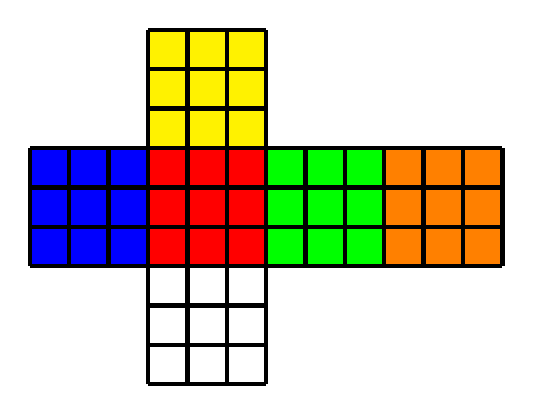
\begin{tikzpicture}[every node/.style={minimum size=0.5cm-\pgflinewidth, outer sep=0pt},scale=0.5]
    \node[fill=yellow] at (0.5,5.5) {};
    \node[fill=yellow] at (1.5,5.5) {};
    \node[fill=yellow] at (2.5,5.5) {};
    \node[fill=yellow] at (0.5,4.5) {};
    \node[fill=yellow] at (1.5,4.5) {};
    \node[fill=yellow] at (2.5,4.5) {};
    \node[fill=yellow] at (0.5,3.5) {};
    \node[fill=yellow] at (1.5,3.5) {};
    \node[fill=yellow] at (2.5,3.5) {};

    \node[fill=blue] at (-2.5,2.5) {};
    \node[fill=blue] at (-1.5,2.5) {};
    \node[fill=blue] at (-0.5,2.5) {};
    \node[fill=red] at (0.5,2.5) {};
    \node[fill=red] at (1.5,2.5) {};
    \node[fill=red] at (2.5,2.5) {};
    \node[fill=green] at (3.5,2.5) {};
    \node[fill=green] at (4.5,2.5) {};
    \node[fill=green] at (5.5,2.5) {};
    \node[fill=orange] at (6.5,2.5) {};
    \node[fill=orange] at (7.5,2.5) {};
    \node[fill=orange] at (8.5,2.5) {};

    \node[fill=blue] at (-2.5,1.5) {};
    \node[fill=blue] at (-1.5,1.5) {};
    \node[fill=blue] at (-0.5,1.5) {};
    \node[fill=red] at (0.5,1.5) {};
    \node[fill=red] at (1.5,1.5) {};
    \node[fill=red] at (2.5,1.5) {};
    \node[fill=green] at (3.5,1.5) {};
    \node[fill=green] at (4.5,1.5) {};
    \node[fill=green] at (5.5,1.5) {};
    \node[fill=orange] at (6.5,1.5) {};
    \node[fill=orange] at (7.5,1.5) {};
    \node[fill=orange] at (8.5,1.5) {};

    \node[fill=blue] at (-2.5,0.5) {};
    \node[fill=blue] at (-1.5,0.5) {};
    \node[fill=blue] at (-0.5,0.5) {};
    \node[fill=red] at (0.5,0.5) {};
    \node[fill=red] at (1.5,0.5) {};
    \node[fill=red] at (2.5,0.5) {};
    \node[fill=green] at (3.5,0.5) {};
    \node[fill=green] at (4.5,0.5) {};
    \node[fill=green] at (5.5,0.5) {};
    \node[fill=orange] at (6.5,0.5) {};
    \node[fill=orange] at (7.5,0.5) {};
    \node[fill=orange] at (8.5,0.5) {};

    \node[fill=white] at (0.5,-0.5) {};
    \node[fill=white] at (1.5,-0.5) {};
    \node[fill=white] at (2.5,-0.5) {};
    \node[fill=white] at (0.5,-1.5) {};
    \node[fill=white] at (1.5,-1.5) {};
    \node[fill=white] at (2.5,-1.5) {};
    \node[fill=white] at (0.5,-2.5) {};
    \node[fill=white] at (1.5,-2.5) {};
    \node[fill=white] at (2.5,-2.5) {};

    \draw[step=1cm,color=black, ultra thick] (-3,0) grid (9,3);
    \draw[step=1cm,color=black, ultra thick] (0,-3) grid (3,0);
    \draw[step=1cm,color=black, ultra thick] (0,3) grid (3,6);
\end{tikzpicture}

\vspace{0.5cm}
\textbf{\Large{Solutions}}

Each problem has only one solution. Solution can be accessed after each problem. You can apply the scramble in the solution to your Rubik's cube with yellow on the top and red on the front.

\vspace{0.5cm}
\textbf{\Large{Acknowledgement}}

Thanks to Xi'an Jiao Tong University Rubik's Cube Club, for providing the idea of ``Cube Sudoku".

\vspace{0.5cm}
\textbf{\Large{Github link}}

\href{https://github.com/nbwzx/CubeSudoku}{https://github.com/nbwzx/CubeSudoku}

\vspace{0.5cm}
\textbf{\Large{Contributors}}

\href{https://github.com/nbwzx}{Zixing Wang}


\vspace{0.5cm}
\textbf{\Large{License}}

MIT License
\pagebreak


{\noindent\Large  \newtime \textbf{No. 1\qquad Difficulty: $\bigstar$}}
\vspace{0.2cm}\\
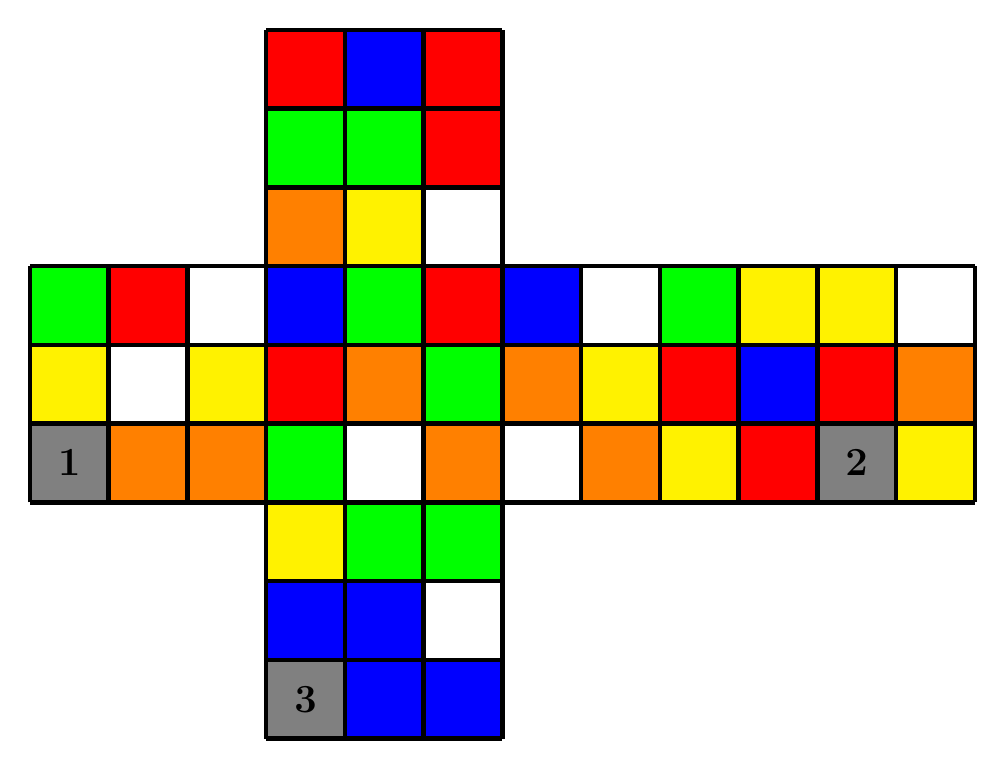
\begin{tikzpicture}[every node/.style={minimum size=1cm-\pgflinewidth, outer sep=0pt}]
\node[fill=red] at (0.5,5.5) {};
\node[fill=blue] at (1.5,5.5) {};
\node[fill=red] at (2.5,5.5) {};
\node[fill=green] at (0.5,4.5) {};
\node[fill=green] at (1.5,4.5) {};
\node[fill=red] at (2.5,4.5) {};
\node[fill=orange] at (0.5,3.5) {};
\node[fill=yellow] at (1.5,3.5) {};
\node[fill=white] at (2.5,3.5) {};

\node[fill=green] at (-2.5,2.5) {};
\node[fill=red] at (-1.5,2.5) {};
\node[fill=white] at (-0.5,2.5) {};
\node[fill=blue] at (0.5,2.5) {};
\node[fill=green] at (1.5,2.5) {};
\node[fill=red] at (2.5,2.5) {};
\node[fill=blue] at (3.5,2.5) {};
\node[fill=white] at (4.5,2.5) {};
\node[fill=green] at (5.5,2.5) {};
\node[fill=yellow] at (6.5,2.5) {};
\node[fill=yellow] at (7.5,2.5) {};
\node[fill=white] at (8.5,2.5) {};

\node[fill=yellow] at (-2.5,1.5) {};
\node[fill=white] at (-1.5,1.5) {};
\node[fill=yellow] at (-0.5,1.5) {};
\node[fill=red] at (0.5,1.5) {};
\node[fill=orange] at (1.5,1.5) {};
\node[fill=green] at (2.5,1.5) {};
\node[fill=orange] at (3.5,1.5) {};
\node[fill=yellow] at (4.5,1.5) {};
\node[fill=red] at (5.5,1.5) {};
\node[fill=blue] at (6.5,1.5) {};
\node[fill=red] at (7.5,1.5) {};
\node[fill=orange] at (8.5,1.5) {};

\node[fill=gray] at (-2.5,0.5) {\Large \textbf 1};
\node[fill=orange] at (-1.5,0.5) {};
\node[fill=orange] at (-0.5,0.5) {};
\node[fill=green] at (0.5,0.5) {};
\node[fill=white] at (1.5,0.5) {};
\node[fill=orange] at (2.5,0.5) {};
\node[fill=white] at (3.5,0.5) {};
\node[fill=orange] at (4.5,0.5) {};
\node[fill=yellow] at (5.5,0.5) {};
\node[fill=red] at (6.5,0.5) {};
\node[fill=gray] at (7.5,0.5) {\Large \textbf 2};
\node[fill=yellow] at (8.5,0.5) {};

\node[fill=yellow] at (0.5,-0.5) {};
\node[fill=green] at (1.5,-0.5) {};
\node[fill=green] at (2.5,-0.5) {};
\node[fill=blue] at (0.5,-1.5) {};
\node[fill=blue] at (1.5,-1.5) {};
\node[fill=white] at (2.5,-1.5) {};
\node[fill=gray] at (0.5,-2.5) {\Large \textbf 3};
\node[fill=blue] at (1.5,-2.5) {};
\node[fill=blue] at (2.5,-2.5) {};

\draw[step=1cm,color=black, ultra thick] (-3,0) grid (9,3);
\draw[step=1cm,color=black, ultra thick] (0,-3) grid (3,0);
\draw[step=1cm,color=black, ultra thick] (0,3) grid (3,6);
\end{tikzpicture}
\vspace{0.1cm}
\\
\noindent\normalsize \newtime  \textbf{Solution 1: F R L U' L U D' U R' D2 L F2 U B' U D' U F' D2 R' Fw' Uw2 }
\vspace{1cm}



{\noindent\Large  \newtime \textbf{No. 2\qquad Difficulty: $\bigstar$}}
\vspace{0.2cm}\\
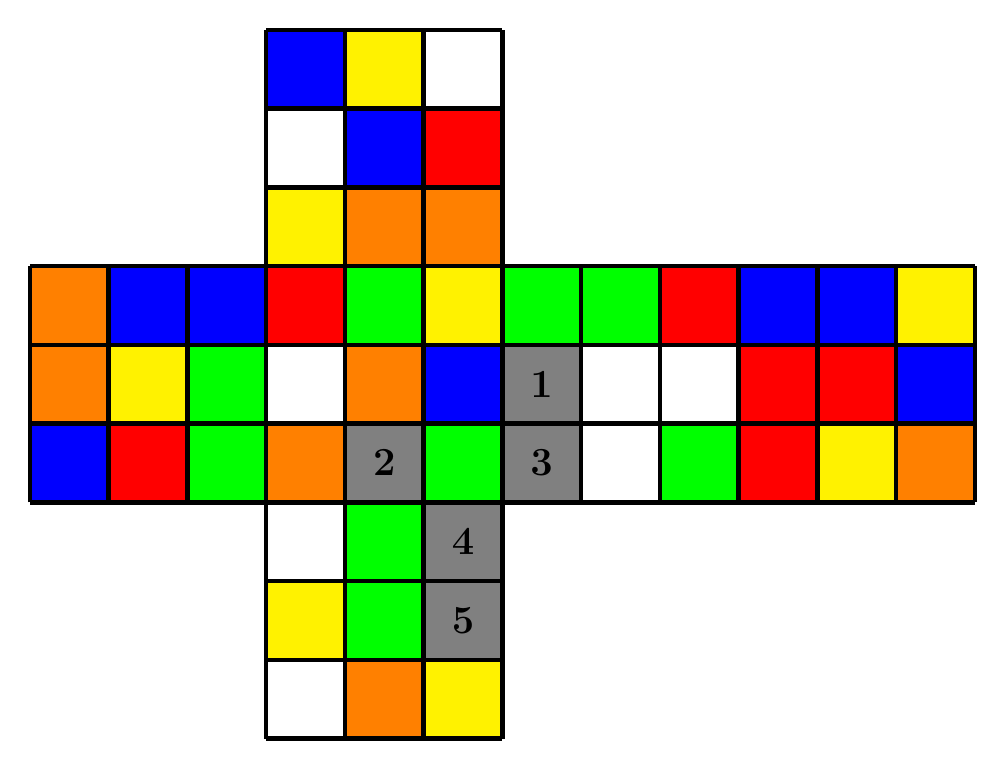
\begin{tikzpicture}[every node/.style={minimum size=1cm-\pgflinewidth, outer sep=0pt}]
\node[fill=blue] at (0.5,5.5) {};
\node[fill=yellow] at (1.5,5.5) {};
\node[fill=white] at (2.5,5.5) {};
\node[fill=white] at (0.5,4.5) {};
\node[fill=blue] at (1.5,4.5) {};
\node[fill=red] at (2.5,4.5) {};
\node[fill=yellow] at (0.5,3.5) {};
\node[fill=orange] at (1.5,3.5) {};
\node[fill=orange] at (2.5,3.5) {};

\node[fill=orange] at (-2.5,2.5) {};
\node[fill=blue] at (-1.5,2.5) {};
\node[fill=blue] at (-0.5,2.5) {};
\node[fill=red] at (0.5,2.5) {};
\node[fill=green] at (1.5,2.5) {};
\node[fill=yellow] at (2.5,2.5) {};
\node[fill=green] at (3.5,2.5) {};
\node[fill=green] at (4.5,2.5) {};
\node[fill=red] at (5.5,2.5) {};
\node[fill=blue] at (6.5,2.5) {};
\node[fill=blue] at (7.5,2.5) {};
\node[fill=yellow] at (8.5,2.5) {};

\node[fill=orange] at (-2.5,1.5) {};
\node[fill=yellow] at (-1.5,1.5) {};
\node[fill=green] at (-0.5,1.5) {};
\node[fill=white] at (0.5,1.5) {};
\node[fill=orange] at (1.5,1.5) {};
\node[fill=blue] at (2.5,1.5) {};
\node[fill=gray] at (3.5,1.5) {\Large \textbf 1};
\node[fill=white] at (4.5,1.5) {};
\node[fill=white] at (5.5,1.5) {};
\node[fill=red] at (6.5,1.5) {};
\node[fill=red] at (7.5,1.5) {};
\node[fill=blue] at (8.5,1.5) {};

\node[fill=blue] at (-2.5,0.5) {};
\node[fill=red] at (-1.5,0.5) {};
\node[fill=green] at (-0.5,0.5) {};
\node[fill=orange] at (0.5,0.5) {};
\node[fill=gray] at (1.5,0.5) {\Large \textbf 2};
\node[fill=green] at (2.5,0.5) {};
\node[fill=gray] at (3.5,0.5) {\Large \textbf 3};
\node[fill=white] at (4.5,0.5) {};
\node[fill=green] at (5.5,0.5) {};
\node[fill=red] at (6.5,0.5) {};
\node[fill=yellow] at (7.5,0.5) {};
\node[fill=orange] at (8.5,0.5) {};

\node[fill=white] at (0.5,-0.5) {};
\node[fill=green] at (1.5,-0.5) {};
\node[fill=gray] at (2.5,-0.5) {\Large \textbf 4};
\node[fill=yellow] at (0.5,-1.5) {};
\node[fill=green] at (1.5,-1.5) {};
\node[fill=gray] at (2.5,-1.5) {\Large \textbf 5};
\node[fill=white] at (0.5,-2.5) {};
\node[fill=orange] at (1.5,-2.5) {};
\node[fill=yellow] at (2.5,-2.5) {};

\draw[step=1cm,color=black, ultra thick] (-3,0) grid (9,3);
\draw[step=1cm,color=black, ultra thick] (0,-3) grid (3,0);
\draw[step=1cm,color=black, ultra thick] (0,3) grid (3,6);
\end{tikzpicture}
\vspace{0.1cm}
\\
\noindent\normalsize \newtime  \textbf{Solution 2: D2 B2 D2 R' L2 U D' B' L B L2 F2 D' F' U2 L2 F' U' D L' Fw Uw2 }
\vspace{1cm}



{\noindent\Large  \newtime \textbf{No. 3\qquad Difficulty: $\bigstar$}}
\vspace{0.2cm}\\
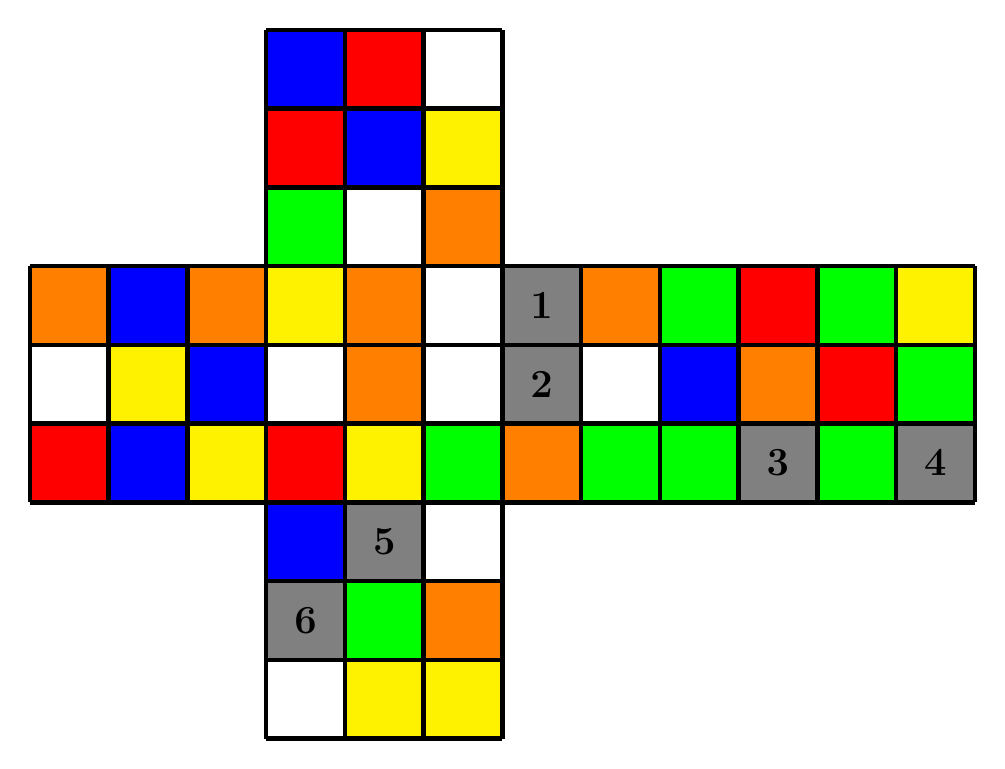
\begin{tikzpicture}[every node/.style={minimum size=1cm-\pgflinewidth, outer sep=0pt}]
\node[fill=blue] at (0.5,5.5) {};
\node[fill=red] at (1.5,5.5) {};
\node[fill=white] at (2.5,5.5) {};
\node[fill=red] at (0.5,4.5) {};
\node[fill=blue] at (1.5,4.5) {};
\node[fill=yellow] at (2.5,4.5) {};
\node[fill=green] at (0.5,3.5) {};
\node[fill=white] at (1.5,3.5) {};
\node[fill=orange] at (2.5,3.5) {};

\node[fill=orange] at (-2.5,2.5) {};
\node[fill=blue] at (-1.5,2.5) {};
\node[fill=orange] at (-0.5,2.5) {};
\node[fill=yellow] at (0.5,2.5) {};
\node[fill=orange] at (1.5,2.5) {};
\node[fill=white] at (2.5,2.5) {};
\node[fill=gray] at (3.5,2.5) {\Large \textbf 1};
\node[fill=orange] at (4.5,2.5) {};
\node[fill=green] at (5.5,2.5) {};
\node[fill=red] at (6.5,2.5) {};
\node[fill=green] at (7.5,2.5) {};
\node[fill=yellow] at (8.5,2.5) {};

\node[fill=white] at (-2.5,1.5) {};
\node[fill=yellow] at (-1.5,1.5) {};
\node[fill=blue] at (-0.5,1.5) {};
\node[fill=white] at (0.5,1.5) {};
\node[fill=orange] at (1.5,1.5) {};
\node[fill=white] at (2.5,1.5) {};
\node[fill=gray] at (3.5,1.5) {\Large \textbf 2};
\node[fill=white] at (4.5,1.5) {};
\node[fill=blue] at (5.5,1.5) {};
\node[fill=orange] at (6.5,1.5) {};
\node[fill=red] at (7.5,1.5) {};
\node[fill=green] at (8.5,1.5) {};

\node[fill=red] at (-2.5,0.5) {};
\node[fill=blue] at (-1.5,0.5) {};
\node[fill=yellow] at (-0.5,0.5) {};
\node[fill=red] at (0.5,0.5) {};
\node[fill=yellow] at (1.5,0.5) {};
\node[fill=green] at (2.5,0.5) {};
\node[fill=orange] at (3.5,0.5) {};
\node[fill=green] at (4.5,0.5) {};
\node[fill=green] at (5.5,0.5) {};
\node[fill=gray] at (6.5,0.5) {\Large \textbf 3};
\node[fill=green] at (7.5,0.5) {};
\node[fill=gray] at (8.5,0.5) {\Large \textbf 4};

\node[fill=blue] at (0.5,-0.5) {};
\node[fill=gray] at (1.5,-0.5) {\Large \textbf 5};
\node[fill=white] at (2.5,-0.5) {};
\node[fill=gray] at (0.5,-1.5) {\Large \textbf 6};
\node[fill=green] at (1.5,-1.5) {};
\node[fill=orange] at (2.5,-1.5) {};
\node[fill=white] at (0.5,-2.5) {};
\node[fill=yellow] at (1.5,-2.5) {};
\node[fill=yellow] at (2.5,-2.5) {};

\draw[step=1cm,color=black, ultra thick] (-3,0) grid (9,3);
\draw[step=1cm,color=black, ultra thick] (0,-3) grid (3,0);
\draw[step=1cm,color=black, ultra thick] (0,3) grid (3,6);
\end{tikzpicture}
\vspace{0.1cm}
\\
\noindent\normalsize \newtime  \textbf{Solution 3: U' D' B R F' L B F' U' B2 L' U L' D L2 U' B F' D2 U Fw Uw2 }
\vspace{1cm}



{\noindent\Large  \newtime \textbf{No. 4\qquad Difficulty: $\bigstar$}}
\vspace{0.2cm}\\
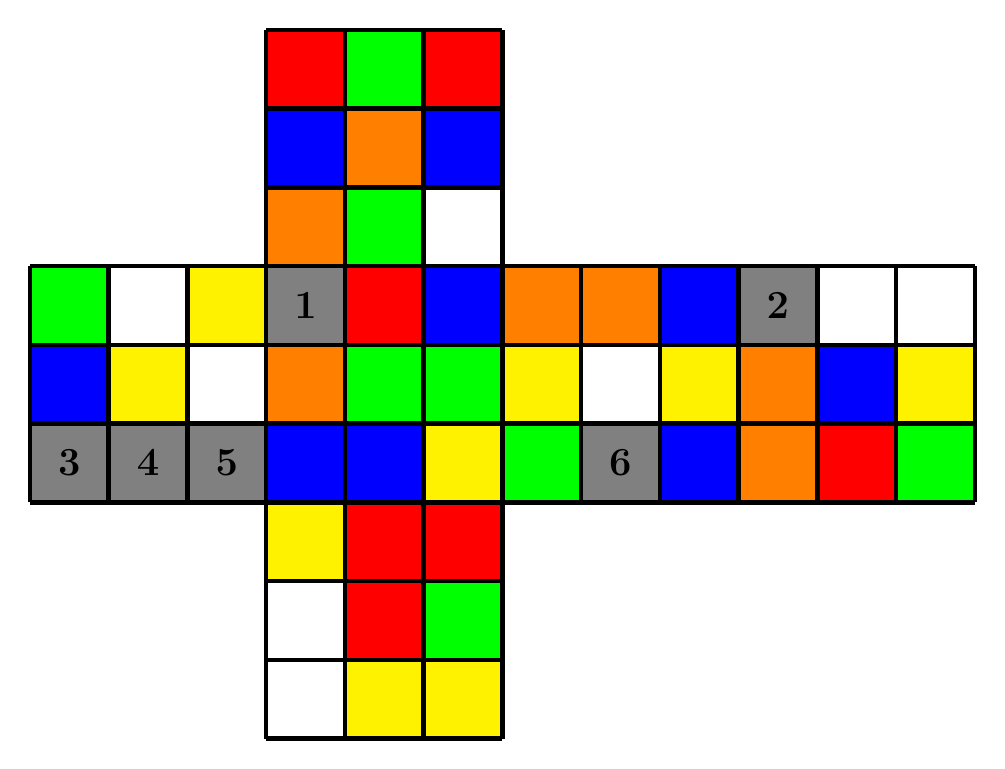
\begin{tikzpicture}[every node/.style={minimum size=1cm-\pgflinewidth, outer sep=0pt}]
\node[fill=red] at (0.5,5.5) {};
\node[fill=green] at (1.5,5.5) {};
\node[fill=red] at (2.5,5.5) {};
\node[fill=blue] at (0.5,4.5) {};
\node[fill=orange] at (1.5,4.5) {};
\node[fill=blue] at (2.5,4.5) {};
\node[fill=orange] at (0.5,3.5) {};
\node[fill=green] at (1.5,3.5) {};
\node[fill=white] at (2.5,3.5) {};

\node[fill=green] at (-2.5,2.5) {};
\node[fill=white] at (-1.5,2.5) {};
\node[fill=yellow] at (-0.5,2.5) {};
\node[fill=gray] at (0.5,2.5) {\Large \textbf 1};
\node[fill=red] at (1.5,2.5) {};
\node[fill=blue] at (2.5,2.5) {};
\node[fill=orange] at (3.5,2.5) {};
\node[fill=orange] at (4.5,2.5) {};
\node[fill=blue] at (5.5,2.5) {};
\node[fill=gray] at (6.5,2.5) {\Large \textbf 2};
\node[fill=white] at (7.5,2.5) {};
\node[fill=white] at (8.5,2.5) {};

\node[fill=blue] at (-2.5,1.5) {};
\node[fill=yellow] at (-1.5,1.5) {};
\node[fill=white] at (-0.5,1.5) {};
\node[fill=orange] at (0.5,1.5) {};
\node[fill=green] at (1.5,1.5) {};
\node[fill=green] at (2.5,1.5) {};
\node[fill=yellow] at (3.5,1.5) {};
\node[fill=white] at (4.5,1.5) {};
\node[fill=yellow] at (5.5,1.5) {};
\node[fill=orange] at (6.5,1.5) {};
\node[fill=blue] at (7.5,1.5) {};
\node[fill=yellow] at (8.5,1.5) {};

\node[fill=gray] at (-2.5,0.5) {\Large \textbf 3};
\node[fill=gray] at (-1.5,0.5) {\Large \textbf 4};
\node[fill=gray] at (-0.5,0.5) {\Large \textbf 5};
\node[fill=blue] at (0.5,0.5) {};
\node[fill=blue] at (1.5,0.5) {};
\node[fill=yellow] at (2.5,0.5) {};
\node[fill=green] at (3.5,0.5) {};
\node[fill=gray] at (4.5,0.5) {\Large \textbf 6};
\node[fill=blue] at (5.5,0.5) {};
\node[fill=orange] at (6.5,0.5) {};
\node[fill=red] at (7.5,0.5) {};
\node[fill=green] at (8.5,0.5) {};

\node[fill=yellow] at (0.5,-0.5) {};
\node[fill=red] at (1.5,-0.5) {};
\node[fill=red] at (2.5,-0.5) {};
\node[fill=white] at (0.5,-1.5) {};
\node[fill=red] at (1.5,-1.5) {};
\node[fill=green] at (2.5,-1.5) {};
\node[fill=white] at (0.5,-2.5) {};
\node[fill=yellow] at (1.5,-2.5) {};
\node[fill=yellow] at (2.5,-2.5) {};

\draw[step=1cm,color=black, ultra thick] (-3,0) grid (9,3);
\draw[step=1cm,color=black, ultra thick] (0,-3) grid (3,0);
\draw[step=1cm,color=black, ultra thick] (0,3) grid (3,6);
\end{tikzpicture}
\vspace{0.1cm}
\\
\noindent\normalsize \newtime  \textbf{Solution 4: B' D2 U' F' B2 R' B' U F' B' U2 D' L' B2 U2 F' D' L' B2 D' Rw' Uw }
\vspace{1cm}



{\noindent\Large  \newtime \textbf{No. 5\qquad Difficulty: $\bigstar$}}
\vspace{0.2cm}\\
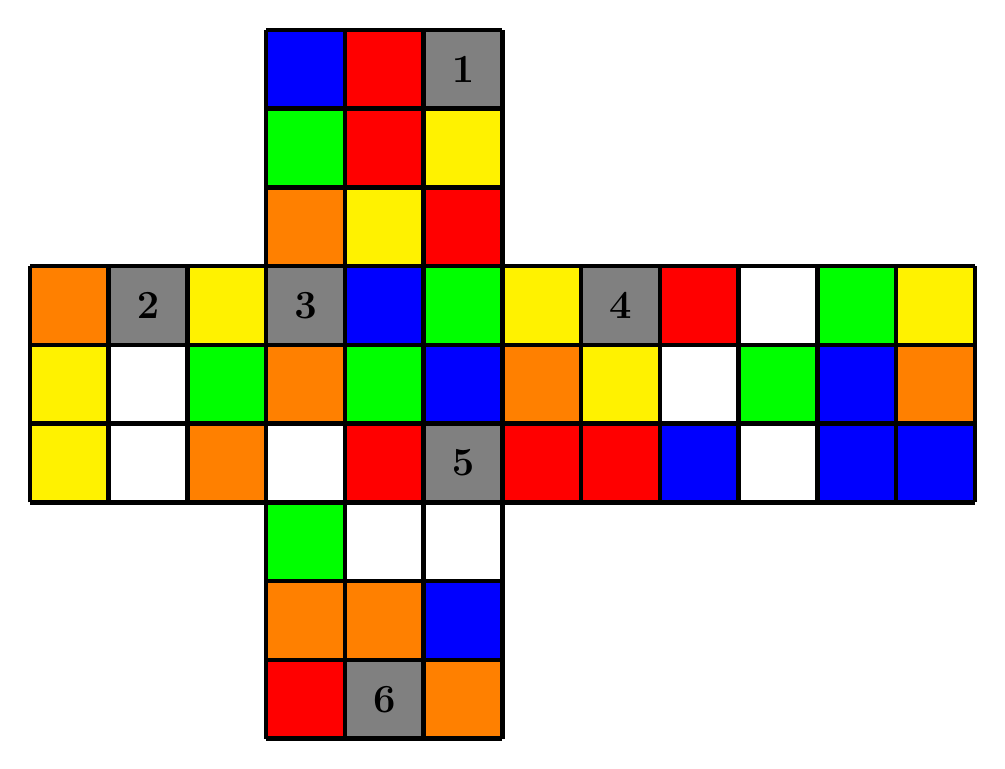
\begin{tikzpicture}[every node/.style={minimum size=1cm-\pgflinewidth, outer sep=0pt}]
\node[fill=blue] at (0.5,5.5) {};
\node[fill=red] at (1.5,5.5) {};
\node[fill=gray] at (2.5,5.5) {\Large \textbf 1};
\node[fill=green] at (0.5,4.5) {};
\node[fill=red] at (1.5,4.5) {};
\node[fill=yellow] at (2.5,4.5) {};
\node[fill=orange] at (0.5,3.5) {};
\node[fill=yellow] at (1.5,3.5) {};
\node[fill=red] at (2.5,3.5) {};

\node[fill=orange] at (-2.5,2.5) {};
\node[fill=gray] at (-1.5,2.5) {\Large \textbf 2};
\node[fill=yellow] at (-0.5,2.5) {};
\node[fill=gray] at (0.5,2.5) {\Large \textbf 3};
\node[fill=blue] at (1.5,2.5) {};
\node[fill=green] at (2.5,2.5) {};
\node[fill=yellow] at (3.5,2.5) {};
\node[fill=gray] at (4.5,2.5) {\Large \textbf 4};
\node[fill=red] at (5.5,2.5) {};
\node[fill=white] at (6.5,2.5) {};
\node[fill=green] at (7.5,2.5) {};
\node[fill=yellow] at (8.5,2.5) {};

\node[fill=yellow] at (-2.5,1.5) {};
\node[fill=white] at (-1.5,1.5) {};
\node[fill=green] at (-0.5,1.5) {};
\node[fill=orange] at (0.5,1.5) {};
\node[fill=green] at (1.5,1.5) {};
\node[fill=blue] at (2.5,1.5) {};
\node[fill=orange] at (3.5,1.5) {};
\node[fill=yellow] at (4.5,1.5) {};
\node[fill=white] at (5.5,1.5) {};
\node[fill=green] at (6.5,1.5) {};
\node[fill=blue] at (7.5,1.5) {};
\node[fill=orange] at (8.5,1.5) {};

\node[fill=yellow] at (-2.5,0.5) {};
\node[fill=white] at (-1.5,0.5) {};
\node[fill=orange] at (-0.5,0.5) {};
\node[fill=white] at (0.5,0.5) {};
\node[fill=red] at (1.5,0.5) {};
\node[fill=gray] at (2.5,0.5) {\Large \textbf 5};
\node[fill=red] at (3.5,0.5) {};
\node[fill=red] at (4.5,0.5) {};
\node[fill=blue] at (5.5,0.5) {};
\node[fill=white] at (6.5,0.5) {};
\node[fill=blue] at (7.5,0.5) {};
\node[fill=blue] at (8.5,0.5) {};

\node[fill=green] at (0.5,-0.5) {};
\node[fill=white] at (1.5,-0.5) {};
\node[fill=white] at (2.5,-0.5) {};
\node[fill=orange] at (0.5,-1.5) {};
\node[fill=orange] at (1.5,-1.5) {};
\node[fill=blue] at (2.5,-1.5) {};
\node[fill=red] at (0.5,-2.5) {};
\node[fill=gray] at (1.5,-2.5) {\Large \textbf 6};
\node[fill=orange] at (2.5,-2.5) {};

\draw[step=1cm,color=black, ultra thick] (-3,0) grid (9,3);
\draw[step=1cm,color=black, ultra thick] (0,-3) grid (3,0);
\draw[step=1cm,color=black, ultra thick] (0,3) grid (3,6);
\end{tikzpicture}
\vspace{0.1cm}
\\
\noindent\normalsize \newtime  \textbf{Solution 5: B' F2 R' U D2 B R B' R2 D R U R' U R2 D2 R2 L B L2 Rw Uw }
\vspace{1cm}



{\noindent\Large  \newtime \textbf{No. 6\qquad Difficulty: $\bigstar$}}
\vspace{0.2cm}\\
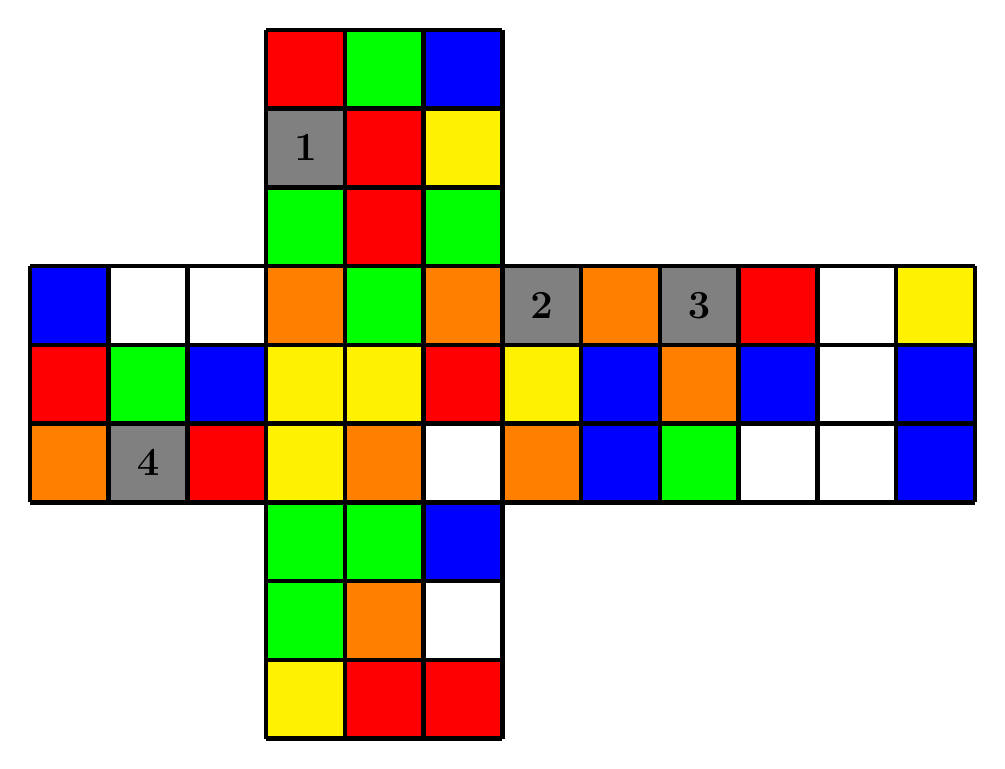
\begin{tikzpicture}[every node/.style={minimum size=1cm-\pgflinewidth, outer sep=0pt}]
\node[fill=red] at (0.5,5.5) {};
\node[fill=green] at (1.5,5.5) {};
\node[fill=blue] at (2.5,5.5) {};
\node[fill=gray] at (0.5,4.5) {\Large \textbf 1};
\node[fill=red] at (1.5,4.5) {};
\node[fill=yellow] at (2.5,4.5) {};
\node[fill=green] at (0.5,3.5) {};
\node[fill=red] at (1.5,3.5) {};
\node[fill=green] at (2.5,3.5) {};

\node[fill=blue] at (-2.5,2.5) {};
\node[fill=white] at (-1.5,2.5) {};
\node[fill=white] at (-0.5,2.5) {};
\node[fill=orange] at (0.5,2.5) {};
\node[fill=green] at (1.5,2.5) {};
\node[fill=orange] at (2.5,2.5) {};
\node[fill=gray] at (3.5,2.5) {\Large \textbf 2};
\node[fill=orange] at (4.5,2.5) {};
\node[fill=gray] at (5.5,2.5) {\Large \textbf 3};
\node[fill=red] at (6.5,2.5) {};
\node[fill=white] at (7.5,2.5) {};
\node[fill=yellow] at (8.5,2.5) {};

\node[fill=red] at (-2.5,1.5) {};
\node[fill=green] at (-1.5,1.5) {};
\node[fill=blue] at (-0.5,1.5) {};
\node[fill=yellow] at (0.5,1.5) {};
\node[fill=yellow] at (1.5,1.5) {};
\node[fill=red] at (2.5,1.5) {};
\node[fill=yellow] at (3.5,1.5) {};
\node[fill=blue] at (4.5,1.5) {};
\node[fill=orange] at (5.5,1.5) {};
\node[fill=blue] at (6.5,1.5) {};
\node[fill=white] at (7.5,1.5) {};
\node[fill=blue] at (8.5,1.5) {};

\node[fill=orange] at (-2.5,0.5) {};
\node[fill=gray] at (-1.5,0.5) {\Large \textbf 4};
\node[fill=red] at (-0.5,0.5) {};
\node[fill=yellow] at (0.5,0.5) {};
\node[fill=orange] at (1.5,0.5) {};
\node[fill=white] at (2.5,0.5) {};
\node[fill=orange] at (3.5,0.5) {};
\node[fill=blue] at (4.5,0.5) {};
\node[fill=green] at (5.5,0.5) {};
\node[fill=white] at (6.5,0.5) {};
\node[fill=white] at (7.5,0.5) {};
\node[fill=blue] at (8.5,0.5) {};

\node[fill=green] at (0.5,-0.5) {};
\node[fill=green] at (1.5,-0.5) {};
\node[fill=blue] at (2.5,-0.5) {};
\node[fill=green] at (0.5,-1.5) {};
\node[fill=orange] at (1.5,-1.5) {};
\node[fill=white] at (2.5,-1.5) {};
\node[fill=yellow] at (0.5,-2.5) {};
\node[fill=red] at (1.5,-2.5) {};
\node[fill=red] at (2.5,-2.5) {};

\draw[step=1cm,color=black, ultra thick] (-3,0) grid (9,3);
\draw[step=1cm,color=black, ultra thick] (0,-3) grid (3,0);
\draw[step=1cm,color=black, ultra thick] (0,3) grid (3,6);
\end{tikzpicture}
\vspace{0.1cm}
\\
\noindent\normalsize \newtime  \textbf{Solution 6: B R2 F' B R2 L2 F2 L' U L2 U' F2 D' U2 R2 L F' U2 D' F Rw Uw2 }
\vspace{1cm}



{\noindent\Large  \newtime \textbf{No. 7\qquad Difficulty: $\bigstar$}}
\vspace{0.2cm}\\
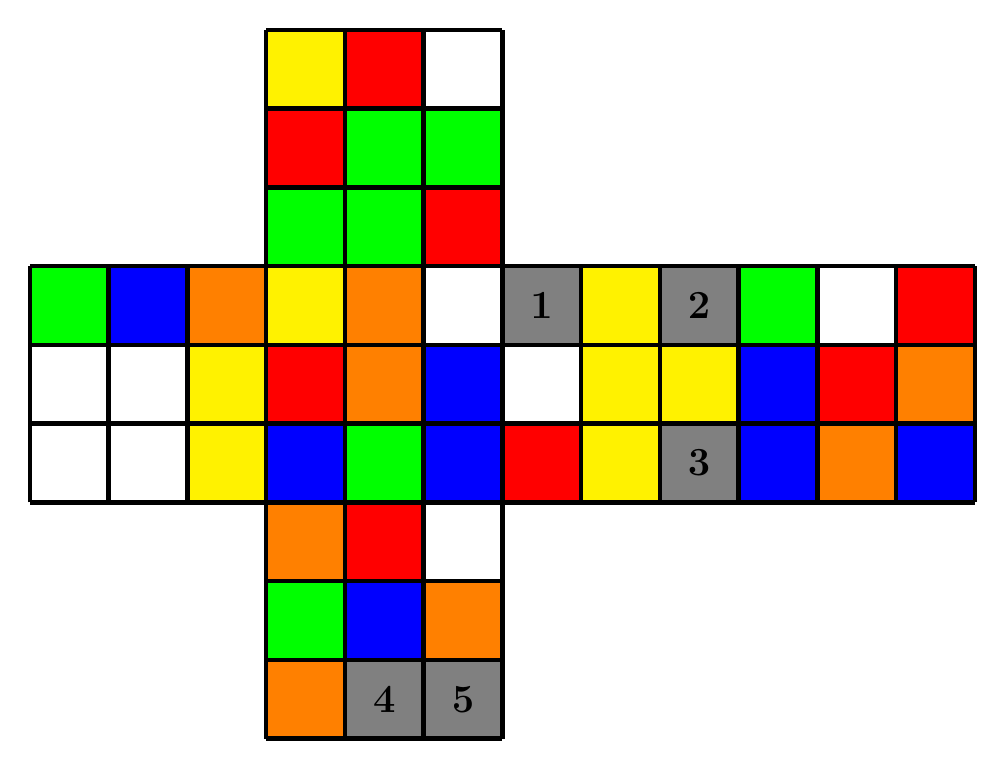
\begin{tikzpicture}[every node/.style={minimum size=1cm-\pgflinewidth, outer sep=0pt}]
\node[fill=yellow] at (0.5,5.5) {};
\node[fill=red] at (1.5,5.5) {};
\node[fill=white] at (2.5,5.5) {};
\node[fill=red] at (0.5,4.5) {};
\node[fill=green] at (1.5,4.5) {};
\node[fill=green] at (2.5,4.5) {};
\node[fill=green] at (0.5,3.5) {};
\node[fill=green] at (1.5,3.5) {};
\node[fill=red] at (2.5,3.5) {};

\node[fill=green] at (-2.5,2.5) {};
\node[fill=blue] at (-1.5,2.5) {};
\node[fill=orange] at (-0.5,2.5) {};
\node[fill=yellow] at (0.5,2.5) {};
\node[fill=orange] at (1.5,2.5) {};
\node[fill=white] at (2.5,2.5) {};
\node[fill=gray] at (3.5,2.5) {\Large \textbf 1};
\node[fill=yellow] at (4.5,2.5) {};
\node[fill=gray] at (5.5,2.5) {\Large \textbf 2};
\node[fill=green] at (6.5,2.5) {};
\node[fill=white] at (7.5,2.5) {};
\node[fill=red] at (8.5,2.5) {};

\node[fill=white] at (-2.5,1.5) {};
\node[fill=white] at (-1.5,1.5) {};
\node[fill=yellow] at (-0.5,1.5) {};
\node[fill=red] at (0.5,1.5) {};
\node[fill=orange] at (1.5,1.5) {};
\node[fill=blue] at (2.5,1.5) {};
\node[fill=white] at (3.5,1.5) {};
\node[fill=yellow] at (4.5,1.5) {};
\node[fill=yellow] at (5.5,1.5) {};
\node[fill=blue] at (6.5,1.5) {};
\node[fill=red] at (7.5,1.5) {};
\node[fill=orange] at (8.5,1.5) {};

\node[fill=white] at (-2.5,0.5) {};
\node[fill=white] at (-1.5,0.5) {};
\node[fill=yellow] at (-0.5,0.5) {};
\node[fill=blue] at (0.5,0.5) {};
\node[fill=green] at (1.5,0.5) {};
\node[fill=blue] at (2.5,0.5) {};
\node[fill=red] at (3.5,0.5) {};
\node[fill=yellow] at (4.5,0.5) {};
\node[fill=gray] at (5.5,0.5) {\Large \textbf 3};
\node[fill=blue] at (6.5,0.5) {};
\node[fill=orange] at (7.5,0.5) {};
\node[fill=blue] at (8.5,0.5) {};

\node[fill=orange] at (0.5,-0.5) {};
\node[fill=red] at (1.5,-0.5) {};
\node[fill=white] at (2.5,-0.5) {};
\node[fill=green] at (0.5,-1.5) {};
\node[fill=blue] at (1.5,-1.5) {};
\node[fill=orange] at (2.5,-1.5) {};
\node[fill=orange] at (0.5,-2.5) {};
\node[fill=gray] at (1.5,-2.5) {\Large \textbf 4};
\node[fill=gray] at (2.5,-2.5) {\Large \textbf 5};

\draw[step=1cm,color=black, ultra thick] (-3,0) grid (9,3);
\draw[step=1cm,color=black, ultra thick] (0,-3) grid (3,0);
\draw[step=1cm,color=black, ultra thick] (0,3) grid (3,6);
\end{tikzpicture}
\vspace{0.1cm}
\\
\noindent\normalsize \newtime  \textbf{Solution 7: B R' F' D' B' D2 F' R' D2 F' U F2 D' L2 F U2 D L2 R B Fw' Uw2 }
\vspace{1cm}



{\noindent\Large  \newtime \textbf{No. 8\qquad Difficulty: $\bigstar$}}
\vspace{0.2cm}\\
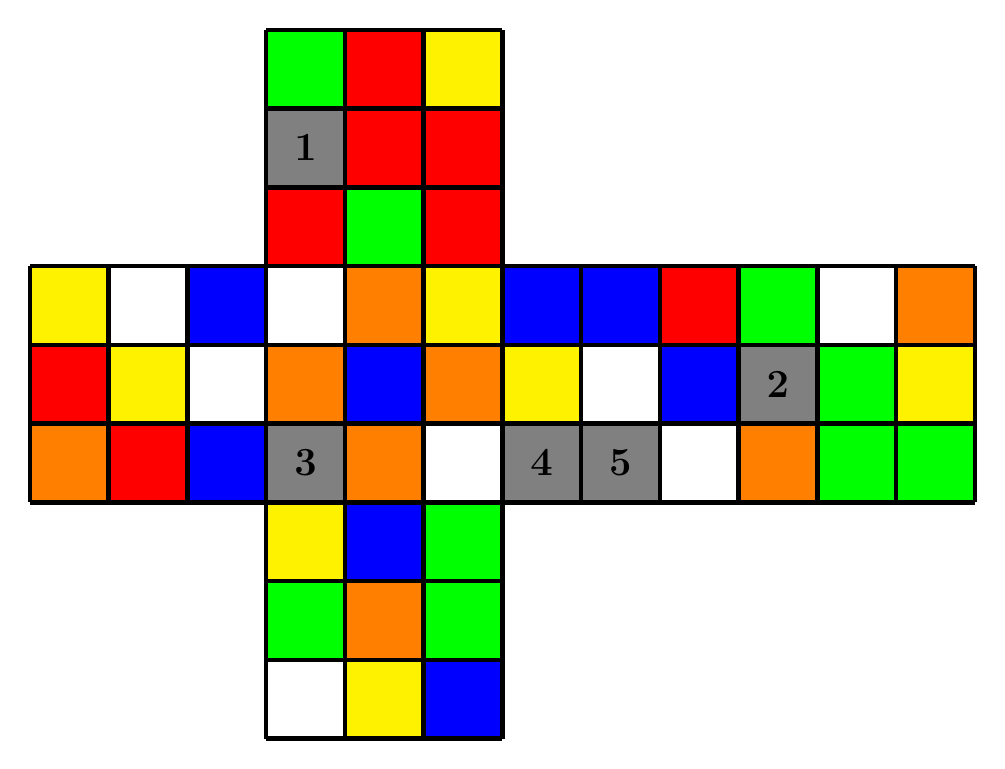
\begin{tikzpicture}[every node/.style={minimum size=1cm-\pgflinewidth, outer sep=0pt}]
\node[fill=green] at (0.5,5.5) {};
\node[fill=red] at (1.5,5.5) {};
\node[fill=yellow] at (2.5,5.5) {};
\node[fill=gray] at (0.5,4.5) {\Large \textbf 1};
\node[fill=red] at (1.5,4.5) {};
\node[fill=red] at (2.5,4.5) {};
\node[fill=red] at (0.5,3.5) {};
\node[fill=green] at (1.5,3.5) {};
\node[fill=red] at (2.5,3.5) {};

\node[fill=yellow] at (-2.5,2.5) {};
\node[fill=white] at (-1.5,2.5) {};
\node[fill=blue] at (-0.5,2.5) {};
\node[fill=white] at (0.5,2.5) {};
\node[fill=orange] at (1.5,2.5) {};
\node[fill=yellow] at (2.5,2.5) {};
\node[fill=blue] at (3.5,2.5) {};
\node[fill=blue] at (4.5,2.5) {};
\node[fill=red] at (5.5,2.5) {};
\node[fill=green] at (6.5,2.5) {};
\node[fill=white] at (7.5,2.5) {};
\node[fill=orange] at (8.5,2.5) {};

\node[fill=red] at (-2.5,1.5) {};
\node[fill=yellow] at (-1.5,1.5) {};
\node[fill=white] at (-0.5,1.5) {};
\node[fill=orange] at (0.5,1.5) {};
\node[fill=blue] at (1.5,1.5) {};
\node[fill=orange] at (2.5,1.5) {};
\node[fill=yellow] at (3.5,1.5) {};
\node[fill=white] at (4.5,1.5) {};
\node[fill=blue] at (5.5,1.5) {};
\node[fill=gray] at (6.5,1.5) {\Large \textbf 2};
\node[fill=green] at (7.5,1.5) {};
\node[fill=yellow] at (8.5,1.5) {};

\node[fill=orange] at (-2.5,0.5) {};
\node[fill=red] at (-1.5,0.5) {};
\node[fill=blue] at (-0.5,0.5) {};
\node[fill=gray] at (0.5,0.5) {\Large \textbf 3};
\node[fill=orange] at (1.5,0.5) {};
\node[fill=white] at (2.5,0.5) {};
\node[fill=gray] at (3.5,0.5) {\Large \textbf 4};
\node[fill=gray] at (4.5,0.5) {\Large \textbf 5};
\node[fill=white] at (5.5,0.5) {};
\node[fill=orange] at (6.5,0.5) {};
\node[fill=green] at (7.5,0.5) {};
\node[fill=green] at (8.5,0.5) {};

\node[fill=yellow] at (0.5,-0.5) {};
\node[fill=blue] at (1.5,-0.5) {};
\node[fill=green] at (2.5,-0.5) {};
\node[fill=green] at (0.5,-1.5) {};
\node[fill=orange] at (1.5,-1.5) {};
\node[fill=green] at (2.5,-1.5) {};
\node[fill=white] at (0.5,-2.5) {};
\node[fill=yellow] at (1.5,-2.5) {};
\node[fill=blue] at (2.5,-2.5) {};

\draw[step=1cm,color=black, ultra thick] (-3,0) grid (9,3);
\draw[step=1cm,color=black, ultra thick] (0,-3) grid (3,0);
\draw[step=1cm,color=black, ultra thick] (0,3) grid (3,6);
\end{tikzpicture}
\vspace{0.1cm}
\\
\noindent\normalsize \newtime  \textbf{Solution 8: R2 F U B' D U2 R' B F' D U' B2 L U2 D' L' U' L2 F' L' Rw Uw' }
\vspace{1cm}



{\noindent\Large  \newtime \textbf{No. 9\qquad Difficulty: $\bigstar$}}
\vspace{0.2cm}\\
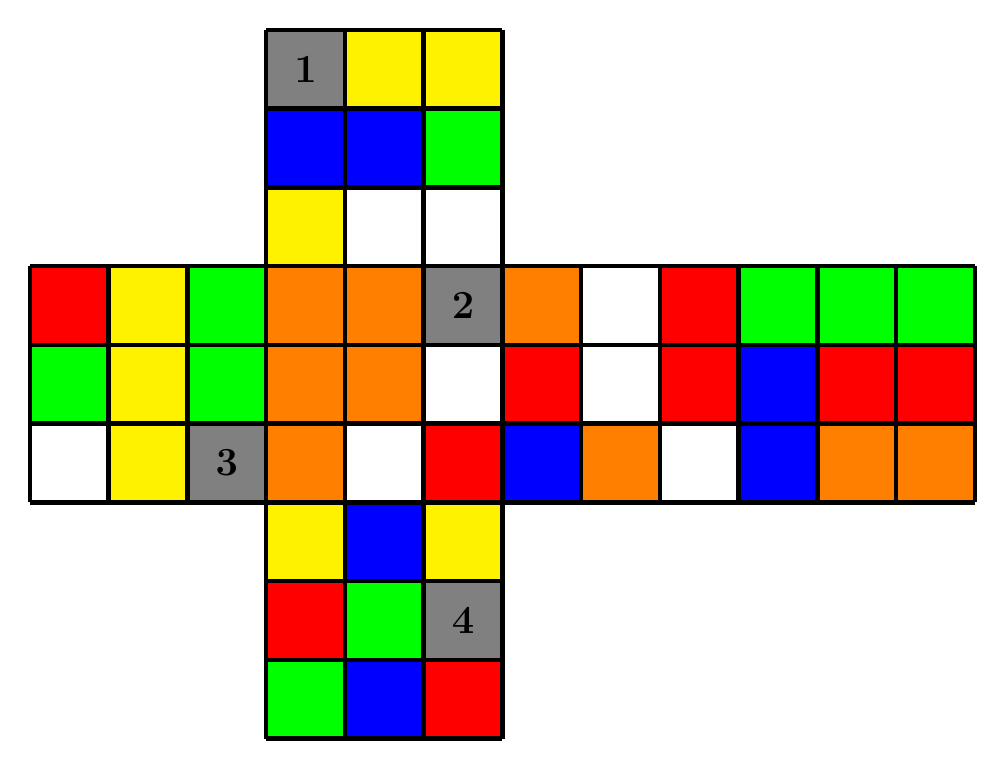
\begin{tikzpicture}[every node/.style={minimum size=1cm-\pgflinewidth, outer sep=0pt}]
\node[fill=gray] at (0.5,5.5) {\Large \textbf 1};
\node[fill=yellow] at (1.5,5.5) {};
\node[fill=yellow] at (2.5,5.5) {};
\node[fill=blue] at (0.5,4.5) {};
\node[fill=blue] at (1.5,4.5) {};
\node[fill=green] at (2.5,4.5) {};
\node[fill=yellow] at (0.5,3.5) {};
\node[fill=white] at (1.5,3.5) {};
\node[fill=white] at (2.5,3.5) {};

\node[fill=red] at (-2.5,2.5) {};
\node[fill=yellow] at (-1.5,2.5) {};
\node[fill=green] at (-0.5,2.5) {};
\node[fill=orange] at (0.5,2.5) {};
\node[fill=orange] at (1.5,2.5) {};
\node[fill=gray] at (2.5,2.5) {\Large \textbf 2};
\node[fill=orange] at (3.5,2.5) {};
\node[fill=white] at (4.5,2.5) {};
\node[fill=red] at (5.5,2.5) {};
\node[fill=green] at (6.5,2.5) {};
\node[fill=green] at (7.5,2.5) {};
\node[fill=green] at (8.5,2.5) {};

\node[fill=green] at (-2.5,1.5) {};
\node[fill=yellow] at (-1.5,1.5) {};
\node[fill=green] at (-0.5,1.5) {};
\node[fill=orange] at (0.5,1.5) {};
\node[fill=orange] at (1.5,1.5) {};
\node[fill=white] at (2.5,1.5) {};
\node[fill=red] at (3.5,1.5) {};
\node[fill=white] at (4.5,1.5) {};
\node[fill=red] at (5.5,1.5) {};
\node[fill=blue] at (6.5,1.5) {};
\node[fill=red] at (7.5,1.5) {};
\node[fill=red] at (8.5,1.5) {};

\node[fill=white] at (-2.5,0.5) {};
\node[fill=yellow] at (-1.5,0.5) {};
\node[fill=gray] at (-0.5,0.5) {\Large \textbf 3};
\node[fill=orange] at (0.5,0.5) {};
\node[fill=white] at (1.5,0.5) {};
\node[fill=red] at (2.5,0.5) {};
\node[fill=blue] at (3.5,0.5) {};
\node[fill=orange] at (4.5,0.5) {};
\node[fill=white] at (5.5,0.5) {};
\node[fill=blue] at (6.5,0.5) {};
\node[fill=orange] at (7.5,0.5) {};
\node[fill=orange] at (8.5,0.5) {};

\node[fill=yellow] at (0.5,-0.5) {};
\node[fill=blue] at (1.5,-0.5) {};
\node[fill=yellow] at (2.5,-0.5) {};
\node[fill=red] at (0.5,-1.5) {};
\node[fill=green] at (1.5,-1.5) {};
\node[fill=gray] at (2.5,-1.5) {\Large \textbf 4};
\node[fill=green] at (0.5,-2.5) {};
\node[fill=blue] at (1.5,-2.5) {};
\node[fill=red] at (2.5,-2.5) {};

\draw[step=1cm,color=black, ultra thick] (-3,0) grid (9,3);
\draw[step=1cm,color=black, ultra thick] (0,-3) grid (3,0);
\draw[step=1cm,color=black, ultra thick] (0,3) grid (3,6);
\end{tikzpicture}
\vspace{0.1cm}
\\
\noindent\normalsize \newtime  \textbf{Solution 9: U' L2 U B U2 F2 D' U2 R2 L U' B' L' B' D2 R D R F B Fw Uw2 }
\vspace{1cm}



{\noindent\Large  \newtime \textbf{No. 10\qquad Difficulty: $\bigstar$}}
\vspace{0.2cm}\\
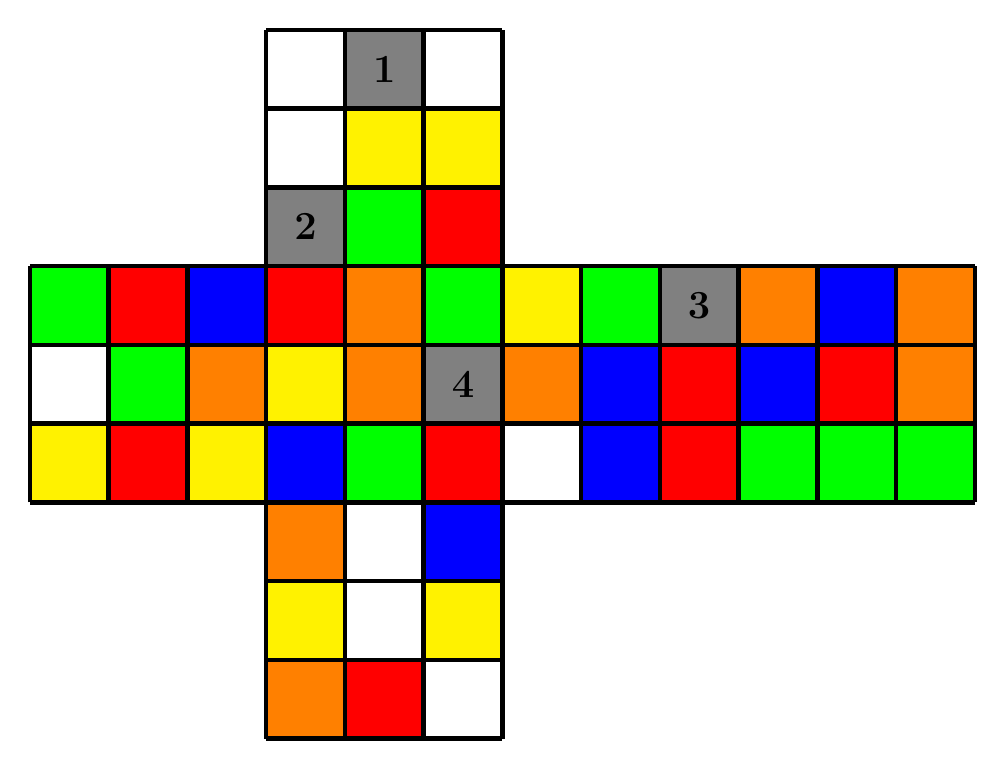
\begin{tikzpicture}[every node/.style={minimum size=1cm-\pgflinewidth, outer sep=0pt}]
\node[fill=white] at (0.5,5.5) {};
\node[fill=gray] at (1.5,5.5) {\Large \textbf 1};
\node[fill=white] at (2.5,5.5) {};
\node[fill=white] at (0.5,4.5) {};
\node[fill=yellow] at (1.5,4.5) {};
\node[fill=yellow] at (2.5,4.5) {};
\node[fill=gray] at (0.5,3.5) {\Large \textbf 2};
\node[fill=green] at (1.5,3.5) {};
\node[fill=red] at (2.5,3.5) {};

\node[fill=green] at (-2.5,2.5) {};
\node[fill=red] at (-1.5,2.5) {};
\node[fill=blue] at (-0.5,2.5) {};
\node[fill=red] at (0.5,2.5) {};
\node[fill=orange] at (1.5,2.5) {};
\node[fill=green] at (2.5,2.5) {};
\node[fill=yellow] at (3.5,2.5) {};
\node[fill=green] at (4.5,2.5) {};
\node[fill=gray] at (5.5,2.5) {\Large \textbf 3};
\node[fill=orange] at (6.5,2.5) {};
\node[fill=blue] at (7.5,2.5) {};
\node[fill=orange] at (8.5,2.5) {};

\node[fill=white] at (-2.5,1.5) {};
\node[fill=green] at (-1.5,1.5) {};
\node[fill=orange] at (-0.5,1.5) {};
\node[fill=yellow] at (0.5,1.5) {};
\node[fill=orange] at (1.5,1.5) {};
\node[fill=gray] at (2.5,1.5) {\Large \textbf 4};
\node[fill=orange] at (3.5,1.5) {};
\node[fill=blue] at (4.5,1.5) {};
\node[fill=red] at (5.5,1.5) {};
\node[fill=blue] at (6.5,1.5) {};
\node[fill=red] at (7.5,1.5) {};
\node[fill=orange] at (8.5,1.5) {};

\node[fill=yellow] at (-2.5,0.5) {};
\node[fill=red] at (-1.5,0.5) {};
\node[fill=yellow] at (-0.5,0.5) {};
\node[fill=blue] at (0.5,0.5) {};
\node[fill=green] at (1.5,0.5) {};
\node[fill=red] at (2.5,0.5) {};
\node[fill=white] at (3.5,0.5) {};
\node[fill=blue] at (4.5,0.5) {};
\node[fill=red] at (5.5,0.5) {};
\node[fill=green] at (6.5,0.5) {};
\node[fill=green] at (7.5,0.5) {};
\node[fill=green] at (8.5,0.5) {};

\node[fill=orange] at (0.5,-0.5) {};
\node[fill=white] at (1.5,-0.5) {};
\node[fill=blue] at (2.5,-0.5) {};
\node[fill=yellow] at (0.5,-1.5) {};
\node[fill=white] at (1.5,-1.5) {};
\node[fill=yellow] at (2.5,-1.5) {};
\node[fill=orange] at (0.5,-2.5) {};
\node[fill=red] at (1.5,-2.5) {};
\node[fill=white] at (2.5,-2.5) {};

\draw[step=1cm,color=black, ultra thick] (-3,0) grid (9,3);
\draw[step=1cm,color=black, ultra thick] (0,-3) grid (3,0);
\draw[step=1cm,color=black, ultra thick] (0,3) grid (3,6);
\end{tikzpicture}
\vspace{0.1cm}
\\
\noindent\normalsize \newtime  \textbf{Solution 10: U2 R2 F2 R2 B2 F2 L D2 L' F B' L F2 D R U' F L U' R Uw2 }
\vspace{1cm}



{\noindent\Large  \newtime \textbf{No. 11\qquad Difficulty: $\bigstar$}}
\vspace{0.2cm}\\
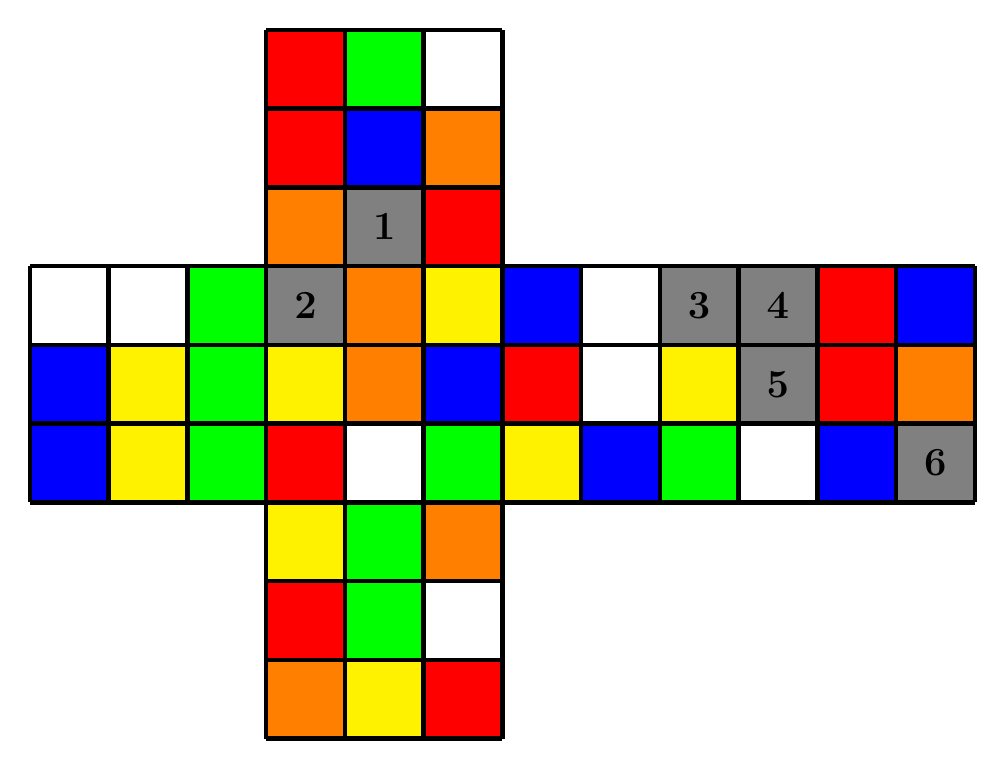
\begin{tikzpicture}[every node/.style={minimum size=1cm-\pgflinewidth, outer sep=0pt}]
\node[fill=red] at (0.5,5.5) {};
\node[fill=green] at (1.5,5.5) {};
\node[fill=white] at (2.5,5.5) {};
\node[fill=red] at (0.5,4.5) {};
\node[fill=blue] at (1.5,4.5) {};
\node[fill=orange] at (2.5,4.5) {};
\node[fill=orange] at (0.5,3.5) {};
\node[fill=gray] at (1.5,3.5) {\Large \textbf 1};
\node[fill=red] at (2.5,3.5) {};

\node[fill=white] at (-2.5,2.5) {};
\node[fill=white] at (-1.5,2.5) {};
\node[fill=green] at (-0.5,2.5) {};
\node[fill=gray] at (0.5,2.5) {\Large \textbf 2};
\node[fill=orange] at (1.5,2.5) {};
\node[fill=yellow] at (2.5,2.5) {};
\node[fill=blue] at (3.5,2.5) {};
\node[fill=white] at (4.5,2.5) {};
\node[fill=gray] at (5.5,2.5) {\Large \textbf 3};
\node[fill=gray] at (6.5,2.5) {\Large \textbf 4};
\node[fill=red] at (7.5,2.5) {};
\node[fill=blue] at (8.5,2.5) {};

\node[fill=blue] at (-2.5,1.5) {};
\node[fill=yellow] at (-1.5,1.5) {};
\node[fill=green] at (-0.5,1.5) {};
\node[fill=yellow] at (0.5,1.5) {};
\node[fill=orange] at (1.5,1.5) {};
\node[fill=blue] at (2.5,1.5) {};
\node[fill=red] at (3.5,1.5) {};
\node[fill=white] at (4.5,1.5) {};
\node[fill=yellow] at (5.5,1.5) {};
\node[fill=gray] at (6.5,1.5) {\Large \textbf 5};
\node[fill=red] at (7.5,1.5) {};
\node[fill=orange] at (8.5,1.5) {};

\node[fill=blue] at (-2.5,0.5) {};
\node[fill=yellow] at (-1.5,0.5) {};
\node[fill=green] at (-0.5,0.5) {};
\node[fill=red] at (0.5,0.5) {};
\node[fill=white] at (1.5,0.5) {};
\node[fill=green] at (2.5,0.5) {};
\node[fill=yellow] at (3.5,0.5) {};
\node[fill=blue] at (4.5,0.5) {};
\node[fill=green] at (5.5,0.5) {};
\node[fill=white] at (6.5,0.5) {};
\node[fill=blue] at (7.5,0.5) {};
\node[fill=gray] at (8.5,0.5) {\Large \textbf 6};

\node[fill=yellow] at (0.5,-0.5) {};
\node[fill=green] at (1.5,-0.5) {};
\node[fill=orange] at (2.5,-0.5) {};
\node[fill=red] at (0.5,-1.5) {};
\node[fill=green] at (1.5,-1.5) {};
\node[fill=white] at (2.5,-1.5) {};
\node[fill=orange] at (0.5,-2.5) {};
\node[fill=yellow] at (1.5,-2.5) {};
\node[fill=red] at (2.5,-2.5) {};

\draw[step=1cm,color=black, ultra thick] (-3,0) grid (9,3);
\draw[step=1cm,color=black, ultra thick] (0,-3) grid (3,0);
\draw[step=1cm,color=black, ultra thick] (0,3) grid (3,6);
\end{tikzpicture}
\vspace{0.1cm}
\\
\noindent\normalsize \newtime  \textbf{Solution 11: D2 R B2 L2 B' L R' D L2 U R D' L D U2 B L R' B D2 Fw Uw2 }
\vspace{1cm}



{\noindent\Large  \newtime \textbf{No. 12\qquad Difficulty: $\bigstar$}}
\vspace{0.2cm}\\
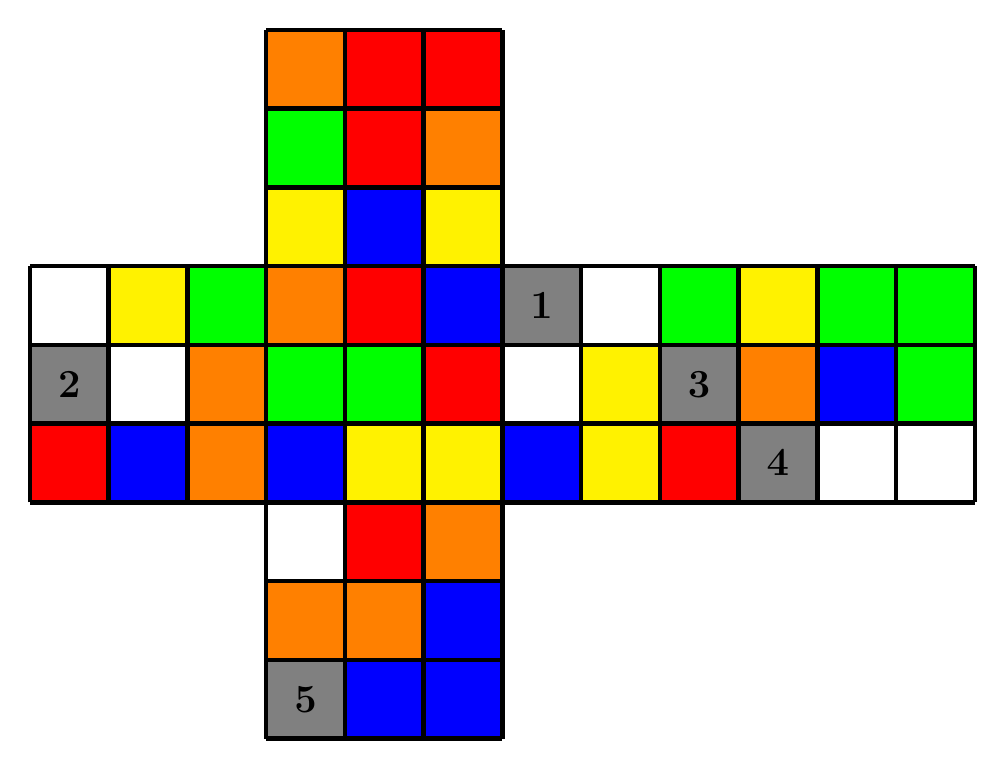
\begin{tikzpicture}[every node/.style={minimum size=1cm-\pgflinewidth, outer sep=0pt}]
\node[fill=orange] at (0.5,5.5) {};
\node[fill=red] at (1.5,5.5) {};
\node[fill=red] at (2.5,5.5) {};
\node[fill=green] at (0.5,4.5) {};
\node[fill=red] at (1.5,4.5) {};
\node[fill=orange] at (2.5,4.5) {};
\node[fill=yellow] at (0.5,3.5) {};
\node[fill=blue] at (1.5,3.5) {};
\node[fill=yellow] at (2.5,3.5) {};

\node[fill=white] at (-2.5,2.5) {};
\node[fill=yellow] at (-1.5,2.5) {};
\node[fill=green] at (-0.5,2.5) {};
\node[fill=orange] at (0.5,2.5) {};
\node[fill=red] at (1.5,2.5) {};
\node[fill=blue] at (2.5,2.5) {};
\node[fill=gray] at (3.5,2.5) {\Large \textbf 1};
\node[fill=white] at (4.5,2.5) {};
\node[fill=green] at (5.5,2.5) {};
\node[fill=yellow] at (6.5,2.5) {};
\node[fill=green] at (7.5,2.5) {};
\node[fill=green] at (8.5,2.5) {};

\node[fill=gray] at (-2.5,1.5) {\Large \textbf 2};
\node[fill=white] at (-1.5,1.5) {};
\node[fill=orange] at (-0.5,1.5) {};
\node[fill=green] at (0.5,1.5) {};
\node[fill=green] at (1.5,1.5) {};
\node[fill=red] at (2.5,1.5) {};
\node[fill=white] at (3.5,1.5) {};
\node[fill=yellow] at (4.5,1.5) {};
\node[fill=gray] at (5.5,1.5) {\Large \textbf 3};
\node[fill=orange] at (6.5,1.5) {};
\node[fill=blue] at (7.5,1.5) {};
\node[fill=green] at (8.5,1.5) {};

\node[fill=red] at (-2.5,0.5) {};
\node[fill=blue] at (-1.5,0.5) {};
\node[fill=orange] at (-0.5,0.5) {};
\node[fill=blue] at (0.5,0.5) {};
\node[fill=yellow] at (1.5,0.5) {};
\node[fill=yellow] at (2.5,0.5) {};
\node[fill=blue] at (3.5,0.5) {};
\node[fill=yellow] at (4.5,0.5) {};
\node[fill=red] at (5.5,0.5) {};
\node[fill=gray] at (6.5,0.5) {\Large \textbf 4};
\node[fill=white] at (7.5,0.5) {};
\node[fill=white] at (8.5,0.5) {};

\node[fill=white] at (0.5,-0.5) {};
\node[fill=red] at (1.5,-0.5) {};
\node[fill=orange] at (2.5,-0.5) {};
\node[fill=orange] at (0.5,-1.5) {};
\node[fill=orange] at (1.5,-1.5) {};
\node[fill=blue] at (2.5,-1.5) {};
\node[fill=gray] at (0.5,-2.5) {\Large \textbf 5};
\node[fill=blue] at (1.5,-2.5) {};
\node[fill=blue] at (2.5,-2.5) {};

\draw[step=1cm,color=black, ultra thick] (-3,0) grid (9,3);
\draw[step=1cm,color=black, ultra thick] (0,-3) grid (3,0);
\draw[step=1cm,color=black, ultra thick] (0,3) grid (3,6);
\end{tikzpicture}
\vspace{0.1cm}
\\
\noindent\normalsize \newtime  \textbf{Solution 12: L D' U' B' L2 B' R2 L' F2 L U2 F2 D U L2 F2 R' U' F2 U' Rw Uw }
\vspace{1cm}



{\noindent\Large  \newtime \textbf{No. 13\qquad Difficulty: $\bigstar$}}
\vspace{0.2cm}\\
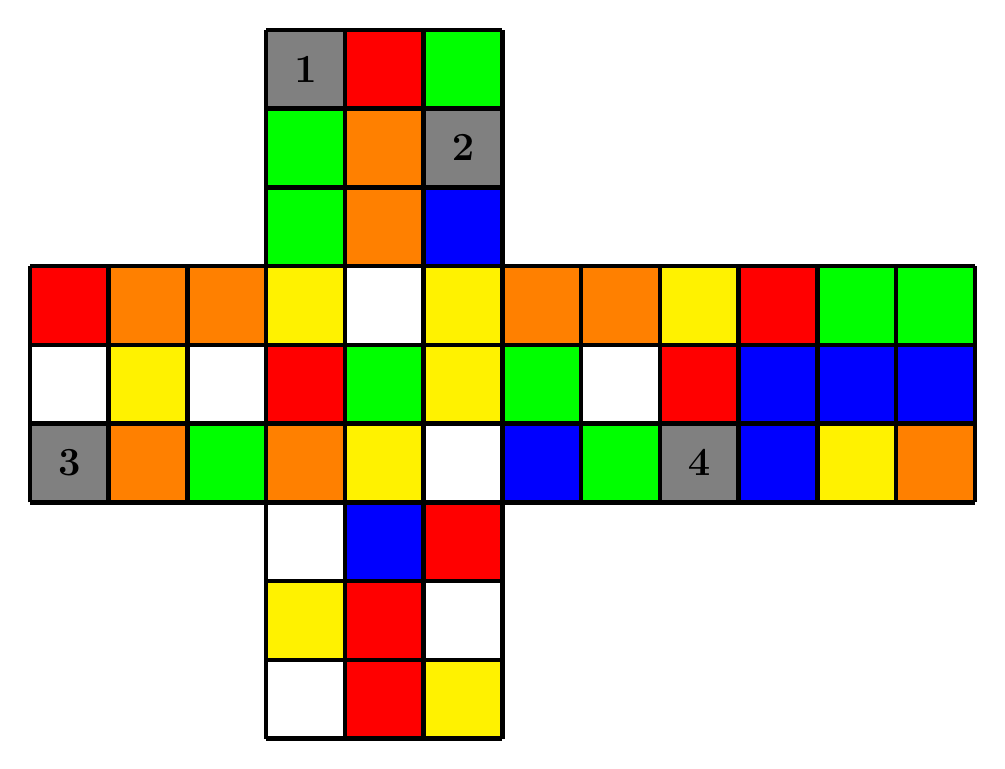
\begin{tikzpicture}[every node/.style={minimum size=1cm-\pgflinewidth, outer sep=0pt}]
\node[fill=gray] at (0.5,5.5) {\Large \textbf 1};
\node[fill=red] at (1.5,5.5) {};
\node[fill=green] at (2.5,5.5) {};
\node[fill=green] at (0.5,4.5) {};
\node[fill=orange] at (1.5,4.5) {};
\node[fill=gray] at (2.5,4.5) {\Large \textbf 2};
\node[fill=green] at (0.5,3.5) {};
\node[fill=orange] at (1.5,3.5) {};
\node[fill=blue] at (2.5,3.5) {};

\node[fill=red] at (-2.5,2.5) {};
\node[fill=orange] at (-1.5,2.5) {};
\node[fill=orange] at (-0.5,2.5) {};
\node[fill=yellow] at (0.5,2.5) {};
\node[fill=white] at (1.5,2.5) {};
\node[fill=yellow] at (2.5,2.5) {};
\node[fill=orange] at (3.5,2.5) {};
\node[fill=orange] at (4.5,2.5) {};
\node[fill=yellow] at (5.5,2.5) {};
\node[fill=red] at (6.5,2.5) {};
\node[fill=green] at (7.5,2.5) {};
\node[fill=green] at (8.5,2.5) {};

\node[fill=white] at (-2.5,1.5) {};
\node[fill=yellow] at (-1.5,1.5) {};
\node[fill=white] at (-0.5,1.5) {};
\node[fill=red] at (0.5,1.5) {};
\node[fill=green] at (1.5,1.5) {};
\node[fill=yellow] at (2.5,1.5) {};
\node[fill=green] at (3.5,1.5) {};
\node[fill=white] at (4.5,1.5) {};
\node[fill=red] at (5.5,1.5) {};
\node[fill=blue] at (6.5,1.5) {};
\node[fill=blue] at (7.5,1.5) {};
\node[fill=blue] at (8.5,1.5) {};

\node[fill=gray] at (-2.5,0.5) {\Large \textbf 3};
\node[fill=orange] at (-1.5,0.5) {};
\node[fill=green] at (-0.5,0.5) {};
\node[fill=orange] at (0.5,0.5) {};
\node[fill=yellow] at (1.5,0.5) {};
\node[fill=white] at (2.5,0.5) {};
\node[fill=blue] at (3.5,0.5) {};
\node[fill=green] at (4.5,0.5) {};
\node[fill=gray] at (5.5,0.5) {\Large \textbf 4};
\node[fill=blue] at (6.5,0.5) {};
\node[fill=yellow] at (7.5,0.5) {};
\node[fill=orange] at (8.5,0.5) {};

\node[fill=white] at (0.5,-0.5) {};
\node[fill=blue] at (1.5,-0.5) {};
\node[fill=red] at (2.5,-0.5) {};
\node[fill=yellow] at (0.5,-1.5) {};
\node[fill=red] at (1.5,-1.5) {};
\node[fill=white] at (2.5,-1.5) {};
\node[fill=white] at (0.5,-2.5) {};
\node[fill=red] at (1.5,-2.5) {};
\node[fill=yellow] at (2.5,-2.5) {};

\draw[step=1cm,color=black, ultra thick] (-3,0) grid (9,3);
\draw[step=1cm,color=black, ultra thick] (0,-3) grid (3,0);
\draw[step=1cm,color=black, ultra thick] (0,3) grid (3,6);
\end{tikzpicture}
\vspace{0.1cm}
\\
\noindent\normalsize \newtime  \textbf{Solution 13: F2 R' L U2 B' L' B2 R2 B U2 L2 U2 D2 B2 R F2 D2 U' L2 D Rw' Uw }
\vspace{1cm}



{\noindent\Large  \newtime \textbf{No. 14\qquad Difficulty: $\bigstar$}}
\vspace{0.2cm}\\
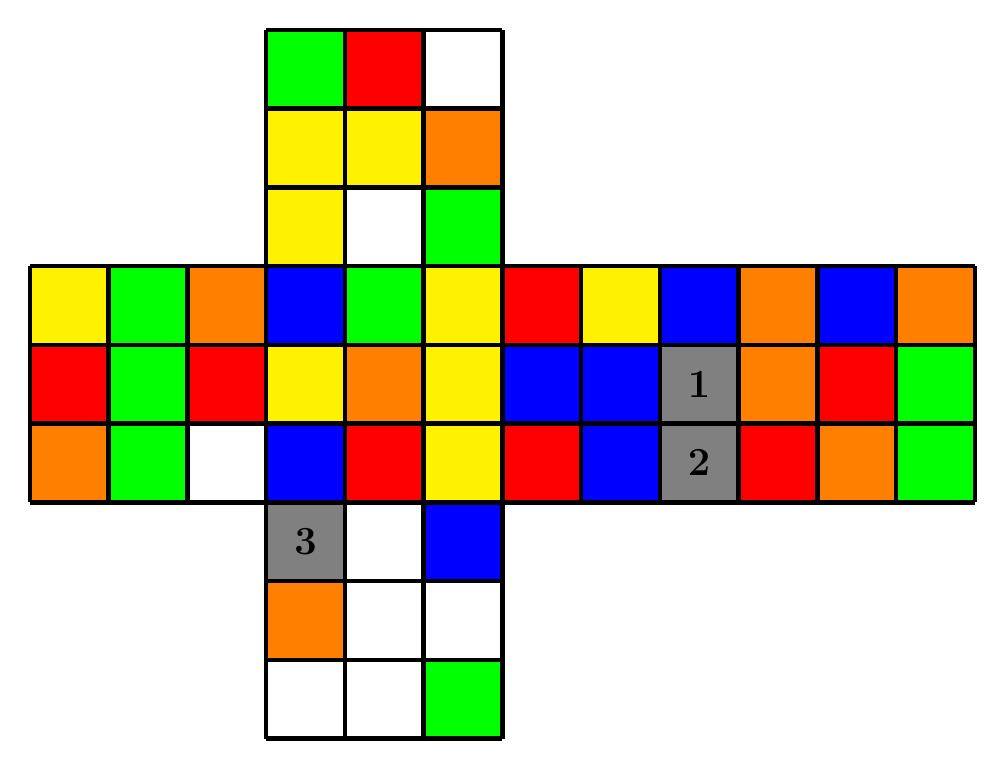
\begin{tikzpicture}[every node/.style={minimum size=1cm-\pgflinewidth, outer sep=0pt}]
\node[fill=green] at (0.5,5.5) {};
\node[fill=red] at (1.5,5.5) {};
\node[fill=white] at (2.5,5.5) {};
\node[fill=yellow] at (0.5,4.5) {};
\node[fill=yellow] at (1.5,4.5) {};
\node[fill=orange] at (2.5,4.5) {};
\node[fill=yellow] at (0.5,3.5) {};
\node[fill=white] at (1.5,3.5) {};
\node[fill=green] at (2.5,3.5) {};

\node[fill=yellow] at (-2.5,2.5) {};
\node[fill=green] at (-1.5,2.5) {};
\node[fill=orange] at (-0.5,2.5) {};
\node[fill=blue] at (0.5,2.5) {};
\node[fill=green] at (1.5,2.5) {};
\node[fill=yellow] at (2.5,2.5) {};
\node[fill=red] at (3.5,2.5) {};
\node[fill=yellow] at (4.5,2.5) {};
\node[fill=blue] at (5.5,2.5) {};
\node[fill=orange] at (6.5,2.5) {};
\node[fill=blue] at (7.5,2.5) {};
\node[fill=orange] at (8.5,2.5) {};

\node[fill=red] at (-2.5,1.5) {};
\node[fill=green] at (-1.5,1.5) {};
\node[fill=red] at (-0.5,1.5) {};
\node[fill=yellow] at (0.5,1.5) {};
\node[fill=orange] at (1.5,1.5) {};
\node[fill=yellow] at (2.5,1.5) {};
\node[fill=blue] at (3.5,1.5) {};
\node[fill=blue] at (4.5,1.5) {};
\node[fill=gray] at (5.5,1.5) {\Large \textbf 1};
\node[fill=orange] at (6.5,1.5) {};
\node[fill=red] at (7.5,1.5) {};
\node[fill=green] at (8.5,1.5) {};

\node[fill=orange] at (-2.5,0.5) {};
\node[fill=green] at (-1.5,0.5) {};
\node[fill=white] at (-0.5,0.5) {};
\node[fill=blue] at (0.5,0.5) {};
\node[fill=red] at (1.5,0.5) {};
\node[fill=yellow] at (2.5,0.5) {};
\node[fill=red] at (3.5,0.5) {};
\node[fill=blue] at (4.5,0.5) {};
\node[fill=gray] at (5.5,0.5) {\Large \textbf 2};
\node[fill=red] at (6.5,0.5) {};
\node[fill=orange] at (7.5,0.5) {};
\node[fill=green] at (8.5,0.5) {};

\node[fill=gray] at (0.5,-0.5) {\Large \textbf 3};
\node[fill=white] at (1.5,-0.5) {};
\node[fill=blue] at (2.5,-0.5) {};
\node[fill=orange] at (0.5,-1.5) {};
\node[fill=white] at (1.5,-1.5) {};
\node[fill=white] at (2.5,-1.5) {};
\node[fill=white] at (0.5,-2.5) {};
\node[fill=white] at (1.5,-2.5) {};
\node[fill=green] at (2.5,-2.5) {};

\draw[step=1cm,color=black, ultra thick] (-3,0) grid (9,3);
\draw[step=1cm,color=black, ultra thick] (0,-3) grid (3,0);
\draw[step=1cm,color=black, ultra thick] (0,3) grid (3,6);
\end{tikzpicture}
\vspace{0.1cm}
\\
\noindent\normalsize \newtime  \textbf{Solution 14: F2 L2 D2 F2 L B' R D2 U R B' R U L2 B2 L' F L F' R Uw2 }
\vspace{1cm}



{\noindent\Large  \newtime \textbf{No. 15\qquad Difficulty: $\bigstar$}}
\vspace{0.2cm}\\
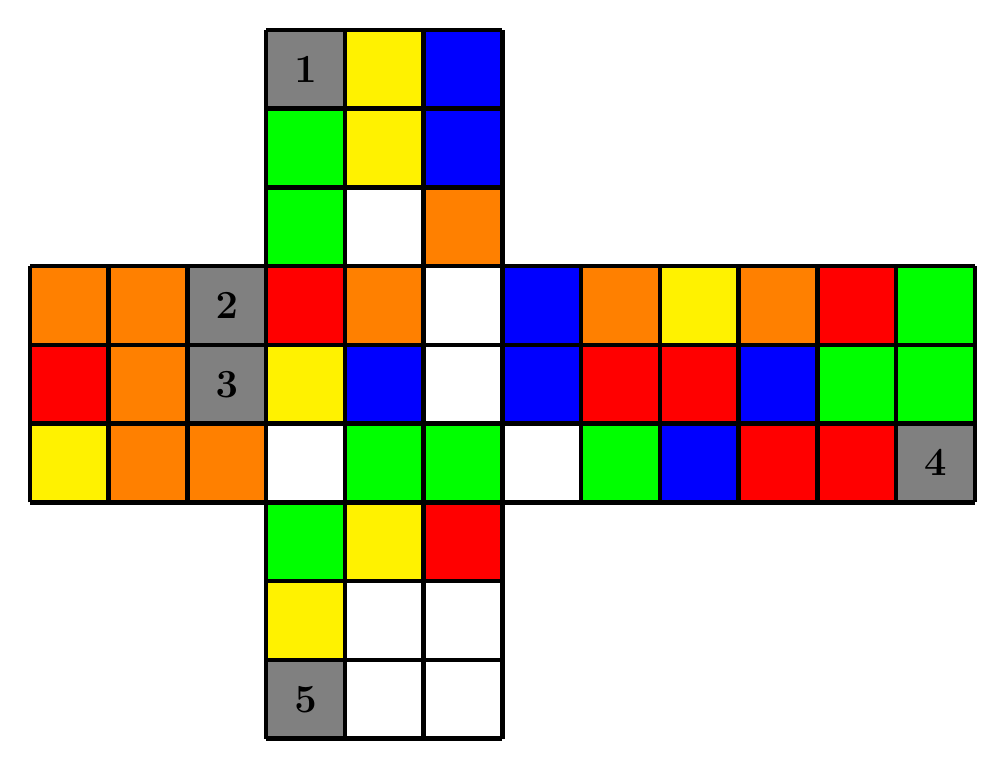
\begin{tikzpicture}[every node/.style={minimum size=1cm-\pgflinewidth, outer sep=0pt}]
\node[fill=gray] at (0.5,5.5) {\Large \textbf 1};
\node[fill=yellow] at (1.5,5.5) {};
\node[fill=blue] at (2.5,5.5) {};
\node[fill=green] at (0.5,4.5) {};
\node[fill=yellow] at (1.5,4.5) {};
\node[fill=blue] at (2.5,4.5) {};
\node[fill=green] at (0.5,3.5) {};
\node[fill=white] at (1.5,3.5) {};
\node[fill=orange] at (2.5,3.5) {};

\node[fill=orange] at (-2.5,2.5) {};
\node[fill=orange] at (-1.5,2.5) {};
\node[fill=gray] at (-0.5,2.5) {\Large \textbf 2};
\node[fill=red] at (0.5,2.5) {};
\node[fill=orange] at (1.5,2.5) {};
\node[fill=white] at (2.5,2.5) {};
\node[fill=blue] at (3.5,2.5) {};
\node[fill=orange] at (4.5,2.5) {};
\node[fill=yellow] at (5.5,2.5) {};
\node[fill=orange] at (6.5,2.5) {};
\node[fill=red] at (7.5,2.5) {};
\node[fill=green] at (8.5,2.5) {};

\node[fill=red] at (-2.5,1.5) {};
\node[fill=orange] at (-1.5,1.5) {};
\node[fill=gray] at (-0.5,1.5) {\Large \textbf 3};
\node[fill=yellow] at (0.5,1.5) {};
\node[fill=blue] at (1.5,1.5) {};
\node[fill=white] at (2.5,1.5) {};
\node[fill=blue] at (3.5,1.5) {};
\node[fill=red] at (4.5,1.5) {};
\node[fill=red] at (5.5,1.5) {};
\node[fill=blue] at (6.5,1.5) {};
\node[fill=green] at (7.5,1.5) {};
\node[fill=green] at (8.5,1.5) {};

\node[fill=yellow] at (-2.5,0.5) {};
\node[fill=orange] at (-1.5,0.5) {};
\node[fill=orange] at (-0.5,0.5) {};
\node[fill=white] at (0.5,0.5) {};
\node[fill=green] at (1.5,0.5) {};
\node[fill=green] at (2.5,0.5) {};
\node[fill=white] at (3.5,0.5) {};
\node[fill=green] at (4.5,0.5) {};
\node[fill=blue] at (5.5,0.5) {};
\node[fill=red] at (6.5,0.5) {};
\node[fill=red] at (7.5,0.5) {};
\node[fill=gray] at (8.5,0.5) {\Large \textbf 4};

\node[fill=green] at (0.5,-0.5) {};
\node[fill=yellow] at (1.5,-0.5) {};
\node[fill=red] at (2.5,-0.5) {};
\node[fill=yellow] at (0.5,-1.5) {};
\node[fill=white] at (1.5,-1.5) {};
\node[fill=white] at (2.5,-1.5) {};
\node[fill=gray] at (0.5,-2.5) {\Large \textbf 5};
\node[fill=white] at (1.5,-2.5) {};
\node[fill=white] at (2.5,-2.5) {};

\draw[step=1cm,color=black, ultra thick] (-3,0) grid (9,3);
\draw[step=1cm,color=black, ultra thick] (0,-3) grid (3,0);
\draw[step=1cm,color=black, ultra thick] (0,3) grid (3,6);
\end{tikzpicture}
\vspace{0.1cm}
\\
\noindent\normalsize \newtime  \textbf{Solution 15: B F L2 F' L2 F U2 F B' D F2 B' U2 B L2 D' B' D R2 D' Uw' }
\vspace{1cm}



{\noindent\Large  \newtime \textbf{No. 16\qquad Difficulty: $\bigstar$}}
\vspace{0.2cm}\\
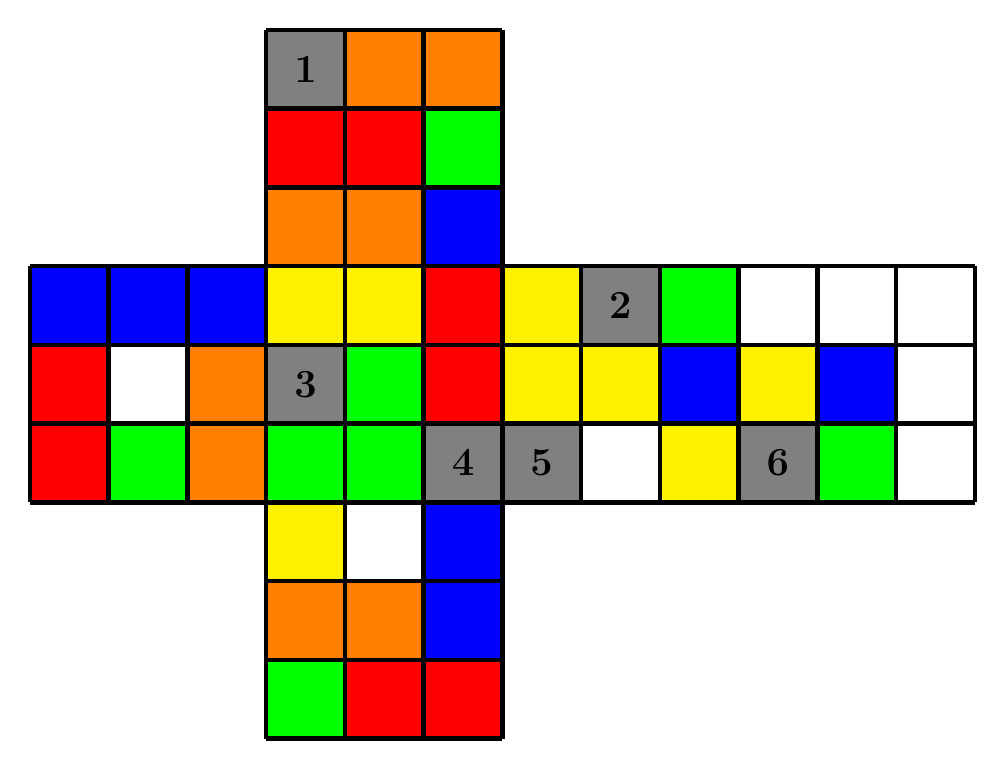
\begin{tikzpicture}[every node/.style={minimum size=1cm-\pgflinewidth, outer sep=0pt}]
\node[fill=gray] at (0.5,5.5) {\Large \textbf 1};
\node[fill=orange] at (1.5,5.5) {};
\node[fill=orange] at (2.5,5.5) {};
\node[fill=red] at (0.5,4.5) {};
\node[fill=red] at (1.5,4.5) {};
\node[fill=green] at (2.5,4.5) {};
\node[fill=orange] at (0.5,3.5) {};
\node[fill=orange] at (1.5,3.5) {};
\node[fill=blue] at (2.5,3.5) {};

\node[fill=blue] at (-2.5,2.5) {};
\node[fill=blue] at (-1.5,2.5) {};
\node[fill=blue] at (-0.5,2.5) {};
\node[fill=yellow] at (0.5,2.5) {};
\node[fill=yellow] at (1.5,2.5) {};
\node[fill=red] at (2.5,2.5) {};
\node[fill=yellow] at (3.5,2.5) {};
\node[fill=gray] at (4.5,2.5) {\Large \textbf 2};
\node[fill=green] at (5.5,2.5) {};
\node[fill=white] at (6.5,2.5) {};
\node[fill=white] at (7.5,2.5) {};
\node[fill=white] at (8.5,2.5) {};

\node[fill=red] at (-2.5,1.5) {};
\node[fill=white] at (-1.5,1.5) {};
\node[fill=orange] at (-0.5,1.5) {};
\node[fill=gray] at (0.5,1.5) {\Large \textbf 3};
\node[fill=green] at (1.5,1.5) {};
\node[fill=red] at (2.5,1.5) {};
\node[fill=yellow] at (3.5,1.5) {};
\node[fill=yellow] at (4.5,1.5) {};
\node[fill=blue] at (5.5,1.5) {};
\node[fill=yellow] at (6.5,1.5) {};
\node[fill=blue] at (7.5,1.5) {};
\node[fill=white] at (8.5,1.5) {};

\node[fill=red] at (-2.5,0.5) {};
\node[fill=green] at (-1.5,0.5) {};
\node[fill=orange] at (-0.5,0.5) {};
\node[fill=green] at (0.5,0.5) {};
\node[fill=green] at (1.5,0.5) {};
\node[fill=gray] at (2.5,0.5) {\Large \textbf 4};
\node[fill=gray] at (3.5,0.5) {\Large \textbf 5};
\node[fill=white] at (4.5,0.5) {};
\node[fill=yellow] at (5.5,0.5) {};
\node[fill=gray] at (6.5,0.5) {\Large \textbf 6};
\node[fill=green] at (7.5,0.5) {};
\node[fill=white] at (8.5,0.5) {};

\node[fill=yellow] at (0.5,-0.5) {};
\node[fill=white] at (1.5,-0.5) {};
\node[fill=blue] at (2.5,-0.5) {};
\node[fill=orange] at (0.5,-1.5) {};
\node[fill=orange] at (1.5,-1.5) {};
\node[fill=blue] at (2.5,-1.5) {};
\node[fill=green] at (0.5,-2.5) {};
\node[fill=red] at (1.5,-2.5) {};
\node[fill=red] at (2.5,-2.5) {};

\draw[step=1cm,color=black, ultra thick] (-3,0) grid (9,3);
\draw[step=1cm,color=black, ultra thick] (0,-3) grid (3,0);
\draw[step=1cm,color=black, ultra thick] (0,3) grid (3,6);
\end{tikzpicture}
\vspace{0.1cm}
\\
\noindent\normalsize \newtime  \textbf{Solution 16: B' R' B' R' U F2 B R2 L' U D' U B2 F R2 U' B R D2 L' Rw Uw }
\vspace{1cm}



{\noindent\Large  \newtime \textbf{No. 17\qquad Difficulty: $\bigstar$}}
\vspace{0.2cm}\\
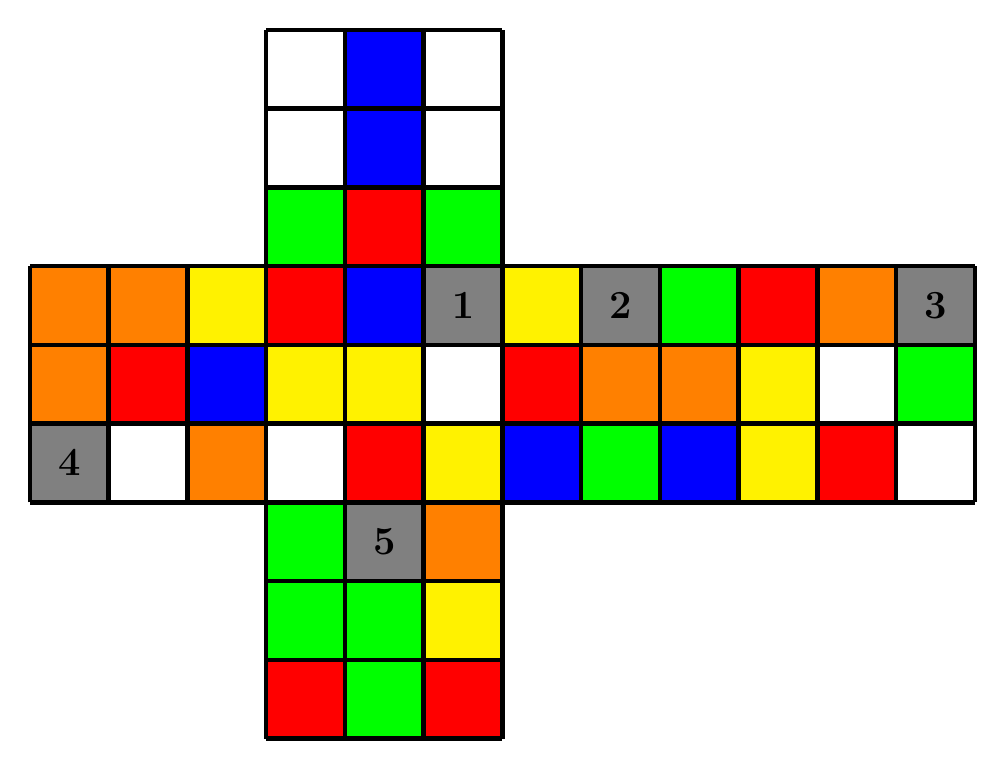
\begin{tikzpicture}[every node/.style={minimum size=1cm-\pgflinewidth, outer sep=0pt}]
\node[fill=white] at (0.5,5.5) {};
\node[fill=blue] at (1.5,5.5) {};
\node[fill=white] at (2.5,5.5) {};
\node[fill=white] at (0.5,4.5) {};
\node[fill=blue] at (1.5,4.5) {};
\node[fill=white] at (2.5,4.5) {};
\node[fill=green] at (0.5,3.5) {};
\node[fill=red] at (1.5,3.5) {};
\node[fill=green] at (2.5,3.5) {};

\node[fill=orange] at (-2.5,2.5) {};
\node[fill=orange] at (-1.5,2.5) {};
\node[fill=yellow] at (-0.5,2.5) {};
\node[fill=red] at (0.5,2.5) {};
\node[fill=blue] at (1.5,2.5) {};
\node[fill=gray] at (2.5,2.5) {\Large \textbf 1};
\node[fill=yellow] at (3.5,2.5) {};
\node[fill=gray] at (4.5,2.5) {\Large \textbf 2};
\node[fill=green] at (5.5,2.5) {};
\node[fill=red] at (6.5,2.5) {};
\node[fill=orange] at (7.5,2.5) {};
\node[fill=gray] at (8.5,2.5) {\Large \textbf 3};

\node[fill=orange] at (-2.5,1.5) {};
\node[fill=red] at (-1.5,1.5) {};
\node[fill=blue] at (-0.5,1.5) {};
\node[fill=yellow] at (0.5,1.5) {};
\node[fill=yellow] at (1.5,1.5) {};
\node[fill=white] at (2.5,1.5) {};
\node[fill=red] at (3.5,1.5) {};
\node[fill=orange] at (4.5,1.5) {};
\node[fill=orange] at (5.5,1.5) {};
\node[fill=yellow] at (6.5,1.5) {};
\node[fill=white] at (7.5,1.5) {};
\node[fill=green] at (8.5,1.5) {};

\node[fill=gray] at (-2.5,0.5) {\Large \textbf 4};
\node[fill=white] at (-1.5,0.5) {};
\node[fill=orange] at (-0.5,0.5) {};
\node[fill=white] at (0.5,0.5) {};
\node[fill=red] at (1.5,0.5) {};
\node[fill=yellow] at (2.5,0.5) {};
\node[fill=blue] at (3.5,0.5) {};
\node[fill=green] at (4.5,0.5) {};
\node[fill=blue] at (5.5,0.5) {};
\node[fill=yellow] at (6.5,0.5) {};
\node[fill=red] at (7.5,0.5) {};
\node[fill=white] at (8.5,0.5) {};

\node[fill=green] at (0.5,-0.5) {};
\node[fill=gray] at (1.5,-0.5) {\Large \textbf 5};
\node[fill=orange] at (2.5,-0.5) {};
\node[fill=green] at (0.5,-1.5) {};
\node[fill=green] at (1.5,-1.5) {};
\node[fill=yellow] at (2.5,-1.5) {};
\node[fill=red] at (0.5,-2.5) {};
\node[fill=green] at (1.5,-2.5) {};
\node[fill=red] at (2.5,-2.5) {};

\draw[step=1cm,color=black, ultra thick] (-3,0) grid (9,3);
\draw[step=1cm,color=black, ultra thick] (0,-3) grid (3,0);
\draw[step=1cm,color=black, ultra thick] (0,3) grid (3,6);
\end{tikzpicture}
\vspace{0.1cm}
\\
\noindent\normalsize \newtime  \textbf{Solution 17: F' R' D2 F2 L' D2 F2 B' R2 D2 R F' B2 U2 L2 B' R' L F' U' Fw Uw }
\vspace{1cm}



{\noindent\Large  \newtime \textbf{No. 18\qquad Difficulty: $\bigstar$}}
\vspace{0.2cm}\\
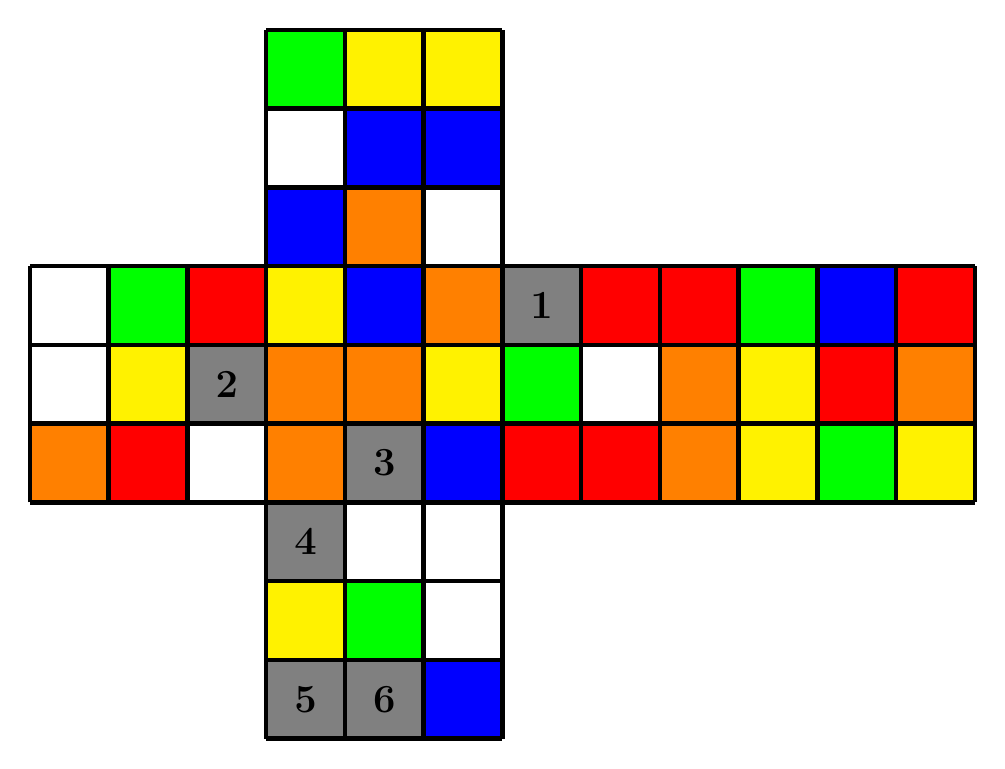
\begin{tikzpicture}[every node/.style={minimum size=1cm-\pgflinewidth, outer sep=0pt}]
\node[fill=green] at (0.5,5.5) {};
\node[fill=yellow] at (1.5,5.5) {};
\node[fill=yellow] at (2.5,5.5) {};
\node[fill=white] at (0.5,4.5) {};
\node[fill=blue] at (1.5,4.5) {};
\node[fill=blue] at (2.5,4.5) {};
\node[fill=blue] at (0.5,3.5) {};
\node[fill=orange] at (1.5,3.5) {};
\node[fill=white] at (2.5,3.5) {};

\node[fill=white] at (-2.5,2.5) {};
\node[fill=green] at (-1.5,2.5) {};
\node[fill=red] at (-0.5,2.5) {};
\node[fill=yellow] at (0.5,2.5) {};
\node[fill=blue] at (1.5,2.5) {};
\node[fill=orange] at (2.5,2.5) {};
\node[fill=gray] at (3.5,2.5) {\Large \textbf 1};
\node[fill=red] at (4.5,2.5) {};
\node[fill=red] at (5.5,2.5) {};
\node[fill=green] at (6.5,2.5) {};
\node[fill=blue] at (7.5,2.5) {};
\node[fill=red] at (8.5,2.5) {};

\node[fill=white] at (-2.5,1.5) {};
\node[fill=yellow] at (-1.5,1.5) {};
\node[fill=gray] at (-0.5,1.5) {\Large \textbf 2};
\node[fill=orange] at (0.5,1.5) {};
\node[fill=orange] at (1.5,1.5) {};
\node[fill=yellow] at (2.5,1.5) {};
\node[fill=green] at (3.5,1.5) {};
\node[fill=white] at (4.5,1.5) {};
\node[fill=orange] at (5.5,1.5) {};
\node[fill=yellow] at (6.5,1.5) {};
\node[fill=red] at (7.5,1.5) {};
\node[fill=orange] at (8.5,1.5) {};

\node[fill=orange] at (-2.5,0.5) {};
\node[fill=red] at (-1.5,0.5) {};
\node[fill=white] at (-0.5,0.5) {};
\node[fill=orange] at (0.5,0.5) {};
\node[fill=gray] at (1.5,0.5) {\Large \textbf 3};
\node[fill=blue] at (2.5,0.5) {};
\node[fill=red] at (3.5,0.5) {};
\node[fill=red] at (4.5,0.5) {};
\node[fill=orange] at (5.5,0.5) {};
\node[fill=yellow] at (6.5,0.5) {};
\node[fill=green] at (7.5,0.5) {};
\node[fill=yellow] at (8.5,0.5) {};

\node[fill=gray] at (0.5,-0.5) {\Large \textbf 4};
\node[fill=white] at (1.5,-0.5) {};
\node[fill=white] at (2.5,-0.5) {};
\node[fill=yellow] at (0.5,-1.5) {};
\node[fill=green] at (1.5,-1.5) {};
\node[fill=white] at (2.5,-1.5) {};
\node[fill=gray] at (0.5,-2.5) {\Large \textbf 5};
\node[fill=gray] at (1.5,-2.5) {\Large \textbf 6};
\node[fill=blue] at (2.5,-2.5) {};

\draw[step=1cm,color=black, ultra thick] (-3,0) grid (9,3);
\draw[step=1cm,color=black, ultra thick] (0,-3) grid (3,0);
\draw[step=1cm,color=black, ultra thick] (0,3) grid (3,6);
\end{tikzpicture}
\vspace{0.1cm}
\\
\noindent\normalsize \newtime  \textbf{Solution 18: R2 D' U2 L' U' B2 U' F' B D F' R L F R D2 U' B F2 R' Fw Uw2 }
\vspace{1cm}



{\noindent\Large  \newtime \textbf{No. 19\qquad Difficulty: $\bigstar$}}
\vspace{0.2cm}\\
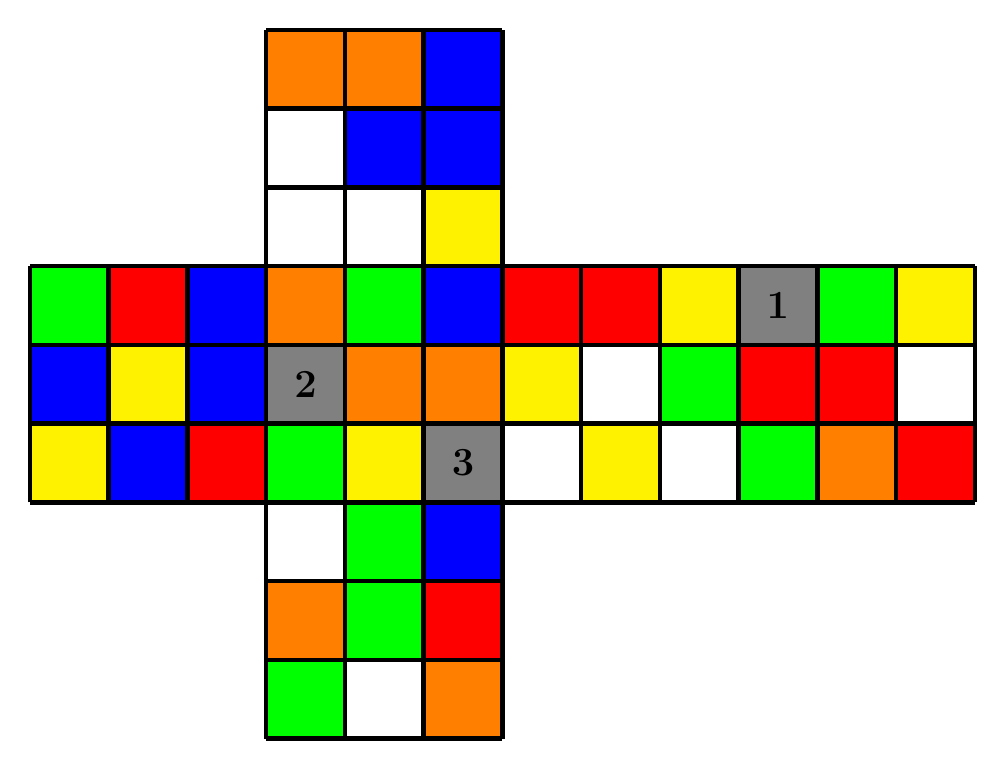
\begin{tikzpicture}[every node/.style={minimum size=1cm-\pgflinewidth, outer sep=0pt}]
\node[fill=orange] at (0.5,5.5) {};
\node[fill=orange] at (1.5,5.5) {};
\node[fill=blue] at (2.5,5.5) {};
\node[fill=white] at (0.5,4.5) {};
\node[fill=blue] at (1.5,4.5) {};
\node[fill=blue] at (2.5,4.5) {};
\node[fill=white] at (0.5,3.5) {};
\node[fill=white] at (1.5,3.5) {};
\node[fill=yellow] at (2.5,3.5) {};

\node[fill=green] at (-2.5,2.5) {};
\node[fill=red] at (-1.5,2.5) {};
\node[fill=blue] at (-0.5,2.5) {};
\node[fill=orange] at (0.5,2.5) {};
\node[fill=green] at (1.5,2.5) {};
\node[fill=blue] at (2.5,2.5) {};
\node[fill=red] at (3.5,2.5) {};
\node[fill=red] at (4.5,2.5) {};
\node[fill=yellow] at (5.5,2.5) {};
\node[fill=gray] at (6.5,2.5) {\Large \textbf 1};
\node[fill=green] at (7.5,2.5) {};
\node[fill=yellow] at (8.5,2.5) {};

\node[fill=blue] at (-2.5,1.5) {};
\node[fill=yellow] at (-1.5,1.5) {};
\node[fill=blue] at (-0.5,1.5) {};
\node[fill=gray] at (0.5,1.5) {\Large \textbf 2};
\node[fill=orange] at (1.5,1.5) {};
\node[fill=orange] at (2.5,1.5) {};
\node[fill=yellow] at (3.5,1.5) {};
\node[fill=white] at (4.5,1.5) {};
\node[fill=green] at (5.5,1.5) {};
\node[fill=red] at (6.5,1.5) {};
\node[fill=red] at (7.5,1.5) {};
\node[fill=white] at (8.5,1.5) {};

\node[fill=yellow] at (-2.5,0.5) {};
\node[fill=blue] at (-1.5,0.5) {};
\node[fill=red] at (-0.5,0.5) {};
\node[fill=green] at (0.5,0.5) {};
\node[fill=yellow] at (1.5,0.5) {};
\node[fill=gray] at (2.5,0.5) {\Large \textbf 3};
\node[fill=white] at (3.5,0.5) {};
\node[fill=yellow] at (4.5,0.5) {};
\node[fill=white] at (5.5,0.5) {};
\node[fill=green] at (6.5,0.5) {};
\node[fill=orange] at (7.5,0.5) {};
\node[fill=red] at (8.5,0.5) {};

\node[fill=white] at (0.5,-0.5) {};
\node[fill=green] at (1.5,-0.5) {};
\node[fill=blue] at (2.5,-0.5) {};
\node[fill=orange] at (0.5,-1.5) {};
\node[fill=green] at (1.5,-1.5) {};
\node[fill=red] at (2.5,-1.5) {};
\node[fill=green] at (0.5,-2.5) {};
\node[fill=white] at (1.5,-2.5) {};
\node[fill=orange] at (2.5,-2.5) {};

\draw[step=1cm,color=black, ultra thick] (-3,0) grid (9,3);
\draw[step=1cm,color=black, ultra thick] (0,-3) grid (3,0);
\draw[step=1cm,color=black, ultra thick] (0,3) grid (3,6);
\end{tikzpicture}
\vspace{0.1cm}
\\
\noindent\normalsize \newtime  \textbf{Solution 19: L' U2 L D' B' D' L R2 D2 U' B' U F' R' U D2 R2 U2 B L2 Fw Uw2 }
\vspace{1cm}



{\noindent\Large  \newtime \textbf{No. 20\qquad Difficulty: $\bigstar$}}
\vspace{0.2cm}\\
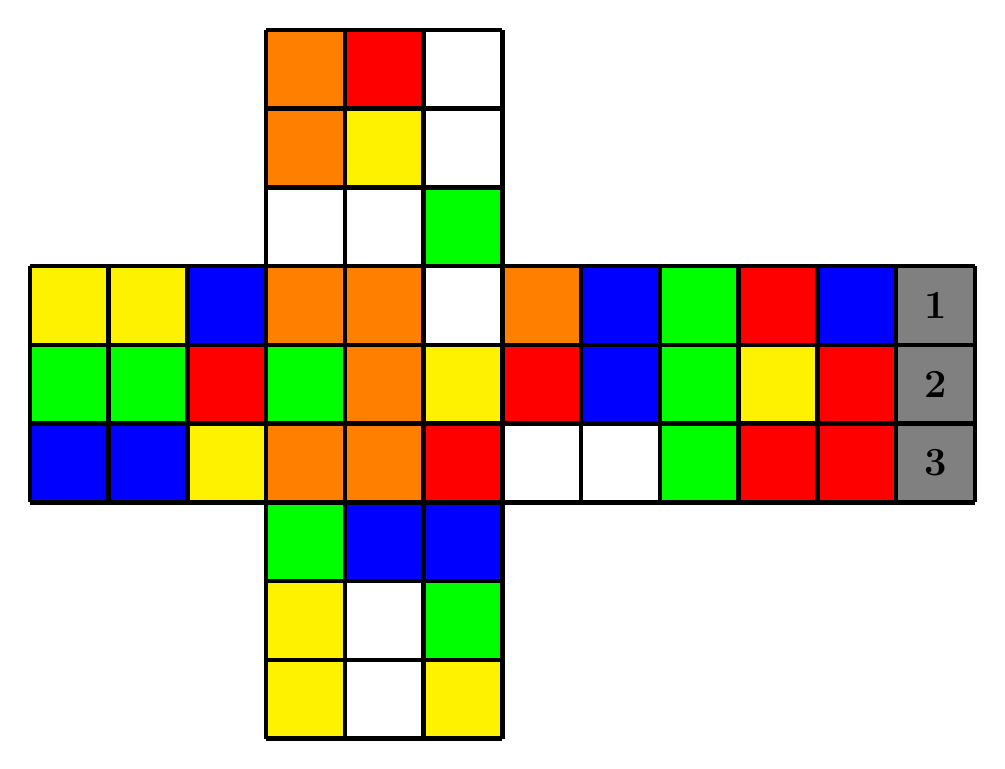
\begin{tikzpicture}[every node/.style={minimum size=1cm-\pgflinewidth, outer sep=0pt}]
\node[fill=orange] at (0.5,5.5) {};
\node[fill=red] at (1.5,5.5) {};
\node[fill=white] at (2.5,5.5) {};
\node[fill=orange] at (0.5,4.5) {};
\node[fill=yellow] at (1.5,4.5) {};
\node[fill=white] at (2.5,4.5) {};
\node[fill=white] at (0.5,3.5) {};
\node[fill=white] at (1.5,3.5) {};
\node[fill=green] at (2.5,3.5) {};

\node[fill=yellow] at (-2.5,2.5) {};
\node[fill=yellow] at (-1.5,2.5) {};
\node[fill=blue] at (-0.5,2.5) {};
\node[fill=orange] at (0.5,2.5) {};
\node[fill=orange] at (1.5,2.5) {};
\node[fill=white] at (2.5,2.5) {};
\node[fill=orange] at (3.5,2.5) {};
\node[fill=blue] at (4.5,2.5) {};
\node[fill=green] at (5.5,2.5) {};
\node[fill=red] at (6.5,2.5) {};
\node[fill=blue] at (7.5,2.5) {};
\node[fill=gray] at (8.5,2.5) {\Large \textbf 1};

\node[fill=green] at (-2.5,1.5) {};
\node[fill=green] at (-1.5,1.5) {};
\node[fill=red] at (-0.5,1.5) {};
\node[fill=green] at (0.5,1.5) {};
\node[fill=orange] at (1.5,1.5) {};
\node[fill=yellow] at (2.5,1.5) {};
\node[fill=red] at (3.5,1.5) {};
\node[fill=blue] at (4.5,1.5) {};
\node[fill=green] at (5.5,1.5) {};
\node[fill=yellow] at (6.5,1.5) {};
\node[fill=red] at (7.5,1.5) {};
\node[fill=gray] at (8.5,1.5) {\Large \textbf 2};

\node[fill=blue] at (-2.5,0.5) {};
\node[fill=blue] at (-1.5,0.5) {};
\node[fill=yellow] at (-0.5,0.5) {};
\node[fill=orange] at (0.5,0.5) {};
\node[fill=orange] at (1.5,0.5) {};
\node[fill=red] at (2.5,0.5) {};
\node[fill=white] at (3.5,0.5) {};
\node[fill=white] at (4.5,0.5) {};
\node[fill=green] at (5.5,0.5) {};
\node[fill=red] at (6.5,0.5) {};
\node[fill=red] at (7.5,0.5) {};
\node[fill=gray] at (8.5,0.5) {\Large \textbf 3};

\node[fill=green] at (0.5,-0.5) {};
\node[fill=blue] at (1.5,-0.5) {};
\node[fill=blue] at (2.5,-0.5) {};
\node[fill=yellow] at (0.5,-1.5) {};
\node[fill=white] at (1.5,-1.5) {};
\node[fill=green] at (2.5,-1.5) {};
\node[fill=yellow] at (0.5,-2.5) {};
\node[fill=white] at (1.5,-2.5) {};
\node[fill=yellow] at (2.5,-2.5) {};

\draw[step=1cm,color=black, ultra thick] (-3,0) grid (9,3);
\draw[step=1cm,color=black, ultra thick] (0,-3) grid (3,0);
\draw[step=1cm,color=black, ultra thick] (0,3) grid (3,6);
\end{tikzpicture}
\vspace{0.1cm}
\\
\noindent\normalsize \newtime  \textbf{Solution 20: U2 R2 L2 B L' D' L U2 L2 U L U B' L2 F R F' B2 L2 D' Uw2 }
\vspace{1cm}



{\noindent\Large  \newtime \textbf{No. 21\qquad Difficulty: $\bigstar\bigstar$}}
\vspace{0.2cm}\\
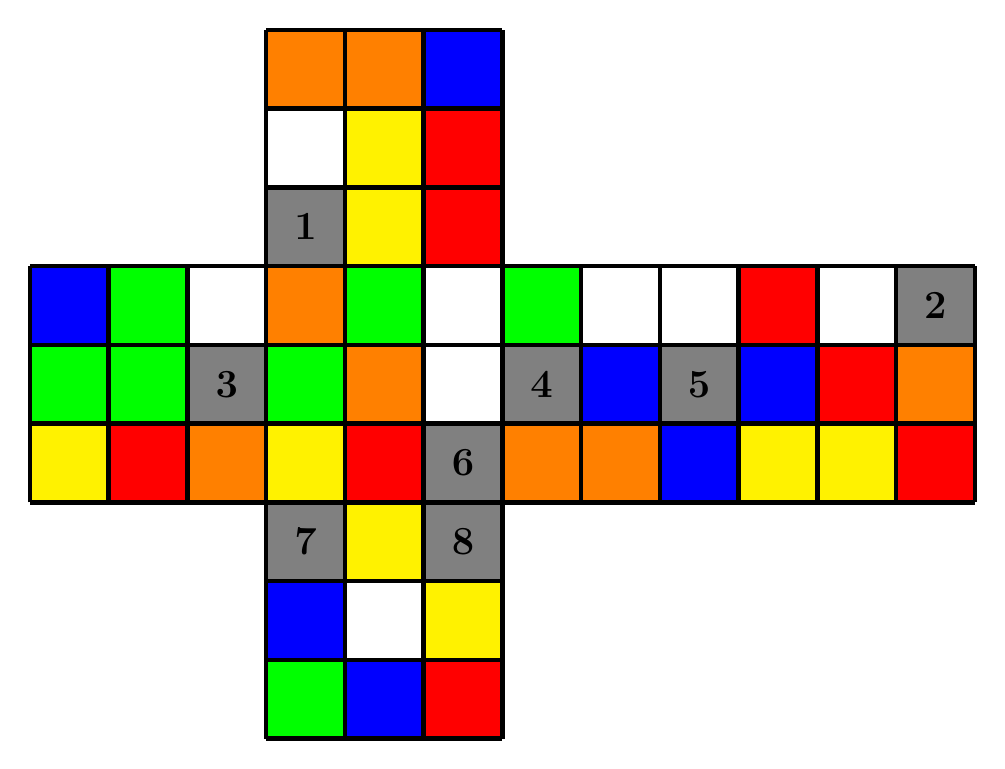
\begin{tikzpicture}[every node/.style={minimum size=1cm-\pgflinewidth, outer sep=0pt}]
\node[fill=orange] at (0.5,5.5) {};
\node[fill=orange] at (1.5,5.5) {};
\node[fill=blue] at (2.5,5.5) {};
\node[fill=white] at (0.5,4.5) {};
\node[fill=yellow] at (1.5,4.5) {};
\node[fill=red] at (2.5,4.5) {};
\node[fill=gray] at (0.5,3.5) {\Large \textbf 1};
\node[fill=yellow] at (1.5,3.5) {};
\node[fill=red] at (2.5,3.5) {};

\node[fill=blue] at (-2.5,2.5) {};
\node[fill=green] at (-1.5,2.5) {};
\node[fill=white] at (-0.5,2.5) {};
\node[fill=orange] at (0.5,2.5) {};
\node[fill=green] at (1.5,2.5) {};
\node[fill=white] at (2.5,2.5) {};
\node[fill=green] at (3.5,2.5) {};
\node[fill=white] at (4.5,2.5) {};
\node[fill=white] at (5.5,2.5) {};
\node[fill=red] at (6.5,2.5) {};
\node[fill=white] at (7.5,2.5) {};
\node[fill=gray] at (8.5,2.5) {\Large \textbf 2};

\node[fill=green] at (-2.5,1.5) {};
\node[fill=green] at (-1.5,1.5) {};
\node[fill=gray] at (-0.5,1.5) {\Large \textbf 3};
\node[fill=green] at (0.5,1.5) {};
\node[fill=orange] at (1.5,1.5) {};
\node[fill=white] at (2.5,1.5) {};
\node[fill=gray] at (3.5,1.5) {\Large \textbf 4};
\node[fill=blue] at (4.5,1.5) {};
\node[fill=gray] at (5.5,1.5) {\Large \textbf 5};
\node[fill=blue] at (6.5,1.5) {};
\node[fill=red] at (7.5,1.5) {};
\node[fill=orange] at (8.5,1.5) {};

\node[fill=yellow] at (-2.5,0.5) {};
\node[fill=red] at (-1.5,0.5) {};
\node[fill=orange] at (-0.5,0.5) {};
\node[fill=yellow] at (0.5,0.5) {};
\node[fill=red] at (1.5,0.5) {};
\node[fill=gray] at (2.5,0.5) {\Large \textbf 6};
\node[fill=orange] at (3.5,0.5) {};
\node[fill=orange] at (4.5,0.5) {};
\node[fill=blue] at (5.5,0.5) {};
\node[fill=yellow] at (6.5,0.5) {};
\node[fill=yellow] at (7.5,0.5) {};
\node[fill=red] at (8.5,0.5) {};

\node[fill=gray] at (0.5,-0.5) {\Large \textbf 7};
\node[fill=yellow] at (1.5,-0.5) {};
\node[fill=gray] at (2.5,-0.5) {\Large \textbf 8};
\node[fill=blue] at (0.5,-1.5) {};
\node[fill=white] at (1.5,-1.5) {};
\node[fill=yellow] at (2.5,-1.5) {};
\node[fill=green] at (0.5,-2.5) {};
\node[fill=blue] at (1.5,-2.5) {};
\node[fill=red] at (2.5,-2.5) {};

\draw[step=1cm,color=black, ultra thick] (-3,0) grid (9,3);
\draw[step=1cm,color=black, ultra thick] (0,-3) grid (3,0);
\draw[step=1cm,color=black, ultra thick] (0,3) grid (3,6);
\end{tikzpicture}
\vspace{0.1cm}
\\
\noindent\normalsize \newtime  \textbf{Solution 21: B2 F' U L R' B2 L2 B' U' F2 L' U' B' U R2 F' U2 R' F' D' Uw2 }
\vspace{1cm}



{\noindent\Large  \newtime \textbf{No. 22\qquad Difficulty: $\bigstar\bigstar$}}
\vspace{0.2cm}\\
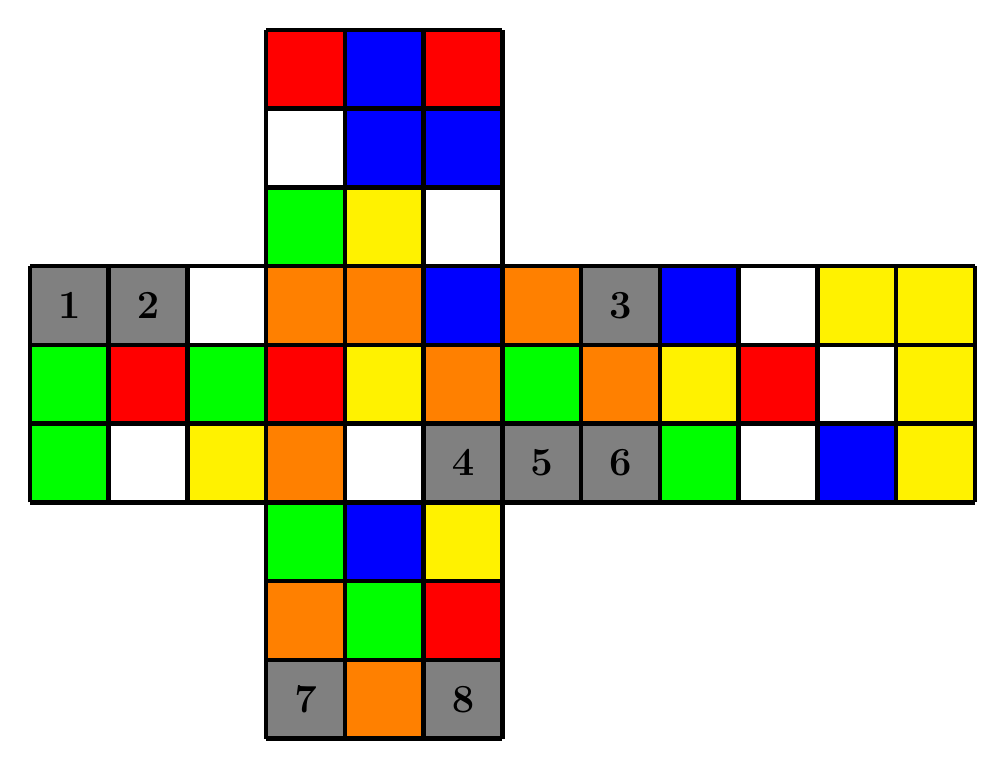
\begin{tikzpicture}[every node/.style={minimum size=1cm-\pgflinewidth, outer sep=0pt}]
\node[fill=red] at (0.5,5.5) {};
\node[fill=blue] at (1.5,5.5) {};
\node[fill=red] at (2.5,5.5) {};
\node[fill=white] at (0.5,4.5) {};
\node[fill=blue] at (1.5,4.5) {};
\node[fill=blue] at (2.5,4.5) {};
\node[fill=green] at (0.5,3.5) {};
\node[fill=yellow] at (1.5,3.5) {};
\node[fill=white] at (2.5,3.5) {};

\node[fill=gray] at (-2.5,2.5) {\Large \textbf 1};
\node[fill=gray] at (-1.5,2.5) {\Large \textbf 2};
\node[fill=white] at (-0.5,2.5) {};
\node[fill=orange] at (0.5,2.5) {};
\node[fill=orange] at (1.5,2.5) {};
\node[fill=blue] at (2.5,2.5) {};
\node[fill=orange] at (3.5,2.5) {};
\node[fill=gray] at (4.5,2.5) {\Large \textbf 3};
\node[fill=blue] at (5.5,2.5) {};
\node[fill=white] at (6.5,2.5) {};
\node[fill=yellow] at (7.5,2.5) {};
\node[fill=yellow] at (8.5,2.5) {};

\node[fill=green] at (-2.5,1.5) {};
\node[fill=red] at (-1.5,1.5) {};
\node[fill=green] at (-0.5,1.5) {};
\node[fill=red] at (0.5,1.5) {};
\node[fill=yellow] at (1.5,1.5) {};
\node[fill=orange] at (2.5,1.5) {};
\node[fill=green] at (3.5,1.5) {};
\node[fill=orange] at (4.5,1.5) {};
\node[fill=yellow] at (5.5,1.5) {};
\node[fill=red] at (6.5,1.5) {};
\node[fill=white] at (7.5,1.5) {};
\node[fill=yellow] at (8.5,1.5) {};

\node[fill=green] at (-2.5,0.5) {};
\node[fill=white] at (-1.5,0.5) {};
\node[fill=yellow] at (-0.5,0.5) {};
\node[fill=orange] at (0.5,0.5) {};
\node[fill=white] at (1.5,0.5) {};
\node[fill=gray] at (2.5,0.5) {\Large \textbf 4};
\node[fill=gray] at (3.5,0.5) {\Large \textbf 5};
\node[fill=gray] at (4.5,0.5) {\Large \textbf 6};
\node[fill=green] at (5.5,0.5) {};
\node[fill=white] at (6.5,0.5) {};
\node[fill=blue] at (7.5,0.5) {};
\node[fill=yellow] at (8.5,0.5) {};

\node[fill=green] at (0.5,-0.5) {};
\node[fill=blue] at (1.5,-0.5) {};
\node[fill=yellow] at (2.5,-0.5) {};
\node[fill=orange] at (0.5,-1.5) {};
\node[fill=green] at (1.5,-1.5) {};
\node[fill=red] at (2.5,-1.5) {};
\node[fill=gray] at (0.5,-2.5) {\Large \textbf 7};
\node[fill=orange] at (1.5,-2.5) {};
\node[fill=gray] at (2.5,-2.5) {\Large \textbf 8};

\draw[step=1cm,color=black, ultra thick] (-3,0) grid (9,3);
\draw[step=1cm,color=black, ultra thick] (0,-3) grid (3,0);
\draw[step=1cm,color=black, ultra thick] (0,3) grid (3,6);
\end{tikzpicture}
\vspace{0.1cm}
\\
\noindent\normalsize \newtime  \textbf{Solution 22: L2 B R' F' U2 B2 F' U D' U' F2 R L' D2 L2 U D' F U' R2 Fw Uw }
\vspace{1cm}



{\noindent\Large  \newtime \textbf{No. 23\qquad Difficulty: $\bigstar\bigstar$}}
\vspace{0.2cm}\\
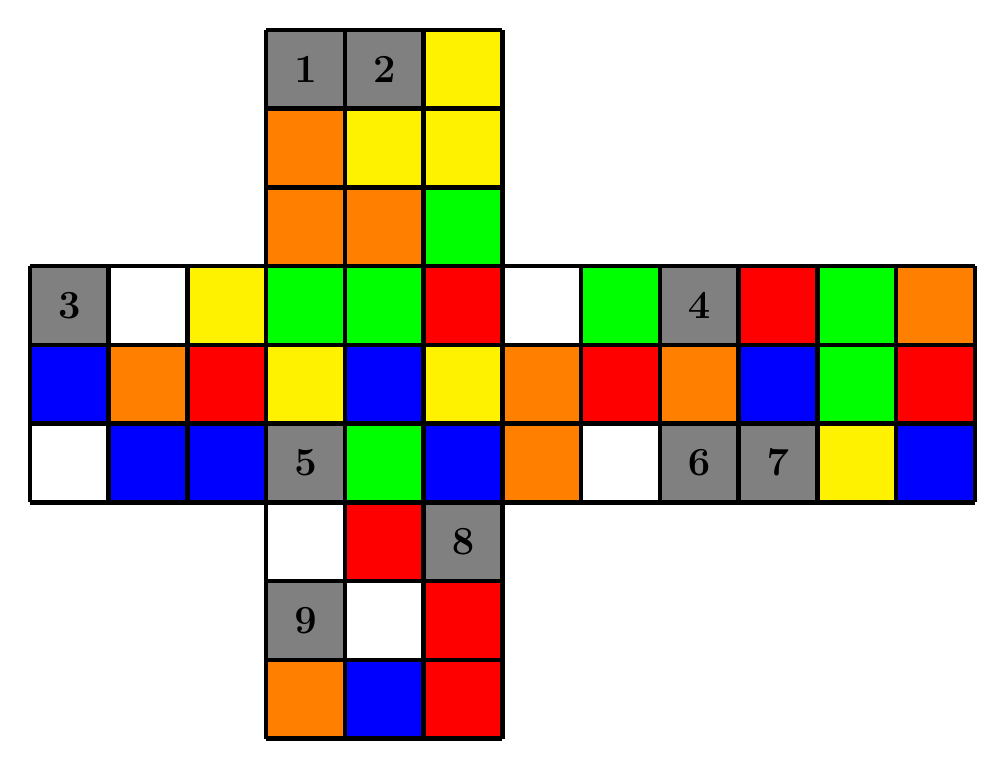
\begin{tikzpicture}[every node/.style={minimum size=1cm-\pgflinewidth, outer sep=0pt}]
\node[fill=gray] at (0.5,5.5) {\Large \textbf 1};
\node[fill=gray] at (1.5,5.5) {\Large \textbf 2};
\node[fill=yellow] at (2.5,5.5) {};
\node[fill=orange] at (0.5,4.5) {};
\node[fill=yellow] at (1.5,4.5) {};
\node[fill=yellow] at (2.5,4.5) {};
\node[fill=orange] at (0.5,3.5) {};
\node[fill=orange] at (1.5,3.5) {};
\node[fill=green] at (2.5,3.5) {};

\node[fill=gray] at (-2.5,2.5) {\Large \textbf 3};
\node[fill=white] at (-1.5,2.5) {};
\node[fill=yellow] at (-0.5,2.5) {};
\node[fill=green] at (0.5,2.5) {};
\node[fill=green] at (1.5,2.5) {};
\node[fill=red] at (2.5,2.5) {};
\node[fill=white] at (3.5,2.5) {};
\node[fill=green] at (4.5,2.5) {};
\node[fill=gray] at (5.5,2.5) {\Large \textbf 4};
\node[fill=red] at (6.5,2.5) {};
\node[fill=green] at (7.5,2.5) {};
\node[fill=orange] at (8.5,2.5) {};

\node[fill=blue] at (-2.5,1.5) {};
\node[fill=orange] at (-1.5,1.5) {};
\node[fill=red] at (-0.5,1.5) {};
\node[fill=yellow] at (0.5,1.5) {};
\node[fill=blue] at (1.5,1.5) {};
\node[fill=yellow] at (2.5,1.5) {};
\node[fill=orange] at (3.5,1.5) {};
\node[fill=red] at (4.5,1.5) {};
\node[fill=orange] at (5.5,1.5) {};
\node[fill=blue] at (6.5,1.5) {};
\node[fill=green] at (7.5,1.5) {};
\node[fill=red] at (8.5,1.5) {};

\node[fill=white] at (-2.5,0.5) {};
\node[fill=blue] at (-1.5,0.5) {};
\node[fill=blue] at (-0.5,0.5) {};
\node[fill=gray] at (0.5,0.5) {\Large \textbf 5};
\node[fill=green] at (1.5,0.5) {};
\node[fill=blue] at (2.5,0.5) {};
\node[fill=orange] at (3.5,0.5) {};
\node[fill=white] at (4.5,0.5) {};
\node[fill=gray] at (5.5,0.5) {\Large \textbf 6};
\node[fill=gray] at (6.5,0.5) {\Large \textbf 7};
\node[fill=yellow] at (7.5,0.5) {};
\node[fill=blue] at (8.5,0.5) {};

\node[fill=white] at (0.5,-0.5) {};
\node[fill=red] at (1.5,-0.5) {};
\node[fill=gray] at (2.5,-0.5) {\Large \textbf 8};
\node[fill=gray] at (0.5,-1.5) {\Large \textbf 9};
\node[fill=white] at (1.5,-1.5) {};
\node[fill=red] at (2.5,-1.5) {};
\node[fill=orange] at (0.5,-2.5) {};
\node[fill=blue] at (1.5,-2.5) {};
\node[fill=red] at (2.5,-2.5) {};

\draw[step=1cm,color=black, ultra thick] (-3,0) grid (9,3);
\draw[step=1cm,color=black, ultra thick] (0,-3) grid (3,0);
\draw[step=1cm,color=black, ultra thick] (0,3) grid (3,6);
\end{tikzpicture}
\vspace{0.1cm}
\\
\noindent\normalsize \newtime  \textbf{Solution 23: U B2 R2 D' B' L2 F R' L' B R' F' D R2 F' L D' R B2 R Uw' }
\vspace{1cm}



{\noindent\Large  \newtime \textbf{No. 24\qquad Difficulty: $\bigstar\bigstar$}}
\vspace{0.2cm}\\
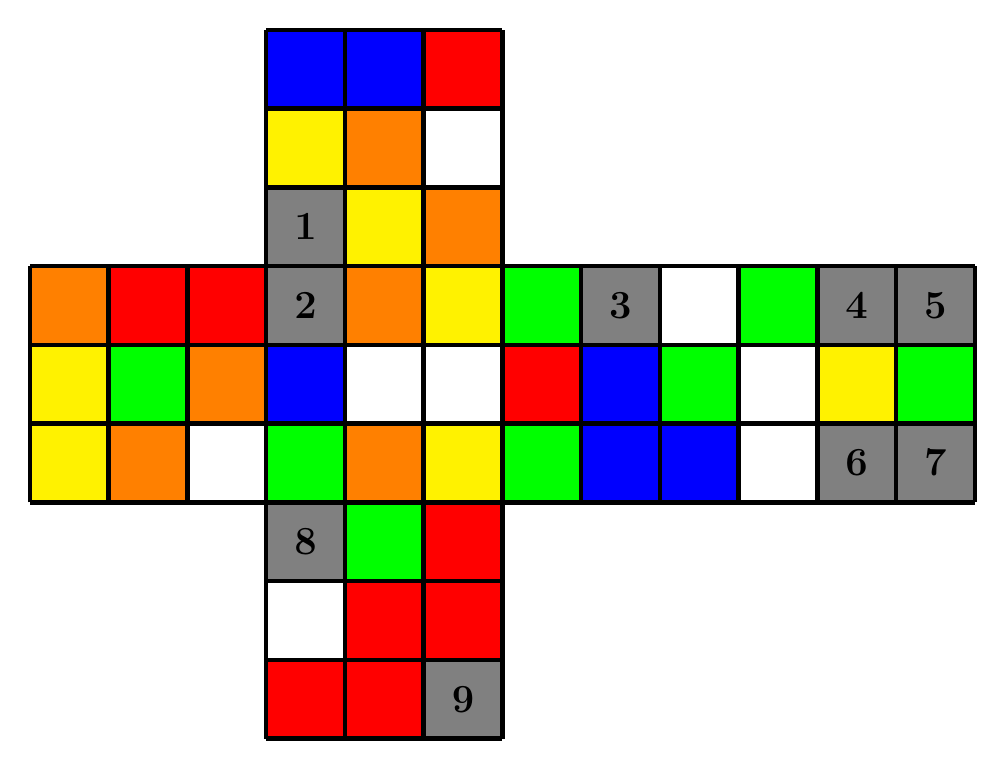
\begin{tikzpicture}[every node/.style={minimum size=1cm-\pgflinewidth, outer sep=0pt}]
\node[fill=blue] at (0.5,5.5) {};
\node[fill=blue] at (1.5,5.5) {};
\node[fill=red] at (2.5,5.5) {};
\node[fill=yellow] at (0.5,4.5) {};
\node[fill=orange] at (1.5,4.5) {};
\node[fill=white] at (2.5,4.5) {};
\node[fill=gray] at (0.5,3.5) {\Large \textbf 1};
\node[fill=yellow] at (1.5,3.5) {};
\node[fill=orange] at (2.5,3.5) {};

\node[fill=orange] at (-2.5,2.5) {};
\node[fill=red] at (-1.5,2.5) {};
\node[fill=red] at (-0.5,2.5) {};
\node[fill=gray] at (0.5,2.5) {\Large \textbf 2};
\node[fill=orange] at (1.5,2.5) {};
\node[fill=yellow] at (2.5,2.5) {};
\node[fill=green] at (3.5,2.5) {};
\node[fill=gray] at (4.5,2.5) {\Large \textbf 3};
\node[fill=white] at (5.5,2.5) {};
\node[fill=green] at (6.5,2.5) {};
\node[fill=gray] at (7.5,2.5) {\Large \textbf 4};
\node[fill=gray] at (8.5,2.5) {\Large \textbf 5};

\node[fill=yellow] at (-2.5,1.5) {};
\node[fill=green] at (-1.5,1.5) {};
\node[fill=orange] at (-0.5,1.5) {};
\node[fill=blue] at (0.5,1.5) {};
\node[fill=white] at (1.5,1.5) {};
\node[fill=white] at (2.5,1.5) {};
\node[fill=red] at (3.5,1.5) {};
\node[fill=blue] at (4.5,1.5) {};
\node[fill=green] at (5.5,1.5) {};
\node[fill=white] at (6.5,1.5) {};
\node[fill=yellow] at (7.5,1.5) {};
\node[fill=green] at (8.5,1.5) {};

\node[fill=yellow] at (-2.5,0.5) {};
\node[fill=orange] at (-1.5,0.5) {};
\node[fill=white] at (-0.5,0.5) {};
\node[fill=green] at (0.5,0.5) {};
\node[fill=orange] at (1.5,0.5) {};
\node[fill=yellow] at (2.5,0.5) {};
\node[fill=green] at (3.5,0.5) {};
\node[fill=blue] at (4.5,0.5) {};
\node[fill=blue] at (5.5,0.5) {};
\node[fill=white] at (6.5,0.5) {};
\node[fill=gray] at (7.5,0.5) {\Large \textbf 6};
\node[fill=gray] at (8.5,0.5) {\Large \textbf 7};

\node[fill=gray] at (0.5,-0.5) {\Large \textbf 8};
\node[fill=green] at (1.5,-0.5) {};
\node[fill=red] at (2.5,-0.5) {};
\node[fill=white] at (0.5,-1.5) {};
\node[fill=red] at (1.5,-1.5) {};
\node[fill=red] at (2.5,-1.5) {};
\node[fill=red] at (0.5,-2.5) {};
\node[fill=red] at (1.5,-2.5) {};
\node[fill=gray] at (2.5,-2.5) {\Large \textbf 9};

\draw[step=1cm,color=black, ultra thick] (-3,0) grid (9,3);
\draw[step=1cm,color=black, ultra thick] (0,-3) grid (3,0);
\draw[step=1cm,color=black, ultra thick] (0,3) grid (3,6);
\end{tikzpicture}
\vspace{0.1cm}
\\
\noindent\normalsize \newtime  \textbf{Solution 24: U B F' R U' R2 L2 U2 F' U2 D2 F2 R2 F' B2 R' F' B' D B Rw' Uw2 }
\vspace{1cm}



{\noindent\Large  \newtime \textbf{No. 25\qquad Difficulty: $\bigstar\bigstar$}}
\vspace{0.2cm}\\
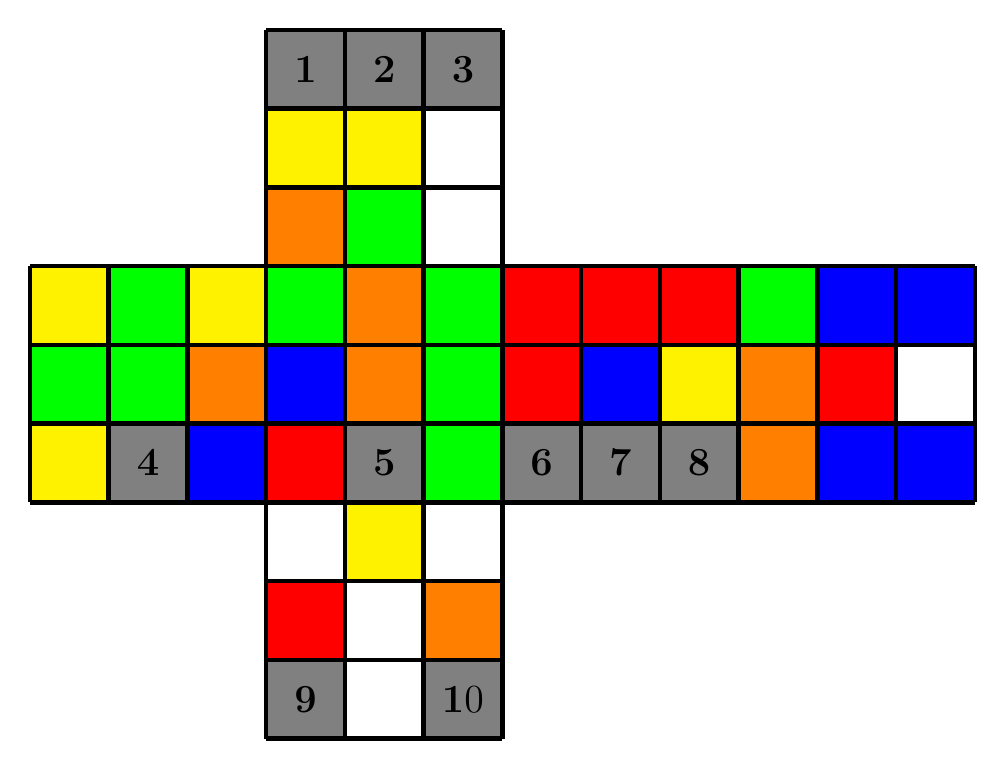
\begin{tikzpicture}[every node/.style={minimum size=1cm-\pgflinewidth, outer sep=0pt}]
\node[fill=gray] at (0.5,5.5) {\Large \textbf 1};
\node[fill=gray] at (1.5,5.5) {\Large \textbf 2};
\node[fill=gray] at (2.5,5.5) {\Large \textbf 3};
\node[fill=yellow] at (0.5,4.5) {};
\node[fill=yellow] at (1.5,4.5) {};
\node[fill=white] at (2.5,4.5) {};
\node[fill=orange] at (0.5,3.5) {};
\node[fill=green] at (1.5,3.5) {};
\node[fill=white] at (2.5,3.5) {};

\node[fill=yellow] at (-2.5,2.5) {};
\node[fill=green] at (-1.5,2.5) {};
\node[fill=yellow] at (-0.5,2.5) {};
\node[fill=green] at (0.5,2.5) {};
\node[fill=orange] at (1.5,2.5) {};
\node[fill=green] at (2.5,2.5) {};
\node[fill=red] at (3.5,2.5) {};
\node[fill=red] at (4.5,2.5) {};
\node[fill=red] at (5.5,2.5) {};
\node[fill=green] at (6.5,2.5) {};
\node[fill=blue] at (7.5,2.5) {};
\node[fill=blue] at (8.5,2.5) {};

\node[fill=green] at (-2.5,1.5) {};
\node[fill=green] at (-1.5,1.5) {};
\node[fill=orange] at (-0.5,1.5) {};
\node[fill=blue] at (0.5,1.5) {};
\node[fill=orange] at (1.5,1.5) {};
\node[fill=green] at (2.5,1.5) {};
\node[fill=red] at (3.5,1.5) {};
\node[fill=blue] at (4.5,1.5) {};
\node[fill=yellow] at (5.5,1.5) {};
\node[fill=orange] at (6.5,1.5) {};
\node[fill=red] at (7.5,1.5) {};
\node[fill=white] at (8.5,1.5) {};

\node[fill=yellow] at (-2.5,0.5) {};
\node[fill=gray] at (-1.5,0.5) {\Large \textbf 4};
\node[fill=blue] at (-0.5,0.5) {};
\node[fill=red] at (0.5,0.5) {};
\node[fill=gray] at (1.5,0.5) {\Large \textbf 5};
\node[fill=green] at (2.5,0.5) {};
\node[fill=gray] at (3.5,0.5) {\Large \textbf 6};
\node[fill=gray] at (4.5,0.5) {\Large \textbf 7};
\node[fill=gray] at (5.5,0.5) {\Large \textbf 8};
\node[fill=orange] at (6.5,0.5) {};
\node[fill=blue] at (7.5,0.5) {};
\node[fill=blue] at (8.5,0.5) {};

\node[fill=white] at (0.5,-0.5) {};
\node[fill=yellow] at (1.5,-0.5) {};
\node[fill=white] at (2.5,-0.5) {};
\node[fill=red] at (0.5,-1.5) {};
\node[fill=white] at (1.5,-1.5) {};
\node[fill=orange] at (2.5,-1.5) {};
\node[fill=gray] at (0.5,-2.5) {\Large \textbf 9};
\node[fill=white] at (1.5,-2.5) {};
\node[fill=gray] at (2.5,-2.5) {\Large \textbf 10};

\draw[step=1cm,color=black, ultra thick] (-3,0) grid (9,3);
\draw[step=1cm,color=black, ultra thick] (0,-3) grid (3,0);
\draw[step=1cm,color=black, ultra thick] (0,3) grid (3,6);
\end{tikzpicture}
\vspace{0.1cm}
\\
\noindent\normalsize \newtime  \textbf{Solution 25: B' R2 B2 D2 U' B' U' B L' R2 F2 D2 R2 D2 U F2 D' R2 U2 R Uw2 }
\vspace{1cm}



{\noindent\Large  \newtime \textbf{No. 26\qquad Difficulty: $\bigstar\bigstar$}}
\vspace{0.2cm}\\
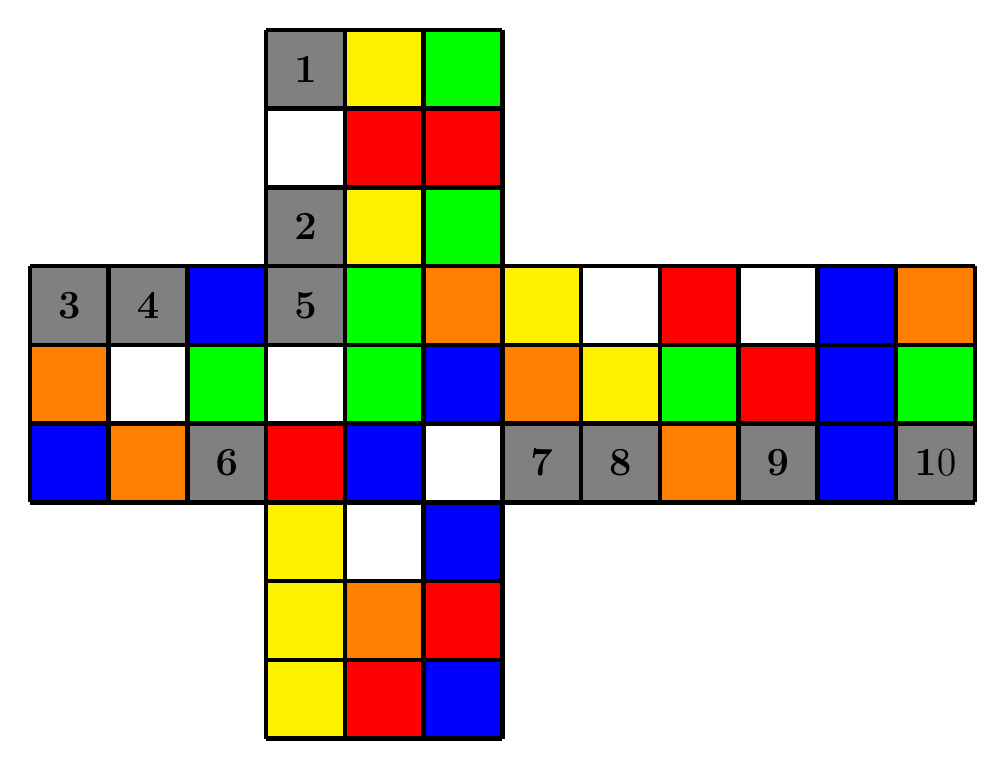
\begin{tikzpicture}[every node/.style={minimum size=1cm-\pgflinewidth, outer sep=0pt}]
\node[fill=gray] at (0.5,5.5) {\Large \textbf 1};
\node[fill=yellow] at (1.5,5.5) {};
\node[fill=green] at (2.5,5.5) {};
\node[fill=white] at (0.5,4.5) {};
\node[fill=red] at (1.5,4.5) {};
\node[fill=red] at (2.5,4.5) {};
\node[fill=gray] at (0.5,3.5) {\Large \textbf 2};
\node[fill=yellow] at (1.5,3.5) {};
\node[fill=green] at (2.5,3.5) {};

\node[fill=gray] at (-2.5,2.5) {\Large \textbf 3};
\node[fill=gray] at (-1.5,2.5) {\Large \textbf 4};
\node[fill=blue] at (-0.5,2.5) {};
\node[fill=gray] at (0.5,2.5) {\Large \textbf 5};
\node[fill=green] at (1.5,2.5) {};
\node[fill=orange] at (2.5,2.5) {};
\node[fill=yellow] at (3.5,2.5) {};
\node[fill=white] at (4.5,2.5) {};
\node[fill=red] at (5.5,2.5) {};
\node[fill=white] at (6.5,2.5) {};
\node[fill=blue] at (7.5,2.5) {};
\node[fill=orange] at (8.5,2.5) {};

\node[fill=orange] at (-2.5,1.5) {};
\node[fill=white] at (-1.5,1.5) {};
\node[fill=green] at (-0.5,1.5) {};
\node[fill=white] at (0.5,1.5) {};
\node[fill=green] at (1.5,1.5) {};
\node[fill=blue] at (2.5,1.5) {};
\node[fill=orange] at (3.5,1.5) {};
\node[fill=yellow] at (4.5,1.5) {};
\node[fill=green] at (5.5,1.5) {};
\node[fill=red] at (6.5,1.5) {};
\node[fill=blue] at (7.5,1.5) {};
\node[fill=green] at (8.5,1.5) {};

\node[fill=blue] at (-2.5,0.5) {};
\node[fill=orange] at (-1.5,0.5) {};
\node[fill=gray] at (-0.5,0.5) {\Large \textbf 6};
\node[fill=red] at (0.5,0.5) {};
\node[fill=blue] at (1.5,0.5) {};
\node[fill=white] at (2.5,0.5) {};
\node[fill=gray] at (3.5,0.5) {\Large \textbf 7};
\node[fill=gray] at (4.5,0.5) {\Large \textbf 8};
\node[fill=orange] at (5.5,0.5) {};
\node[fill=gray] at (6.5,0.5) {\Large \textbf 9};
\node[fill=blue] at (7.5,0.5) {};
\node[fill=gray] at (8.5,0.5) {\Large \textbf 10};

\node[fill=yellow] at (0.5,-0.5) {};
\node[fill=white] at (1.5,-0.5) {};
\node[fill=blue] at (2.5,-0.5) {};
\node[fill=yellow] at (0.5,-1.5) {};
\node[fill=orange] at (1.5,-1.5) {};
\node[fill=red] at (2.5,-1.5) {};
\node[fill=yellow] at (0.5,-2.5) {};
\node[fill=red] at (1.5,-2.5) {};
\node[fill=blue] at (2.5,-2.5) {};

\draw[step=1cm,color=black, ultra thick] (-3,0) grid (9,3);
\draw[step=1cm,color=black, ultra thick] (0,-3) grid (3,0);
\draw[step=1cm,color=black, ultra thick] (0,3) grid (3,6);
\end{tikzpicture}
\vspace{0.1cm}
\\
\noindent\normalsize \newtime  \textbf{Solution 26: B R' F R2 F' B R' B2 L2 U' D2 L U2 L2 R D2 U' F2 L' B Rw Uw }
\vspace{1cm}



{\noindent\Large  \newtime \textbf{No. 27\qquad Difficulty: $\bigstar\bigstar$}}
\vspace{0.2cm}\\
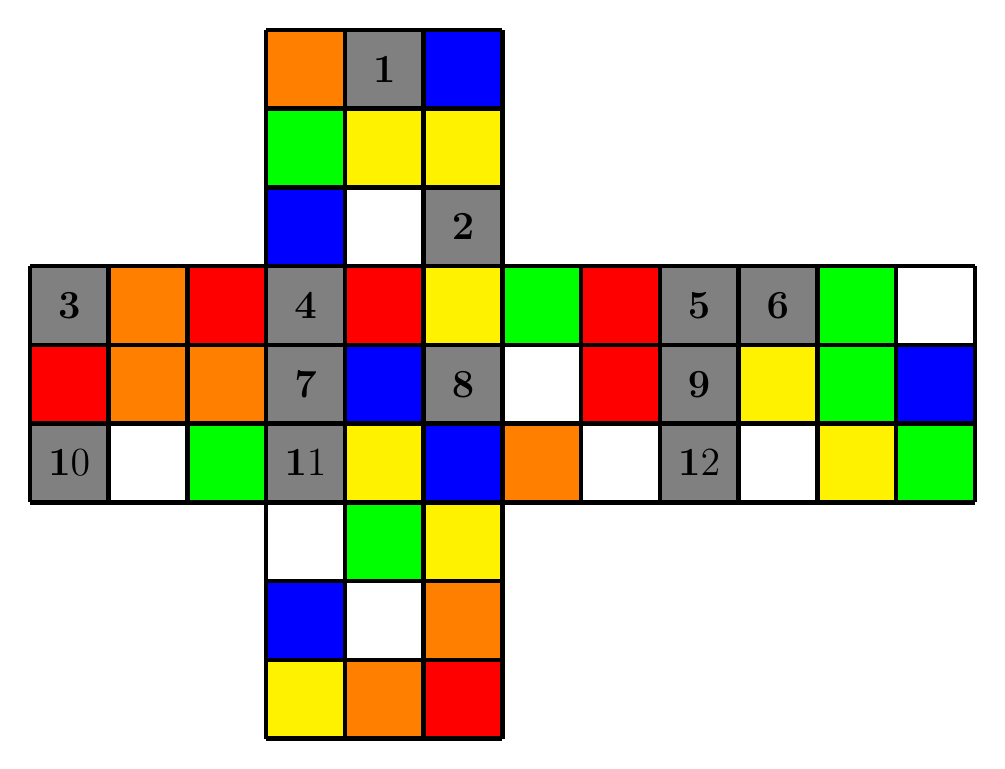
\begin{tikzpicture}[every node/.style={minimum size=1cm-\pgflinewidth, outer sep=0pt}]
\node[fill=orange] at (0.5,5.5) {};
\node[fill=gray] at (1.5,5.5) {\Large \textbf 1};
\node[fill=blue] at (2.5,5.5) {};
\node[fill=green] at (0.5,4.5) {};
\node[fill=yellow] at (1.5,4.5) {};
\node[fill=yellow] at (2.5,4.5) {};
\node[fill=blue] at (0.5,3.5) {};
\node[fill=white] at (1.5,3.5) {};
\node[fill=gray] at (2.5,3.5) {\Large \textbf 2};

\node[fill=gray] at (-2.5,2.5) {\Large \textbf 3};
\node[fill=orange] at (-1.5,2.5) {};
\node[fill=red] at (-0.5,2.5) {};
\node[fill=gray] at (0.5,2.5) {\Large \textbf 4};
\node[fill=red] at (1.5,2.5) {};
\node[fill=yellow] at (2.5,2.5) {};
\node[fill=green] at (3.5,2.5) {};
\node[fill=red] at (4.5,2.5) {};
\node[fill=gray] at (5.5,2.5) {\Large \textbf 5};
\node[fill=gray] at (6.5,2.5) {\Large \textbf 6};
\node[fill=green] at (7.5,2.5) {};
\node[fill=white] at (8.5,2.5) {};

\node[fill=red] at (-2.5,1.5) {};
\node[fill=orange] at (-1.5,1.5) {};
\node[fill=orange] at (-0.5,1.5) {};
\node[fill=gray] at (0.5,1.5) {\Large \textbf 7};
\node[fill=blue] at (1.5,1.5) {};
\node[fill=gray] at (2.5,1.5) {\Large \textbf 8};
\node[fill=white] at (3.5,1.5) {};
\node[fill=red] at (4.5,1.5) {};
\node[fill=gray] at (5.5,1.5) {\Large \textbf 9};
\node[fill=yellow] at (6.5,1.5) {};
\node[fill=green] at (7.5,1.5) {};
\node[fill=blue] at (8.5,1.5) {};

\node[fill=gray] at (-2.5,0.5) {\Large \textbf 10};
\node[fill=white] at (-1.5,0.5) {};
\node[fill=green] at (-0.5,0.5) {};
\node[fill=gray] at (0.5,0.5) {\Large \textbf 11};
\node[fill=yellow] at (1.5,0.5) {};
\node[fill=blue] at (2.5,0.5) {};
\node[fill=orange] at (3.5,0.5) {};
\node[fill=white] at (4.5,0.5) {};
\node[fill=gray] at (5.5,0.5) {\Large \textbf 12};
\node[fill=white] at (6.5,0.5) {};
\node[fill=yellow] at (7.5,0.5) {};
\node[fill=green] at (8.5,0.5) {};

\node[fill=white] at (0.5,-0.5) {};
\node[fill=green] at (1.5,-0.5) {};
\node[fill=yellow] at (2.5,-0.5) {};
\node[fill=blue] at (0.5,-1.5) {};
\node[fill=white] at (1.5,-1.5) {};
\node[fill=orange] at (2.5,-1.5) {};
\node[fill=yellow] at (0.5,-2.5) {};
\node[fill=orange] at (1.5,-2.5) {};
\node[fill=red] at (2.5,-2.5) {};

\draw[step=1cm,color=black, ultra thick] (-3,0) grid (9,3);
\draw[step=1cm,color=black, ultra thick] (0,-3) grid (3,0);
\draw[step=1cm,color=black, ultra thick] (0,3) grid (3,6);
\end{tikzpicture}
\vspace{0.1cm}
\\
\noindent\normalsize \newtime  \textbf{Solution 27: U D L' F' R' F2 R2 L B L D2 U' L' R' U' B D2 L2 R' B' Uw' }
\vspace{1cm}



{\noindent\Large  \newtime \textbf{No. 28\qquad Difficulty: $\bigstar\bigstar$}}
\vspace{0.2cm}\\
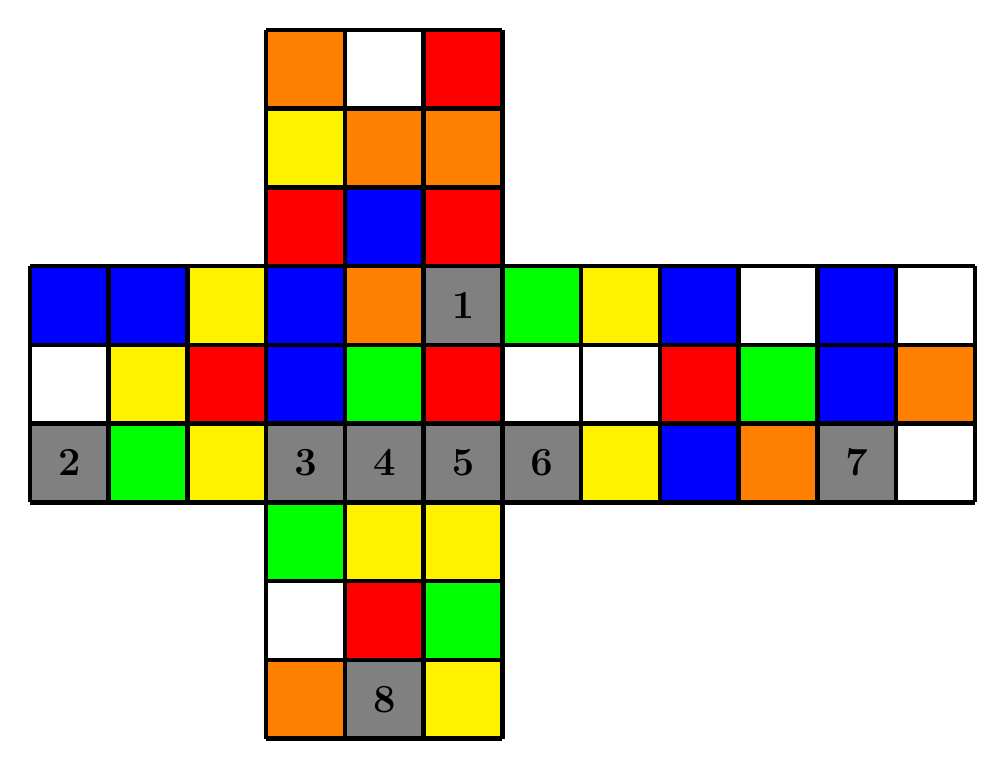
\begin{tikzpicture}[every node/.style={minimum size=1cm-\pgflinewidth, outer sep=0pt}]
\node[fill=orange] at (0.5,5.5) {};
\node[fill=white] at (1.5,5.5) {};
\node[fill=red] at (2.5,5.5) {};
\node[fill=yellow] at (0.5,4.5) {};
\node[fill=orange] at (1.5,4.5) {};
\node[fill=orange] at (2.5,4.5) {};
\node[fill=red] at (0.5,3.5) {};
\node[fill=blue] at (1.5,3.5) {};
\node[fill=red] at (2.5,3.5) {};

\node[fill=blue] at (-2.5,2.5) {};
\node[fill=blue] at (-1.5,2.5) {};
\node[fill=yellow] at (-0.5,2.5) {};
\node[fill=blue] at (0.5,2.5) {};
\node[fill=orange] at (1.5,2.5) {};
\node[fill=gray] at (2.5,2.5) {\Large \textbf 1};
\node[fill=green] at (3.5,2.5) {};
\node[fill=yellow] at (4.5,2.5) {};
\node[fill=blue] at (5.5,2.5) {};
\node[fill=white] at (6.5,2.5) {};
\node[fill=blue] at (7.5,2.5) {};
\node[fill=white] at (8.5,2.5) {};

\node[fill=white] at (-2.5,1.5) {};
\node[fill=yellow] at (-1.5,1.5) {};
\node[fill=red] at (-0.5,1.5) {};
\node[fill=blue] at (0.5,1.5) {};
\node[fill=green] at (1.5,1.5) {};
\node[fill=red] at (2.5,1.5) {};
\node[fill=white] at (3.5,1.5) {};
\node[fill=white] at (4.5,1.5) {};
\node[fill=red] at (5.5,1.5) {};
\node[fill=green] at (6.5,1.5) {};
\node[fill=blue] at (7.5,1.5) {};
\node[fill=orange] at (8.5,1.5) {};

\node[fill=gray] at (-2.5,0.5) {\Large \textbf 2};
\node[fill=green] at (-1.5,0.5) {};
\node[fill=yellow] at (-0.5,0.5) {};
\node[fill=gray] at (0.5,0.5) {\Large \textbf 3};
\node[fill=gray] at (1.5,0.5) {\Large \textbf 4};
\node[fill=gray] at (2.5,0.5) {\Large \textbf 5};
\node[fill=gray] at (3.5,0.5) {\Large \textbf 6};
\node[fill=yellow] at (4.5,0.5) {};
\node[fill=blue] at (5.5,0.5) {};
\node[fill=orange] at (6.5,0.5) {};
\node[fill=gray] at (7.5,0.5) {\Large \textbf 7};
\node[fill=white] at (8.5,0.5) {};

\node[fill=green] at (0.5,-0.5) {};
\node[fill=yellow] at (1.5,-0.5) {};
\node[fill=yellow] at (2.5,-0.5) {};
\node[fill=white] at (0.5,-1.5) {};
\node[fill=red] at (1.5,-1.5) {};
\node[fill=green] at (2.5,-1.5) {};
\node[fill=orange] at (0.5,-2.5) {};
\node[fill=gray] at (1.5,-2.5) {\Large \textbf 8};
\node[fill=yellow] at (2.5,-2.5) {};

\draw[step=1cm,color=black, ultra thick] (-3,0) grid (9,3);
\draw[step=1cm,color=black, ultra thick] (0,-3) grid (3,0);
\draw[step=1cm,color=black, ultra thick] (0,3) grid (3,6);
\end{tikzpicture}
\vspace{0.1cm}
\\
\noindent\normalsize \newtime  \textbf{Solution 28: U2 R' F2 L' U2 R D U L' F2 U' L2 U2 B F U F B' D U' Rw' Uw }
\vspace{1cm}



{\noindent\Large  \newtime \textbf{No. 29\qquad Difficulty: $\bigstar\bigstar$}}
\vspace{0.2cm}\\
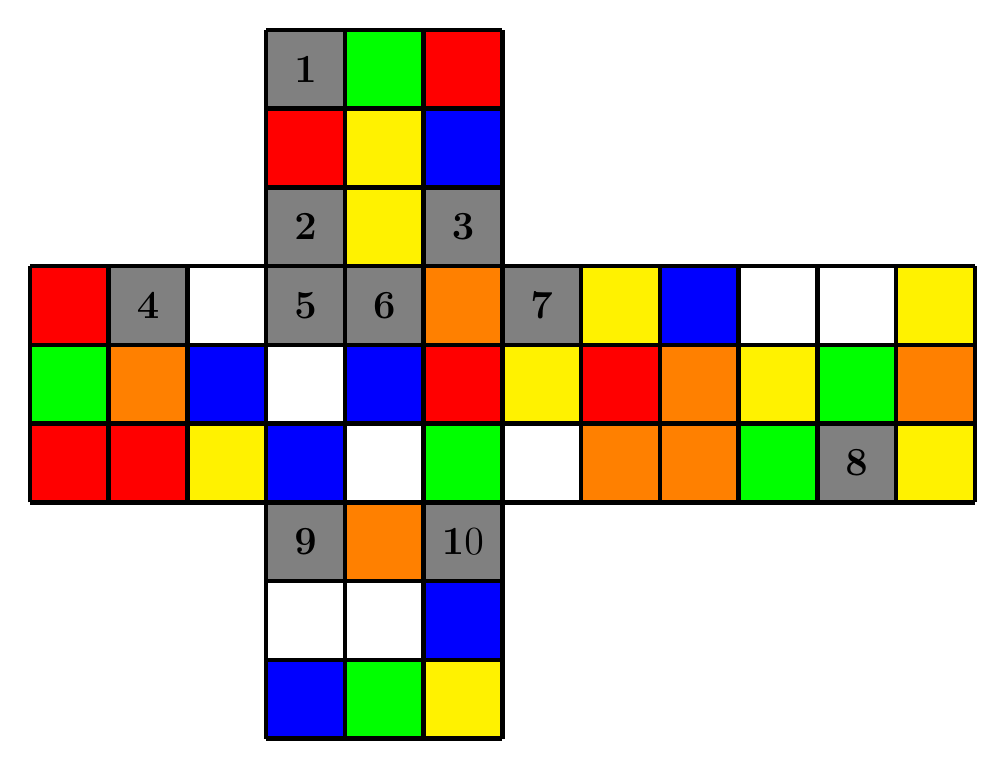
\begin{tikzpicture}[every node/.style={minimum size=1cm-\pgflinewidth, outer sep=0pt}]
\node[fill=gray] at (0.5,5.5) {\Large \textbf 1};
\node[fill=green] at (1.5,5.5) {};
\node[fill=red] at (2.5,5.5) {};
\node[fill=red] at (0.5,4.5) {};
\node[fill=yellow] at (1.5,4.5) {};
\node[fill=blue] at (2.5,4.5) {};
\node[fill=gray] at (0.5,3.5) {\Large \textbf 2};
\node[fill=yellow] at (1.5,3.5) {};
\node[fill=gray] at (2.5,3.5) {\Large \textbf 3};

\node[fill=red] at (-2.5,2.5) {};
\node[fill=gray] at (-1.5,2.5) {\Large \textbf 4};
\node[fill=white] at (-0.5,2.5) {};
\node[fill=gray] at (0.5,2.5) {\Large \textbf 5};
\node[fill=gray] at (1.5,2.5) {\Large \textbf 6};
\node[fill=orange] at (2.5,2.5) {};
\node[fill=gray] at (3.5,2.5) {\Large \textbf 7};
\node[fill=yellow] at (4.5,2.5) {};
\node[fill=blue] at (5.5,2.5) {};
\node[fill=white] at (6.5,2.5) {};
\node[fill=white] at (7.5,2.5) {};
\node[fill=yellow] at (8.5,2.5) {};

\node[fill=green] at (-2.5,1.5) {};
\node[fill=orange] at (-1.5,1.5) {};
\node[fill=blue] at (-0.5,1.5) {};
\node[fill=white] at (0.5,1.5) {};
\node[fill=blue] at (1.5,1.5) {};
\node[fill=red] at (2.5,1.5) {};
\node[fill=yellow] at (3.5,1.5) {};
\node[fill=red] at (4.5,1.5) {};
\node[fill=orange] at (5.5,1.5) {};
\node[fill=yellow] at (6.5,1.5) {};
\node[fill=green] at (7.5,1.5) {};
\node[fill=orange] at (8.5,1.5) {};

\node[fill=red] at (-2.5,0.5) {};
\node[fill=red] at (-1.5,0.5) {};
\node[fill=yellow] at (-0.5,0.5) {};
\node[fill=blue] at (0.5,0.5) {};
\node[fill=white] at (1.5,0.5) {};
\node[fill=green] at (2.5,0.5) {};
\node[fill=white] at (3.5,0.5) {};
\node[fill=orange] at (4.5,0.5) {};
\node[fill=orange] at (5.5,0.5) {};
\node[fill=green] at (6.5,0.5) {};
\node[fill=gray] at (7.5,0.5) {\Large \textbf 8};
\node[fill=yellow] at (8.5,0.5) {};

\node[fill=gray] at (0.5,-0.5) {\Large \textbf 9};
\node[fill=orange] at (1.5,-0.5) {};
\node[fill=gray] at (2.5,-0.5) {\Large \textbf 10};
\node[fill=white] at (0.5,-1.5) {};
\node[fill=white] at (1.5,-1.5) {};
\node[fill=blue] at (2.5,-1.5) {};
\node[fill=blue] at (0.5,-2.5) {};
\node[fill=green] at (1.5,-2.5) {};
\node[fill=yellow] at (2.5,-2.5) {};

\draw[step=1cm,color=black, ultra thick] (-3,0) grid (9,3);
\draw[step=1cm,color=black, ultra thick] (0,-3) grid (3,0);
\draw[step=1cm,color=black, ultra thick] (0,3) grid (3,6);
\end{tikzpicture}
\vspace{0.1cm}
\\
\noindent\normalsize \newtime  \textbf{Solution 29: R L2 U D B' D F' D R2 L D' R U2 L' F R2 U2 R' U' F2 Uw' }
\vspace{1cm}



{\noindent\Large  \newtime \textbf{No. 30\qquad Difficulty: $\bigstar\bigstar$}}
\vspace{0.2cm}\\
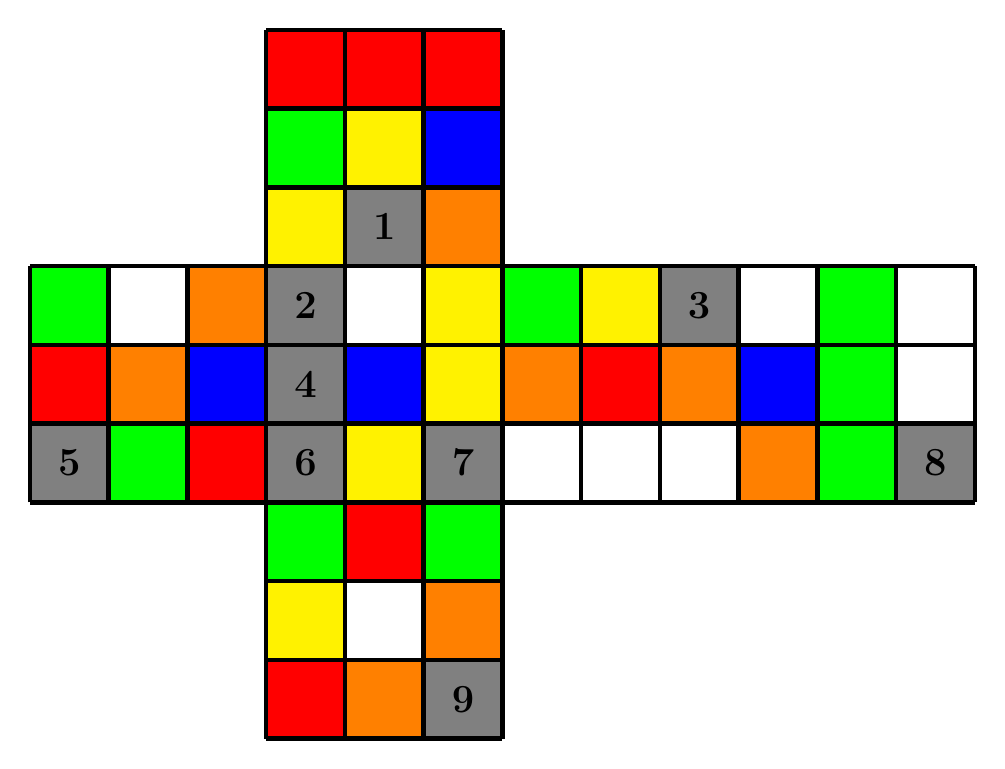
\begin{tikzpicture}[every node/.style={minimum size=1cm-\pgflinewidth, outer sep=0pt}]
\node[fill=red] at (0.5,5.5) {};
\node[fill=red] at (1.5,5.5) {};
\node[fill=red] at (2.5,5.5) {};
\node[fill=green] at (0.5,4.5) {};
\node[fill=yellow] at (1.5,4.5) {};
\node[fill=blue] at (2.5,4.5) {};
\node[fill=yellow] at (0.5,3.5) {};
\node[fill=gray] at (1.5,3.5) {\Large \textbf 1};
\node[fill=orange] at (2.5,3.5) {};

\node[fill=green] at (-2.5,2.5) {};
\node[fill=white] at (-1.5,2.5) {};
\node[fill=orange] at (-0.5,2.5) {};
\node[fill=gray] at (0.5,2.5) {\Large \textbf 2};
\node[fill=white] at (1.5,2.5) {};
\node[fill=yellow] at (2.5,2.5) {};
\node[fill=green] at (3.5,2.5) {};
\node[fill=yellow] at (4.5,2.5) {};
\node[fill=gray] at (5.5,2.5) {\Large \textbf 3};
\node[fill=white] at (6.5,2.5) {};
\node[fill=green] at (7.5,2.5) {};
\node[fill=white] at (8.5,2.5) {};

\node[fill=red] at (-2.5,1.5) {};
\node[fill=orange] at (-1.5,1.5) {};
\node[fill=blue] at (-0.5,1.5) {};
\node[fill=gray] at (0.5,1.5) {\Large \textbf 4};
\node[fill=blue] at (1.5,1.5) {};
\node[fill=yellow] at (2.5,1.5) {};
\node[fill=orange] at (3.5,1.5) {};
\node[fill=red] at (4.5,1.5) {};
\node[fill=orange] at (5.5,1.5) {};
\node[fill=blue] at (6.5,1.5) {};
\node[fill=green] at (7.5,1.5) {};
\node[fill=white] at (8.5,1.5) {};

\node[fill=gray] at (-2.5,0.5) {\Large \textbf 5};
\node[fill=green] at (-1.5,0.5) {};
\node[fill=red] at (-0.5,0.5) {};
\node[fill=gray] at (0.5,0.5) {\Large \textbf 6};
\node[fill=yellow] at (1.5,0.5) {};
\node[fill=gray] at (2.5,0.5) {\Large \textbf 7};
\node[fill=white] at (3.5,0.5) {};
\node[fill=white] at (4.5,0.5) {};
\node[fill=white] at (5.5,0.5) {};
\node[fill=orange] at (6.5,0.5) {};
\node[fill=green] at (7.5,0.5) {};
\node[fill=gray] at (8.5,0.5) {\Large \textbf 8};

\node[fill=green] at (0.5,-0.5) {};
\node[fill=red] at (1.5,-0.5) {};
\node[fill=green] at (2.5,-0.5) {};
\node[fill=yellow] at (0.5,-1.5) {};
\node[fill=white] at (1.5,-1.5) {};
\node[fill=orange] at (2.5,-1.5) {};
\node[fill=red] at (0.5,-2.5) {};
\node[fill=orange] at (1.5,-2.5) {};
\node[fill=gray] at (2.5,-2.5) {\Large \textbf 9};

\draw[step=1cm,color=black, ultra thick] (-3,0) grid (9,3);
\draw[step=1cm,color=black, ultra thick] (0,-3) grid (3,0);
\draw[step=1cm,color=black, ultra thick] (0,3) grid (3,6);
\end{tikzpicture}
\vspace{0.1cm}
\\
\noindent\normalsize \newtime  \textbf{Solution 30: R2 D2 B D' B' F' D B2 D' B' U2 B' D' R B L F D U2 R Uw' }
\vspace{1cm}



{\noindent\Large  \newtime \textbf{No. 31\qquad Difficulty: $\bigstar\bigstar$}}
\vspace{0.2cm}\\
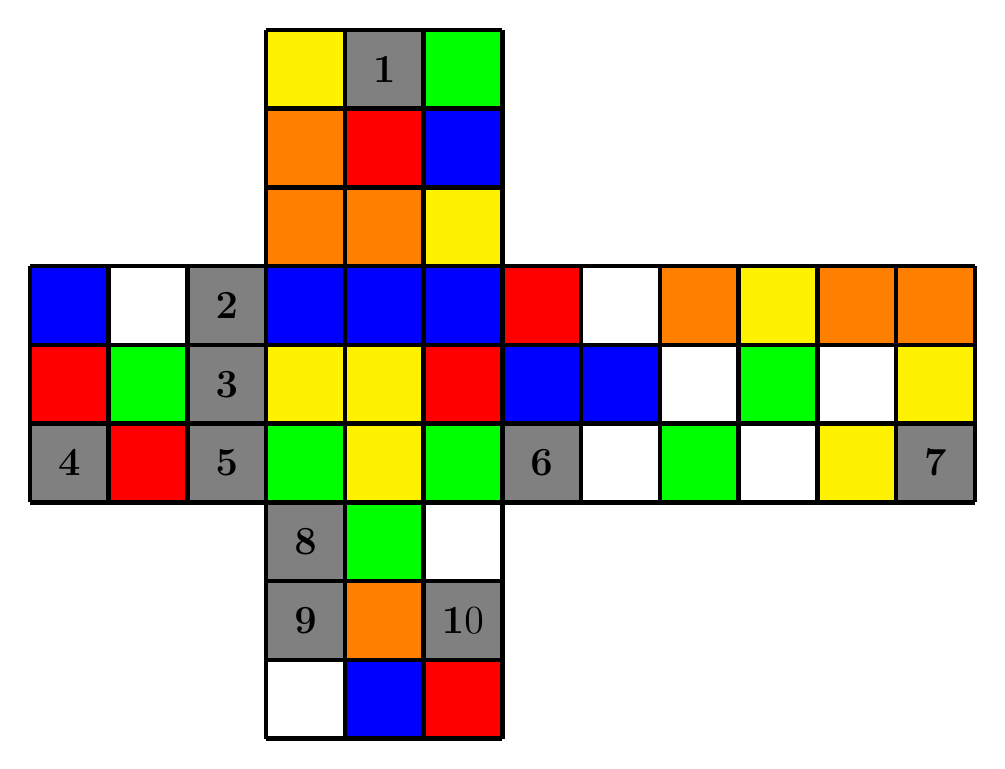
\begin{tikzpicture}[every node/.style={minimum size=1cm-\pgflinewidth, outer sep=0pt}]
\node[fill=yellow] at (0.5,5.5) {};
\node[fill=gray] at (1.5,5.5) {\Large \textbf 1};
\node[fill=green] at (2.5,5.5) {};
\node[fill=orange] at (0.5,4.5) {};
\node[fill=red] at (1.5,4.5) {};
\node[fill=blue] at (2.5,4.5) {};
\node[fill=orange] at (0.5,3.5) {};
\node[fill=orange] at (1.5,3.5) {};
\node[fill=yellow] at (2.5,3.5) {};

\node[fill=blue] at (-2.5,2.5) {};
\node[fill=white] at (-1.5,2.5) {};
\node[fill=gray] at (-0.5,2.5) {\Large \textbf 2};
\node[fill=blue] at (0.5,2.5) {};
\node[fill=blue] at (1.5,2.5) {};
\node[fill=blue] at (2.5,2.5) {};
\node[fill=red] at (3.5,2.5) {};
\node[fill=white] at (4.5,2.5) {};
\node[fill=orange] at (5.5,2.5) {};
\node[fill=yellow] at (6.5,2.5) {};
\node[fill=orange] at (7.5,2.5) {};
\node[fill=orange] at (8.5,2.5) {};

\node[fill=red] at (-2.5,1.5) {};
\node[fill=green] at (-1.5,1.5) {};
\node[fill=gray] at (-0.5,1.5) {\Large \textbf 3};
\node[fill=yellow] at (0.5,1.5) {};
\node[fill=yellow] at (1.5,1.5) {};
\node[fill=red] at (2.5,1.5) {};
\node[fill=blue] at (3.5,1.5) {};
\node[fill=blue] at (4.5,1.5) {};
\node[fill=white] at (5.5,1.5) {};
\node[fill=green] at (6.5,1.5) {};
\node[fill=white] at (7.5,1.5) {};
\node[fill=yellow] at (8.5,1.5) {};

\node[fill=gray] at (-2.5,0.5) {\Large \textbf 4};
\node[fill=red] at (-1.5,0.5) {};
\node[fill=gray] at (-0.5,0.5) {\Large \textbf 5};
\node[fill=green] at (0.5,0.5) {};
\node[fill=yellow] at (1.5,0.5) {};
\node[fill=green] at (2.5,0.5) {};
\node[fill=gray] at (3.5,0.5) {\Large \textbf 6};
\node[fill=white] at (4.5,0.5) {};
\node[fill=green] at (5.5,0.5) {};
\node[fill=white] at (6.5,0.5) {};
\node[fill=yellow] at (7.5,0.5) {};
\node[fill=gray] at (8.5,0.5) {\Large \textbf 7};

\node[fill=gray] at (0.5,-0.5) {\Large \textbf 8};
\node[fill=green] at (1.5,-0.5) {};
\node[fill=white] at (2.5,-0.5) {};
\node[fill=gray] at (0.5,-1.5) {\Large \textbf 9};
\node[fill=orange] at (1.5,-1.5) {};
\node[fill=gray] at (2.5,-1.5) {\Large \textbf 10};
\node[fill=white] at (0.5,-2.5) {};
\node[fill=blue] at (1.5,-2.5) {};
\node[fill=red] at (2.5,-2.5) {};

\draw[step=1cm,color=black, ultra thick] (-3,0) grid (9,3);
\draw[step=1cm,color=black, ultra thick] (0,-3) grid (3,0);
\draw[step=1cm,color=black, ultra thick] (0,3) grid (3,6);
\end{tikzpicture}
\vspace{0.1cm}
\\
\noindent\normalsize \newtime  \textbf{Solution 31: F' B2 L F2 D F B' D R' F U' R' U F' R2 F2 R L2 D U' Rw Uw2 }
\vspace{1cm}



{\noindent\Large  \newtime \textbf{No. 32\qquad Difficulty: $\bigstar\bigstar$}}
\vspace{0.2cm}\\
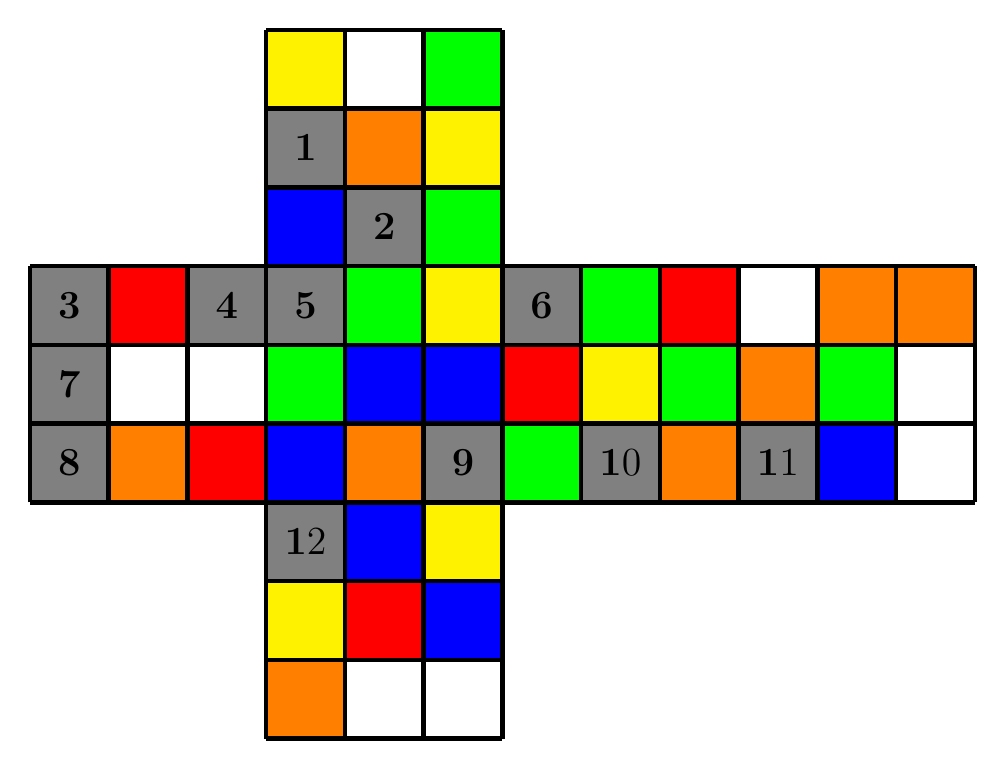
\begin{tikzpicture}[every node/.style={minimum size=1cm-\pgflinewidth, outer sep=0pt}]
\node[fill=yellow] at (0.5,5.5) {};
\node[fill=white] at (1.5,5.5) {};
\node[fill=green] at (2.5,5.5) {};
\node[fill=gray] at (0.5,4.5) {\Large \textbf 1};
\node[fill=orange] at (1.5,4.5) {};
\node[fill=yellow] at (2.5,4.5) {};
\node[fill=blue] at (0.5,3.5) {};
\node[fill=gray] at (1.5,3.5) {\Large \textbf 2};
\node[fill=green] at (2.5,3.5) {};

\node[fill=gray] at (-2.5,2.5) {\Large \textbf 3};
\node[fill=red] at (-1.5,2.5) {};
\node[fill=gray] at (-0.5,2.5) {\Large \textbf 4};
\node[fill=gray] at (0.5,2.5) {\Large \textbf 5};
\node[fill=green] at (1.5,2.5) {};
\node[fill=yellow] at (2.5,2.5) {};
\node[fill=gray] at (3.5,2.5) {\Large \textbf 6};
\node[fill=green] at (4.5,2.5) {};
\node[fill=red] at (5.5,2.5) {};
\node[fill=white] at (6.5,2.5) {};
\node[fill=orange] at (7.5,2.5) {};
\node[fill=orange] at (8.5,2.5) {};

\node[fill=gray] at (-2.5,1.5) {\Large \textbf 7};
\node[fill=white] at (-1.5,1.5) {};
\node[fill=white] at (-0.5,1.5) {};
\node[fill=green] at (0.5,1.5) {};
\node[fill=blue] at (1.5,1.5) {};
\node[fill=blue] at (2.5,1.5) {};
\node[fill=red] at (3.5,1.5) {};
\node[fill=yellow] at (4.5,1.5) {};
\node[fill=green] at (5.5,1.5) {};
\node[fill=orange] at (6.5,1.5) {};
\node[fill=green] at (7.5,1.5) {};
\node[fill=white] at (8.5,1.5) {};

\node[fill=gray] at (-2.5,0.5) {\Large \textbf 8};
\node[fill=orange] at (-1.5,0.5) {};
\node[fill=red] at (-0.5,0.5) {};
\node[fill=blue] at (0.5,0.5) {};
\node[fill=orange] at (1.5,0.5) {};
\node[fill=gray] at (2.5,0.5) {\Large \textbf 9};
\node[fill=green] at (3.5,0.5) {};
\node[fill=gray] at (4.5,0.5) {\Large \textbf 10};
\node[fill=orange] at (5.5,0.5) {};
\node[fill=gray] at (6.5,0.5) {\Large \textbf 11};
\node[fill=blue] at (7.5,0.5) {};
\node[fill=white] at (8.5,0.5) {};

\node[fill=gray] at (0.5,-0.5) {\Large \textbf 12};
\node[fill=blue] at (1.5,-0.5) {};
\node[fill=yellow] at (2.5,-0.5) {};
\node[fill=yellow] at (0.5,-1.5) {};
\node[fill=red] at (1.5,-1.5) {};
\node[fill=blue] at (2.5,-1.5) {};
\node[fill=orange] at (0.5,-2.5) {};
\node[fill=white] at (1.5,-2.5) {};
\node[fill=white] at (2.5,-2.5) {};

\draw[step=1cm,color=black, ultra thick] (-3,0) grid (9,3);
\draw[step=1cm,color=black, ultra thick] (0,-3) grid (3,0);
\draw[step=1cm,color=black, ultra thick] (0,3) grid (3,6);
\end{tikzpicture}
\vspace{0.1cm}
\\
\noindent\normalsize \newtime  \textbf{Solution 32: R2 F2 R2 U' L D' F' B' U2 F2 U' L' F R' F' B' U L2 B U2 Rw' Uw' }
\vspace{1cm}



{\noindent\Large  \newtime \textbf{No. 33\qquad Difficulty: $\bigstar\bigstar$}}
\vspace{0.2cm}\\
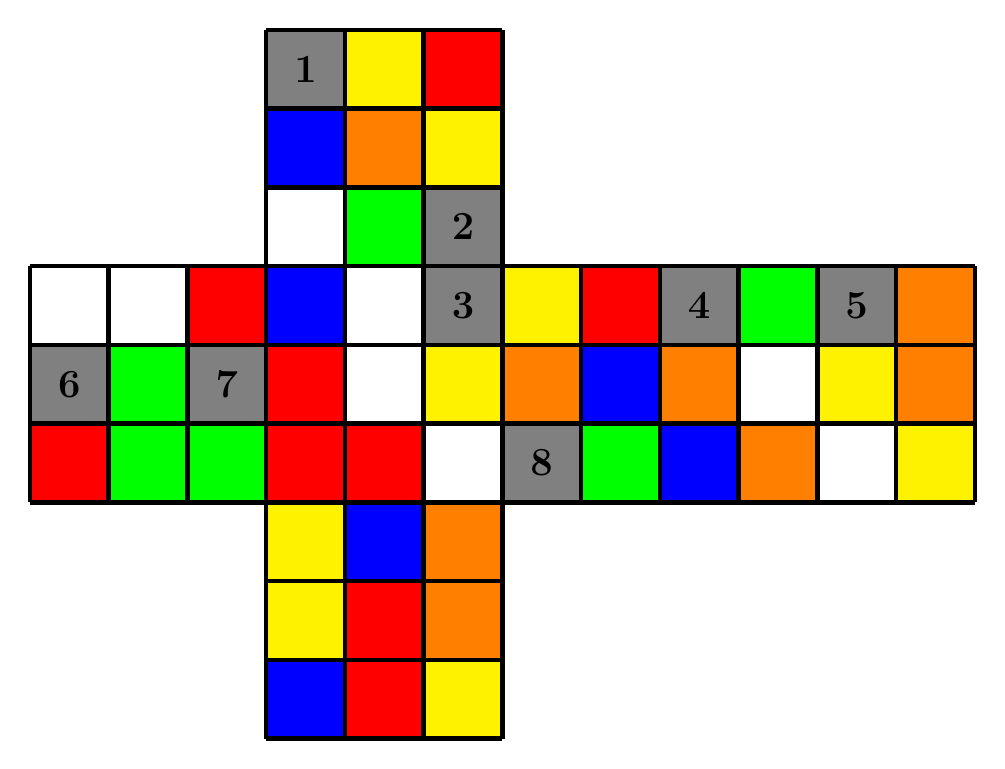
\begin{tikzpicture}[every node/.style={minimum size=1cm-\pgflinewidth, outer sep=0pt}]
\node[fill=gray] at (0.5,5.5) {\Large \textbf 1};
\node[fill=yellow] at (1.5,5.5) {};
\node[fill=red] at (2.5,5.5) {};
\node[fill=blue] at (0.5,4.5) {};
\node[fill=orange] at (1.5,4.5) {};
\node[fill=yellow] at (2.5,4.5) {};
\node[fill=white] at (0.5,3.5) {};
\node[fill=green] at (1.5,3.5) {};
\node[fill=gray] at (2.5,3.5) {\Large \textbf 2};

\node[fill=white] at (-2.5,2.5) {};
\node[fill=white] at (-1.5,2.5) {};
\node[fill=red] at (-0.5,2.5) {};
\node[fill=blue] at (0.5,2.5) {};
\node[fill=white] at (1.5,2.5) {};
\node[fill=gray] at (2.5,2.5) {\Large \textbf 3};
\node[fill=yellow] at (3.5,2.5) {};
\node[fill=red] at (4.5,2.5) {};
\node[fill=gray] at (5.5,2.5) {\Large \textbf 4};
\node[fill=green] at (6.5,2.5) {};
\node[fill=gray] at (7.5,2.5) {\Large \textbf 5};
\node[fill=orange] at (8.5,2.5) {};

\node[fill=gray] at (-2.5,1.5) {\Large \textbf 6};
\node[fill=green] at (-1.5,1.5) {};
\node[fill=gray] at (-0.5,1.5) {\Large \textbf 7};
\node[fill=red] at (0.5,1.5) {};
\node[fill=white] at (1.5,1.5) {};
\node[fill=yellow] at (2.5,1.5) {};
\node[fill=orange] at (3.5,1.5) {};
\node[fill=blue] at (4.5,1.5) {};
\node[fill=orange] at (5.5,1.5) {};
\node[fill=white] at (6.5,1.5) {};
\node[fill=yellow] at (7.5,1.5) {};
\node[fill=orange] at (8.5,1.5) {};

\node[fill=red] at (-2.5,0.5) {};
\node[fill=green] at (-1.5,0.5) {};
\node[fill=green] at (-0.5,0.5) {};
\node[fill=red] at (0.5,0.5) {};
\node[fill=red] at (1.5,0.5) {};
\node[fill=white] at (2.5,0.5) {};
\node[fill=gray] at (3.5,0.5) {\Large \textbf 8};
\node[fill=green] at (4.5,0.5) {};
\node[fill=blue] at (5.5,0.5) {};
\node[fill=orange] at (6.5,0.5) {};
\node[fill=white] at (7.5,0.5) {};
\node[fill=yellow] at (8.5,0.5) {};

\node[fill=yellow] at (0.5,-0.5) {};
\node[fill=blue] at (1.5,-0.5) {};
\node[fill=orange] at (2.5,-0.5) {};
\node[fill=yellow] at (0.5,-1.5) {};
\node[fill=red] at (1.5,-1.5) {};
\node[fill=orange] at (2.5,-1.5) {};
\node[fill=blue] at (0.5,-2.5) {};
\node[fill=red] at (1.5,-2.5) {};
\node[fill=yellow] at (2.5,-2.5) {};

\draw[step=1cm,color=black, ultra thick] (-3,0) grid (9,3);
\draw[step=1cm,color=black, ultra thick] (0,-3) grid (3,0);
\draw[step=1cm,color=black, ultra thick] (0,3) grid (3,6);
\end{tikzpicture}
\vspace{0.1cm}
\\
\noindent\normalsize \newtime  \textbf{Solution 33: F' L D' B2 F R D L2 B' F2 D' L2 F2 B2 R2 F2 U F' L F Rw' Uw2 }
\vspace{1cm}



{\noindent\Large  \newtime \textbf{No. 34\qquad Difficulty: $\bigstar\bigstar$}}
\vspace{0.2cm}\\
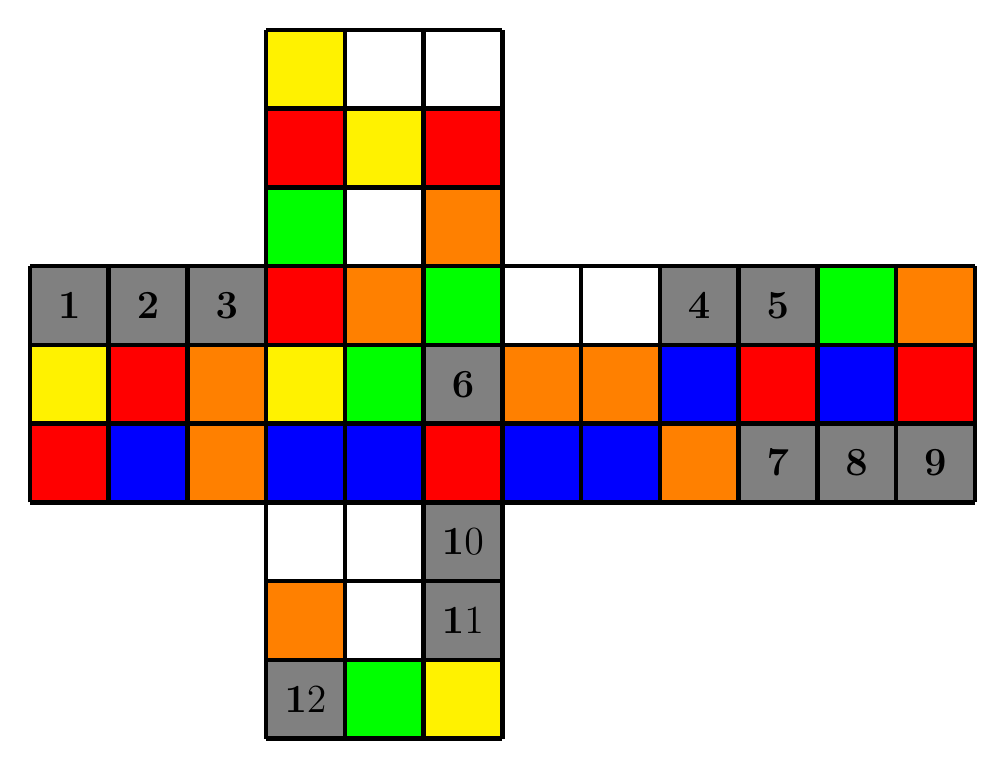
\begin{tikzpicture}[every node/.style={minimum size=1cm-\pgflinewidth, outer sep=0pt}]
\node[fill=yellow] at (0.5,5.5) {};
\node[fill=white] at (1.5,5.5) {};
\node[fill=white] at (2.5,5.5) {};
\node[fill=red] at (0.5,4.5) {};
\node[fill=yellow] at (1.5,4.5) {};
\node[fill=red] at (2.5,4.5) {};
\node[fill=green] at (0.5,3.5) {};
\node[fill=white] at (1.5,3.5) {};
\node[fill=orange] at (2.5,3.5) {};

\node[fill=gray] at (-2.5,2.5) {\Large \textbf 1};
\node[fill=gray] at (-1.5,2.5) {\Large \textbf 2};
\node[fill=gray] at (-0.5,2.5) {\Large \textbf 3};
\node[fill=red] at (0.5,2.5) {};
\node[fill=orange] at (1.5,2.5) {};
\node[fill=green] at (2.5,2.5) {};
\node[fill=white] at (3.5,2.5) {};
\node[fill=white] at (4.5,2.5) {};
\node[fill=gray] at (5.5,2.5) {\Large \textbf 4};
\node[fill=gray] at (6.5,2.5) {\Large \textbf 5};
\node[fill=green] at (7.5,2.5) {};
\node[fill=orange] at (8.5,2.5) {};

\node[fill=yellow] at (-2.5,1.5) {};
\node[fill=red] at (-1.5,1.5) {};
\node[fill=orange] at (-0.5,1.5) {};
\node[fill=yellow] at (0.5,1.5) {};
\node[fill=green] at (1.5,1.5) {};
\node[fill=gray] at (2.5,1.5) {\Large \textbf 6};
\node[fill=orange] at (3.5,1.5) {};
\node[fill=orange] at (4.5,1.5) {};
\node[fill=blue] at (5.5,1.5) {};
\node[fill=red] at (6.5,1.5) {};
\node[fill=blue] at (7.5,1.5) {};
\node[fill=red] at (8.5,1.5) {};

\node[fill=red] at (-2.5,0.5) {};
\node[fill=blue] at (-1.5,0.5) {};
\node[fill=orange] at (-0.5,0.5) {};
\node[fill=blue] at (0.5,0.5) {};
\node[fill=blue] at (1.5,0.5) {};
\node[fill=red] at (2.5,0.5) {};
\node[fill=blue] at (3.5,0.5) {};
\node[fill=blue] at (4.5,0.5) {};
\node[fill=orange] at (5.5,0.5) {};
\node[fill=gray] at (6.5,0.5) {\Large \textbf 7};
\node[fill=gray] at (7.5,0.5) {\Large \textbf 8};
\node[fill=gray] at (8.5,0.5) {\Large \textbf 9};

\node[fill=white] at (0.5,-0.5) {};
\node[fill=white] at (1.5,-0.5) {};
\node[fill=gray] at (2.5,-0.5) {\Large \textbf 10};
\node[fill=orange] at (0.5,-1.5) {};
\node[fill=white] at (1.5,-1.5) {};
\node[fill=gray] at (2.5,-1.5) {\Large \textbf 11};
\node[fill=gray] at (0.5,-2.5) {\Large \textbf 12};
\node[fill=green] at (1.5,-2.5) {};
\node[fill=yellow] at (2.5,-2.5) {};

\draw[step=1cm,color=black, ultra thick] (-3,0) grid (9,3);
\draw[step=1cm,color=black, ultra thick] (0,-3) grid (3,0);
\draw[step=1cm,color=black, ultra thick] (0,3) grid (3,6);
\end{tikzpicture}
\vspace{0.1cm}
\\
\noindent\normalsize \newtime  \textbf{Solution 34: F2 R L' B2 U' R D F D F' L' R2 D2 F2 B2 U' L2 R' F2 B' Uw }
\vspace{1cm}



{\noindent\Large  \newtime \textbf{No. 35\qquad Difficulty: $\bigstar\bigstar$}}
\vspace{0.2cm}\\
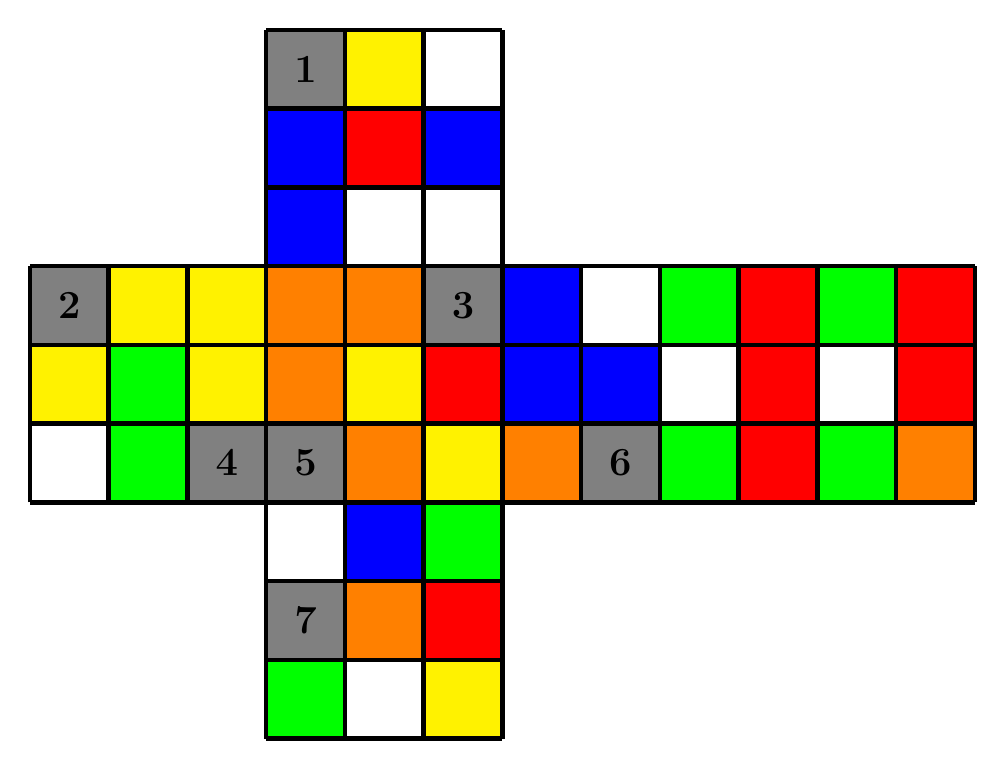
\begin{tikzpicture}[every node/.style={minimum size=1cm-\pgflinewidth, outer sep=0pt}]
\node[fill=gray] at (0.5,5.5) {\Large \textbf 1};
\node[fill=yellow] at (1.5,5.5) {};
\node[fill=white] at (2.5,5.5) {};
\node[fill=blue] at (0.5,4.5) {};
\node[fill=red] at (1.5,4.5) {};
\node[fill=blue] at (2.5,4.5) {};
\node[fill=blue] at (0.5,3.5) {};
\node[fill=white] at (1.5,3.5) {};
\node[fill=white] at (2.5,3.5) {};

\node[fill=gray] at (-2.5,2.5) {\Large \textbf 2};
\node[fill=yellow] at (-1.5,2.5) {};
\node[fill=yellow] at (-0.5,2.5) {};
\node[fill=orange] at (0.5,2.5) {};
\node[fill=orange] at (1.5,2.5) {};
\node[fill=gray] at (2.5,2.5) {\Large \textbf 3};
\node[fill=blue] at (3.5,2.5) {};
\node[fill=white] at (4.5,2.5) {};
\node[fill=green] at (5.5,2.5) {};
\node[fill=red] at (6.5,2.5) {};
\node[fill=green] at (7.5,2.5) {};
\node[fill=red] at (8.5,2.5) {};

\node[fill=yellow] at (-2.5,1.5) {};
\node[fill=green] at (-1.5,1.5) {};
\node[fill=yellow] at (-0.5,1.5) {};
\node[fill=orange] at (0.5,1.5) {};
\node[fill=yellow] at (1.5,1.5) {};
\node[fill=red] at (2.5,1.5) {};
\node[fill=blue] at (3.5,1.5) {};
\node[fill=blue] at (4.5,1.5) {};
\node[fill=white] at (5.5,1.5) {};
\node[fill=red] at (6.5,1.5) {};
\node[fill=white] at (7.5,1.5) {};
\node[fill=red] at (8.5,1.5) {};

\node[fill=white] at (-2.5,0.5) {};
\node[fill=green] at (-1.5,0.5) {};
\node[fill=gray] at (-0.5,0.5) {\Large \textbf 4};
\node[fill=gray] at (0.5,0.5) {\Large \textbf 5};
\node[fill=orange] at (1.5,0.5) {};
\node[fill=yellow] at (2.5,0.5) {};
\node[fill=orange] at (3.5,0.5) {};
\node[fill=gray] at (4.5,0.5) {\Large \textbf 6};
\node[fill=green] at (5.5,0.5) {};
\node[fill=red] at (6.5,0.5) {};
\node[fill=green] at (7.5,0.5) {};
\node[fill=orange] at (8.5,0.5) {};

\node[fill=white] at (0.5,-0.5) {};
\node[fill=blue] at (1.5,-0.5) {};
\node[fill=green] at (2.5,-0.5) {};
\node[fill=gray] at (0.5,-1.5) {\Large \textbf 7};
\node[fill=orange] at (1.5,-1.5) {};
\node[fill=red] at (2.5,-1.5) {};
\node[fill=green] at (0.5,-2.5) {};
\node[fill=white] at (1.5,-2.5) {};
\node[fill=yellow] at (2.5,-2.5) {};

\draw[step=1cm,color=black, ultra thick] (-3,0) grid (9,3);
\draw[step=1cm,color=black, ultra thick] (0,-3) grid (3,0);
\draw[step=1cm,color=black, ultra thick] (0,3) grid (3,6);
\end{tikzpicture}
\vspace{0.1cm}
\\
\noindent\normalsize \newtime  \textbf{Solution 35: U F R2 D2 F L B D' L B' R2 L U2 R2 F' R U2 B F' D' Rw Uw2 }
\vspace{1cm}



{\noindent\Large  \newtime \textbf{No. 36\qquad Difficulty: $\bigstar\bigstar$}}
\vspace{0.2cm}\\
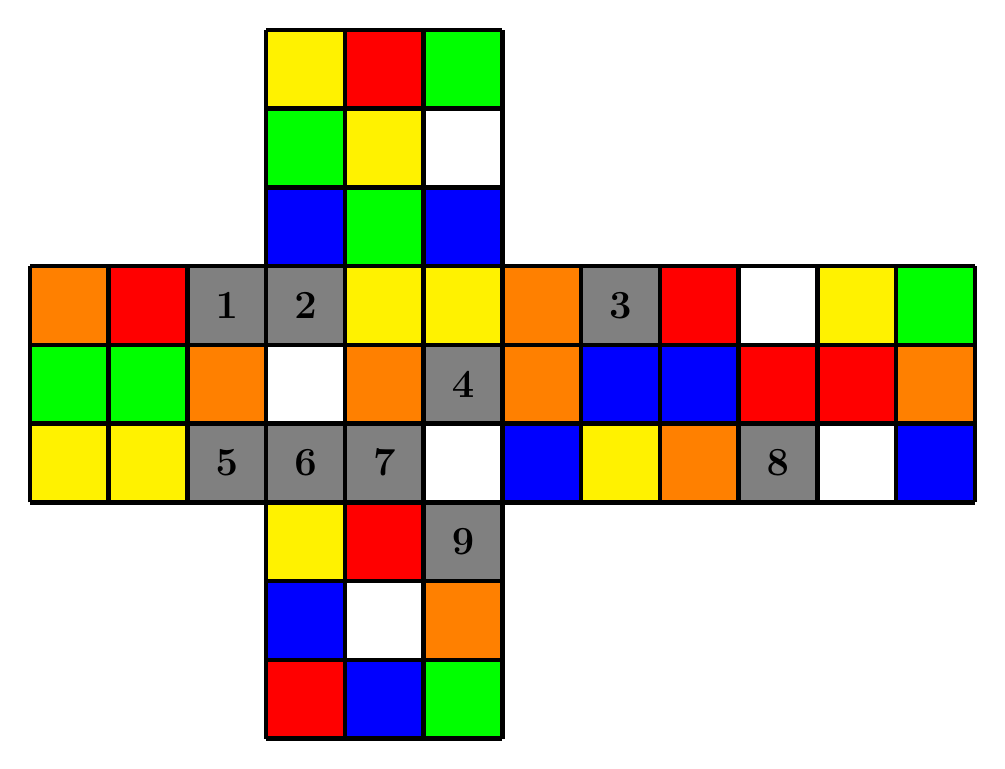
\begin{tikzpicture}[every node/.style={minimum size=1cm-\pgflinewidth, outer sep=0pt}]
\node[fill=yellow] at (0.5,5.5) {};
\node[fill=red] at (1.5,5.5) {};
\node[fill=green] at (2.5,5.5) {};
\node[fill=green] at (0.5,4.5) {};
\node[fill=yellow] at (1.5,4.5) {};
\node[fill=white] at (2.5,4.5) {};
\node[fill=blue] at (0.5,3.5) {};
\node[fill=green] at (1.5,3.5) {};
\node[fill=blue] at (2.5,3.5) {};

\node[fill=orange] at (-2.5,2.5) {};
\node[fill=red] at (-1.5,2.5) {};
\node[fill=gray] at (-0.5,2.5) {\Large \textbf 1};
\node[fill=gray] at (0.5,2.5) {\Large \textbf 2};
\node[fill=yellow] at (1.5,2.5) {};
\node[fill=yellow] at (2.5,2.5) {};
\node[fill=orange] at (3.5,2.5) {};
\node[fill=gray] at (4.5,2.5) {\Large \textbf 3};
\node[fill=red] at (5.5,2.5) {};
\node[fill=white] at (6.5,2.5) {};
\node[fill=yellow] at (7.5,2.5) {};
\node[fill=green] at (8.5,2.5) {};

\node[fill=green] at (-2.5,1.5) {};
\node[fill=green] at (-1.5,1.5) {};
\node[fill=orange] at (-0.5,1.5) {};
\node[fill=white] at (0.5,1.5) {};
\node[fill=orange] at (1.5,1.5) {};
\node[fill=gray] at (2.5,1.5) {\Large \textbf 4};
\node[fill=orange] at (3.5,1.5) {};
\node[fill=blue] at (4.5,1.5) {};
\node[fill=blue] at (5.5,1.5) {};
\node[fill=red] at (6.5,1.5) {};
\node[fill=red] at (7.5,1.5) {};
\node[fill=orange] at (8.5,1.5) {};

\node[fill=yellow] at (-2.5,0.5) {};
\node[fill=yellow] at (-1.5,0.5) {};
\node[fill=gray] at (-0.5,0.5) {\Large \textbf 5};
\node[fill=gray] at (0.5,0.5) {\Large \textbf 6};
\node[fill=gray] at (1.5,0.5) {\Large \textbf 7};
\node[fill=white] at (2.5,0.5) {};
\node[fill=blue] at (3.5,0.5) {};
\node[fill=yellow] at (4.5,0.5) {};
\node[fill=orange] at (5.5,0.5) {};
\node[fill=gray] at (6.5,0.5) {\Large \textbf 8};
\node[fill=white] at (7.5,0.5) {};
\node[fill=blue] at (8.5,0.5) {};

\node[fill=yellow] at (0.5,-0.5) {};
\node[fill=red] at (1.5,-0.5) {};
\node[fill=gray] at (2.5,-0.5) {\Large \textbf 9};
\node[fill=blue] at (0.5,-1.5) {};
\node[fill=white] at (1.5,-1.5) {};
\node[fill=orange] at (2.5,-1.5) {};
\node[fill=red] at (0.5,-2.5) {};
\node[fill=blue] at (1.5,-2.5) {};
\node[fill=green] at (2.5,-2.5) {};

\draw[step=1cm,color=black, ultra thick] (-3,0) grid (9,3);
\draw[step=1cm,color=black, ultra thick] (0,-3) grid (3,0);
\draw[step=1cm,color=black, ultra thick] (0,3) grid (3,6);
\end{tikzpicture}
\vspace{0.1cm}
\\
\noindent\normalsize \newtime  \textbf{Solution 36: B2 L' D2 U2 L' D2 R' B2 U2 L' R D' U2 B' U' F' L' R U' F' Uw2 }
\vspace{1cm}



{\noindent\Large  \newtime \textbf{No. 37\qquad Difficulty: $\bigstar\bigstar$}}
\vspace{0.2cm}\\
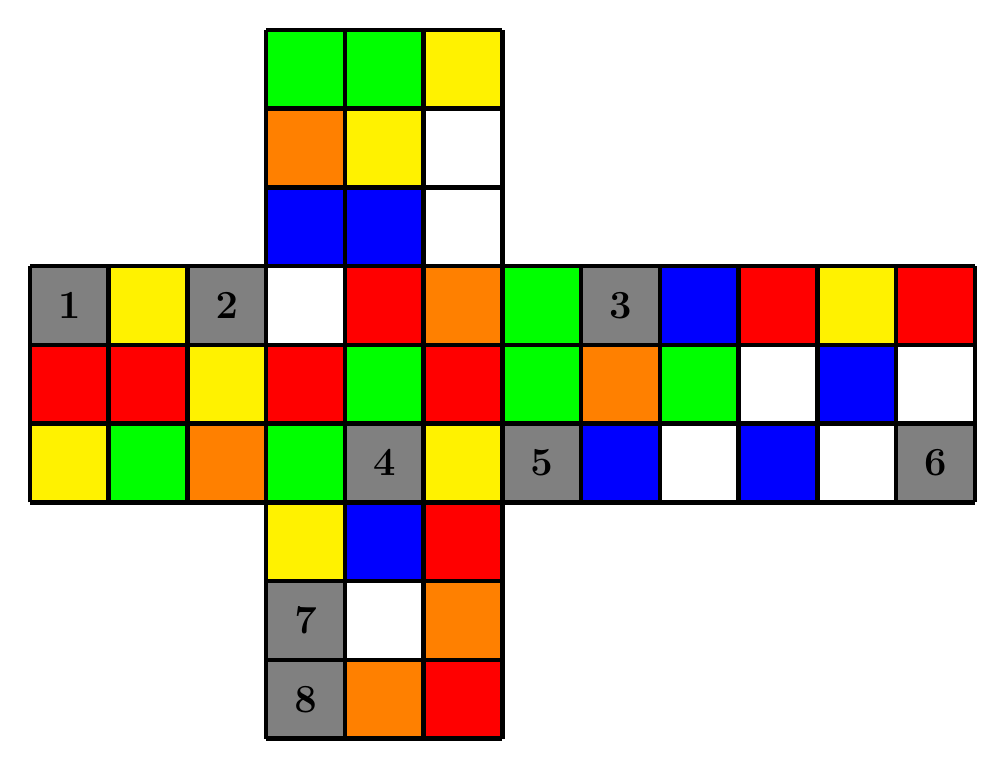
\begin{tikzpicture}[every node/.style={minimum size=1cm-\pgflinewidth, outer sep=0pt}]
\node[fill=green] at (0.5,5.5) {};
\node[fill=green] at (1.5,5.5) {};
\node[fill=yellow] at (2.5,5.5) {};
\node[fill=orange] at (0.5,4.5) {};
\node[fill=yellow] at (1.5,4.5) {};
\node[fill=white] at (2.5,4.5) {};
\node[fill=blue] at (0.5,3.5) {};
\node[fill=blue] at (1.5,3.5) {};
\node[fill=white] at (2.5,3.5) {};

\node[fill=gray] at (-2.5,2.5) {\Large \textbf 1};
\node[fill=yellow] at (-1.5,2.5) {};
\node[fill=gray] at (-0.5,2.5) {\Large \textbf 2};
\node[fill=white] at (0.5,2.5) {};
\node[fill=red] at (1.5,2.5) {};
\node[fill=orange] at (2.5,2.5) {};
\node[fill=green] at (3.5,2.5) {};
\node[fill=gray] at (4.5,2.5) {\Large \textbf 3};
\node[fill=blue] at (5.5,2.5) {};
\node[fill=red] at (6.5,2.5) {};
\node[fill=yellow] at (7.5,2.5) {};
\node[fill=red] at (8.5,2.5) {};

\node[fill=red] at (-2.5,1.5) {};
\node[fill=red] at (-1.5,1.5) {};
\node[fill=yellow] at (-0.5,1.5) {};
\node[fill=red] at (0.5,1.5) {};
\node[fill=green] at (1.5,1.5) {};
\node[fill=red] at (2.5,1.5) {};
\node[fill=green] at (3.5,1.5) {};
\node[fill=orange] at (4.5,1.5) {};
\node[fill=green] at (5.5,1.5) {};
\node[fill=white] at (6.5,1.5) {};
\node[fill=blue] at (7.5,1.5) {};
\node[fill=white] at (8.5,1.5) {};

\node[fill=yellow] at (-2.5,0.5) {};
\node[fill=green] at (-1.5,0.5) {};
\node[fill=orange] at (-0.5,0.5) {};
\node[fill=green] at (0.5,0.5) {};
\node[fill=gray] at (1.5,0.5) {\Large \textbf 4};
\node[fill=yellow] at (2.5,0.5) {};
\node[fill=gray] at (3.5,0.5) {\Large \textbf 5};
\node[fill=blue] at (4.5,0.5) {};
\node[fill=white] at (5.5,0.5) {};
\node[fill=blue] at (6.5,0.5) {};
\node[fill=white] at (7.5,0.5) {};
\node[fill=gray] at (8.5,0.5) {\Large \textbf 6};

\node[fill=yellow] at (0.5,-0.5) {};
\node[fill=blue] at (1.5,-0.5) {};
\node[fill=red] at (2.5,-0.5) {};
\node[fill=gray] at (0.5,-1.5) {\Large \textbf 7};
\node[fill=white] at (1.5,-1.5) {};
\node[fill=orange] at (2.5,-1.5) {};
\node[fill=gray] at (0.5,-2.5) {\Large \textbf 8};
\node[fill=orange] at (1.5,-2.5) {};
\node[fill=red] at (2.5,-2.5) {};

\draw[step=1cm,color=black, ultra thick] (-3,0) grid (9,3);
\draw[step=1cm,color=black, ultra thick] (0,-3) grid (3,0);
\draw[step=1cm,color=black, ultra thick] (0,3) grid (3,6);
\end{tikzpicture}
\vspace{0.1cm}
\\
\noindent\normalsize \newtime  \textbf{Solution 37: D' B2 R' U L2 U B' L F' B' L2 F' D' B' F' D' L2 R' F R' Uw }
\vspace{1cm}



{\noindent\Large  \newtime \textbf{No. 38\qquad Difficulty: $\bigstar\bigstar$}}
\vspace{0.2cm}\\
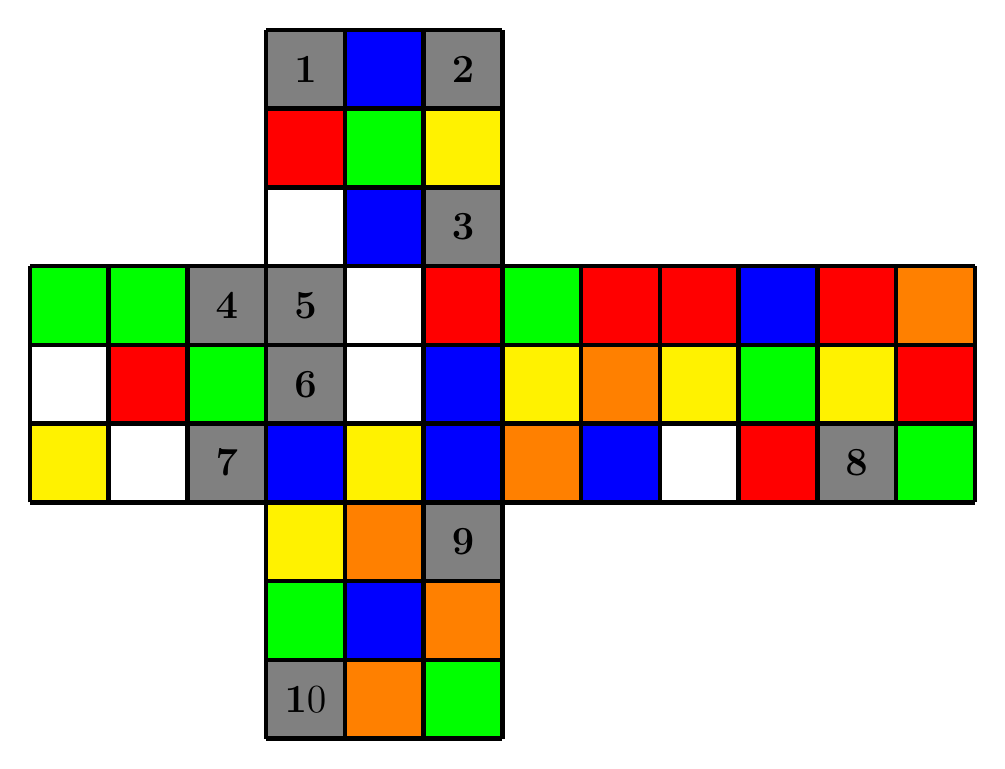
\begin{tikzpicture}[every node/.style={minimum size=1cm-\pgflinewidth, outer sep=0pt}]
\node[fill=gray] at (0.5,5.5) {\Large \textbf 1};
\node[fill=blue] at (1.5,5.5) {};
\node[fill=gray] at (2.5,5.5) {\Large \textbf 2};
\node[fill=red] at (0.5,4.5) {};
\node[fill=green] at (1.5,4.5) {};
\node[fill=yellow] at (2.5,4.5) {};
\node[fill=white] at (0.5,3.5) {};
\node[fill=blue] at (1.5,3.5) {};
\node[fill=gray] at (2.5,3.5) {\Large \textbf 3};

\node[fill=green] at (-2.5,2.5) {};
\node[fill=green] at (-1.5,2.5) {};
\node[fill=gray] at (-0.5,2.5) {\Large \textbf 4};
\node[fill=gray] at (0.5,2.5) {\Large \textbf 5};
\node[fill=white] at (1.5,2.5) {};
\node[fill=red] at (2.5,2.5) {};
\node[fill=green] at (3.5,2.5) {};
\node[fill=red] at (4.5,2.5) {};
\node[fill=red] at (5.5,2.5) {};
\node[fill=blue] at (6.5,2.5) {};
\node[fill=red] at (7.5,2.5) {};
\node[fill=orange] at (8.5,2.5) {};

\node[fill=white] at (-2.5,1.5) {};
\node[fill=red] at (-1.5,1.5) {};
\node[fill=green] at (-0.5,1.5) {};
\node[fill=gray] at (0.5,1.5) {\Large \textbf 6};
\node[fill=white] at (1.5,1.5) {};
\node[fill=blue] at (2.5,1.5) {};
\node[fill=yellow] at (3.5,1.5) {};
\node[fill=orange] at (4.5,1.5) {};
\node[fill=yellow] at (5.5,1.5) {};
\node[fill=green] at (6.5,1.5) {};
\node[fill=yellow] at (7.5,1.5) {};
\node[fill=red] at (8.5,1.5) {};

\node[fill=yellow] at (-2.5,0.5) {};
\node[fill=white] at (-1.5,0.5) {};
\node[fill=gray] at (-0.5,0.5) {\Large \textbf 7};
\node[fill=blue] at (0.5,0.5) {};
\node[fill=yellow] at (1.5,0.5) {};
\node[fill=blue] at (2.5,0.5) {};
\node[fill=orange] at (3.5,0.5) {};
\node[fill=blue] at (4.5,0.5) {};
\node[fill=white] at (5.5,0.5) {};
\node[fill=red] at (6.5,0.5) {};
\node[fill=gray] at (7.5,0.5) {\Large \textbf 8};
\node[fill=green] at (8.5,0.5) {};

\node[fill=yellow] at (0.5,-0.5) {};
\node[fill=orange] at (1.5,-0.5) {};
\node[fill=gray] at (2.5,-0.5) {\Large \textbf 9};
\node[fill=green] at (0.5,-1.5) {};
\node[fill=blue] at (1.5,-1.5) {};
\node[fill=orange] at (2.5,-1.5) {};
\node[fill=gray] at (0.5,-2.5) {\Large \textbf 10};
\node[fill=orange] at (1.5,-2.5) {};
\node[fill=green] at (2.5,-2.5) {};

\draw[step=1cm,color=black, ultra thick] (-3,0) grid (9,3);
\draw[step=1cm,color=black, ultra thick] (0,-3) grid (3,0);
\draw[step=1cm,color=black, ultra thick] (0,3) grid (3,6);
\end{tikzpicture}
\vspace{0.1cm}
\\
\noindent\normalsize \newtime  \textbf{Solution 38: B' R2 U D' B2 D' U' L2 U R U R2 B2 L' F2 U' R' L B2 F Fw' Uw }
\vspace{1cm}



{\noindent\Large  \newtime \textbf{No. 39\qquad Difficulty: $\bigstar\bigstar$}}
\vspace{0.2cm}\\
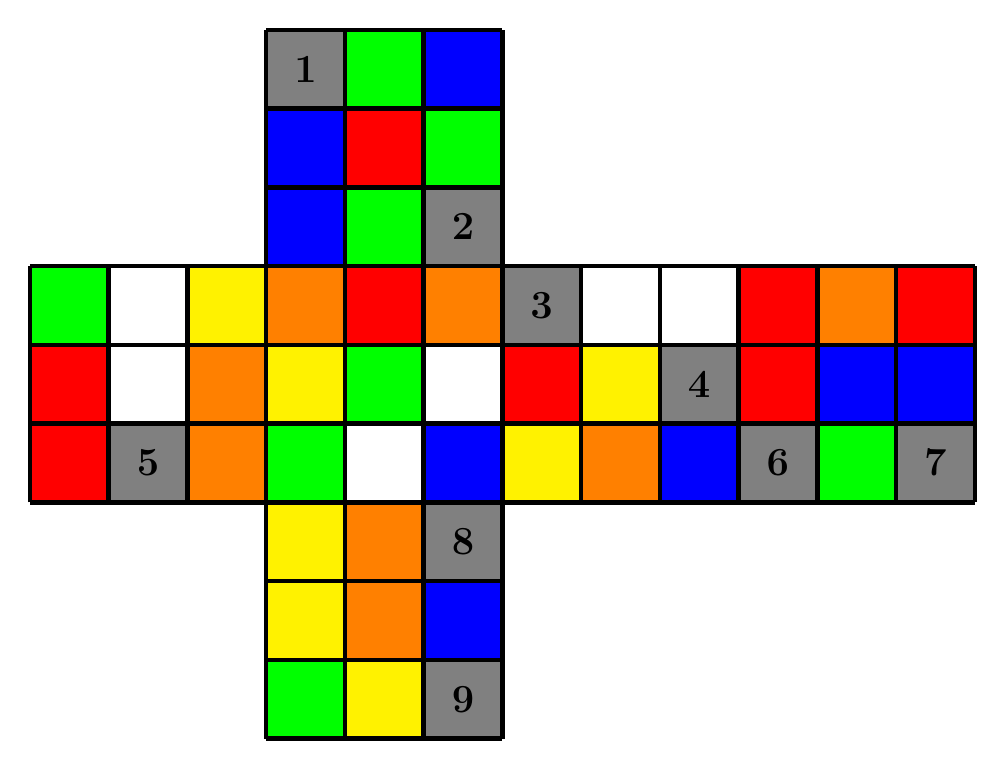
\begin{tikzpicture}[every node/.style={minimum size=1cm-\pgflinewidth, outer sep=0pt}]
\node[fill=gray] at (0.5,5.5) {\Large \textbf 1};
\node[fill=green] at (1.5,5.5) {};
\node[fill=blue] at (2.5,5.5) {};
\node[fill=blue] at (0.5,4.5) {};
\node[fill=red] at (1.5,4.5) {};
\node[fill=green] at (2.5,4.5) {};
\node[fill=blue] at (0.5,3.5) {};
\node[fill=green] at (1.5,3.5) {};
\node[fill=gray] at (2.5,3.5) {\Large \textbf 2};

\node[fill=green] at (-2.5,2.5) {};
\node[fill=white] at (-1.5,2.5) {};
\node[fill=yellow] at (-0.5,2.5) {};
\node[fill=orange] at (0.5,2.5) {};
\node[fill=red] at (1.5,2.5) {};
\node[fill=orange] at (2.5,2.5) {};
\node[fill=gray] at (3.5,2.5) {\Large \textbf 3};
\node[fill=white] at (4.5,2.5) {};
\node[fill=white] at (5.5,2.5) {};
\node[fill=red] at (6.5,2.5) {};
\node[fill=orange] at (7.5,2.5) {};
\node[fill=red] at (8.5,2.5) {};

\node[fill=red] at (-2.5,1.5) {};
\node[fill=white] at (-1.5,1.5) {};
\node[fill=orange] at (-0.5,1.5) {};
\node[fill=yellow] at (0.5,1.5) {};
\node[fill=green] at (1.5,1.5) {};
\node[fill=white] at (2.5,1.5) {};
\node[fill=red] at (3.5,1.5) {};
\node[fill=yellow] at (4.5,1.5) {};
\node[fill=gray] at (5.5,1.5) {\Large \textbf 4};
\node[fill=red] at (6.5,1.5) {};
\node[fill=blue] at (7.5,1.5) {};
\node[fill=blue] at (8.5,1.5) {};

\node[fill=red] at (-2.5,0.5) {};
\node[fill=gray] at (-1.5,0.5) {\Large \textbf 5};
\node[fill=orange] at (-0.5,0.5) {};
\node[fill=green] at (0.5,0.5) {};
\node[fill=white] at (1.5,0.5) {};
\node[fill=blue] at (2.5,0.5) {};
\node[fill=yellow] at (3.5,0.5) {};
\node[fill=orange] at (4.5,0.5) {};
\node[fill=blue] at (5.5,0.5) {};
\node[fill=gray] at (6.5,0.5) {\Large \textbf 6};
\node[fill=green] at (7.5,0.5) {};
\node[fill=gray] at (8.5,0.5) {\Large \textbf 7};

\node[fill=yellow] at (0.5,-0.5) {};
\node[fill=orange] at (1.5,-0.5) {};
\node[fill=gray] at (2.5,-0.5) {\Large \textbf 8};
\node[fill=yellow] at (0.5,-1.5) {};
\node[fill=orange] at (1.5,-1.5) {};
\node[fill=blue] at (2.5,-1.5) {};
\node[fill=green] at (0.5,-2.5) {};
\node[fill=yellow] at (1.5,-2.5) {};
\node[fill=gray] at (2.5,-2.5) {\Large \textbf 9};

\draw[step=1cm,color=black, ultra thick] (-3,0) grid (9,3);
\draw[step=1cm,color=black, ultra thick] (0,-3) grid (3,0);
\draw[step=1cm,color=black, ultra thick] (0,3) grid (3,6);
\end{tikzpicture}
\vspace{0.1cm}
\\
\noindent\normalsize \newtime  \textbf{Solution 39: U B R2 B2 F L2 D' R2 F' L2 D' R2 D' F2 L' U2 L' U' D' R Rw Uw }
\vspace{1cm}



{\noindent\Large  \newtime \textbf{No. 40\qquad Difficulty: $\bigstar\bigstar$}}
\vspace{0.2cm}\\
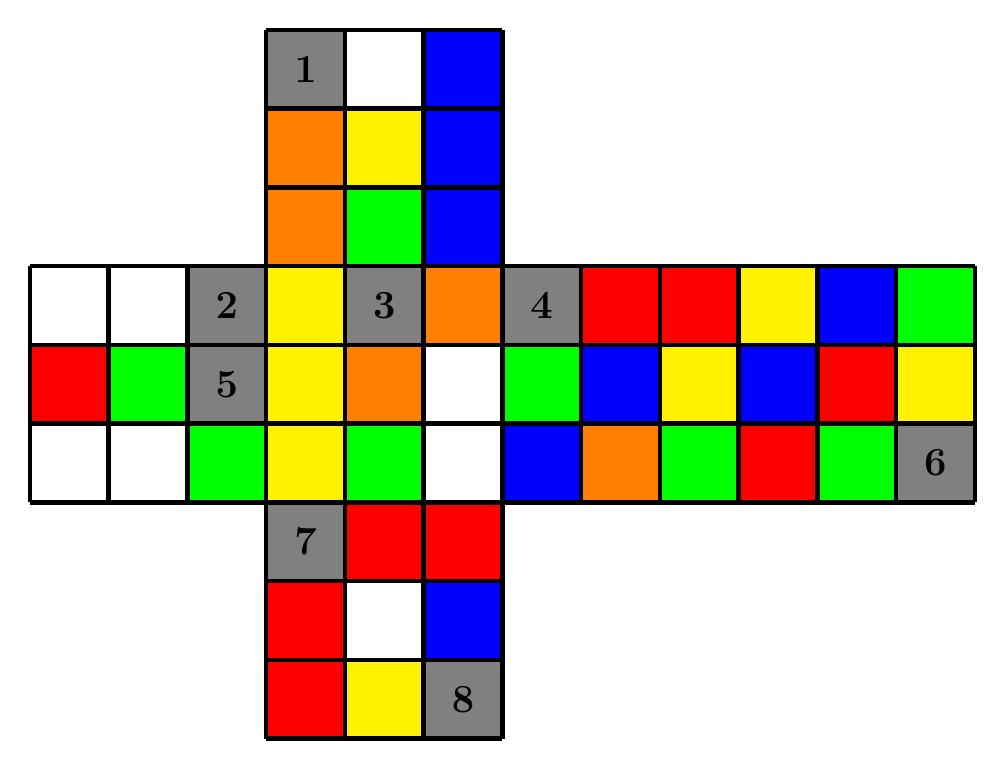
\begin{tikzpicture}[every node/.style={minimum size=1cm-\pgflinewidth, outer sep=0pt}]
\node[fill=gray] at (0.5,5.5) {\Large \textbf 1};
\node[fill=white] at (1.5,5.5) {};
\node[fill=blue] at (2.5,5.5) {};
\node[fill=orange] at (0.5,4.5) {};
\node[fill=yellow] at (1.5,4.5) {};
\node[fill=blue] at (2.5,4.5) {};
\node[fill=orange] at (0.5,3.5) {};
\node[fill=green] at (1.5,3.5) {};
\node[fill=blue] at (2.5,3.5) {};

\node[fill=white] at (-2.5,2.5) {};
\node[fill=white] at (-1.5,2.5) {};
\node[fill=gray] at (-0.5,2.5) {\Large \textbf 2};
\node[fill=yellow] at (0.5,2.5) {};
\node[fill=gray] at (1.5,2.5) {\Large \textbf 3};
\node[fill=orange] at (2.5,2.5) {};
\node[fill=gray] at (3.5,2.5) {\Large \textbf 4};
\node[fill=red] at (4.5,2.5) {};
\node[fill=red] at (5.5,2.5) {};
\node[fill=yellow] at (6.5,2.5) {};
\node[fill=blue] at (7.5,2.5) {};
\node[fill=green] at (8.5,2.5) {};

\node[fill=red] at (-2.5,1.5) {};
\node[fill=green] at (-1.5,1.5) {};
\node[fill=gray] at (-0.5,1.5) {\Large \textbf 5};
\node[fill=yellow] at (0.5,1.5) {};
\node[fill=orange] at (1.5,1.5) {};
\node[fill=white] at (2.5,1.5) {};
\node[fill=green] at (3.5,1.5) {};
\node[fill=blue] at (4.5,1.5) {};
\node[fill=yellow] at (5.5,1.5) {};
\node[fill=blue] at (6.5,1.5) {};
\node[fill=red] at (7.5,1.5) {};
\node[fill=yellow] at (8.5,1.5) {};

\node[fill=white] at (-2.5,0.5) {};
\node[fill=white] at (-1.5,0.5) {};
\node[fill=green] at (-0.5,0.5) {};
\node[fill=yellow] at (0.5,0.5) {};
\node[fill=green] at (1.5,0.5) {};
\node[fill=white] at (2.5,0.5) {};
\node[fill=blue] at (3.5,0.5) {};
\node[fill=orange] at (4.5,0.5) {};
\node[fill=green] at (5.5,0.5) {};
\node[fill=red] at (6.5,0.5) {};
\node[fill=green] at (7.5,0.5) {};
\node[fill=gray] at (8.5,0.5) {\Large \textbf 6};

\node[fill=gray] at (0.5,-0.5) {\Large \textbf 7};
\node[fill=red] at (1.5,-0.5) {};
\node[fill=red] at (2.5,-0.5) {};
\node[fill=red] at (0.5,-1.5) {};
\node[fill=white] at (1.5,-1.5) {};
\node[fill=blue] at (2.5,-1.5) {};
\node[fill=red] at (0.5,-2.5) {};
\node[fill=yellow] at (1.5,-2.5) {};
\node[fill=gray] at (2.5,-2.5) {\Large \textbf 8};

\draw[step=1cm,color=black, ultra thick] (-3,0) grid (9,3);
\draw[step=1cm,color=black, ultra thick] (0,-3) grid (3,0);
\draw[step=1cm,color=black, ultra thick] (0,3) grid (3,6);
\end{tikzpicture}
\vspace{0.1cm}
\\
\noindent\normalsize \newtime  \textbf{Solution 40: U2 F D2 U L R2 F L' U' B U R D' B' U2 B' D' B2 D L Uw2 }
\vspace{1cm}



{\noindent\Large  \newtime \textbf{No. 41\qquad Difficulty: $\bigstar\bigstar$}}
\vspace{0.2cm}\\
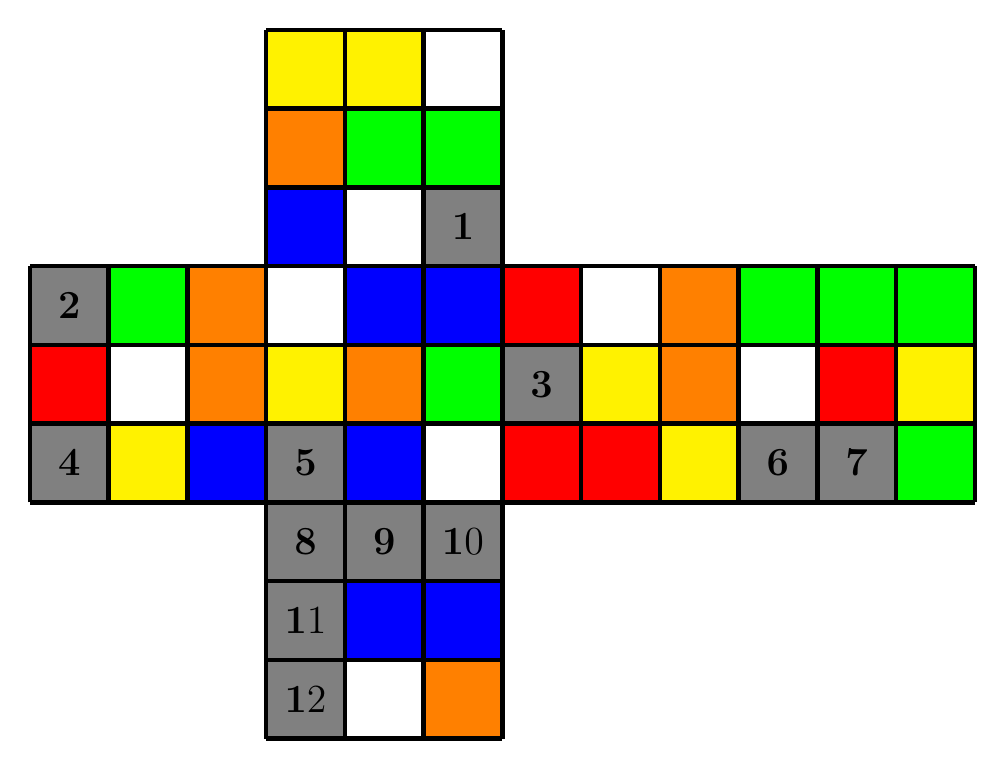
\begin{tikzpicture}[every node/.style={minimum size=1cm-\pgflinewidth, outer sep=0pt}]
\node[fill=yellow] at (0.5,5.5) {};
\node[fill=yellow] at (1.5,5.5) {};
\node[fill=white] at (2.5,5.5) {};
\node[fill=orange] at (0.5,4.5) {};
\node[fill=green] at (1.5,4.5) {};
\node[fill=green] at (2.5,4.5) {};
\node[fill=blue] at (0.5,3.5) {};
\node[fill=white] at (1.5,3.5) {};
\node[fill=gray] at (2.5,3.5) {\Large \textbf 1};

\node[fill=gray] at (-2.5,2.5) {\Large \textbf 2};
\node[fill=green] at (-1.5,2.5) {};
\node[fill=orange] at (-0.5,2.5) {};
\node[fill=white] at (0.5,2.5) {};
\node[fill=blue] at (1.5,2.5) {};
\node[fill=blue] at (2.5,2.5) {};
\node[fill=red] at (3.5,2.5) {};
\node[fill=white] at (4.5,2.5) {};
\node[fill=orange] at (5.5,2.5) {};
\node[fill=green] at (6.5,2.5) {};
\node[fill=green] at (7.5,2.5) {};
\node[fill=green] at (8.5,2.5) {};

\node[fill=red] at (-2.5,1.5) {};
\node[fill=white] at (-1.5,1.5) {};
\node[fill=orange] at (-0.5,1.5) {};
\node[fill=yellow] at (0.5,1.5) {};
\node[fill=orange] at (1.5,1.5) {};
\node[fill=green] at (2.5,1.5) {};
\node[fill=gray] at (3.5,1.5) {\Large \textbf 3};
\node[fill=yellow] at (4.5,1.5) {};
\node[fill=orange] at (5.5,1.5) {};
\node[fill=white] at (6.5,1.5) {};
\node[fill=red] at (7.5,1.5) {};
\node[fill=yellow] at (8.5,1.5) {};

\node[fill=gray] at (-2.5,0.5) {\Large \textbf 4};
\node[fill=yellow] at (-1.5,0.5) {};
\node[fill=blue] at (-0.5,0.5) {};
\node[fill=gray] at (0.5,0.5) {\Large \textbf 5};
\node[fill=blue] at (1.5,0.5) {};
\node[fill=white] at (2.5,0.5) {};
\node[fill=red] at (3.5,0.5) {};
\node[fill=red] at (4.5,0.5) {};
\node[fill=yellow] at (5.5,0.5) {};
\node[fill=gray] at (6.5,0.5) {\Large \textbf 6};
\node[fill=gray] at (7.5,0.5) {\Large \textbf 7};
\node[fill=green] at (8.5,0.5) {};

\node[fill=gray] at (0.5,-0.5) {\Large \textbf 8};
\node[fill=gray] at (1.5,-0.5) {\Large \textbf 9};
\node[fill=gray] at (2.5,-0.5) {\Large \textbf 10};
\node[fill=gray] at (0.5,-1.5) {\Large \textbf 11};
\node[fill=blue] at (1.5,-1.5) {};
\node[fill=blue] at (2.5,-1.5) {};
\node[fill=gray] at (0.5,-2.5) {\Large \textbf 12};
\node[fill=white] at (1.5,-2.5) {};
\node[fill=orange] at (2.5,-2.5) {};

\draw[step=1cm,color=black, ultra thick] (-3,0) grid (9,3);
\draw[step=1cm,color=black, ultra thick] (0,-3) grid (3,0);
\draw[step=1cm,color=black, ultra thick] (0,3) grid (3,6);
\end{tikzpicture}
\vspace{0.1cm}
\\
\noindent\normalsize \newtime  \textbf{Solution 41: D' L R2 B L' D U2 R U' L R' F' L' U' L F U' B F' R2 Fw' Uw2 }
\vspace{1cm}



{\noindent\Large  \newtime \textbf{No. 42\qquad Difficulty: $\bigstar\bigstar$}}
\vspace{0.2cm}\\
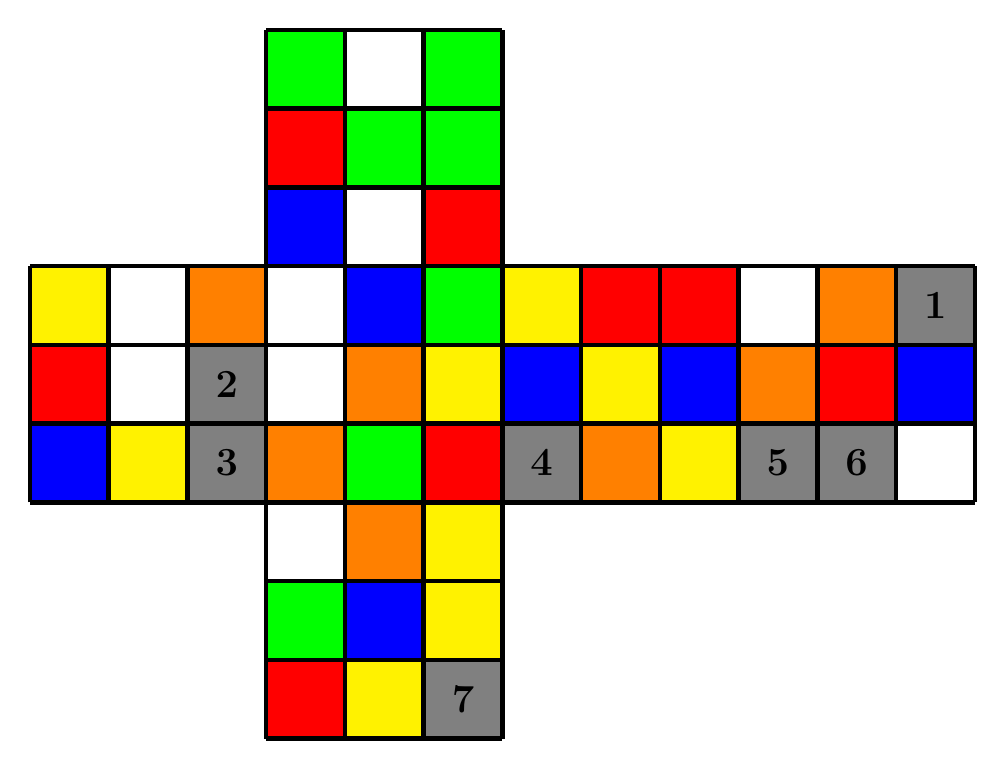
\begin{tikzpicture}[every node/.style={minimum size=1cm-\pgflinewidth, outer sep=0pt}]
\node[fill=green] at (0.5,5.5) {};
\node[fill=white] at (1.5,5.5) {};
\node[fill=green] at (2.5,5.5) {};
\node[fill=red] at (0.5,4.5) {};
\node[fill=green] at (1.5,4.5) {};
\node[fill=green] at (2.5,4.5) {};
\node[fill=blue] at (0.5,3.5) {};
\node[fill=white] at (1.5,3.5) {};
\node[fill=red] at (2.5,3.5) {};

\node[fill=yellow] at (-2.5,2.5) {};
\node[fill=white] at (-1.5,2.5) {};
\node[fill=orange] at (-0.5,2.5) {};
\node[fill=white] at (0.5,2.5) {};
\node[fill=blue] at (1.5,2.5) {};
\node[fill=green] at (2.5,2.5) {};
\node[fill=yellow] at (3.5,2.5) {};
\node[fill=red] at (4.5,2.5) {};
\node[fill=red] at (5.5,2.5) {};
\node[fill=white] at (6.5,2.5) {};
\node[fill=orange] at (7.5,2.5) {};
\node[fill=gray] at (8.5,2.5) {\Large \textbf 1};

\node[fill=red] at (-2.5,1.5) {};
\node[fill=white] at (-1.5,1.5) {};
\node[fill=gray] at (-0.5,1.5) {\Large \textbf 2};
\node[fill=white] at (0.5,1.5) {};
\node[fill=orange] at (1.5,1.5) {};
\node[fill=yellow] at (2.5,1.5) {};
\node[fill=blue] at (3.5,1.5) {};
\node[fill=yellow] at (4.5,1.5) {};
\node[fill=blue] at (5.5,1.5) {};
\node[fill=orange] at (6.5,1.5) {};
\node[fill=red] at (7.5,1.5) {};
\node[fill=blue] at (8.5,1.5) {};

\node[fill=blue] at (-2.5,0.5) {};
\node[fill=yellow] at (-1.5,0.5) {};
\node[fill=gray] at (-0.5,0.5) {\Large \textbf 3};
\node[fill=orange] at (0.5,0.5) {};
\node[fill=green] at (1.5,0.5) {};
\node[fill=red] at (2.5,0.5) {};
\node[fill=gray] at (3.5,0.5) {\Large \textbf 4};
\node[fill=orange] at (4.5,0.5) {};
\node[fill=yellow] at (5.5,0.5) {};
\node[fill=gray] at (6.5,0.5) {\Large \textbf 5};
\node[fill=gray] at (7.5,0.5) {\Large \textbf 6};
\node[fill=white] at (8.5,0.5) {};

\node[fill=white] at (0.5,-0.5) {};
\node[fill=orange] at (1.5,-0.5) {};
\node[fill=yellow] at (2.5,-0.5) {};
\node[fill=green] at (0.5,-1.5) {};
\node[fill=blue] at (1.5,-1.5) {};
\node[fill=yellow] at (2.5,-1.5) {};
\node[fill=red] at (0.5,-2.5) {};
\node[fill=yellow] at (1.5,-2.5) {};
\node[fill=gray] at (2.5,-2.5) {\Large \textbf 7};

\draw[step=1cm,color=black, ultra thick] (-3,0) grid (9,3);
\draw[step=1cm,color=black, ultra thick] (0,-3) grid (3,0);
\draw[step=1cm,color=black, ultra thick] (0,3) grid (3,6);
\end{tikzpicture}
\vspace{0.1cm}
\\
\noindent\normalsize \newtime  \textbf{Solution 42: B' L2 B' U2 F2 L' U B2 R2 D B' R' L2 D2 F' R2 D2 F R2 U2 Fw' Uw2 }
\vspace{1cm}



{\noindent\Large  \newtime \textbf{No. 43\qquad Difficulty: $\bigstar\bigstar$}}
\vspace{0.2cm}\\
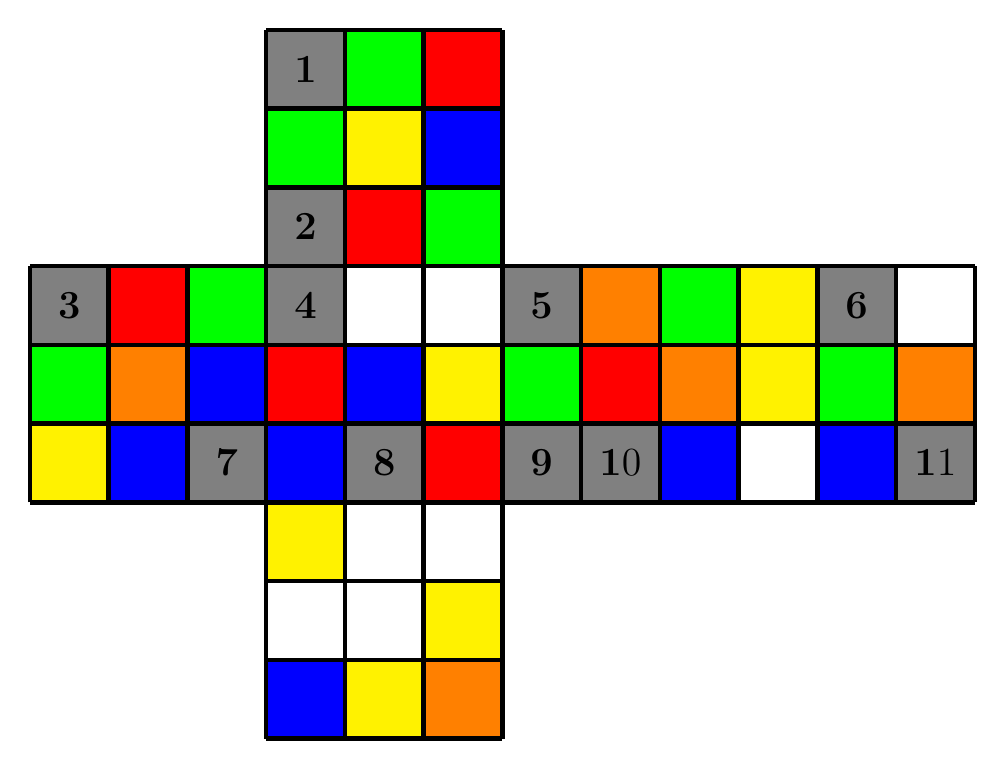
\begin{tikzpicture}[every node/.style={minimum size=1cm-\pgflinewidth, outer sep=0pt}]
\node[fill=gray] at (0.5,5.5) {\Large \textbf 1};
\node[fill=green] at (1.5,5.5) {};
\node[fill=red] at (2.5,5.5) {};
\node[fill=green] at (0.5,4.5) {};
\node[fill=yellow] at (1.5,4.5) {};
\node[fill=blue] at (2.5,4.5) {};
\node[fill=gray] at (0.5,3.5) {\Large \textbf 2};
\node[fill=red] at (1.5,3.5) {};
\node[fill=green] at (2.5,3.5) {};

\node[fill=gray] at (-2.5,2.5) {\Large \textbf 3};
\node[fill=red] at (-1.5,2.5) {};
\node[fill=green] at (-0.5,2.5) {};
\node[fill=gray] at (0.5,2.5) {\Large \textbf 4};
\node[fill=white] at (1.5,2.5) {};
\node[fill=white] at (2.5,2.5) {};
\node[fill=gray] at (3.5,2.5) {\Large \textbf 5};
\node[fill=orange] at (4.5,2.5) {};
\node[fill=green] at (5.5,2.5) {};
\node[fill=yellow] at (6.5,2.5) {};
\node[fill=gray] at (7.5,2.5) {\Large \textbf 6};
\node[fill=white] at (8.5,2.5) {};

\node[fill=green] at (-2.5,1.5) {};
\node[fill=orange] at (-1.5,1.5) {};
\node[fill=blue] at (-0.5,1.5) {};
\node[fill=red] at (0.5,1.5) {};
\node[fill=blue] at (1.5,1.5) {};
\node[fill=yellow] at (2.5,1.5) {};
\node[fill=green] at (3.5,1.5) {};
\node[fill=red] at (4.5,1.5) {};
\node[fill=orange] at (5.5,1.5) {};
\node[fill=yellow] at (6.5,1.5) {};
\node[fill=green] at (7.5,1.5) {};
\node[fill=orange] at (8.5,1.5) {};

\node[fill=yellow] at (-2.5,0.5) {};
\node[fill=blue] at (-1.5,0.5) {};
\node[fill=gray] at (-0.5,0.5) {\Large \textbf 7};
\node[fill=blue] at (0.5,0.5) {};
\node[fill=gray] at (1.5,0.5) {\Large \textbf 8};
\node[fill=red] at (2.5,0.5) {};
\node[fill=gray] at (3.5,0.5) {\Large \textbf 9};
\node[fill=gray] at (4.5,0.5) {\Large \textbf 10};
\node[fill=blue] at (5.5,0.5) {};
\node[fill=white] at (6.5,0.5) {};
\node[fill=blue] at (7.5,0.5) {};
\node[fill=gray] at (8.5,0.5) {\Large \textbf 11};

\node[fill=yellow] at (0.5,-0.5) {};
\node[fill=white] at (1.5,-0.5) {};
\node[fill=white] at (2.5,-0.5) {};
\node[fill=white] at (0.5,-1.5) {};
\node[fill=white] at (1.5,-1.5) {};
\node[fill=yellow] at (2.5,-1.5) {};
\node[fill=blue] at (0.5,-2.5) {};
\node[fill=yellow] at (1.5,-2.5) {};
\node[fill=orange] at (2.5,-2.5) {};

\draw[step=1cm,color=black, ultra thick] (-3,0) grid (9,3);
\draw[step=1cm,color=black, ultra thick] (0,-3) grid (3,0);
\draw[step=1cm,color=black, ultra thick] (0,3) grid (3,6);
\end{tikzpicture}
\vspace{0.1cm}
\\
\noindent\normalsize \newtime  \textbf{Solution 43: D B' F' D' R2 L' U2 L' B2 L' D2 F2 B R' B' F D F' U2 F2 Uw' }
\vspace{1cm}



{\noindent\Large  \newtime \textbf{No. 44\qquad Difficulty: $\bigstar\bigstar$}}
\vspace{0.2cm}\\
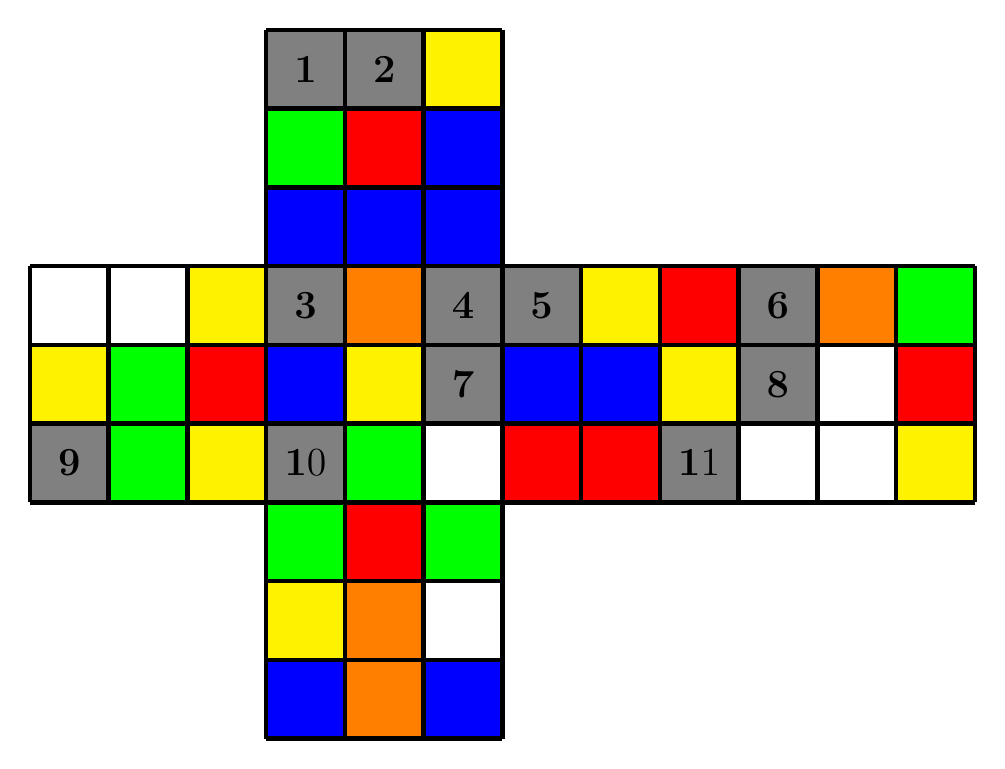
\begin{tikzpicture}[every node/.style={minimum size=1cm-\pgflinewidth, outer sep=0pt}]
\node[fill=gray] at (0.5,5.5) {\Large \textbf 1};
\node[fill=gray] at (1.5,5.5) {\Large \textbf 2};
\node[fill=yellow] at (2.5,5.5) {};
\node[fill=green] at (0.5,4.5) {};
\node[fill=red] at (1.5,4.5) {};
\node[fill=blue] at (2.5,4.5) {};
\node[fill=blue] at (0.5,3.5) {};
\node[fill=blue] at (1.5,3.5) {};
\node[fill=blue] at (2.5,3.5) {};

\node[fill=white] at (-2.5,2.5) {};
\node[fill=white] at (-1.5,2.5) {};
\node[fill=yellow] at (-0.5,2.5) {};
\node[fill=gray] at (0.5,2.5) {\Large \textbf 3};
\node[fill=orange] at (1.5,2.5) {};
\node[fill=gray] at (2.5,2.5) {\Large \textbf 4};
\node[fill=gray] at (3.5,2.5) {\Large \textbf 5};
\node[fill=yellow] at (4.5,2.5) {};
\node[fill=red] at (5.5,2.5) {};
\node[fill=gray] at (6.5,2.5) {\Large \textbf 6};
\node[fill=orange] at (7.5,2.5) {};
\node[fill=green] at (8.5,2.5) {};

\node[fill=yellow] at (-2.5,1.5) {};
\node[fill=green] at (-1.5,1.5) {};
\node[fill=red] at (-0.5,1.5) {};
\node[fill=blue] at (0.5,1.5) {};
\node[fill=yellow] at (1.5,1.5) {};
\node[fill=gray] at (2.5,1.5) {\Large \textbf 7};
\node[fill=blue] at (3.5,1.5) {};
\node[fill=blue] at (4.5,1.5) {};
\node[fill=yellow] at (5.5,1.5) {};
\node[fill=gray] at (6.5,1.5) {\Large \textbf 8};
\node[fill=white] at (7.5,1.5) {};
\node[fill=red] at (8.5,1.5) {};

\node[fill=gray] at (-2.5,0.5) {\Large \textbf 9};
\node[fill=green] at (-1.5,0.5) {};
\node[fill=yellow] at (-0.5,0.5) {};
\node[fill=gray] at (0.5,0.5) {\Large \textbf 10};
\node[fill=green] at (1.5,0.5) {};
\node[fill=white] at (2.5,0.5) {};
\node[fill=red] at (3.5,0.5) {};
\node[fill=red] at (4.5,0.5) {};
\node[fill=gray] at (5.5,0.5) {\Large \textbf 11};
\node[fill=white] at (6.5,0.5) {};
\node[fill=white] at (7.5,0.5) {};
\node[fill=yellow] at (8.5,0.5) {};

\node[fill=green] at (0.5,-0.5) {};
\node[fill=red] at (1.5,-0.5) {};
\node[fill=green] at (2.5,-0.5) {};
\node[fill=yellow] at (0.5,-1.5) {};
\node[fill=orange] at (1.5,-1.5) {};
\node[fill=white] at (2.5,-1.5) {};
\node[fill=blue] at (0.5,-2.5) {};
\node[fill=orange] at (1.5,-2.5) {};
\node[fill=blue] at (2.5,-2.5) {};

\draw[step=1cm,color=black, ultra thick] (-3,0) grid (9,3);
\draw[step=1cm,color=black, ultra thick] (0,-3) grid (3,0);
\draw[step=1cm,color=black, ultra thick] (0,3) grid (3,6);
\end{tikzpicture}
\vspace{0.1cm}
\\
\noindent\normalsize \newtime  \textbf{Solution 44: L' F2 L F R2 D2 R B' D B L D2 U2 F' L2 D' F2 U L2 D2 Rw Uw2 }
\vspace{1cm}



{\noindent\Large  \newtime \textbf{No. 45\qquad Difficulty: $\bigstar\bigstar$}}
\vspace{0.2cm}\\
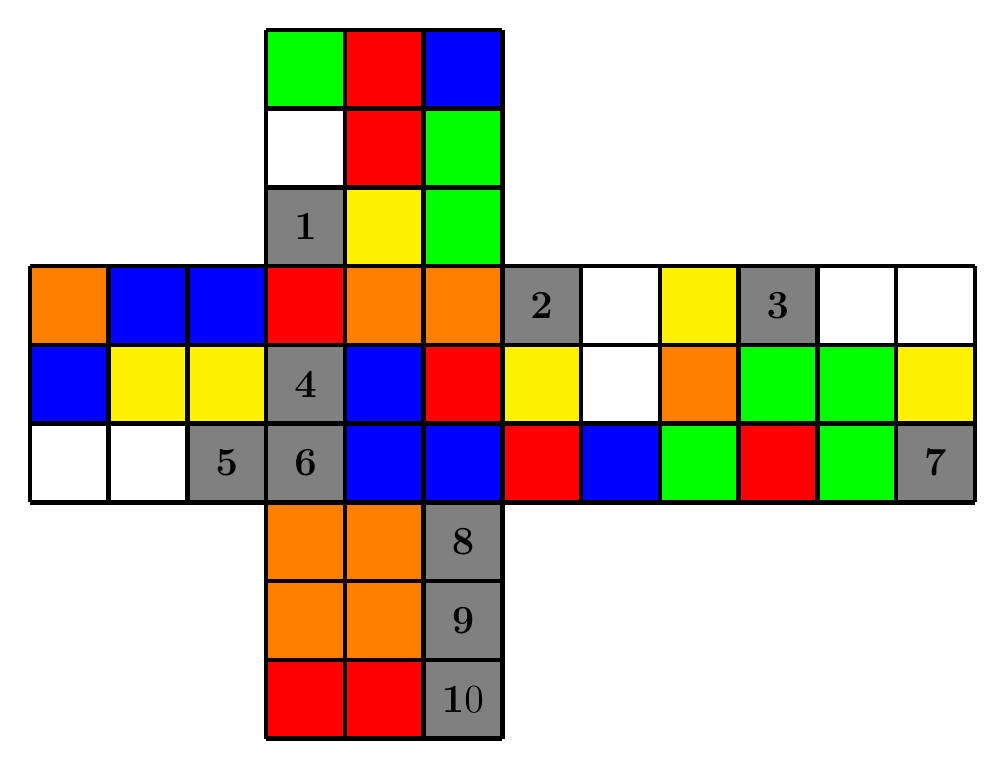
\begin{tikzpicture}[every node/.style={minimum size=1cm-\pgflinewidth, outer sep=0pt}]
\node[fill=green] at (0.5,5.5) {};
\node[fill=red] at (1.5,5.5) {};
\node[fill=blue] at (2.5,5.5) {};
\node[fill=white] at (0.5,4.5) {};
\node[fill=red] at (1.5,4.5) {};
\node[fill=green] at (2.5,4.5) {};
\node[fill=gray] at (0.5,3.5) {\Large \textbf 1};
\node[fill=yellow] at (1.5,3.5) {};
\node[fill=green] at (2.5,3.5) {};

\node[fill=orange] at (-2.5,2.5) {};
\node[fill=blue] at (-1.5,2.5) {};
\node[fill=blue] at (-0.5,2.5) {};
\node[fill=red] at (0.5,2.5) {};
\node[fill=orange] at (1.5,2.5) {};
\node[fill=orange] at (2.5,2.5) {};
\node[fill=gray] at (3.5,2.5) {\Large \textbf 2};
\node[fill=white] at (4.5,2.5) {};
\node[fill=yellow] at (5.5,2.5) {};
\node[fill=gray] at (6.5,2.5) {\Large \textbf 3};
\node[fill=white] at (7.5,2.5) {};
\node[fill=white] at (8.5,2.5) {};

\node[fill=blue] at (-2.5,1.5) {};
\node[fill=yellow] at (-1.5,1.5) {};
\node[fill=yellow] at (-0.5,1.5) {};
\node[fill=gray] at (0.5,1.5) {\Large \textbf 4};
\node[fill=blue] at (1.5,1.5) {};
\node[fill=red] at (2.5,1.5) {};
\node[fill=yellow] at (3.5,1.5) {};
\node[fill=white] at (4.5,1.5) {};
\node[fill=orange] at (5.5,1.5) {};
\node[fill=green] at (6.5,1.5) {};
\node[fill=green] at (7.5,1.5) {};
\node[fill=yellow] at (8.5,1.5) {};

\node[fill=white] at (-2.5,0.5) {};
\node[fill=white] at (-1.5,0.5) {};
\node[fill=gray] at (-0.5,0.5) {\Large \textbf 5};
\node[fill=gray] at (0.5,0.5) {\Large \textbf 6};
\node[fill=blue] at (1.5,0.5) {};
\node[fill=blue] at (2.5,0.5) {};
\node[fill=red] at (3.5,0.5) {};
\node[fill=blue] at (4.5,0.5) {};
\node[fill=green] at (5.5,0.5) {};
\node[fill=red] at (6.5,0.5) {};
\node[fill=green] at (7.5,0.5) {};
\node[fill=gray] at (8.5,0.5) {\Large \textbf 7};

\node[fill=orange] at (0.5,-0.5) {};
\node[fill=orange] at (1.5,-0.5) {};
\node[fill=gray] at (2.5,-0.5) {\Large \textbf 8};
\node[fill=orange] at (0.5,-1.5) {};
\node[fill=orange] at (1.5,-1.5) {};
\node[fill=gray] at (2.5,-1.5) {\Large \textbf 9};
\node[fill=red] at (0.5,-2.5) {};
\node[fill=red] at (1.5,-2.5) {};
\node[fill=gray] at (2.5,-2.5) {\Large \textbf 10};

\draw[step=1cm,color=black, ultra thick] (-3,0) grid (9,3);
\draw[step=1cm,color=black, ultra thick] (0,-3) grid (3,0);
\draw[step=1cm,color=black, ultra thick] (0,3) grid (3,6);
\end{tikzpicture}
\vspace{0.1cm}
\\
\noindent\normalsize \newtime  \textbf{Solution 45: D2 R2 F2 R2 F' U' L F2 B2 L R2 F D B2 R L F2 D2 R2 F' Rw Uw' }
\vspace{1cm}



{\noindent\Large  \newtime \textbf{No. 46\qquad Difficulty: $\bigstar\bigstar$}}
\vspace{0.2cm}\\
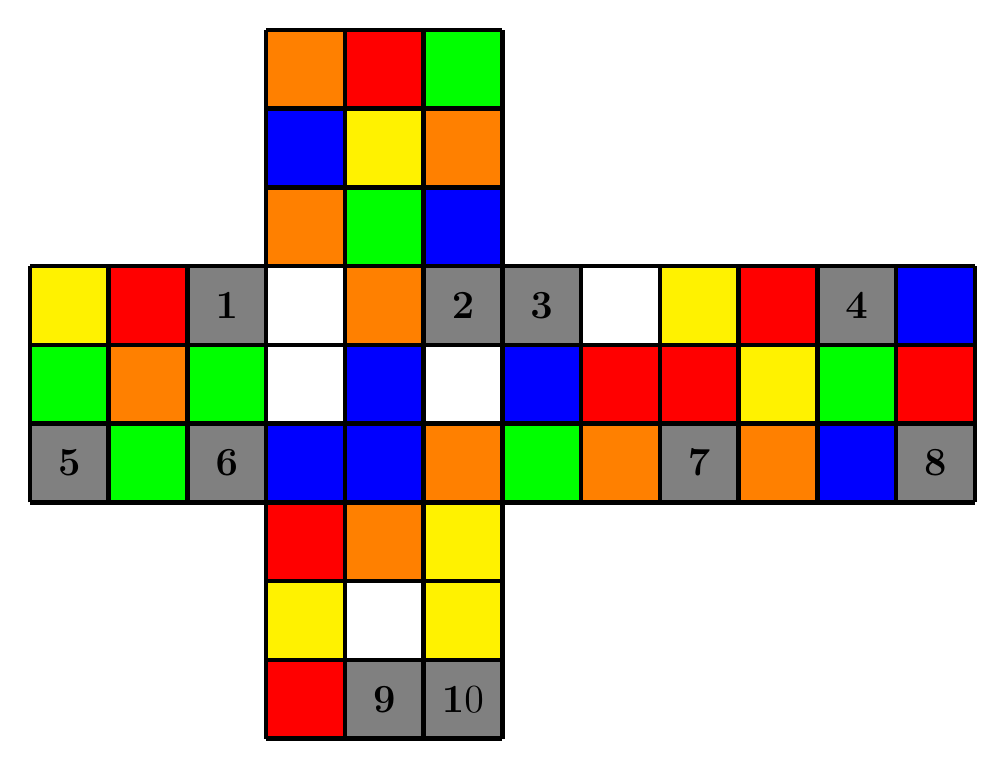
\begin{tikzpicture}[every node/.style={minimum size=1cm-\pgflinewidth, outer sep=0pt}]
\node[fill=orange] at (0.5,5.5) {};
\node[fill=red] at (1.5,5.5) {};
\node[fill=green] at (2.5,5.5) {};
\node[fill=blue] at (0.5,4.5) {};
\node[fill=yellow] at (1.5,4.5) {};
\node[fill=orange] at (2.5,4.5) {};
\node[fill=orange] at (0.5,3.5) {};
\node[fill=green] at (1.5,3.5) {};
\node[fill=blue] at (2.5,3.5) {};

\node[fill=yellow] at (-2.5,2.5) {};
\node[fill=red] at (-1.5,2.5) {};
\node[fill=gray] at (-0.5,2.5) {\Large \textbf 1};
\node[fill=white] at (0.5,2.5) {};
\node[fill=orange] at (1.5,2.5) {};
\node[fill=gray] at (2.5,2.5) {\Large \textbf 2};
\node[fill=gray] at (3.5,2.5) {\Large \textbf 3};
\node[fill=white] at (4.5,2.5) {};
\node[fill=yellow] at (5.5,2.5) {};
\node[fill=red] at (6.5,2.5) {};
\node[fill=gray] at (7.5,2.5) {\Large \textbf 4};
\node[fill=blue] at (8.5,2.5) {};

\node[fill=green] at (-2.5,1.5) {};
\node[fill=orange] at (-1.5,1.5) {};
\node[fill=green] at (-0.5,1.5) {};
\node[fill=white] at (0.5,1.5) {};
\node[fill=blue] at (1.5,1.5) {};
\node[fill=white] at (2.5,1.5) {};
\node[fill=blue] at (3.5,1.5) {};
\node[fill=red] at (4.5,1.5) {};
\node[fill=red] at (5.5,1.5) {};
\node[fill=yellow] at (6.5,1.5) {};
\node[fill=green] at (7.5,1.5) {};
\node[fill=red] at (8.5,1.5) {};

\node[fill=gray] at (-2.5,0.5) {\Large \textbf 5};
\node[fill=green] at (-1.5,0.5) {};
\node[fill=gray] at (-0.5,0.5) {\Large \textbf 6};
\node[fill=blue] at (0.5,0.5) {};
\node[fill=blue] at (1.5,0.5) {};
\node[fill=orange] at (2.5,0.5) {};
\node[fill=green] at (3.5,0.5) {};
\node[fill=orange] at (4.5,0.5) {};
\node[fill=gray] at (5.5,0.5) {\Large \textbf 7};
\node[fill=orange] at (6.5,0.5) {};
\node[fill=blue] at (7.5,0.5) {};
\node[fill=gray] at (8.5,0.5) {\Large \textbf 8};

\node[fill=red] at (0.5,-0.5) {};
\node[fill=orange] at (1.5,-0.5) {};
\node[fill=yellow] at (2.5,-0.5) {};
\node[fill=yellow] at (0.5,-1.5) {};
\node[fill=white] at (1.5,-1.5) {};
\node[fill=yellow] at (2.5,-1.5) {};
\node[fill=red] at (0.5,-2.5) {};
\node[fill=gray] at (1.5,-2.5) {\Large \textbf 9};
\node[fill=gray] at (2.5,-2.5) {\Large \textbf 10};

\draw[step=1cm,color=black, ultra thick] (-3,0) grid (9,3);
\draw[step=1cm,color=black, ultra thick] (0,-3) grid (3,0);
\draw[step=1cm,color=black, ultra thick] (0,3) grid (3,6);
\end{tikzpicture}
\vspace{0.1cm}
\\
\noindent\normalsize \newtime  \textbf{Solution 46: U R F U' B2 D2 L F2 R2 U F' L B2 F R2 U' R F' L' D' Uw' }
\vspace{1cm}



{\noindent\Large  \newtime \textbf{No. 47\qquad Difficulty: $\bigstar\bigstar$}}
\vspace{0.2cm}\\
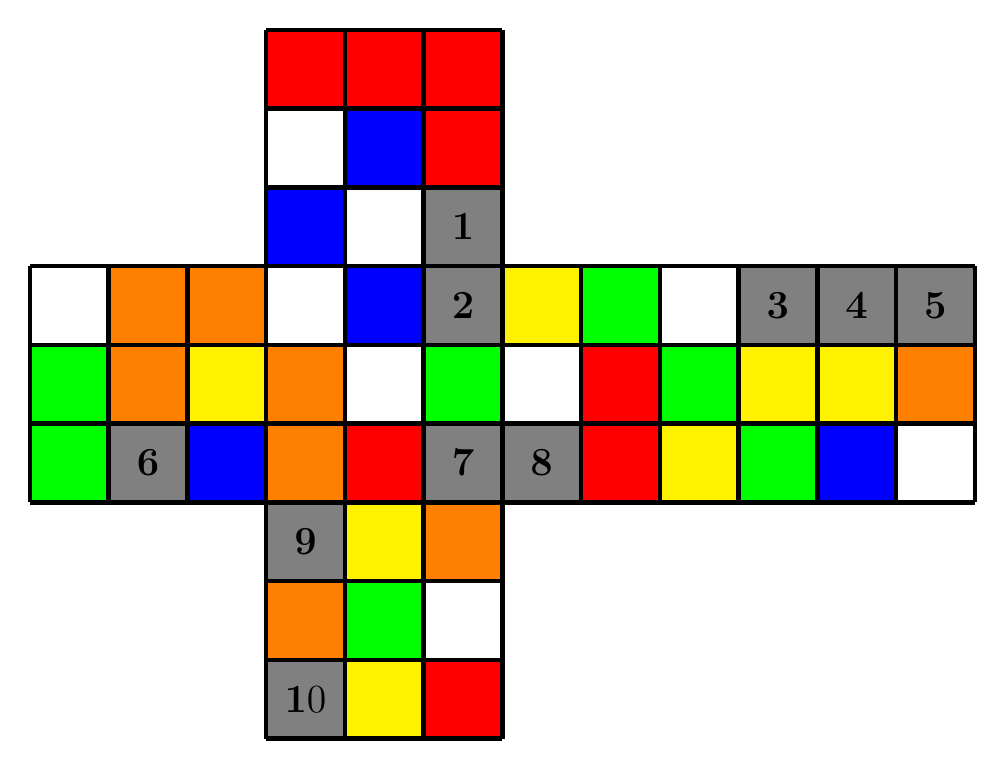
\begin{tikzpicture}[every node/.style={minimum size=1cm-\pgflinewidth, outer sep=0pt}]
\node[fill=red] at (0.5,5.5) {};
\node[fill=red] at (1.5,5.5) {};
\node[fill=red] at (2.5,5.5) {};
\node[fill=white] at (0.5,4.5) {};
\node[fill=blue] at (1.5,4.5) {};
\node[fill=red] at (2.5,4.5) {};
\node[fill=blue] at (0.5,3.5) {};
\node[fill=white] at (1.5,3.5) {};
\node[fill=gray] at (2.5,3.5) {\Large \textbf 1};

\node[fill=white] at (-2.5,2.5) {};
\node[fill=orange] at (-1.5,2.5) {};
\node[fill=orange] at (-0.5,2.5) {};
\node[fill=white] at (0.5,2.5) {};
\node[fill=blue] at (1.5,2.5) {};
\node[fill=gray] at (2.5,2.5) {\Large \textbf 2};
\node[fill=yellow] at (3.5,2.5) {};
\node[fill=green] at (4.5,2.5) {};
\node[fill=white] at (5.5,2.5) {};
\node[fill=gray] at (6.5,2.5) {\Large \textbf 3};
\node[fill=gray] at (7.5,2.5) {\Large \textbf 4};
\node[fill=gray] at (8.5,2.5) {\Large \textbf 5};

\node[fill=green] at (-2.5,1.5) {};
\node[fill=orange] at (-1.5,1.5) {};
\node[fill=yellow] at (-0.5,1.5) {};
\node[fill=orange] at (0.5,1.5) {};
\node[fill=white] at (1.5,1.5) {};
\node[fill=green] at (2.5,1.5) {};
\node[fill=white] at (3.5,1.5) {};
\node[fill=red] at (4.5,1.5) {};
\node[fill=green] at (5.5,1.5) {};
\node[fill=yellow] at (6.5,1.5) {};
\node[fill=yellow] at (7.5,1.5) {};
\node[fill=orange] at (8.5,1.5) {};

\node[fill=green] at (-2.5,0.5) {};
\node[fill=gray] at (-1.5,0.5) {\Large \textbf 6};
\node[fill=blue] at (-0.5,0.5) {};
\node[fill=orange] at (0.5,0.5) {};
\node[fill=red] at (1.5,0.5) {};
\node[fill=gray] at (2.5,0.5) {\Large \textbf 7};
\node[fill=gray] at (3.5,0.5) {\Large \textbf 8};
\node[fill=red] at (4.5,0.5) {};
\node[fill=yellow] at (5.5,0.5) {};
\node[fill=green] at (6.5,0.5) {};
\node[fill=blue] at (7.5,0.5) {};
\node[fill=white] at (8.5,0.5) {};

\node[fill=gray] at (0.5,-0.5) {\Large \textbf 9};
\node[fill=yellow] at (1.5,-0.5) {};
\node[fill=orange] at (2.5,-0.5) {};
\node[fill=orange] at (0.5,-1.5) {};
\node[fill=green] at (1.5,-1.5) {};
\node[fill=white] at (2.5,-1.5) {};
\node[fill=gray] at (0.5,-2.5) {\Large \textbf 10};
\node[fill=yellow] at (1.5,-2.5) {};
\node[fill=red] at (2.5,-2.5) {};

\draw[step=1cm,color=black, ultra thick] (-3,0) grid (9,3);
\draw[step=1cm,color=black, ultra thick] (0,-3) grid (3,0);
\draw[step=1cm,color=black, ultra thick] (0,3) grid (3,6);
\end{tikzpicture}
\vspace{0.1cm}
\\
\noindent\normalsize \newtime  \textbf{Solution 47: L2 D2 L2 B' F D F' L B D2 U2 R2 B' U R2 B' R2 F' R2 L' Fw Uw' }
\vspace{1cm}



{\noindent\Large  \newtime \textbf{No. 48\qquad Difficulty: $\bigstar\bigstar$}}
\vspace{0.2cm}\\
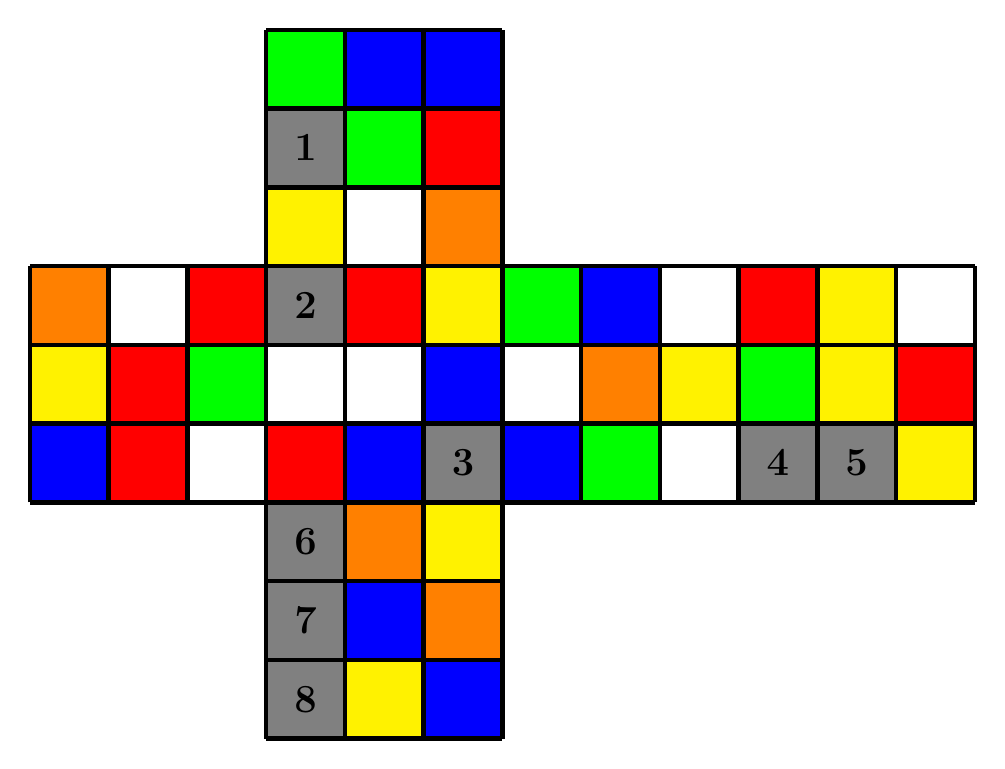
\begin{tikzpicture}[every node/.style={minimum size=1cm-\pgflinewidth, outer sep=0pt}]
\node[fill=green] at (0.5,5.5) {};
\node[fill=blue] at (1.5,5.5) {};
\node[fill=blue] at (2.5,5.5) {};
\node[fill=gray] at (0.5,4.5) {\Large \textbf 1};
\node[fill=green] at (1.5,4.5) {};
\node[fill=red] at (2.5,4.5) {};
\node[fill=yellow] at (0.5,3.5) {};
\node[fill=white] at (1.5,3.5) {};
\node[fill=orange] at (2.5,3.5) {};

\node[fill=orange] at (-2.5,2.5) {};
\node[fill=white] at (-1.5,2.5) {};
\node[fill=red] at (-0.5,2.5) {};
\node[fill=gray] at (0.5,2.5) {\Large \textbf 2};
\node[fill=red] at (1.5,2.5) {};
\node[fill=yellow] at (2.5,2.5) {};
\node[fill=green] at (3.5,2.5) {};
\node[fill=blue] at (4.5,2.5) {};
\node[fill=white] at (5.5,2.5) {};
\node[fill=red] at (6.5,2.5) {};
\node[fill=yellow] at (7.5,2.5) {};
\node[fill=white] at (8.5,2.5) {};

\node[fill=yellow] at (-2.5,1.5) {};
\node[fill=red] at (-1.5,1.5) {};
\node[fill=green] at (-0.5,1.5) {};
\node[fill=white] at (0.5,1.5) {};
\node[fill=white] at (1.5,1.5) {};
\node[fill=blue] at (2.5,1.5) {};
\node[fill=white] at (3.5,1.5) {};
\node[fill=orange] at (4.5,1.5) {};
\node[fill=yellow] at (5.5,1.5) {};
\node[fill=green] at (6.5,1.5) {};
\node[fill=yellow] at (7.5,1.5) {};
\node[fill=red] at (8.5,1.5) {};

\node[fill=blue] at (-2.5,0.5) {};
\node[fill=red] at (-1.5,0.5) {};
\node[fill=white] at (-0.5,0.5) {};
\node[fill=red] at (0.5,0.5) {};
\node[fill=blue] at (1.5,0.5) {};
\node[fill=gray] at (2.5,0.5) {\Large \textbf 3};
\node[fill=blue] at (3.5,0.5) {};
\node[fill=green] at (4.5,0.5) {};
\node[fill=white] at (5.5,0.5) {};
\node[fill=gray] at (6.5,0.5) {\Large \textbf 4};
\node[fill=gray] at (7.5,0.5) {\Large \textbf 5};
\node[fill=yellow] at (8.5,0.5) {};

\node[fill=gray] at (0.5,-0.5) {\Large \textbf 6};
\node[fill=orange] at (1.5,-0.5) {};
\node[fill=yellow] at (2.5,-0.5) {};
\node[fill=gray] at (0.5,-1.5) {\Large \textbf 7};
\node[fill=blue] at (1.5,-1.5) {};
\node[fill=orange] at (2.5,-1.5) {};
\node[fill=gray] at (0.5,-2.5) {\Large \textbf 8};
\node[fill=yellow] at (1.5,-2.5) {};
\node[fill=blue] at (2.5,-2.5) {};

\draw[step=1cm,color=black, ultra thick] (-3,0) grid (9,3);
\draw[step=1cm,color=black, ultra thick] (0,-3) grid (3,0);
\draw[step=1cm,color=black, ultra thick] (0,3) grid (3,6);
\end{tikzpicture}
\vspace{0.1cm}
\\
\noindent\normalsize \newtime  \textbf{Solution 48: L B2 R B' F' U L2 R' F R F U2 L' F2 B2 L2 B F U' R' Fw' Uw }
\vspace{1cm}



{\noindent\Large  \newtime \textbf{No. 49\qquad Difficulty: $\bigstar\bigstar$}}
\vspace{0.2cm}\\
\begin{tikzpicture}[every node/.style={minimum size=1cm-\pgflinewidth, outer sep=0pt}]
\node[fill=yellow] at (0.5,5.5) {};
\node[fill=gray] at (1.5,5.5) {\Large \textbf 1};
\node[fill=yellow] at (2.5,5.5) {};
\node[fill=white] at (0.5,4.5) {};
\node[fill=green] at (1.5,4.5) {};
\node[fill=white] at (2.5,4.5) {};
\node[fill=gray] at (0.5,3.5) {\Large \textbf 2};
\node[fill=orange] at (1.5,3.5) {};
\node[fill=gray] at (2.5,3.5) {\Large \textbf 3};

\node[fill=orange] at (-2.5,2.5) {};
\node[fill=gray] at (-1.5,2.5) {\Large \textbf 4};
\node[fill=red] at (-0.5,2.5) {};
\node[fill=white] at (0.5,2.5) {};
\node[fill=gray] at (1.5,2.5) {\Large \textbf 5};
\node[fill=orange] at (2.5,2.5) {};
\node[fill=gray] at (3.5,2.5) {\Large \textbf 6};
\node[fill=blue] at (4.5,2.5) {};
\node[fill=blue] at (5.5,2.5) {};
\node[fill=red] at (6.5,2.5) {};
\node[fill=yellow] at (7.5,2.5) {};
\node[fill=green] at (8.5,2.5) {};

\node[fill=green] at (-2.5,1.5) {};
\node[fill=red] at (-1.5,1.5) {};
\node[fill=yellow] at (-0.5,1.5) {};
\node[fill=orange] at (0.5,1.5) {};
\node[fill=white] at (1.5,1.5) {};
\node[fill=yellow] at (2.5,1.5) {};
\node[fill=red] at (3.5,1.5) {};
\node[fill=orange] at (4.5,1.5) {};
\node[fill=green] at (5.5,1.5) {};
\node[fill=orange] at (6.5,1.5) {};
\node[fill=yellow] at (7.5,1.5) {};
\node[fill=gray] at (8.5,1.5) {\Large \textbf 7};

\node[fill=blue] at (-2.5,0.5) {};
\node[fill=blue] at (-1.5,0.5) {};
\node[fill=gray] at (-0.5,0.5) {\Large \textbf 8};
\node[fill=green] at (0.5,0.5) {};
\node[fill=red] at (1.5,0.5) {};
\node[fill=gray] at (2.5,0.5) {\Large \textbf 9};
\node[fill=red] at (3.5,0.5) {};
\node[fill=blue] at (4.5,0.5) {};
\node[fill=red] at (5.5,0.5) {};
\node[fill=white] at (6.5,0.5) {};
\node[fill=green] at (7.5,0.5) {};
\node[fill=gray] at (8.5,0.5) {\Large \textbf 10};

\node[fill=orange] at (0.5,-0.5) {};
\node[fill=green] at (1.5,-0.5) {};
\node[fill=yellow] at (2.5,-0.5) {};
\node[fill=orange] at (0.5,-1.5) {};
\node[fill=blue] at (1.5,-1.5) {};
\node[fill=red] at (2.5,-1.5) {};
\node[fill=gray] at (0.5,-2.5) {\Large \textbf 11};
\node[fill=yellow] at (1.5,-2.5) {};
\node[fill=gray] at (2.5,-2.5) {\Large \textbf 12};

\draw[step=1cm,color=black, ultra thick] (-3,0) grid (9,3);
\draw[step=1cm,color=black, ultra thick] (0,-3) grid (3,0);
\draw[step=1cm,color=black, ultra thick] (0,3) grid (3,6);
\end{tikzpicture}
\vspace{0.1cm}
\\
\noindent\normalsize \newtime  \textbf{Solution 49: F R2 L2 U B' U F U' B' L R' U D' R2 B2 D' U' R' D L Fw' Uw }
\vspace{1cm}



{\noindent\Large  \newtime \textbf{No. 50\qquad Difficulty: $\bigstar\bigstar$}}
\vspace{0.2cm}\\
\begin{tikzpicture}[every node/.style={minimum size=1cm-\pgflinewidth, outer sep=0pt}]
\node[fill=blue] at (0.5,5.5) {};
\node[fill=gray] at (1.5,5.5) {\Large \textbf 1};
\node[fill=red] at (2.5,5.5) {};
\node[fill=yellow] at (0.5,4.5) {};
\node[fill=orange] at (1.5,4.5) {};
\node[fill=red] at (2.5,4.5) {};
\node[fill=gray] at (0.5,3.5) {\Large \textbf 2};
\node[fill=green] at (1.5,3.5) {};
\node[fill=orange] at (2.5,3.5) {};

\node[fill=gray] at (-2.5,2.5) {\Large \textbf 3};
\node[fill=green] at (-1.5,2.5) {};
\node[fill=white] at (-0.5,2.5) {};
\node[fill=orange] at (0.5,2.5) {};
\node[fill=gray] at (1.5,2.5) {\Large \textbf 4};
\node[fill=blue] at (2.5,2.5) {};
\node[fill=yellow] at (3.5,2.5) {};
\node[fill=white] at (4.5,2.5) {};
\node[fill=blue] at (5.5,2.5) {};
\node[fill=white] at (6.5,2.5) {};
\node[fill=yellow] at (7.5,2.5) {};
\node[fill=gray] at (8.5,2.5) {\Large \textbf 5};

\node[fill=white] at (-2.5,1.5) {};
\node[fill=white] at (-1.5,1.5) {};
\node[fill=orange] at (-0.5,1.5) {};
\node[fill=blue] at (0.5,1.5) {};
\node[fill=blue] at (1.5,1.5) {};
\node[fill=orange] at (2.5,1.5) {};
\node[fill=white] at (3.5,1.5) {};
\node[fill=yellow] at (4.5,1.5) {};
\node[fill=blue] at (5.5,1.5) {};
\node[fill=white] at (6.5,1.5) {};
\node[fill=green] at (7.5,1.5) {};
\node[fill=gray] at (8.5,1.5) {\Large \textbf 6};

\node[fill=yellow] at (-2.5,0.5) {};
\node[fill=yellow] at (-1.5,0.5) {};
\node[fill=blue] at (-0.5,0.5) {};
\node[fill=white] at (0.5,0.5) {};
\node[fill=red] at (1.5,0.5) {};
\node[fill=gray] at (2.5,0.5) {\Large \textbf 7};
\node[fill=green] at (3.5,0.5) {};
\node[fill=blue] at (4.5,0.5) {};
\node[fill=green] at (5.5,0.5) {};
\node[fill=white] at (6.5,0.5) {};
\node[fill=red] at (7.5,0.5) {};
\node[fill=gray] at (8.5,0.5) {\Large \textbf 8};

\node[fill=gray] at (0.5,-0.5) {\Large \textbf 9};
\node[fill=green] at (1.5,-0.5) {};
\node[fill=gray] at (2.5,-0.5) {\Large \textbf 10};
\node[fill=orange] at (0.5,-1.5) {};
\node[fill=red] at (1.5,-1.5) {};
\node[fill=gray] at (2.5,-1.5) {\Large \textbf 11};
\node[fill=orange] at (0.5,-2.5) {};
\node[fill=yellow] at (1.5,-2.5) {};
\node[fill=gray] at (2.5,-2.5) {\Large \textbf 12};

\draw[step=1cm,color=black, ultra thick] (-3,0) grid (9,3);
\draw[step=1cm,color=black, ultra thick] (0,-3) grid (3,0);
\draw[step=1cm,color=black, ultra thick] (0,3) grid (3,6);
\end{tikzpicture}
\vspace{0.1cm}
\\
\noindent\normalsize \newtime  \textbf{Solution 50: U D L F B2 R2 B2 L' D2 L B' L D F2 D' B2 R2 D U' B2 Rw' Uw' }
\vspace{1cm}



{\noindent\Large  \newtime \textbf{No. 51\qquad Difficulty: $\bigstar\bigstar\bigstar$}}
\vspace{0.2cm}\\
\begin{tikzpicture}[every node/.style={minimum size=1cm-\pgflinewidth, outer sep=0pt}]
\node[fill=red] at (0.5,5.5) {};
\node[fill=red] at (1.5,5.5) {};
\node[fill=yellow] at (2.5,5.5) {};
\node[fill=white] at (0.5,4.5) {};
\node[fill=orange] at (1.5,4.5) {};
\node[fill=green] at (2.5,4.5) {};
\node[fill=gray] at (0.5,3.5) {\Large \textbf 1};
\node[fill=blue] at (1.5,3.5) {};
\node[fill=blue] at (2.5,3.5) {};

\node[fill=white] at (-2.5,2.5) {};
\node[fill=red] at (-1.5,2.5) {};
\node[fill=blue] at (-0.5,2.5) {};
\node[fill=gray] at (0.5,2.5) {\Large \textbf 2};
\node[fill=gray] at (1.5,2.5) {\Large \textbf 3};
\node[fill=yellow] at (2.5,2.5) {};
\node[fill=gray] at (3.5,2.5) {\Large \textbf 4};
\node[fill=orange] at (4.5,2.5) {};
\node[fill=red] at (5.5,2.5) {};
\node[fill=green] at (6.5,2.5) {};
\node[fill=green] at (7.5,2.5) {};
\node[fill=gray] at (8.5,2.5) {\Large \textbf 5};

\node[fill=blue] at (-2.5,1.5) {};
\node[fill=green] at (-1.5,1.5) {};
\node[fill=green] at (-0.5,1.5) {};
\node[fill=yellow] at (0.5,1.5) {};
\node[fill=white] at (1.5,1.5) {};
\node[fill=blue] at (2.5,1.5) {};
\node[fill=red] at (3.5,1.5) {};
\node[fill=blue] at (4.5,1.5) {};
\node[fill=gray] at (5.5,1.5) {\Large \textbf 6};
\node[fill=orange] at (6.5,1.5) {};
\node[fill=yellow] at (7.5,1.5) {};
\node[fill=orange] at (8.5,1.5) {};

\node[fill=white] at (-2.5,0.5) {};
\node[fill=yellow] at (-1.5,0.5) {};
\node[fill=gray] at (-0.5,0.5) {\Large \textbf 7};
\node[fill=white] at (0.5,0.5) {};
\node[fill=yellow] at (1.5,0.5) {};
\node[fill=orange] at (2.5,0.5) {};
\node[fill=gray] at (3.5,0.5) {\Large \textbf 8};
\node[fill=blue] at (4.5,0.5) {};
\node[fill=gray] at (5.5,0.5) {\Large \textbf 9};
\node[fill=white] at (6.5,0.5) {};
\node[fill=green] at (7.5,0.5) {};
\node[fill=green] at (8.5,0.5) {};

\node[fill=green] at (0.5,-0.5) {};
\node[fill=gray] at (1.5,-0.5) {\Large \textbf 10};
\node[fill=yellow] at (2.5,-0.5) {};
\node[fill=orange] at (0.5,-1.5) {};
\node[fill=red] at (1.5,-1.5) {};
\node[fill=white] at (2.5,-1.5) {};
\node[fill=gray] at (0.5,-2.5) {\Large \textbf 11};
\node[fill=white] at (1.5,-2.5) {};
\node[fill=orange] at (2.5,-2.5) {};

\draw[step=1cm,color=black, ultra thick] (-3,0) grid (9,3);
\draw[step=1cm,color=black, ultra thick] (0,-3) grid (3,0);
\draw[step=1cm,color=black, ultra thick] (0,3) grid (3,6);
\end{tikzpicture}
\vspace{0.1cm}
\\
\noindent\normalsize \newtime  \textbf{Solution 51: R' D2 F' D F2 L F' B L' F2 L U L' U2 B U' D2 L D2 F2 Rw' Uw2 }
\vspace{1cm}



{\noindent\Large  \newtime \textbf{No. 52\qquad Difficulty: $\bigstar\bigstar\bigstar$}}
\vspace{0.2cm}\\
\begin{tikzpicture}[every node/.style={minimum size=1cm-\pgflinewidth, outer sep=0pt}]
\node[fill=gray] at (0.5,5.5) {\Large \textbf 1};
\node[fill=orange] at (1.5,5.5) {};
\node[fill=gray] at (2.5,5.5) {\Large \textbf 2};
\node[fill=yellow] at (0.5,4.5) {};
\node[fill=green] at (1.5,4.5) {};
\node[fill=orange] at (2.5,4.5) {};
\node[fill=red] at (0.5,3.5) {};
\node[fill=gray] at (1.5,3.5) {\Large \textbf 3};
\node[fill=blue] at (2.5,3.5) {};

\node[fill=orange] at (-2.5,2.5) {};
\node[fill=orange] at (-1.5,2.5) {};
\node[fill=gray] at (-0.5,2.5) {\Large \textbf 4};
\node[fill=green] at (0.5,2.5) {};
\node[fill=blue] at (1.5,2.5) {};
\node[fill=gray] at (2.5,2.5) {\Large \textbf 5};
\node[fill=yellow] at (3.5,2.5) {};
\node[fill=gray] at (4.5,2.5) {\Large \textbf 6};
\node[fill=gray] at (5.5,2.5) {\Large \textbf 7};
\node[fill=blue] at (6.5,2.5) {};
\node[fill=green] at (7.5,2.5) {};
\node[fill=yellow] at (8.5,2.5) {};

\node[fill=white] at (-2.5,1.5) {};
\node[fill=white] at (-1.5,1.5) {};
\node[fill=green] at (-0.5,1.5) {};
\node[fill=white] at (0.5,1.5) {};
\node[fill=orange] at (1.5,1.5) {};
\node[fill=orange] at (2.5,1.5) {};
\node[fill=white] at (3.5,1.5) {};
\node[fill=yellow] at (4.5,1.5) {};
\node[fill=blue] at (5.5,1.5) {};
\node[fill=red] at (6.5,1.5) {};
\node[fill=red] at (7.5,1.5) {};
\node[fill=red] at (8.5,1.5) {};

\node[fill=green] at (-2.5,0.5) {};
\node[fill=yellow] at (-1.5,0.5) {};
\node[fill=gray] at (-0.5,0.5) {\Large \textbf 8};
\node[fill=gray] at (0.5,0.5) {\Large \textbf 9};
\node[fill=gray] at (1.5,0.5) {\Large \textbf 10};
\node[fill=white] at (2.5,0.5) {};
\node[fill=blue] at (3.5,0.5) {};
\node[fill=gray] at (4.5,0.5) {\Large \textbf 11};
\node[fill=red] at (5.5,0.5) {};
\node[fill=yellow] at (6.5,0.5) {};
\node[fill=yellow] at (7.5,0.5) {};
\node[fill=orange] at (8.5,0.5) {};

\node[fill=gray] at (0.5,-0.5) {\Large \textbf 12};
\node[fill=yellow] at (1.5,-0.5) {};
\node[fill=red] at (2.5,-0.5) {};
\node[fill=green] at (0.5,-1.5) {};
\node[fill=blue] at (1.5,-1.5) {};
\node[fill=red] at (2.5,-1.5) {};
\node[fill=gray] at (0.5,-2.5) {\Large \textbf 13};
\node[fill=blue] at (1.5,-2.5) {};
\node[fill=gray] at (2.5,-2.5) {\Large \textbf 14};

\draw[step=1cm,color=black, ultra thick] (-3,0) grid (9,3);
\draw[step=1cm,color=black, ultra thick] (0,-3) grid (3,0);
\draw[step=1cm,color=black, ultra thick] (0,3) grid (3,6);
\end{tikzpicture}
\vspace{0.1cm}
\\
\noindent\normalsize \newtime  \textbf{Solution 52: D2 R' L' B2 L' U2 D' R' U' B' L R2 F U D' L U R B R' Fw' Uw2 }
\vspace{1cm}



{\noindent\Large  \newtime \textbf{No. 53\qquad Difficulty: $\bigstar\bigstar\bigstar$}}
\vspace{0.2cm}\\
\begin{tikzpicture}[every node/.style={minimum size=1cm-\pgflinewidth, outer sep=0pt}]
\node[fill=blue] at (0.5,5.5) {};
\node[fill=red] at (1.5,5.5) {};
\node[fill=gray] at (2.5,5.5) {\Large \textbf 1};
\node[fill=white] at (0.5,4.5) {};
\node[fill=blue] at (1.5,4.5) {};
\node[fill=blue] at (2.5,4.5) {};
\node[fill=white] at (0.5,3.5) {};
\node[fill=green] at (1.5,3.5) {};
\node[fill=white] at (2.5,3.5) {};

\node[fill=orange] at (-2.5,2.5) {};
\node[fill=gray] at (-1.5,2.5) {\Large \textbf 2};
\node[fill=blue] at (-0.5,2.5) {};
\node[fill=orange] at (0.5,2.5) {};
\node[fill=orange] at (1.5,2.5) {};
\node[fill=gray] at (2.5,2.5) {\Large \textbf 3};
\node[fill=red] at (3.5,2.5) {};
\node[fill=yellow] at (4.5,2.5) {};
\node[fill=gray] at (5.5,2.5) {\Large \textbf 4};
\node[fill=gray] at (6.5,2.5) {\Large \textbf 5};
\node[fill=gray] at (7.5,2.5) {\Large \textbf 6};
\node[fill=gray] at (8.5,2.5) {\Large \textbf 7};

\node[fill=green] at (-2.5,1.5) {};
\node[fill=orange] at (-1.5,1.5) {};
\node[fill=yellow] at (-0.5,1.5) {};
\node[fill=red] at (0.5,1.5) {};
\node[fill=white] at (1.5,1.5) {};
\node[fill=gray] at (2.5,1.5) {\Large \textbf 8};
\node[fill=yellow] at (3.5,1.5) {};
\node[fill=red] at (4.5,1.5) {};
\node[fill=red] at (5.5,1.5) {};
\node[fill=blue] at (6.5,1.5) {};
\node[fill=yellow] at (7.5,1.5) {};
\node[fill=white] at (8.5,1.5) {};

\node[fill=gray] at (-2.5,0.5) {\Large \textbf 9};
\node[fill=orange] at (-1.5,0.5) {};
\node[fill=red] at (-0.5,0.5) {};
\node[fill=white] at (0.5,0.5) {};
\node[fill=gray] at (1.5,0.5) {\Large \textbf 10};
\node[fill=red] at (2.5,0.5) {};
\node[fill=blue] at (3.5,0.5) {};
\node[fill=red] at (4.5,0.5) {};
\node[fill=green] at (5.5,0.5) {};
\node[fill=orange] at (6.5,0.5) {};
\node[fill=blue] at (7.5,0.5) {};
\node[fill=green] at (8.5,0.5) {};

\node[fill=gray] at (0.5,-0.5) {\Large \textbf 11};
\node[fill=green] at (1.5,-0.5) {};
\node[fill=gray] at (2.5,-0.5) {\Large \textbf 12};
\node[fill=white] at (0.5,-1.5) {};
\node[fill=green] at (1.5,-1.5) {};
\node[fill=green] at (2.5,-1.5) {};
\node[fill=orange] at (0.5,-2.5) {};
\node[fill=gray] at (1.5,-2.5) {\Large \textbf 13};
\node[fill=gray] at (2.5,-2.5) {\Large \textbf 14};

\draw[step=1cm,color=black, ultra thick] (-3,0) grid (9,3);
\draw[step=1cm,color=black, ultra thick] (0,-3) grid (3,0);
\draw[step=1cm,color=black, ultra thick] (0,3) grid (3,6);
\end{tikzpicture}
\vspace{0.1cm}
\\
\noindent\normalsize \newtime  \textbf{Solution 53: F' L2 F L R2 U R' U' D2 B' U' B' D2 B F2 D2 R B' U' F' Fw Uw' }
\vspace{1cm}



{\noindent\Large  \newtime \textbf{No. 54\qquad Difficulty: $\bigstar\bigstar\bigstar$}}
\vspace{0.2cm}\\
\begin{tikzpicture}[every node/.style={minimum size=1cm-\pgflinewidth, outer sep=0pt}]
\node[fill=gray] at (0.5,5.5) {\Large \textbf 1};
\node[fill=yellow] at (1.5,5.5) {};
\node[fill=gray] at (2.5,5.5) {\Large \textbf 2};
\node[fill=gray] at (0.5,4.5) {\Large \textbf 3};
\node[fill=green] at (1.5,4.5) {};
\node[fill=gray] at (2.5,4.5) {\Large \textbf 4};
\node[fill=orange] at (0.5,3.5) {};
\node[fill=red] at (1.5,3.5) {};
\node[fill=gray] at (2.5,3.5) {\Large \textbf 5};

\node[fill=gray] at (-2.5,2.5) {\Large \textbf 6};
\node[fill=white] at (-1.5,2.5) {};
\node[fill=gray] at (-0.5,2.5) {\Large \textbf 7};
\node[fill=yellow] at (0.5,2.5) {};
\node[fill=green] at (1.5,2.5) {};
\node[fill=green] at (2.5,2.5) {};
\node[fill=gray] at (3.5,2.5) {\Large \textbf 8};
\node[fill=orange] at (4.5,2.5) {};
\node[fill=white] at (5.5,2.5) {};
\node[fill=gray] at (6.5,2.5) {\Large \textbf 9};
\node[fill=green] at (7.5,2.5) {};
\node[fill=red] at (8.5,2.5) {};

\node[fill=blue] at (-2.5,1.5) {};
\node[fill=orange] at (-1.5,1.5) {};
\node[fill=white] at (-0.5,1.5) {};
\node[fill=red] at (0.5,1.5) {};
\node[fill=yellow] at (1.5,1.5) {};
\node[fill=white] at (2.5,1.5) {};
\node[fill=orange] at (3.5,1.5) {};
\node[fill=red] at (4.5,1.5) {};
\node[fill=green] at (5.5,1.5) {};
\node[fill=white] at (6.5,1.5) {};
\node[fill=white] at (7.5,1.5) {};
\node[fill=yellow] at (8.5,1.5) {};

\node[fill=red] at (-2.5,0.5) {};
\node[fill=orange] at (-1.5,0.5) {};
\node[fill=white] at (-0.5,0.5) {};
\node[fill=gray] at (0.5,0.5) {\Large \textbf 10};
\node[fill=yellow] at (1.5,0.5) {};
\node[fill=red] at (2.5,0.5) {};
\node[fill=green] at (3.5,0.5) {};
\node[fill=gray] at (4.5,0.5) {\Large \textbf 11};
\node[fill=white] at (5.5,0.5) {};
\node[fill=blue] at (6.5,0.5) {};
\node[fill=red] at (7.5,0.5) {};
\node[fill=green] at (8.5,0.5) {};

\node[fill=blue] at (0.5,-0.5) {};
\node[fill=gray] at (1.5,-0.5) {\Large \textbf 12};
\node[fill=gray] at (2.5,-0.5) {\Large \textbf 13};
\node[fill=yellow] at (0.5,-1.5) {};
\node[fill=blue] at (1.5,-1.5) {};
\node[fill=green] at (2.5,-1.5) {};
\node[fill=yellow] at (0.5,-2.5) {};
\node[fill=blue] at (1.5,-2.5) {};
\node[fill=red] at (2.5,-2.5) {};

\draw[step=1cm,color=black, ultra thick] (-3,0) grid (9,3);
\draw[step=1cm,color=black, ultra thick] (0,-3) grid (3,0);
\draw[step=1cm,color=black, ultra thick] (0,3) grid (3,6);
\end{tikzpicture}
\vspace{0.1cm}
\\
\noindent\normalsize \newtime  \textbf{Solution 54: D2 F' U2 F' B' R D2 U' R' L D U' R B' L D F' D2 U L2 Fw' Uw' }
\vspace{1cm}



{\noindent\Large  \newtime \textbf{No. 55\qquad Difficulty: $\bigstar\bigstar\bigstar$}}
\vspace{0.2cm}\\
\begin{tikzpicture}[every node/.style={minimum size=1cm-\pgflinewidth, outer sep=0pt}]
\node[fill=blue] at (0.5,5.5) {};
\node[fill=blue] at (1.5,5.5) {};
\node[fill=gray] at (2.5,5.5) {\Large \textbf 1};
\node[fill=green] at (0.5,4.5) {};
\node[fill=orange] at (1.5,4.5) {};
\node[fill=yellow] at (2.5,4.5) {};
\node[fill=gray] at (0.5,3.5) {\Large \textbf 2};
\node[fill=red] at (1.5,3.5) {};
\node[fill=green] at (2.5,3.5) {};

\node[fill=gray] at (-2.5,2.5) {\Large \textbf 3};
\node[fill=yellow] at (-1.5,2.5) {};
\node[fill=gray] at (-0.5,2.5) {\Large \textbf 4};
\node[fill=gray] at (0.5,2.5) {\Large \textbf 5};
\node[fill=green] at (1.5,2.5) {};
\node[fill=gray] at (2.5,2.5) {\Large \textbf 6};
\node[fill=white] at (3.5,2.5) {};
\node[fill=gray] at (4.5,2.5) {\Large \textbf 7};
\node[fill=red] at (5.5,2.5) {};
\node[fill=yellow] at (6.5,2.5) {};
\node[fill=white] at (7.5,2.5) {};
\node[fill=gray] at (8.5,2.5) {\Large \textbf 8};

\node[fill=orange] at (-2.5,1.5) {};
\node[fill=green] at (-1.5,1.5) {};
\node[fill=orange] at (-0.5,1.5) {};
\node[fill=yellow] at (0.5,1.5) {};
\node[fill=white] at (1.5,1.5) {};
\node[fill=yellow] at (2.5,1.5) {};
\node[fill=red] at (3.5,1.5) {};
\node[fill=blue] at (4.5,1.5) {};
\node[fill=orange] at (5.5,1.5) {};
\node[fill=blue] at (6.5,1.5) {};
\node[fill=yellow] at (7.5,1.5) {};
\node[fill=green] at (8.5,1.5) {};

\node[fill=yellow] at (-2.5,0.5) {};
\node[fill=white] at (-1.5,0.5) {};
\node[fill=orange] at (-0.5,0.5) {};
\node[fill=green] at (0.5,0.5) {};
\node[fill=gray] at (1.5,0.5) {\Large \textbf 9};
\node[fill=yellow] at (2.5,0.5) {};
\node[fill=green] at (3.5,0.5) {};
\node[fill=orange] at (4.5,0.5) {};
\node[fill=white] at (5.5,0.5) {};
\node[fill=orange] at (6.5,0.5) {};
\node[fill=gray] at (7.5,0.5) {\Large \textbf 10};
\node[fill=orange] at (8.5,0.5) {};

\node[fill=gray] at (0.5,-0.5) {\Large \textbf 11};
\node[fill=blue] at (1.5,-0.5) {};
\node[fill=red] at (2.5,-0.5) {};
\node[fill=red] at (0.5,-1.5) {};
\node[fill=red] at (1.5,-1.5) {};
\node[fill=white] at (2.5,-1.5) {};
\node[fill=gray] at (0.5,-2.5) {\Large \textbf 12};
\node[fill=white] at (1.5,-2.5) {};
\node[fill=gray] at (2.5,-2.5) {\Large \textbf 13};

\draw[step=1cm,color=black, ultra thick] (-3,0) grid (9,3);
\draw[step=1cm,color=black, ultra thick] (0,-3) grid (3,0);
\draw[step=1cm,color=black, ultra thick] (0,3) grid (3,6);
\end{tikzpicture}
\vspace{0.1cm}
\\
\noindent\normalsize \newtime  \textbf{Solution 55: D' B F R' F' D' B' U' L' R2 B2 F R2 B R B2 F2 R2 B2 U' Rw' Uw2 }
\vspace{1cm}



{\noindent\Large  \newtime \textbf{No. 56\qquad Difficulty: $\bigstar\bigstar\bigstar$}}
\vspace{0.2cm}\\
\begin{tikzpicture}[every node/.style={minimum size=1cm-\pgflinewidth, outer sep=0pt}]
\node[fill=yellow] at (0.5,5.5) {};
\node[fill=blue] at (1.5,5.5) {};
\node[fill=gray] at (2.5,5.5) {\Large \textbf 1};
\node[fill=gray] at (0.5,4.5) {\Large \textbf 2};
\node[fill=yellow] at (1.5,4.5) {};
\node[fill=green] at (2.5,4.5) {};
\node[fill=gray] at (0.5,3.5) {\Large \textbf 3};
\node[fill=gray] at (1.5,3.5) {\Large \textbf 4};
\node[fill=gray] at (2.5,3.5) {\Large \textbf 5};

\node[fill=gray] at (-2.5,2.5) {\Large \textbf 6};
\node[fill=green] at (-1.5,2.5) {};
\node[fill=blue] at (-0.5,2.5) {};
\node[fill=orange] at (0.5,2.5) {};
\node[fill=yellow] at (1.5,2.5) {};
\node[fill=gray] at (2.5,2.5) {\Large \textbf 7};
\node[fill=white] at (3.5,2.5) {};
\node[fill=orange] at (4.5,2.5) {};
\node[fill=yellow] at (5.5,2.5) {};
\node[fill=gray] at (6.5,2.5) {\Large \textbf 8};
\node[fill=white] at (7.5,2.5) {};
\node[fill=green] at (8.5,2.5) {};

\node[fill=red] at (-2.5,1.5) {};
\node[fill=green] at (-1.5,1.5) {};
\node[fill=red] at (-0.5,1.5) {};
\node[fill=gray] at (0.5,1.5) {\Large \textbf 9};
\node[fill=orange] at (1.5,1.5) {};
\node[fill=orange] at (2.5,1.5) {};
\node[fill=yellow] at (3.5,1.5) {};
\node[fill=blue] at (4.5,1.5) {};
\node[fill=white] at (5.5,1.5) {};
\node[fill=orange] at (6.5,1.5) {};
\node[fill=red] at (7.5,1.5) {};
\node[fill=green] at (8.5,1.5) {};

\node[fill=blue] at (-2.5,0.5) {};
\node[fill=blue] at (-1.5,0.5) {};
\node[fill=orange] at (-0.5,0.5) {};
\node[fill=yellow] at (0.5,0.5) {};
\node[fill=green] at (1.5,0.5) {};
\node[fill=gray] at (2.5,0.5) {\Large \textbf 10};
\node[fill=yellow] at (3.5,0.5) {};
\node[fill=orange] at (4.5,0.5) {};
\node[fill=white] at (5.5,0.5) {};
\node[fill=gray] at (6.5,0.5) {\Large \textbf 11};
\node[fill=red] at (7.5,0.5) {};
\node[fill=gray] at (8.5,0.5) {\Large \textbf 12};

\node[fill=blue] at (0.5,-0.5) {};
\node[fill=white] at (1.5,-0.5) {};
\node[fill=green] at (2.5,-0.5) {};
\node[fill=yellow] at (0.5,-1.5) {};
\node[fill=white] at (1.5,-1.5) {};
\node[fill=blue] at (2.5,-1.5) {};
\node[fill=red] at (0.5,-2.5) {};
\node[fill=blue] at (1.5,-2.5) {};
\node[fill=green] at (2.5,-2.5) {};

\draw[step=1cm,color=black, ultra thick] (-3,0) grid (9,3);
\draw[step=1cm,color=black, ultra thick] (0,-3) grid (3,0);
\draw[step=1cm,color=black, ultra thick] (0,3) grid (3,6);
\end{tikzpicture}
\vspace{0.1cm}
\\
\noindent\normalsize \newtime  \textbf{Solution 56: R' U F R2 D2 U2 R B' U2 B' D' F B' R' U' R F D U F Uw2 }
\vspace{1cm}



{\noindent\Large  \newtime \textbf{No. 57\qquad Difficulty: $\bigstar\bigstar\bigstar$}}
\vspace{0.2cm}\\
\begin{tikzpicture}[every node/.style={minimum size=1cm-\pgflinewidth, outer sep=0pt}]
\node[fill=gray] at (0.5,5.5) {\Large \textbf 1};
\node[fill=gray] at (1.5,5.5) {\Large \textbf 2};
\node[fill=orange] at (2.5,5.5) {};
\node[fill=orange] at (0.5,4.5) {};
\node[fill=yellow] at (1.5,4.5) {};
\node[fill=blue] at (2.5,4.5) {};
\node[fill=gray] at (0.5,3.5) {\Large \textbf 3};
\node[fill=yellow] at (1.5,3.5) {};
\node[fill=gray] at (2.5,3.5) {\Large \textbf 4};

\node[fill=gray] at (-2.5,2.5) {\Large \textbf 5};
\node[fill=blue] at (-1.5,2.5) {};
\node[fill=green] at (-0.5,2.5) {};
\node[fill=yellow] at (0.5,2.5) {};
\node[fill=gray] at (1.5,2.5) {\Large \textbf 6};
\node[fill=red] at (2.5,2.5) {};
\node[fill=blue] at (3.5,2.5) {};
\node[fill=gray] at (4.5,2.5) {\Large \textbf 7};
\node[fill=white] at (5.5,2.5) {};
\node[fill=gray] at (6.5,2.5) {\Large \textbf 8};
\node[fill=white] at (7.5,2.5) {};
\node[fill=orange] at (8.5,2.5) {};

\node[fill=orange] at (-2.5,1.5) {};
\node[fill=orange] at (-1.5,1.5) {};
\node[fill=gray] at (-0.5,1.5) {\Large \textbf 9};
\node[fill=green] at (0.5,1.5) {};
\node[fill=blue] at (1.5,1.5) {};
\node[fill=red] at (2.5,1.5) {};
\node[fill=gray] at (3.5,1.5) {\Large \textbf 10};
\node[fill=red] at (4.5,1.5) {};
\node[fill=blue] at (5.5,1.5) {};
\node[fill=yellow] at (6.5,1.5) {};
\node[fill=green] at (7.5,1.5) {};
\node[fill=yellow] at (8.5,1.5) {};

\node[fill=gray] at (-2.5,0.5) {\Large \textbf 11};
\node[fill=green] at (-1.5,0.5) {};
\node[fill=gray] at (-0.5,0.5) {\Large \textbf 12};
\node[fill=yellow] at (0.5,0.5) {};
\node[fill=red] at (1.5,0.5) {};
\node[fill=red] at (2.5,0.5) {};
\node[fill=gray] at (3.5,0.5) {\Large \textbf 13};
\node[fill=green] at (4.5,0.5) {};
\node[fill=red] at (5.5,0.5) {};
\node[fill=green] at (6.5,0.5) {};
\node[fill=orange] at (7.5,0.5) {};
\node[fill=green] at (8.5,0.5) {};

\node[fill=blue] at (0.5,-0.5) {};
\node[fill=green] at (1.5,-0.5) {};
\node[fill=gray] at (2.5,-0.5) {\Large \textbf 14};
\node[fill=orange] at (0.5,-1.5) {};
\node[fill=white] at (1.5,-1.5) {};
\node[fill=white] at (2.5,-1.5) {};
\node[fill=gray] at (0.5,-2.5) {\Large \textbf 15};
\node[fill=white] at (1.5,-2.5) {};
\node[fill=white] at (2.5,-2.5) {};

\draw[step=1cm,color=black, ultra thick] (-3,0) grid (9,3);
\draw[step=1cm,color=black, ultra thick] (0,-3) grid (3,0);
\draw[step=1cm,color=black, ultra thick] (0,3) grid (3,6);
\end{tikzpicture}
\vspace{0.1cm}
\\
\noindent\normalsize \newtime  \textbf{Solution 57: F B' R D2 U' F L2 U2 B2 D2 L2 F B2 L' B' L2 R F' L2 U2 Uw' }
\vspace{1cm}



{\noindent\Large  \newtime \textbf{No. 58\qquad Difficulty: $\bigstar\bigstar\bigstar$}}
\vspace{0.2cm}\\
\begin{tikzpicture}[every node/.style={minimum size=1cm-\pgflinewidth, outer sep=0pt}]
\node[fill=green] at (0.5,5.5) {};
\node[fill=blue] at (1.5,5.5) {};
\node[fill=yellow] at (2.5,5.5) {};
\node[fill=yellow] at (0.5,4.5) {};
\node[fill=yellow] at (1.5,4.5) {};
\node[fill=white] at (2.5,4.5) {};
\node[fill=gray] at (0.5,3.5) {\Large \textbf 1};
\node[fill=green] at (1.5,3.5) {};
\node[fill=green] at (2.5,3.5) {};

\node[fill=yellow] at (-2.5,2.5) {};
\node[fill=gray] at (-1.5,2.5) {\Large \textbf 2};
\node[fill=red] at (-0.5,2.5) {};
\node[fill=gray] at (0.5,2.5) {\Large \textbf 3};
\node[fill=orange] at (1.5,2.5) {};
\node[fill=gray] at (2.5,2.5) {\Large \textbf 4};
\node[fill=gray] at (3.5,2.5) {\Large \textbf 5};
\node[fill=red] at (4.5,2.5) {};
\node[fill=gray] at (5.5,2.5) {\Large \textbf 6};
\node[fill=green] at (6.5,2.5) {};
\node[fill=orange] at (7.5,2.5) {};
\node[fill=gray] at (8.5,2.5) {\Large \textbf 7};

\node[fill=gray] at (-2.5,1.5) {\Large \textbf 8};
\node[fill=green] at (-1.5,1.5) {};
\node[fill=blue] at (-0.5,1.5) {};
\node[fill=white] at (0.5,1.5) {};
\node[fill=orange] at (1.5,1.5) {};
\node[fill=red] at (2.5,1.5) {};
\node[fill=blue] at (3.5,1.5) {};
\node[fill=blue] at (4.5,1.5) {};
\node[fill=gray] at (5.5,1.5) {\Large \textbf 9};
\node[fill=white] at (6.5,1.5) {};
\node[fill=red] at (7.5,1.5) {};
\node[fill=green] at (8.5,1.5) {};

\node[fill=gray] at (-2.5,0.5) {\Large \textbf 10};
\node[fill=green] at (-1.5,0.5) {};
\node[fill=green] at (-0.5,0.5) {};
\node[fill=gray] at (0.5,0.5) {\Large \textbf 11};
\node[fill=yellow] at (1.5,0.5) {};
\node[fill=white] at (2.5,0.5) {};
\node[fill=blue] at (3.5,0.5) {};
\node[fill=blue] at (4.5,0.5) {};
\node[fill=orange] at (5.5,0.5) {};
\node[fill=gray] at (6.5,0.5) {\Large \textbf 12};
\node[fill=orange] at (7.5,0.5) {};
\node[fill=orange] at (8.5,0.5) {};

\node[fill=red] at (0.5,-0.5) {};
\node[fill=red] at (1.5,-0.5) {};
\node[fill=red] at (2.5,-0.5) {};
\node[fill=white] at (0.5,-1.5) {};
\node[fill=white] at (1.5,-1.5) {};
\node[fill=gray] at (2.5,-1.5) {\Large \textbf 13};
\node[fill=gray] at (0.5,-2.5) {\Large \textbf 14};
\node[fill=yellow] at (1.5,-2.5) {};
\node[fill=white] at (2.5,-2.5) {};

\draw[step=1cm,color=black, ultra thick] (-3,0) grid (9,3);
\draw[step=1cm,color=black, ultra thick] (0,-3) grid (3,0);
\draw[step=1cm,color=black, ultra thick] (0,3) grid (3,6);
\end{tikzpicture}
\vspace{0.1cm}
\\
\noindent\normalsize \newtime  \textbf{Solution 58: U L2 B2 R' D F2 B L D' U2 F' U' L U2 F' R2 U L U2 L' Uw2 }
\vspace{1cm}



{\noindent\Large  \newtime \textbf{No. 59\qquad Difficulty: $\bigstar\bigstar\bigstar$}}
\vspace{0.2cm}\\
\begin{tikzpicture}[every node/.style={minimum size=1cm-\pgflinewidth, outer sep=0pt}]
\node[fill=gray] at (0.5,5.5) {\Large \textbf 1};
\node[fill=white] at (1.5,5.5) {};
\node[fill=gray] at (2.5,5.5) {\Large \textbf 2};
\node[fill=green] at (0.5,4.5) {};
\node[fill=blue] at (1.5,4.5) {};
\node[fill=blue] at (2.5,4.5) {};
\node[fill=yellow] at (0.5,3.5) {};
\node[fill=white] at (1.5,3.5) {};
\node[fill=gray] at (2.5,3.5) {\Large \textbf 3};

\node[fill=gray] at (-2.5,2.5) {\Large \textbf 4};
\node[fill=gray] at (-1.5,2.5) {\Large \textbf 5};
\node[fill=blue] at (-0.5,2.5) {};
\node[fill=red] at (0.5,2.5) {};
\node[fill=orange] at (1.5,2.5) {};
\node[fill=orange] at (2.5,2.5) {};
\node[fill=green] at (3.5,2.5) {};
\node[fill=orange] at (4.5,2.5) {};
\node[fill=green] at (5.5,2.5) {};
\node[fill=gray] at (6.5,2.5) {\Large \textbf 6};
\node[fill=red] at (7.5,2.5) {};
\node[fill=yellow] at (8.5,2.5) {};

\node[fill=yellow] at (-2.5,1.5) {};
\node[fill=red] at (-1.5,1.5) {};
\node[fill=gray] at (-0.5,1.5) {\Large \textbf 7};
\node[fill=orange] at (0.5,1.5) {};
\node[fill=yellow] at (1.5,1.5) {};
\node[fill=gray] at (2.5,1.5) {\Large \textbf 8};
\node[fill=red] at (3.5,1.5) {};
\node[fill=orange] at (4.5,1.5) {};
\node[fill=gray] at (5.5,1.5) {\Large \textbf 9};
\node[fill=blue] at (6.5,1.5) {};
\node[fill=white] at (7.5,1.5) {};
\node[fill=gray] at (8.5,1.5) {\Large \textbf 10};

\node[fill=blue] at (-2.5,0.5) {};
\node[fill=white] at (-1.5,0.5) {};
\node[fill=gray] at (-0.5,0.5) {\Large \textbf 11};
\node[fill=orange] at (0.5,0.5) {};
\node[fill=red] at (1.5,0.5) {};
\node[fill=gray] at (2.5,0.5) {\Large \textbf 12};
\node[fill=red] at (3.5,0.5) {};
\node[fill=blue] at (4.5,0.5) {};
\node[fill=gray] at (5.5,0.5) {\Large \textbf 13};
\node[fill=orange] at (6.5,0.5) {};
\node[fill=green] at (7.5,0.5) {};
\node[fill=white] at (8.5,0.5) {};

\node[fill=gray] at (0.5,-0.5) {\Large \textbf 14};
\node[fill=green] at (1.5,-0.5) {};
\node[fill=gray] at (2.5,-0.5) {\Large \textbf 15};
\node[fill=green] at (0.5,-1.5) {};
\node[fill=green] at (1.5,-1.5) {};
\node[fill=white] at (2.5,-1.5) {};
\node[fill=red] at (0.5,-2.5) {};
\node[fill=orange] at (1.5,-2.5) {};
\node[fill=blue] at (2.5,-2.5) {};

\draw[step=1cm,color=black, ultra thick] (-3,0) grid (9,3);
\draw[step=1cm,color=black, ultra thick] (0,-3) grid (3,0);
\draw[step=1cm,color=black, ultra thick] (0,3) grid (3,6);
\end{tikzpicture}
\vspace{0.1cm}
\\
\noindent\normalsize \newtime  \textbf{Solution 59: D2 R2 D B F' D2 R2 D' U' R2 L' F B U R' D L' U2 B' F2 Fw Uw }
\vspace{1cm}



{\noindent\Large  \newtime \textbf{No. 60\qquad Difficulty: $\bigstar\bigstar\bigstar$}}
\vspace{0.2cm}\\
\begin{tikzpicture}[every node/.style={minimum size=1cm-\pgflinewidth, outer sep=0pt}]
\node[fill=gray] at (0.5,5.5) {\Large \textbf 1};
\node[fill=blue] at (1.5,5.5) {};
\node[fill=green] at (2.5,5.5) {};
\node[fill=orange] at (0.5,4.5) {};
\node[fill=blue] at (1.5,4.5) {};
\node[fill=orange] at (2.5,4.5) {};
\node[fill=gray] at (0.5,3.5) {\Large \textbf 2};
\node[fill=orange] at (1.5,3.5) {};
\node[fill=blue] at (2.5,3.5) {};

\node[fill=orange] at (-2.5,2.5) {};
\node[fill=blue] at (-1.5,2.5) {};
\node[fill=gray] at (-0.5,2.5) {\Large \textbf 3};
\node[fill=yellow] at (0.5,2.5) {};
\node[fill=green] at (1.5,2.5) {};
\node[fill=gray] at (2.5,2.5) {\Large \textbf 4};
\node[fill=gray] at (3.5,2.5) {\Large \textbf 5};
\node[fill=gray] at (4.5,2.5) {\Large \textbf 6};
\node[fill=gray] at (5.5,2.5) {\Large \textbf 7};
\node[fill=orange] at (6.5,2.5) {};
\node[fill=white] at (7.5,2.5) {};
\node[fill=yellow] at (8.5,2.5) {};

\node[fill=yellow] at (-2.5,1.5) {};
\node[fill=orange] at (-1.5,1.5) {};
\node[fill=white] at (-0.5,1.5) {};
\node[fill=red] at (0.5,1.5) {};
\node[fill=white] at (1.5,1.5) {};
\node[fill=blue] at (2.5,1.5) {};
\node[fill=gray] at (3.5,1.5) {\Large \textbf 8};
\node[fill=red] at (4.5,1.5) {};
\node[fill=gray] at (5.5,1.5) {\Large \textbf 9};
\node[fill=yellow] at (6.5,1.5) {};
\node[fill=yellow] at (7.5,1.5) {};
\node[fill=blue] at (8.5,1.5) {};

\node[fill=red] at (-2.5,0.5) {};
\node[fill=gray] at (-1.5,0.5) {\Large \textbf 10};
\node[fill=red] at (-0.5,0.5) {};
\node[fill=blue] at (0.5,0.5) {};
\node[fill=orange] at (1.5,0.5) {};
\node[fill=gray] at (2.5,0.5) {\Large \textbf 11};
\node[fill=yellow] at (3.5,0.5) {};
\node[fill=gray] at (4.5,0.5) {\Large \textbf 12};
\node[fill=blue] at (5.5,0.5) {};
\node[fill=white] at (6.5,0.5) {};
\node[fill=red] at (7.5,0.5) {};
\node[fill=white] at (8.5,0.5) {};

\node[fill=gray] at (0.5,-0.5) {\Large \textbf 13};
\node[fill=yellow] at (1.5,-0.5) {};
\node[fill=orange] at (2.5,-0.5) {};
\node[fill=green] at (0.5,-1.5) {};
\node[fill=green] at (1.5,-1.5) {};
\node[fill=red] at (2.5,-1.5) {};
\node[fill=green] at (0.5,-2.5) {};
\node[fill=yellow] at (1.5,-2.5) {};
\node[fill=orange] at (2.5,-2.5) {};

\draw[step=1cm,color=black, ultra thick] (-3,0) grid (9,3);
\draw[step=1cm,color=black, ultra thick] (0,-3) grid (3,0);
\draw[step=1cm,color=black, ultra thick] (0,3) grid (3,6);
\end{tikzpicture}
\vspace{0.1cm}
\\
\noindent\normalsize \newtime  \textbf{Solution 60: R D R' U2 B F' U2 F' U' F' B2 U2 D2 B2 R F2 D R' D B Fw Uw' }
\vspace{1cm}



{\noindent\Large  \newtime \textbf{No. 61\qquad Difficulty: $\bigstar\bigstar\bigstar$}}
\vspace{0.2cm}\\
\begin{tikzpicture}[every node/.style={minimum size=1cm-\pgflinewidth, outer sep=0pt}]
\node[fill=yellow] at (0.5,5.5) {};
\node[fill=red] at (1.5,5.5) {};
\node[fill=gray] at (2.5,5.5) {\Large \textbf 1};
\node[fill=blue] at (0.5,4.5) {};
\node[fill=blue] at (1.5,4.5) {};
\node[fill=orange] at (2.5,4.5) {};
\node[fill=gray] at (0.5,3.5) {\Large \textbf 2};
\node[fill=blue] at (1.5,3.5) {};
\node[fill=gray] at (2.5,3.5) {\Large \textbf 3};

\node[fill=gray] at (-2.5,2.5) {\Large \textbf 4};
\node[fill=white] at (-1.5,2.5) {};
\node[fill=gray] at (-0.5,2.5) {\Large \textbf 5};
\node[fill=gray] at (0.5,2.5) {\Large \textbf 6};
\node[fill=gray] at (1.5,2.5) {\Large \textbf 7};
\node[fill=red] at (2.5,2.5) {};
\node[fill=blue] at (3.5,2.5) {};
\node[fill=gray] at (4.5,2.5) {\Large \textbf 8};
\node[fill=gray] at (5.5,2.5) {\Large \textbf 9};
\node[fill=blue] at (6.5,2.5) {};
\node[fill=green] at (7.5,2.5) {};
\node[fill=blue] at (8.5,2.5) {};

\node[fill=yellow] at (-2.5,1.5) {};
\node[fill=yellow] at (-1.5,1.5) {};
\node[fill=gray] at (-0.5,1.5) {\Large \textbf 10};
\node[fill=green] at (0.5,1.5) {};
\node[fill=orange] at (1.5,1.5) {};
\node[fill=red] at (2.5,1.5) {};
\node[fill=blue] at (3.5,1.5) {};
\node[fill=white] at (4.5,1.5) {};
\node[fill=yellow] at (5.5,1.5) {};
\node[fill=gray] at (6.5,1.5) {\Large \textbf 11};
\node[fill=red] at (7.5,1.5) {};
\node[fill=red] at (8.5,1.5) {};

\node[fill=gray] at (-2.5,0.5) {\Large \textbf 12};
\node[fill=yellow] at (-1.5,0.5) {};
\node[fill=orange] at (-0.5,0.5) {};
\node[fill=green] at (0.5,0.5) {};
\node[fill=yellow] at (1.5,0.5) {};
\node[fill=gray] at (2.5,0.5) {\Large \textbf 13};
\node[fill=gray] at (3.5,0.5) {\Large \textbf 14};
\node[fill=gray] at (4.5,0.5) {\Large \textbf 15};
\node[fill=green] at (5.5,0.5) {};
\node[fill=white] at (6.5,0.5) {};
\node[fill=green] at (7.5,0.5) {};
\node[fill=yellow] at (8.5,0.5) {};

\node[fill=yellow] at (0.5,-0.5) {};
\node[fill=blue] at (1.5,-0.5) {};
\node[fill=orange] at (2.5,-0.5) {};
\node[fill=orange] at (0.5,-1.5) {};
\node[fill=green] at (1.5,-1.5) {};
\node[fill=white] at (2.5,-1.5) {};
\node[fill=orange] at (0.5,-2.5) {};
\node[fill=orange] at (1.5,-2.5) {};
\node[fill=red] at (2.5,-2.5) {};

\draw[step=1cm,color=black, ultra thick] (-3,0) grid (9,3);
\draw[step=1cm,color=black, ultra thick] (0,-3) grid (3,0);
\draw[step=1cm,color=black, ultra thick] (0,3) grid (3,6);
\end{tikzpicture}
\vspace{0.1cm}
\\
\noindent\normalsize \newtime  \textbf{Solution 61: L' D F' R U' R U' F' L2 U' R2 B2 L' D B' L' U D' L2 F2 Fw Uw2 }
\vspace{1cm}



{\noindent\Large  \newtime \textbf{No. 62\qquad Difficulty: $\bigstar\bigstar\bigstar$}}
\vspace{0.2cm}\\
\begin{tikzpicture}[every node/.style={minimum size=1cm-\pgflinewidth, outer sep=0pt}]
\node[fill=gray] at (0.5,5.5) {\Large \textbf 1};
\node[fill=white] at (1.5,5.5) {};
\node[fill=white] at (2.5,5.5) {};
\node[fill=orange] at (0.5,4.5) {};
\node[fill=orange] at (1.5,4.5) {};
\node[fill=yellow] at (2.5,4.5) {};
\node[fill=gray] at (0.5,3.5) {\Large \textbf 2};
\node[fill=green] at (1.5,3.5) {};
\node[fill=yellow] at (2.5,3.5) {};

\node[fill=orange] at (-2.5,2.5) {};
\node[fill=white] at (-1.5,2.5) {};
\node[fill=gray] at (-0.5,2.5) {\Large \textbf 3};
\node[fill=orange] at (0.5,2.5) {};
\node[fill=orange] at (1.5,2.5) {};
\node[fill=green] at (2.5,2.5) {};
\node[fill=orange] at (3.5,2.5) {};
\node[fill=blue] at (4.5,2.5) {};
\node[fill=red] at (5.5,2.5) {};
\node[fill=blue] at (6.5,2.5) {};
\node[fill=red] at (7.5,2.5) {};
\node[fill=blue] at (8.5,2.5) {};

\node[fill=blue] at (-2.5,1.5) {};
\node[fill=green] at (-1.5,1.5) {};
\node[fill=gray] at (-0.5,1.5) {\Large \textbf 4};
\node[fill=white] at (0.5,1.5) {};
\node[fill=white] at (1.5,1.5) {};
\node[fill=orange] at (2.5,1.5) {};
\node[fill=gray] at (3.5,1.5) {\Large \textbf 5};
\node[fill=blue] at (4.5,1.5) {};
\node[fill=green] at (5.5,1.5) {};
\node[fill=red] at (6.5,1.5) {};
\node[fill=yellow] at (7.5,1.5) {};
\node[fill=gray] at (8.5,1.5) {\Large \textbf 6};

\node[fill=green] at (-2.5,0.5) {};
\node[fill=blue] at (-1.5,0.5) {};
\node[fill=yellow] at (-0.5,0.5) {};
\node[fill=gray] at (0.5,0.5) {\Large \textbf 7};
\node[fill=gray] at (1.5,0.5) {\Large \textbf 8};
\node[fill=red] at (2.5,0.5) {};
\node[fill=yellow] at (3.5,0.5) {};
\node[fill=green] at (4.5,0.5) {};
\node[fill=white] at (5.5,0.5) {};
\node[fill=gray] at (6.5,0.5) {\Large \textbf 9};
\node[fill=red] at (7.5,0.5) {};
\node[fill=red] at (8.5,0.5) {};

\node[fill=gray] at (0.5,-0.5) {\Large \textbf 10};
\node[fill=yellow] at (1.5,-0.5) {};
\node[fill=green] at (2.5,-0.5) {};
\node[fill=white] at (0.5,-1.5) {};
\node[fill=red] at (1.5,-1.5) {};
\node[fill=yellow] at (2.5,-1.5) {};
\node[fill=gray] at (0.5,-2.5) {\Large \textbf 11};
\node[fill=yellow] at (1.5,-2.5) {};
\node[fill=gray] at (2.5,-2.5) {\Large \textbf 12};

\draw[step=1cm,color=black, ultra thick] (-3,0) grid (9,3);
\draw[step=1cm,color=black, ultra thick] (0,-3) grid (3,0);
\draw[step=1cm,color=black, ultra thick] (0,3) grid (3,6);
\end{tikzpicture}
\vspace{0.1cm}
\\
\noindent\normalsize \newtime  \textbf{Solution 62: B' R2 B2 D' U' F' U L D F' U L F2 B2 D B2 R L' B' R' Rw' Uw2 }
\vspace{1cm}



{\noindent\Large  \newtime \textbf{No. 63\qquad Difficulty: $\bigstar\bigstar\bigstar$}}
\vspace{0.2cm}\\
\begin{tikzpicture}[every node/.style={minimum size=1cm-\pgflinewidth, outer sep=0pt}]
\node[fill=gray] at (0.5,5.5) {\Large \textbf 1};
\node[fill=orange] at (1.5,5.5) {};
\node[fill=blue] at (2.5,5.5) {};
\node[fill=yellow] at (0.5,4.5) {};
\node[fill=orange] at (1.5,4.5) {};
\node[fill=gray] at (2.5,4.5) {\Large \textbf 2};
\node[fill=white] at (0.5,3.5) {};
\node[fill=blue] at (1.5,3.5) {};
\node[fill=white] at (2.5,3.5) {};

\node[fill=green] at (-2.5,2.5) {};
\node[fill=gray] at (-1.5,2.5) {\Large \textbf 3};
\node[fill=blue] at (-0.5,2.5) {};
\node[fill=gray] at (0.5,2.5) {\Large \textbf 4};
\node[fill=gray] at (1.5,2.5) {\Large \textbf 5};
\node[fill=gray] at (2.5,2.5) {\Large \textbf 6};
\node[fill=blue] at (3.5,2.5) {};
\node[fill=red] at (4.5,2.5) {};
\node[fill=gray] at (5.5,2.5) {\Large \textbf 7};
\node[fill=yellow] at (6.5,2.5) {};
\node[fill=yellow] at (7.5,2.5) {};
\node[fill=red] at (8.5,2.5) {};

\node[fill=green] at (-2.5,1.5) {};
\node[fill=green] at (-1.5,1.5) {};
\node[fill=blue] at (-0.5,1.5) {};
\node[fill=white] at (0.5,1.5) {};
\node[fill=white] at (1.5,1.5) {};
\node[fill=yellow] at (2.5,1.5) {};
\node[fill=blue] at (3.5,1.5) {};
\node[fill=blue] at (4.5,1.5) {};
\node[fill=orange] at (5.5,1.5) {};
\node[fill=blue] at (6.5,1.5) {};
\node[fill=yellow] at (7.5,1.5) {};
\node[fill=white] at (8.5,1.5) {};

\node[fill=gray] at (-2.5,0.5) {\Large \textbf 8};
\node[fill=green] at (-1.5,0.5) {};
\node[fill=orange] at (-0.5,0.5) {};
\node[fill=green] at (0.5,0.5) {};
\node[fill=white] at (1.5,0.5) {};
\node[fill=white] at (2.5,0.5) {};
\node[fill=gray] at (3.5,0.5) {\Large \textbf 9};
\node[fill=orange] at (4.5,0.5) {};
\node[fill=red] at (5.5,0.5) {};
\node[fill=green] at (6.5,0.5) {};
\node[fill=green] at (7.5,0.5) {};
\node[fill=gray] at (8.5,0.5) {\Large \textbf 10};

\node[fill=yellow] at (0.5,-0.5) {};
\node[fill=red] at (1.5,-0.5) {};
\node[fill=gray] at (2.5,-0.5) {\Large \textbf 11};
\node[fill=orange] at (0.5,-1.5) {};
\node[fill=red] at (1.5,-1.5) {};
\node[fill=white] at (2.5,-1.5) {};
\node[fill=gray] at (0.5,-2.5) {\Large \textbf 12};
\node[fill=gray] at (1.5,-2.5) {\Large \textbf 13};
\node[fill=white] at (2.5,-2.5) {};

\draw[step=1cm,color=black, ultra thick] (-3,0) grid (9,3);
\draw[step=1cm,color=black, ultra thick] (0,-3) grid (3,0);
\draw[step=1cm,color=black, ultra thick] (0,3) grid (3,6);
\end{tikzpicture}
\vspace{0.1cm}
\\
\noindent\normalsize \newtime  \textbf{Solution 63: B' U B F2 U2 F L U' F2 D' B2 F2 R2 B2 D R D2 R2 U' B' Rw' Uw2 }
\vspace{1cm}



{\noindent\Large  \newtime \textbf{No. 64\qquad Difficulty: $\bigstar\bigstar\bigstar$}}
\vspace{0.2cm}\\
\begin{tikzpicture}[every node/.style={minimum size=1cm-\pgflinewidth, outer sep=0pt}]
\node[fill=gray] at (0.5,5.5) {\Large \textbf 1};
\node[fill=green] at (1.5,5.5) {};
\node[fill=gray] at (2.5,5.5) {\Large \textbf 2};
\node[fill=orange] at (0.5,4.5) {};
\node[fill=orange] at (1.5,4.5) {};
\node[fill=red] at (2.5,4.5) {};
\node[fill=gray] at (0.5,3.5) {\Large \textbf 3};
\node[fill=gray] at (1.5,3.5) {\Large \textbf 4};
\node[fill=green] at (2.5,3.5) {};

\node[fill=blue] at (-2.5,2.5) {};
\node[fill=blue] at (-1.5,2.5) {};
\node[fill=red] at (-0.5,2.5) {};
\node[fill=blue] at (0.5,2.5) {};
\node[fill=blue] at (1.5,2.5) {};
\node[fill=white] at (2.5,2.5) {};
\node[fill=orange] at (3.5,2.5) {};
\node[fill=white] at (4.5,2.5) {};
\node[fill=red] at (5.5,2.5) {};
\node[fill=green] at (6.5,2.5) {};
\node[fill=gray] at (7.5,2.5) {\Large \textbf 5};
\node[fill=white] at (8.5,2.5) {};

\node[fill=red] at (-2.5,1.5) {};
\node[fill=white] at (-1.5,1.5) {};
\node[fill=yellow] at (-0.5,1.5) {};
\node[fill=green] at (0.5,1.5) {};
\node[fill=blue] at (1.5,1.5) {};
\node[fill=white] at (2.5,1.5) {};
\node[fill=orange] at (3.5,1.5) {};
\node[fill=yellow] at (4.5,1.5) {};
\node[fill=yellow] at (5.5,1.5) {};
\node[fill=orange] at (6.5,1.5) {};
\node[fill=green] at (7.5,1.5) {};
\node[fill=yellow] at (8.5,1.5) {};

\node[fill=gray] at (-2.5,0.5) {\Large \textbf 6};
\node[fill=white] at (-1.5,0.5) {};
\node[fill=gray] at (-0.5,0.5) {\Large \textbf 7};
\node[fill=yellow] at (0.5,0.5) {};
\node[fill=blue] at (1.5,0.5) {};
\node[fill=gray] at (2.5,0.5) {\Large \textbf 8};
\node[fill=red] at (3.5,0.5) {};
\node[fill=orange] at (4.5,0.5) {};
\node[fill=green] at (5.5,0.5) {};
\node[fill=gray] at (6.5,0.5) {\Large \textbf 9};
\node[fill=gray] at (7.5,0.5) {\Large \textbf 10};
\node[fill=red] at (8.5,0.5) {};

\node[fill=gray] at (0.5,-0.5) {\Large \textbf 11};
\node[fill=red] at (1.5,-0.5) {};
\node[fill=blue] at (2.5,-0.5) {};
\node[fill=blue] at (0.5,-1.5) {};
\node[fill=red] at (1.5,-1.5) {};
\node[fill=gray] at (2.5,-1.5) {\Large \textbf 12};
\node[fill=white] at (0.5,-2.5) {};
\node[fill=white] at (1.5,-2.5) {};
\node[fill=orange] at (2.5,-2.5) {};

\draw[step=1cm,color=black, ultra thick] (-3,0) grid (9,3);
\draw[step=1cm,color=black, ultra thick] (0,-3) grid (3,0);
\draw[step=1cm,color=black, ultra thick] (0,3) grid (3,6);
\end{tikzpicture}
\vspace{0.1cm}
\\
\noindent\normalsize \newtime  \textbf{Solution 64: R B R2 D' R F L2 B' R2 D2 U2 L R2 D F' L2 U2 B' R B' Rw' Uw' }
\vspace{1cm}



{\noindent\Large  \newtime \textbf{No. 65\qquad Difficulty: $\bigstar\bigstar\bigstar$}}
\vspace{0.2cm}\\
\begin{tikzpicture}[every node/.style={minimum size=1cm-\pgflinewidth, outer sep=0pt}]
\node[fill=gray] at (0.5,5.5) {\Large \textbf 1};
\node[fill=yellow] at (1.5,5.5) {};
\node[fill=red] at (2.5,5.5) {};
\node[fill=orange] at (0.5,4.5) {};
\node[fill=green] at (1.5,4.5) {};
\node[fill=yellow] at (2.5,4.5) {};
\node[fill=yellow] at (0.5,3.5) {};
\node[fill=gray] at (1.5,3.5) {\Large \textbf 2};
\node[fill=blue] at (2.5,3.5) {};

\node[fill=gray] at (-2.5,2.5) {\Large \textbf 3};
\node[fill=blue] at (-1.5,2.5) {};
\node[fill=orange] at (-0.5,2.5) {};
\node[fill=blue] at (0.5,2.5) {};
\node[fill=green] at (1.5,2.5) {};
\node[fill=white] at (2.5,2.5) {};
\node[fill=gray] at (3.5,2.5) {\Large \textbf 4};
\node[fill=red] at (4.5,2.5) {};
\node[fill=yellow] at (5.5,2.5) {};
\node[fill=blue] at (6.5,2.5) {};
\node[fill=green] at (7.5,2.5) {};
\node[fill=gray] at (8.5,2.5) {\Large \textbf 5};

\node[fill=white] at (-2.5,1.5) {};
\node[fill=red] at (-1.5,1.5) {};
\node[fill=green] at (-0.5,1.5) {};
\node[fill=orange] at (0.5,1.5) {};
\node[fill=white] at (1.5,1.5) {};
\node[fill=yellow] at (2.5,1.5) {};
\node[fill=orange] at (3.5,1.5) {};
\node[fill=orange] at (4.5,1.5) {};
\node[fill=orange] at (5.5,1.5) {};
\node[fill=gray] at (6.5,1.5) {\Large \textbf 6};
\node[fill=yellow] at (7.5,1.5) {};
\node[fill=green] at (8.5,1.5) {};

\node[fill=gray] at (-2.5,0.5) {\Large \textbf 7};
\node[fill=red] at (-1.5,0.5) {};
\node[fill=red] at (-0.5,0.5) {};
\node[fill=green] at (0.5,0.5) {};
\node[fill=red] at (1.5,0.5) {};
\node[fill=orange] at (2.5,0.5) {};
\node[fill=white] at (3.5,0.5) {};
\node[fill=blue] at (4.5,0.5) {};
\node[fill=gray] at (5.5,0.5) {\Large \textbf 8};
\node[fill=gray] at (6.5,0.5) {\Large \textbf 9};
\node[fill=blue] at (7.5,0.5) {};
\node[fill=blue] at (8.5,0.5) {};

\node[fill=white] at (0.5,-0.5) {};
\node[fill=blue] at (1.5,-0.5) {};
\node[fill=green] at (2.5,-0.5) {};
\node[fill=white] at (0.5,-1.5) {};
\node[fill=blue] at (1.5,-1.5) {};
\node[fill=gray] at (2.5,-1.5) {\Large \textbf 10};
\node[fill=gray] at (0.5,-2.5) {\Large \textbf 11};
\node[fill=yellow] at (1.5,-2.5) {};
\node[fill=orange] at (2.5,-2.5) {};

\draw[step=1cm,color=black, ultra thick] (-3,0) grid (9,3);
\draw[step=1cm,color=black, ultra thick] (0,-3) grid (3,0);
\draw[step=1cm,color=black, ultra thick] (0,3) grid (3,6);
\end{tikzpicture}
\vspace{0.1cm}
\\
\noindent\normalsize \newtime  \textbf{Solution 65: L2 F' D R' B2 D U F2 D' B D F' D' B U2 D2 L F L R2 Fw' Uw }
\vspace{1cm}



{\noindent\Large  \newtime \textbf{No. 66\qquad Difficulty: $\bigstar\bigstar\bigstar$}}
\vspace{0.2cm}\\
\begin{tikzpicture}[every node/.style={minimum size=1cm-\pgflinewidth, outer sep=0pt}]
\node[fill=gray] at (0.5,5.5) {\Large \textbf 1};
\node[fill=white] at (1.5,5.5) {};
\node[fill=blue] at (2.5,5.5) {};
\node[fill=yellow] at (0.5,4.5) {};
\node[fill=blue] at (1.5,4.5) {};
\node[fill=red] at (2.5,4.5) {};
\node[fill=green] at (0.5,3.5) {};
\node[fill=white] at (1.5,3.5) {};
\node[fill=yellow] at (2.5,3.5) {};

\node[fill=gray] at (-2.5,2.5) {\Large \textbf 2};
\node[fill=gray] at (-1.5,2.5) {\Large \textbf 3};
\node[fill=gray] at (-0.5,2.5) {\Large \textbf 4};
\node[fill=orange] at (0.5,2.5) {};
\node[fill=blue] at (1.5,2.5) {};
\node[fill=red] at (2.5,2.5) {};
\node[fill=gray] at (3.5,2.5) {\Large \textbf 5};
\node[fill=gray] at (4.5,2.5) {\Large \textbf 6};
\node[fill=orange] at (5.5,2.5) {};
\node[fill=gray] at (6.5,2.5) {\Large \textbf 7};
\node[fill=orange] at (7.5,2.5) {};
\node[fill=blue] at (8.5,2.5) {};

\node[fill=orange] at (-2.5,1.5) {};
\node[fill=orange] at (-1.5,1.5) {};
\node[fill=green] at (-0.5,1.5) {};
\node[fill=yellow] at (0.5,1.5) {};
\node[fill=white] at (1.5,1.5) {};
\node[fill=white] at (2.5,1.5) {};
\node[fill=green] at (3.5,1.5) {};
\node[fill=red] at (4.5,1.5) {};
\node[fill=gray] at (5.5,1.5) {\Large \textbf 8};
\node[fill=blue] at (6.5,1.5) {};
\node[fill=yellow] at (7.5,1.5) {};
\node[fill=gray] at (8.5,1.5) {\Large \textbf 9};

\node[fill=gray] at (-2.5,0.5) {\Large \textbf 10};
\node[fill=green] at (-1.5,0.5) {};
\node[fill=red] at (-0.5,0.5) {};
\node[fill=green] at (0.5,0.5) {};
\node[fill=red] at (1.5,0.5) {};
\node[fill=blue] at (2.5,0.5) {};
\node[fill=red] at (3.5,0.5) {};
\node[fill=orange] at (4.5,0.5) {};
\node[fill=gray] at (5.5,0.5) {\Large \textbf 11};
\node[fill=orange] at (6.5,0.5) {};
\node[fill=green] at (7.5,0.5) {};
\node[fill=yellow] at (8.5,0.5) {};

\node[fill=white] at (0.5,-0.5) {};
\node[fill=blue] at (1.5,-0.5) {};
\node[fill=gray] at (2.5,-0.5) {\Large \textbf 12};
\node[fill=gray] at (0.5,-1.5) {\Large \textbf 13};
\node[fill=green] at (1.5,-1.5) {};
\node[fill=blue] at (2.5,-1.5) {};
\node[fill=gray] at (0.5,-2.5) {\Large \textbf 14};
\node[fill=orange] at (1.5,-2.5) {};
\node[fill=green] at (2.5,-2.5) {};

\draw[step=1cm,color=black, ultra thick] (-3,0) grid (9,3);
\draw[step=1cm,color=black, ultra thick] (0,-3) grid (3,0);
\draw[step=1cm,color=black, ultra thick] (0,3) grid (3,6);
\end{tikzpicture}
\vspace{0.1cm}
\\
\noindent\normalsize \newtime  \textbf{Solution 66: D B2 R' F2 B2 D2 U L' D B R2 B' D U R F' B D F' U2 Fw Uw' }
\vspace{1cm}



{\noindent\Large  \newtime \textbf{No. 67\qquad Difficulty: $\bigstar\bigstar\bigstar$}}
\vspace{0.2cm}\\
\begin{tikzpicture}[every node/.style={minimum size=1cm-\pgflinewidth, outer sep=0pt}]
\node[fill=green] at (0.5,5.5) {};
\node[fill=red] at (1.5,5.5) {};
\node[fill=blue] at (2.5,5.5) {};
\node[fill=white] at (0.5,4.5) {};
\node[fill=orange] at (1.5,4.5) {};
\node[fill=yellow] at (2.5,4.5) {};
\node[fill=blue] at (0.5,3.5) {};
\node[fill=red] at (1.5,3.5) {};
\node[fill=red] at (2.5,3.5) {};

\node[fill=white] at (-2.5,2.5) {};
\node[fill=gray] at (-1.5,2.5) {\Large \textbf 1};
\node[fill=gray] at (-0.5,2.5) {\Large \textbf 2};
\node[fill=gray] at (0.5,2.5) {\Large \textbf 3};
\node[fill=blue] at (1.5,2.5) {};
\node[fill=gray] at (2.5,2.5) {\Large \textbf 4};
\node[fill=gray] at (3.5,2.5) {\Large \textbf 5};
\node[fill=red] at (4.5,2.5) {};
\node[fill=orange] at (5.5,2.5) {};
\node[fill=gray] at (6.5,2.5) {\Large \textbf 6};
\node[fill=green] at (7.5,2.5) {};
\node[fill=gray] at (8.5,2.5) {\Large \textbf 7};

\node[fill=yellow] at (-2.5,1.5) {};
\node[fill=yellow] at (-1.5,1.5) {};
\node[fill=gray] at (-0.5,1.5) {\Large \textbf 8};
\node[fill=orange] at (0.5,1.5) {};
\node[fill=green] at (1.5,1.5) {};
\node[fill=green] at (2.5,1.5) {};
\node[fill=yellow] at (3.5,1.5) {};
\node[fill=white] at (4.5,1.5) {};
\node[fill=orange] at (5.5,1.5) {};
\node[fill=yellow] at (6.5,1.5) {};
\node[fill=blue] at (7.5,1.5) {};
\node[fill=blue] at (8.5,1.5) {};

\node[fill=white] at (-2.5,0.5) {};
\node[fill=blue] at (-1.5,0.5) {};
\node[fill=gray] at (-0.5,0.5) {\Large \textbf 9};
\node[fill=yellow] at (0.5,0.5) {};
\node[fill=green] at (1.5,0.5) {};
\node[fill=green] at (2.5,0.5) {};
\node[fill=yellow] at (3.5,0.5) {};
\node[fill=white] at (4.5,0.5) {};
\node[fill=white] at (5.5,0.5) {};
\node[fill=gray] at (6.5,0.5) {\Large \textbf 10};
\node[fill=gray] at (7.5,0.5) {\Large \textbf 11};
\node[fill=orange] at (8.5,0.5) {};

\node[fill=gray] at (0.5,-0.5) {\Large \textbf 12};
\node[fill=orange] at (1.5,-0.5) {};
\node[fill=orange] at (2.5,-0.5) {};
\node[fill=white] at (0.5,-1.5) {};
\node[fill=red] at (1.5,-1.5) {};
\node[fill=orange] at (2.5,-1.5) {};
\node[fill=green] at (0.5,-2.5) {};
\node[fill=red] at (1.5,-2.5) {};
\node[fill=red] at (2.5,-2.5) {};

\draw[step=1cm,color=black, ultra thick] (-3,0) grid (9,3);
\draw[step=1cm,color=black, ultra thick] (0,-3) grid (3,0);
\draw[step=1cm,color=black, ultra thick] (0,3) grid (3,6);
\end{tikzpicture}
\vspace{0.1cm}
\\
\noindent\normalsize \newtime  \textbf{Solution 67: L2 D2 L' F' B2 U' R U2 B U2 L2 D' L' B2 U L' U L D' F2 Rw' Uw }
\vspace{1cm}



{\noindent\Large  \newtime \textbf{No. 68\qquad Difficulty: $\bigstar\bigstar\bigstar$}}
\vspace{0.2cm}\\
\begin{tikzpicture}[every node/.style={minimum size=1cm-\pgflinewidth, outer sep=0pt}]
\node[fill=gray] at (0.5,5.5) {\Large \textbf 1};
\node[fill=yellow] at (1.5,5.5) {};
\node[fill=green] at (2.5,5.5) {};
\node[fill=white] at (0.5,4.5) {};
\node[fill=blue] at (1.5,4.5) {};
\node[fill=yellow] at (2.5,4.5) {};
\node[fill=orange] at (0.5,3.5) {};
\node[fill=green] at (1.5,3.5) {};
\node[fill=gray] at (2.5,3.5) {\Large \textbf 2};

\node[fill=red] at (-2.5,2.5) {};
\node[fill=blue] at (-1.5,2.5) {};
\node[fill=green] at (-0.5,2.5) {};
\node[fill=white] at (0.5,2.5) {};
\node[fill=orange] at (1.5,2.5) {};
\node[fill=gray] at (2.5,2.5) {\Large \textbf 3};
\node[fill=green] at (3.5,2.5) {};
\node[fill=blue] at (4.5,2.5) {};
\node[fill=gray] at (5.5,2.5) {\Large \textbf 4};
\node[fill=yellow] at (6.5,2.5) {};
\node[fill=gray] at (7.5,2.5) {\Large \textbf 5};
\node[fill=white] at (8.5,2.5) {};

\node[fill=red] at (-2.5,1.5) {};
\node[fill=yellow] at (-1.5,1.5) {};
\node[fill=green] at (-0.5,1.5) {};
\node[fill=gray] at (0.5,1.5) {\Large \textbf 6};
\node[fill=orange] at (1.5,1.5) {};
\node[fill=blue] at (2.5,1.5) {};
\node[fill=gray] at (3.5,1.5) {\Large \textbf 7};
\node[fill=white] at (4.5,1.5) {};
\node[fill=gray] at (5.5,1.5) {\Large \textbf 8};
\node[fill=white] at (6.5,1.5) {};
\node[fill=red] at (7.5,1.5) {};
\node[fill=yellow] at (8.5,1.5) {};

\node[fill=red] at (-2.5,0.5) {};
\node[fill=gray] at (-1.5,0.5) {\Large \textbf 9};
\node[fill=gray] at (-0.5,0.5) {\Large \textbf 10};
\node[fill=white] at (0.5,0.5) {};
\node[fill=white] at (1.5,0.5) {};
\node[fill=gray] at (2.5,0.5) {\Large \textbf 11};
\node[fill=gray] at (3.5,0.5) {\Large \textbf 12};
\node[fill=white] at (4.5,0.5) {};
\node[fill=yellow] at (5.5,0.5) {};
\node[fill=blue] at (6.5,0.5) {};
\node[fill=green] at (7.5,0.5) {};
\node[fill=white] at (8.5,0.5) {};

\node[fill=orange] at (0.5,-0.5) {};
\node[fill=green] at (1.5,-0.5) {};
\node[fill=blue] at (2.5,-0.5) {};
\node[fill=red] at (0.5,-1.5) {};
\node[fill=green] at (1.5,-1.5) {};
\node[fill=red] at (2.5,-1.5) {};
\node[fill=gray] at (0.5,-2.5) {\Large \textbf 13};
\node[fill=red] at (1.5,-2.5) {};
\node[fill=gray] at (2.5,-2.5) {\Large \textbf 14};

\draw[step=1cm,color=black, ultra thick] (-3,0) grid (9,3);
\draw[step=1cm,color=black, ultra thick] (0,-3) grid (3,0);
\draw[step=1cm,color=black, ultra thick] (0,3) grid (3,6);
\end{tikzpicture}
\vspace{0.1cm}
\\
\noindent\normalsize \newtime  \textbf{Solution 68: D' U2 F' L' B' F' L' R' B R2 F' L2 U' B' R2 L2 U D R' B2 Fw Uw2 }
\vspace{1cm}



{\noindent\Large  \newtime \textbf{No. 69\qquad Difficulty: $\bigstar\bigstar\bigstar$}}
\vspace{0.2cm}\\
\begin{tikzpicture}[every node/.style={minimum size=1cm-\pgflinewidth, outer sep=0pt}]
\node[fill=orange] at (0.5,5.5) {};
\node[fill=orange] at (1.5,5.5) {};
\node[fill=gray] at (2.5,5.5) {\Large \textbf 1};
\node[fill=yellow] at (0.5,4.5) {};
\node[fill=red] at (1.5,4.5) {};
\node[fill=white] at (2.5,4.5) {};
\node[fill=white] at (0.5,3.5) {};
\node[fill=white] at (1.5,3.5) {};
\node[fill=gray] at (2.5,3.5) {\Large \textbf 2};

\node[fill=gray] at (-2.5,2.5) {\Large \textbf 3};
\node[fill=red] at (-1.5,2.5) {};
\node[fill=orange] at (-0.5,2.5) {};
\node[fill=gray] at (0.5,2.5) {\Large \textbf 4};
\node[fill=green] at (1.5,2.5) {};
\node[fill=gray] at (2.5,2.5) {\Large \textbf 5};
\node[fill=orange] at (3.5,2.5) {};
\node[fill=red] at (4.5,2.5) {};
\node[fill=white] at (5.5,2.5) {};
\node[fill=red] at (6.5,2.5) {};
\node[fill=white] at (7.5,2.5) {};
\node[fill=blue] at (8.5,2.5) {};

\node[fill=orange] at (-2.5,1.5) {};
\node[fill=green] at (-1.5,1.5) {};
\node[fill=yellow] at (-0.5,1.5) {};
\node[fill=gray] at (0.5,1.5) {\Large \textbf 6};
\node[fill=yellow] at (1.5,1.5) {};
\node[fill=yellow] at (2.5,1.5) {};
\node[fill=orange] at (3.5,1.5) {};
\node[fill=blue] at (4.5,1.5) {};
\node[fill=white] at (5.5,1.5) {};
\node[fill=blue] at (6.5,1.5) {};
\node[fill=white] at (7.5,1.5) {};
\node[fill=green] at (8.5,1.5) {};

\node[fill=green] at (-2.5,0.5) {};
\node[fill=blue] at (-1.5,0.5) {};
\node[fill=gray] at (-0.5,0.5) {\Large \textbf 7};
\node[fill=gray] at (0.5,0.5) {\Large \textbf 8};
\node[fill=red] at (1.5,0.5) {};
\node[fill=yellow] at (2.5,0.5) {};
\node[fill=green] at (3.5,0.5) {};
\node[fill=blue] at (4.5,0.5) {};
\node[fill=gray] at (5.5,0.5) {\Large \textbf 9};
\node[fill=gray] at (6.5,0.5) {\Large \textbf 10};
\node[fill=gray] at (7.5,0.5) {\Large \textbf 11};
\node[fill=orange] at (8.5,0.5) {};

\node[fill=red] at (0.5,-0.5) {};
\node[fill=green] at (1.5,-0.5) {};
\node[fill=gray] at (2.5,-0.5) {\Large \textbf 12};
\node[fill=orange] at (0.5,-1.5) {};
\node[fill=orange] at (1.5,-1.5) {};
\node[fill=gray] at (2.5,-1.5) {\Large \textbf 13};
\node[fill=yellow] at (0.5,-2.5) {};
\node[fill=green] at (1.5,-2.5) {};
\node[fill=white] at (2.5,-2.5) {};

\draw[step=1cm,color=black, ultra thick] (-3,0) grid (9,3);
\draw[step=1cm,color=black, ultra thick] (0,-3) grid (3,0);
\draw[step=1cm,color=black, ultra thick] (0,3) grid (3,6);
\end{tikzpicture}
\vspace{0.1cm}
\\
\noindent\normalsize \newtime  \textbf{Solution 69: R' U2 L' F2 U' D' L B2 U R2 B' D L2 U' F2 L2 D U2 R F2 Rw Uw2 }
\vspace{1cm}



{\noindent\Large  \newtime \textbf{No. 70\qquad Difficulty: $\bigstar\bigstar\bigstar$}}
\vspace{0.2cm}\\
\begin{tikzpicture}[every node/.style={minimum size=1cm-\pgflinewidth, outer sep=0pt}]
\node[fill=gray] at (0.5,5.5) {\Large \textbf 1};
\node[fill=green] at (1.5,5.5) {};
\node[fill=gray] at (2.5,5.5) {\Large \textbf 2};
\node[fill=gray] at (0.5,4.5) {\Large \textbf 3};
\node[fill=yellow] at (1.5,4.5) {};
\node[fill=white] at (2.5,4.5) {};
\node[fill=white] at (0.5,3.5) {};
\node[fill=white] at (1.5,3.5) {};
\node[fill=white] at (2.5,3.5) {};

\node[fill=gray] at (-2.5,2.5) {\Large \textbf 4};
\node[fill=red] at (-1.5,2.5) {};
\node[fill=gray] at (-0.5,2.5) {\Large \textbf 5};
\node[fill=green] at (0.5,2.5) {};
\node[fill=blue] at (1.5,2.5) {};
\node[fill=green] at (2.5,2.5) {};
\node[fill=gray] at (3.5,2.5) {\Large \textbf 6};
\node[fill=gray] at (4.5,2.5) {\Large \textbf 7};
\node[fill=gray] at (5.5,2.5) {\Large \textbf 8};
\node[fill=gray] at (6.5,2.5) {\Large \textbf 9};
\node[fill=yellow] at (7.5,2.5) {};
\node[fill=white] at (8.5,2.5) {};

\node[fill=yellow] at (-2.5,1.5) {};
\node[fill=green] at (-1.5,1.5) {};
\node[fill=white] at (-0.5,1.5) {};
\node[fill=green] at (0.5,1.5) {};
\node[fill=orange] at (1.5,1.5) {};
\node[fill=white] at (2.5,1.5) {};
\node[fill=red] at (3.5,1.5) {};
\node[fill=blue] at (4.5,1.5) {};
\node[fill=red] at (5.5,1.5) {};
\node[fill=green] at (6.5,1.5) {};
\node[fill=red] at (7.5,1.5) {};
\node[fill=orange] at (8.5,1.5) {};

\node[fill=green] at (-2.5,0.5) {};
\node[fill=blue] at (-1.5,0.5) {};
\node[fill=blue] at (-0.5,0.5) {};
\node[fill=orange] at (0.5,0.5) {};
\node[fill=blue] at (1.5,0.5) {};
\node[fill=blue] at (2.5,0.5) {};
\node[fill=yellow] at (3.5,0.5) {};
\node[fill=gray] at (4.5,0.5) {\Large \textbf 10};
\node[fill=gray] at (5.5,0.5) {\Large \textbf 11};
\node[fill=red] at (6.5,0.5) {};
\node[fill=blue] at (7.5,0.5) {};
\node[fill=orange] at (8.5,0.5) {};

\node[fill=gray] at (0.5,-0.5) {\Large \textbf 12};
\node[fill=orange] at (1.5,-0.5) {};
\node[fill=gray] at (2.5,-0.5) {\Large \textbf 13};
\node[fill=red] at (0.5,-1.5) {};
\node[fill=white] at (1.5,-1.5) {};
\node[fill=gray] at (2.5,-1.5) {\Large \textbf 14};
\node[fill=yellow] at (0.5,-2.5) {};
\node[fill=yellow] at (1.5,-2.5) {};
\node[fill=white] at (2.5,-2.5) {};

\draw[step=1cm,color=black, ultra thick] (-3,0) grid (9,3);
\draw[step=1cm,color=black, ultra thick] (0,-3) grid (3,0);
\draw[step=1cm,color=black, ultra thick] (0,3) grid (3,6);
\end{tikzpicture}
\vspace{0.1cm}
\\
\noindent\normalsize \newtime  \textbf{Solution 70: R F L2 D' F2 D2 U B F' L2 U' D' F' R' U2 D' F L2 B2 U Uw2 }
\vspace{1cm}



{\noindent\Large  \newtime \textbf{No. 71\qquad Difficulty: $\bigstar\bigstar\bigstar\bigstar$}}
\vspace{0.2cm}\\
\begin{tikzpicture}[every node/.style={minimum size=1cm-\pgflinewidth, outer sep=0pt}]
\node[fill=red] at (0.5,5.5) {};
\node[fill=red] at (1.5,5.5) {};
\node[fill=gray] at (2.5,5.5) {\Large \textbf 1};
\node[fill=orange] at (0.5,4.5) {};
\node[fill=yellow] at (1.5,4.5) {};
\node[fill=red] at (2.5,4.5) {};
\node[fill=white] at (0.5,3.5) {};
\node[fill=gray] at (1.5,3.5) {\Large \textbf 2};
\node[fill=gray] at (2.5,3.5) {\Large \textbf 3};

\node[fill=gray] at (-2.5,2.5) {\Large \textbf 4};
\node[fill=white] at (-1.5,2.5) {};
\node[fill=gray] at (-0.5,2.5) {\Large \textbf 5};
\node[fill=gray] at (0.5,2.5) {\Large \textbf 6};
\node[fill=orange] at (1.5,2.5) {};
\node[fill=yellow] at (2.5,2.5) {};
\node[fill=gray] at (3.5,2.5) {\Large \textbf 7};
\node[fill=green] at (4.5,2.5) {};
\node[fill=green] at (5.5,2.5) {};
\node[fill=white] at (6.5,2.5) {};
\node[fill=gray] at (7.5,2.5) {\Large \textbf 8};
\node[fill=gray] at (8.5,2.5) {\Large \textbf 9};

\node[fill=green] at (-2.5,1.5) {};
\node[fill=green] at (-1.5,1.5) {};
\node[fill=blue] at (-0.5,1.5) {};
\node[fill=gray] at (0.5,1.5) {\Large \textbf 10};
\node[fill=orange] at (1.5,1.5) {};
\node[fill=gray] at (2.5,1.5) {\Large \textbf 11};
\node[fill=yellow] at (3.5,1.5) {};
\node[fill=blue] at (4.5,1.5) {};
\node[fill=white] at (5.5,1.5) {};
\node[fill=gray] at (6.5,1.5) {\Large \textbf 12};
\node[fill=red] at (7.5,1.5) {};
\node[fill=white] at (8.5,1.5) {};

\node[fill=blue] at (-2.5,0.5) {};
\node[fill=yellow] at (-1.5,0.5) {};
\node[fill=gray] at (-0.5,0.5) {\Large \textbf 13};
\node[fill=gray] at (0.5,0.5) {\Large \textbf 14};
\node[fill=white] at (1.5,0.5) {};
\node[fill=yellow] at (2.5,0.5) {};
\node[fill=red] at (3.5,0.5) {};
\node[fill=green] at (4.5,0.5) {};
\node[fill=white] at (5.5,0.5) {};
\node[fill=orange] at (6.5,0.5) {};
\node[fill=orange] at (7.5,0.5) {};
\node[fill=yellow] at (8.5,0.5) {};

\node[fill=orange] at (0.5,-0.5) {};
\node[fill=red] at (1.5,-0.5) {};
\node[fill=blue] at (2.5,-0.5) {};
\node[fill=green] at (0.5,-1.5) {};
\node[fill=white] at (1.5,-1.5) {};
\node[fill=gray] at (2.5,-1.5) {\Large \textbf 15};
\node[fill=orange] at (0.5,-2.5) {};
\node[fill=yellow] at (1.5,-2.5) {};
\node[fill=gray] at (2.5,-2.5) {\Large \textbf 16};

\draw[step=1cm,color=black, ultra thick] (-3,0) grid (9,3);
\draw[step=1cm,color=black, ultra thick] (0,-3) grid (3,0);
\draw[step=1cm,color=black, ultra thick] (0,3) grid (3,6);
\end{tikzpicture}
\vspace{0.1cm}
\\
\noindent\normalsize \newtime  \textbf{Solution 71: L2 R' B F U B2 D' B' F2 L' F2 L B' R2 D' U L2 R F' D2 Uw2 }
\vspace{1cm}



{\noindent\Large  \newtime \textbf{No. 72\qquad Difficulty: $\bigstar\bigstar\bigstar\bigstar$}}
\vspace{0.2cm}\\
\begin{tikzpicture}[every node/.style={minimum size=1cm-\pgflinewidth, outer sep=0pt}]
\node[fill=red] at (0.5,5.5) {};
\node[fill=red] at (1.5,5.5) {};
\node[fill=gray] at (2.5,5.5) {\Large \textbf 1};
\node[fill=white] at (0.5,4.5) {};
\node[fill=green] at (1.5,4.5) {};
\node[fill=green] at (2.5,4.5) {};
\node[fill=green] at (0.5,3.5) {};
\node[fill=white] at (1.5,3.5) {};
\node[fill=gray] at (2.5,3.5) {\Large \textbf 2};

\node[fill=blue] at (-2.5,2.5) {};
\node[fill=gray] at (-1.5,2.5) {\Large \textbf 3};
\node[fill=white] at (-0.5,2.5) {};
\node[fill=gray] at (0.5,2.5) {\Large \textbf 4};
\node[fill=orange] at (1.5,2.5) {};
\node[fill=orange] at (2.5,2.5) {};
\node[fill=gray] at (3.5,2.5) {\Large \textbf 5};
\node[fill=orange] at (4.5,2.5) {};
\node[fill=red] at (5.5,2.5) {};
\node[fill=gray] at (6.5,2.5) {\Large \textbf 6};
\node[fill=white] at (7.5,2.5) {};
\node[fill=yellow] at (8.5,2.5) {};

\node[fill=green] at (-2.5,1.5) {};
\node[fill=red] at (-1.5,1.5) {};
\node[fill=gray] at (-0.5,1.5) {\Large \textbf 7};
\node[fill=gray] at (0.5,1.5) {\Large \textbf 8};
\node[fill=white] at (1.5,1.5) {};
\node[fill=blue] at (2.5,1.5) {};
\node[fill=orange] at (3.5,1.5) {};
\node[fill=orange] at (4.5,1.5) {};
\node[fill=red] at (5.5,1.5) {};
\node[fill=blue] at (6.5,1.5) {};
\node[fill=yellow] at (7.5,1.5) {};
\node[fill=white] at (8.5,1.5) {};

\node[fill=gray] at (-2.5,0.5) {\Large \textbf 9};
\node[fill=yellow] at (-1.5,0.5) {};
\node[fill=gray] at (-0.5,0.5) {\Large \textbf 10};
\node[fill=gray] at (0.5,0.5) {\Large \textbf 11};
\node[fill=red] at (1.5,0.5) {};
\node[fill=blue] at (2.5,0.5) {};
\node[fill=white] at (3.5,0.5) {};
\node[fill=green] at (4.5,0.5) {};
\node[fill=gray] at (5.5,0.5) {\Large \textbf 12};
\node[fill=gray] at (6.5,0.5) {\Large \textbf 13};
\node[fill=yellow] at (7.5,0.5) {};
\node[fill=blue] at (8.5,0.5) {};

\node[fill=blue] at (0.5,-0.5) {};
\node[fill=gray] at (1.5,-0.5) {\Large \textbf 14};
\node[fill=orange] at (2.5,-0.5) {};
\node[fill=red] at (0.5,-1.5) {};
\node[fill=blue] at (1.5,-1.5) {};
\node[fill=yellow] at (2.5,-1.5) {};
\node[fill=gray] at (0.5,-2.5) {\Large \textbf 15};
\node[fill=orange] at (1.5,-2.5) {};
\node[fill=green] at (2.5,-2.5) {};

\draw[step=1cm,color=black, ultra thick] (-3,0) grid (9,3);
\draw[step=1cm,color=black, ultra thick] (0,-3) grid (3,0);
\draw[step=1cm,color=black, ultra thick] (0,3) grid (3,6);
\end{tikzpicture}
\vspace{0.1cm}
\\
\noindent\normalsize \newtime  \textbf{Solution 72: R2 D' B2 D2 L F' B L2 D R U2 D R D U B' F2 U B' U2 Fw' Uw }
\vspace{1cm}



{\noindent\Large  \newtime \textbf{No. 73\qquad Difficulty: $\bigstar\bigstar\bigstar\bigstar$}}
\vspace{0.2cm}\\
\begin{tikzpicture}[every node/.style={minimum size=1cm-\pgflinewidth, outer sep=0pt}]
\node[fill=red] at (0.5,5.5) {};
\node[fill=blue] at (1.5,5.5) {};
\node[fill=orange] at (2.5,5.5) {};
\node[fill=orange] at (0.5,4.5) {};
\node[fill=blue] at (1.5,4.5) {};
\node[fill=red] at (2.5,4.5) {};
\node[fill=orange] at (0.5,3.5) {};
\node[fill=orange] at (1.5,3.5) {};
\node[fill=gray] at (2.5,3.5) {\Large \textbf 1};

\node[fill=yellow] at (-2.5,2.5) {};
\node[fill=green] at (-1.5,2.5) {};
\node[fill=gray] at (-0.5,2.5) {\Large \textbf 2};
\node[fill=white] at (0.5,2.5) {};
\node[fill=gray] at (1.5,2.5) {\Large \textbf 3};
\node[fill=gray] at (2.5,2.5) {\Large \textbf 4};
\node[fill=orange] at (3.5,2.5) {};
\node[fill=gray] at (4.5,2.5) {\Large \textbf 5};
\node[fill=gray] at (5.5,2.5) {\Large \textbf 6};
\node[fill=yellow] at (6.5,2.5) {};
\node[fill=white] at (7.5,2.5) {};
\node[fill=gray] at (8.5,2.5) {\Large \textbf 7};

\node[fill=yellow] at (-2.5,1.5) {};
\node[fill=red] at (-1.5,1.5) {};
\node[fill=red] at (-0.5,1.5) {};
\node[fill=yellow] at (0.5,1.5) {};
\node[fill=yellow] at (1.5,1.5) {};
\node[fill=gray] at (2.5,1.5) {\Large \textbf 8};
\node[fill=white] at (3.5,1.5) {};
\node[fill=orange] at (4.5,1.5) {};
\node[fill=green] at (5.5,1.5) {};
\node[fill=red] at (6.5,1.5) {};
\node[fill=white] at (7.5,1.5) {};
\node[fill=green] at (8.5,1.5) {};

\node[fill=gray] at (-2.5,0.5) {\Large \textbf 9};
\node[fill=orange] at (-1.5,0.5) {};
\node[fill=white] at (-0.5,0.5) {};
\node[fill=gray] at (0.5,0.5) {\Large \textbf 10};
\node[fill=orange] at (1.5,0.5) {};
\node[fill=gray] at (2.5,0.5) {\Large \textbf 11};
\node[fill=yellow] at (3.5,0.5) {};
\node[fill=green] at (4.5,0.5) {};
\node[fill=gray] at (5.5,0.5) {\Large \textbf 12};
\node[fill=white] at (6.5,0.5) {};
\node[fill=yellow] at (7.5,0.5) {};
\node[fill=gray] at (8.5,0.5) {\Large \textbf 13};

\node[fill=blue] at (0.5,-0.5) {};
\node[fill=yellow] at (1.5,-0.5) {};
\node[fill=gray] at (2.5,-0.5) {\Large \textbf 14};
\node[fill=blue] at (0.5,-1.5) {};
\node[fill=green] at (1.5,-1.5) {};
\node[fill=white] at (2.5,-1.5) {};
\node[fill=green] at (0.5,-2.5) {};
\node[fill=gray] at (1.5,-2.5) {\Large \textbf 15};
\node[fill=gray] at (2.5,-2.5) {\Large \textbf 16};

\draw[step=1cm,color=black, ultra thick] (-3,0) grid (9,3);
\draw[step=1cm,color=black, ultra thick] (0,-3) grid (3,0);
\draw[step=1cm,color=black, ultra thick] (0,3) grid (3,6);
\end{tikzpicture}
\vspace{0.1cm}
\\
\noindent\normalsize \newtime  \textbf{Solution 73: R2 L2 B' F' R2 D2 B U2 D B' R' D F2 D' L U B F' R B Fw Uw }
\vspace{1cm}



{\noindent\Large  \newtime \textbf{No. 74\qquad Difficulty: $\bigstar\bigstar\bigstar\bigstar$}}
\vspace{0.2cm}\\
\begin{tikzpicture}[every node/.style={minimum size=1cm-\pgflinewidth, outer sep=0pt}]
\node[fill=white] at (0.5,5.5) {};
\node[fill=white] at (1.5,5.5) {};
\node[fill=white] at (2.5,5.5) {};
\node[fill=red] at (0.5,4.5) {};
\node[fill=orange] at (1.5,4.5) {};
\node[fill=red] at (2.5,4.5) {};
\node[fill=gray] at (0.5,3.5) {\Large \textbf 1};
\node[fill=blue] at (1.5,3.5) {};
\node[fill=orange] at (2.5,3.5) {};

\node[fill=blue] at (-2.5,2.5) {};
\node[fill=green] at (-1.5,2.5) {};
\node[fill=gray] at (-0.5,2.5) {\Large \textbf 2};
\node[fill=red] at (0.5,2.5) {};
\node[fill=red] at (1.5,2.5) {};
\node[fill=white] at (2.5,2.5) {};
\node[fill=blue] at (3.5,2.5) {};
\node[fill=yellow] at (4.5,2.5) {};
\node[fill=gray] at (5.5,2.5) {\Large \textbf 3};
\node[fill=red] at (6.5,2.5) {};
\node[fill=gray] at (7.5,2.5) {\Large \textbf 4};
\node[fill=gray] at (8.5,2.5) {\Large \textbf 5};

\node[fill=green] at (-2.5,1.5) {};
\node[fill=green] at (-1.5,1.5) {};
\node[fill=yellow] at (-0.5,1.5) {};
\node[fill=gray] at (0.5,1.5) {\Large \textbf 6};
\node[fill=white] at (1.5,1.5) {};
\node[fill=green] at (2.5,1.5) {};
\node[fill=yellow] at (3.5,1.5) {};
\node[fill=blue] at (4.5,1.5) {};
\node[fill=white] at (5.5,1.5) {};
\node[fill=orange] at (6.5,1.5) {};
\node[fill=yellow] at (7.5,1.5) {};
\node[fill=gray] at (8.5,1.5) {\Large \textbf 7};

\node[fill=gray] at (-2.5,0.5) {\Large \textbf 8};
\node[fill=white] at (-1.5,0.5) {};
\node[fill=gray] at (-0.5,0.5) {\Large \textbf 9};
\node[fill=blue] at (0.5,0.5) {};
\node[fill=gray] at (1.5,0.5) {\Large \textbf 10};
\node[fill=gray] at (2.5,0.5) {\Large \textbf 11};
\node[fill=yellow] at (3.5,0.5) {};
\node[fill=orange] at (4.5,0.5) {};
\node[fill=gray] at (5.5,0.5) {\Large \textbf 12};
\node[fill=yellow] at (6.5,0.5) {};
\node[fill=green] at (7.5,0.5) {};
\node[fill=gray] at (8.5,0.5) {\Large \textbf 13};

\node[fill=gray] at (0.5,-0.5) {\Large \textbf 14};
\node[fill=orange] at (1.5,-0.5) {};
\node[fill=gray] at (2.5,-0.5) {\Large \textbf 15};
\node[fill=blue] at (0.5,-1.5) {};
\node[fill=red] at (1.5,-1.5) {};
\node[fill=blue] at (2.5,-1.5) {};
\node[fill=gray] at (0.5,-2.5) {\Large \textbf 16};
\node[fill=orange] at (1.5,-2.5) {};
\node[fill=green] at (2.5,-2.5) {};

\draw[step=1cm,color=black, ultra thick] (-3,0) grid (9,3);
\draw[step=1cm,color=black, ultra thick] (0,-3) grid (3,0);
\draw[step=1cm,color=black, ultra thick] (0,3) grid (3,6);
\end{tikzpicture}
\vspace{0.1cm}
\\
\noindent\normalsize \newtime  \textbf{Solution 74: B L2 D F2 R F D2 L2 B2 D R U2 D2 B L D U2 L R D2 Rw' Uw2 }
\vspace{1cm}



{\noindent\Large  \newtime \textbf{No. 75\qquad Difficulty: $\bigstar\bigstar\bigstar\bigstar$}}
\vspace{0.2cm}\\
\begin{tikzpicture}[every node/.style={minimum size=1cm-\pgflinewidth, outer sep=0pt}]
\node[fill=gray] at (0.5,5.5) {\Large \textbf 1};
\node[fill=yellow] at (1.5,5.5) {};
\node[fill=orange] at (2.5,5.5) {};
\node[fill=red] at (0.5,4.5) {};
\node[fill=orange] at (1.5,4.5) {};
\node[fill=red] at (2.5,4.5) {};
\node[fill=blue] at (0.5,3.5) {};
\node[fill=blue] at (1.5,3.5) {};
\node[fill=gray] at (2.5,3.5) {\Large \textbf 2};

\node[fill=gray] at (-2.5,2.5) {\Large \textbf 3};
\node[fill=yellow] at (-1.5,2.5) {};
\node[fill=orange] at (-0.5,2.5) {};
\node[fill=white] at (0.5,2.5) {};
\node[fill=orange] at (1.5,2.5) {};
\node[fill=green] at (2.5,2.5) {};
\node[fill=gray] at (3.5,2.5) {\Large \textbf 4};
\node[fill=white] at (4.5,2.5) {};
\node[fill=gray] at (5.5,2.5) {\Large \textbf 5};
\node[fill=green] at (6.5,2.5) {};
\node[fill=green] at (7.5,2.5) {};
\node[fill=white] at (8.5,2.5) {};

\node[fill=yellow] at (-2.5,1.5) {};
\node[fill=white] at (-1.5,1.5) {};
\node[fill=orange] at (-0.5,1.5) {};
\node[fill=gray] at (0.5,1.5) {\Large \textbf 6};
\node[fill=blue] at (1.5,1.5) {};
\node[fill=green] at (2.5,1.5) {};
\node[fill=gray] at (3.5,1.5) {\Large \textbf 7};
\node[fill=yellow] at (4.5,1.5) {};
\node[fill=white] at (5.5,1.5) {};
\node[fill=orange] at (6.5,1.5) {};
\node[fill=green] at (7.5,1.5) {};
\node[fill=orange] at (8.5,1.5) {};

\node[fill=gray] at (-2.5,0.5) {\Large \textbf 8};
\node[fill=white] at (-1.5,0.5) {};
\node[fill=gray] at (-0.5,0.5) {\Large \textbf 9};
\node[fill=yellow] at (0.5,0.5) {};
\node[fill=white] at (1.5,0.5) {};
\node[fill=gray] at (2.5,0.5) {\Large \textbf 10};
\node[fill=yellow] at (3.5,0.5) {};
\node[fill=blue] at (4.5,0.5) {};
\node[fill=gray] at (5.5,0.5) {\Large \textbf 11};
\node[fill=yellow] at (6.5,0.5) {};
\node[fill=gray] at (7.5,0.5) {\Large \textbf 12};
\node[fill=white] at (8.5,0.5) {};

\node[fill=red] at (0.5,-0.5) {};
\node[fill=green] at (1.5,-0.5) {};
\node[fill=green] at (2.5,-0.5) {};
\node[fill=gray] at (0.5,-1.5) {\Large \textbf 13};
\node[fill=red] at (1.5,-1.5) {};
\node[fill=yellow] at (2.5,-1.5) {};
\node[fill=red] at (0.5,-2.5) {};
\node[fill=gray] at (1.5,-2.5) {\Large \textbf 14};
\node[fill=gray] at (2.5,-2.5) {\Large \textbf 15};

\draw[step=1cm,color=black, ultra thick] (-3,0) grid (9,3);
\draw[step=1cm,color=black, ultra thick] (0,-3) grid (3,0);
\draw[step=1cm,color=black, ultra thick] (0,3) grid (3,6);
\end{tikzpicture}
\vspace{0.1cm}
\\
\noindent\normalsize \newtime  \textbf{Solution 75: R2 F' D' R2 U2 F2 B2 R' U' R D' L' F2 B L D2 R D' R2 B' Rw' Uw' }
\vspace{1cm}



{\noindent\Large  \newtime \textbf{No. 76\qquad Difficulty: $\bigstar\bigstar\bigstar\bigstar$}}
\vspace{0.2cm}\\
\begin{tikzpicture}[every node/.style={minimum size=1cm-\pgflinewidth, outer sep=0pt}]
\node[fill=white] at (0.5,5.5) {};
\node[fill=orange] at (1.5,5.5) {};
\node[fill=green] at (2.5,5.5) {};
\node[fill=gray] at (0.5,4.5) {\Large \textbf 1};
\node[fill=yellow] at (1.5,4.5) {};
\node[fill=yellow] at (2.5,4.5) {};
\node[fill=green] at (0.5,3.5) {};
\node[fill=blue] at (1.5,3.5) {};
\node[fill=gray] at (2.5,3.5) {\Large \textbf 2};

\node[fill=gray] at (-2.5,2.5) {\Large \textbf 3};
\node[fill=red] at (-1.5,2.5) {};
\node[fill=yellow] at (-0.5,2.5) {};
\node[fill=gray] at (0.5,2.5) {\Large \textbf 4};
\node[fill=red] at (1.5,2.5) {};
\node[fill=white] at (2.5,2.5) {};
\node[fill=gray] at (3.5,2.5) {\Large \textbf 5};
\node[fill=red] at (4.5,2.5) {};
\node[fill=white] at (5.5,2.5) {};
\node[fill=gray] at (6.5,2.5) {\Large \textbf 6};
\node[fill=white] at (7.5,2.5) {};
\node[fill=gray] at (8.5,2.5) {\Large \textbf 7};

\node[fill=white] at (-2.5,1.5) {};
\node[fill=orange] at (-1.5,1.5) {};
\node[fill=gray] at (-0.5,1.5) {\Large \textbf 8};
\node[fill=green] at (0.5,1.5) {};
\node[fill=blue] at (1.5,1.5) {};
\node[fill=white] at (2.5,1.5) {};
\node[fill=green] at (3.5,1.5) {};
\node[fill=red] at (4.5,1.5) {};
\node[fill=gray] at (5.5,1.5) {\Large \textbf 9};
\node[fill=yellow] at (6.5,1.5) {};
\node[fill=green] at (7.5,1.5) {};
\node[fill=blue] at (8.5,1.5) {};

\node[fill=blue] at (-2.5,0.5) {};
\node[fill=orange] at (-1.5,0.5) {};
\node[fill=green] at (-0.5,0.5) {};
\node[fill=yellow] at (0.5,0.5) {};
\node[fill=orange] at (1.5,0.5) {};
\node[fill=gray] at (2.5,0.5) {\Large \textbf 10};
\node[fill=white] at (3.5,0.5) {};
\node[fill=yellow] at (4.5,0.5) {};
\node[fill=gray] at (5.5,0.5) {\Large \textbf 11};
\node[fill=gray] at (6.5,0.5) {\Large \textbf 12};
\node[fill=white] at (7.5,0.5) {};
\node[fill=yellow] at (8.5,0.5) {};

\node[fill=gray] at (0.5,-0.5) {\Large \textbf 13};
\node[fill=gray] at (1.5,-0.5) {\Large \textbf 14};
\node[fill=orange] at (2.5,-0.5) {};
\node[fill=yellow] at (0.5,-1.5) {};
\node[fill=white] at (1.5,-1.5) {};
\node[fill=green] at (2.5,-1.5) {};
\node[fill=orange] at (0.5,-2.5) {};
\node[fill=red] at (1.5,-2.5) {};
\node[fill=gray] at (2.5,-2.5) {\Large \textbf 15};

\draw[step=1cm,color=black, ultra thick] (-3,0) grid (9,3);
\draw[step=1cm,color=black, ultra thick] (0,-3) grid (3,0);
\draw[step=1cm,color=black, ultra thick] (0,3) grid (3,6);
\end{tikzpicture}
\vspace{0.1cm}
\\
\noindent\normalsize \newtime  \textbf{Solution 76: B2 D' R' B2 F2 U' L' F' U B2 F L2 B L2 F B' R' F B R Uw' }
\vspace{1cm}



{\noindent\Large  \newtime \textbf{No. 77\qquad Difficulty: $\bigstar\bigstar\bigstar\bigstar$}}
\vspace{0.2cm}\\
\begin{tikzpicture}[every node/.style={minimum size=1cm-\pgflinewidth, outer sep=0pt}]
\node[fill=blue] at (0.5,5.5) {};
\node[fill=white] at (1.5,5.5) {};
\node[fill=orange] at (2.5,5.5) {};
\node[fill=yellow] at (0.5,4.5) {};
\node[fill=blue] at (1.5,4.5) {};
\node[fill=green] at (2.5,4.5) {};
\node[fill=gray] at (0.5,3.5) {\Large \textbf 1};
\node[fill=orange] at (1.5,3.5) {};
\node[fill=yellow] at (2.5,3.5) {};

\node[fill=gray] at (-2.5,2.5) {\Large \textbf 2};
\node[fill=orange] at (-1.5,2.5) {};
\node[fill=green] at (-0.5,2.5) {};
\node[fill=yellow] at (0.5,2.5) {};
\node[fill=green] at (1.5,2.5) {};
\node[fill=gray] at (2.5,2.5) {\Large \textbf 3};
\node[fill=orange] at (3.5,2.5) {};
\node[fill=white] at (4.5,2.5) {};
\node[fill=gray] at (5.5,2.5) {\Large \textbf 4};
\node[fill=yellow] at (6.5,2.5) {};
\node[fill=red] at (7.5,2.5) {};
\node[fill=gray] at (8.5,2.5) {\Large \textbf 5};

\node[fill=gray] at (-2.5,1.5) {\Large \textbf 6};
\node[fill=orange] at (-1.5,1.5) {};
\node[fill=blue] at (-0.5,1.5) {};
\node[fill=red] at (0.5,1.5) {};
\node[fill=white] at (1.5,1.5) {};
\node[fill=yellow] at (2.5,1.5) {};
\node[fill=green] at (3.5,1.5) {};
\node[fill=red] at (4.5,1.5) {};
\node[fill=orange] at (5.5,1.5) {};
\node[fill=gray] at (6.5,1.5) {\Large \textbf 7};
\node[fill=yellow] at (7.5,1.5) {};
\node[fill=gray] at (8.5,1.5) {\Large \textbf 8};

\node[fill=green] at (-2.5,0.5) {};
\node[fill=blue] at (-1.5,0.5) {};
\node[fill=gray] at (-0.5,0.5) {\Large \textbf 9};
\node[fill=white] at (0.5,0.5) {};
\node[fill=gray] at (1.5,0.5) {\Large \textbf 10};
\node[fill=blue] at (2.5,0.5) {};
\node[fill=gray] at (3.5,0.5) {\Large \textbf 11};
\node[fill=orange] at (4.5,0.5) {};
\node[fill=white] at (5.5,0.5) {};
\node[fill=gray] at (6.5,0.5) {\Large \textbf 12};
\node[fill=red] at (7.5,0.5) {};
\node[fill=gray] at (8.5,0.5) {\Large \textbf 13};

\node[fill=green] at (0.5,-0.5) {};
\node[fill=yellow] at (1.5,-0.5) {};
\node[fill=white] at (2.5,-0.5) {};
\node[fill=white] at (0.5,-1.5) {};
\node[fill=green] at (1.5,-1.5) {};
\node[fill=blue] at (2.5,-1.5) {};
\node[fill=gray] at (0.5,-2.5) {\Large \textbf 14};
\node[fill=green] at (1.5,-2.5) {};
\node[fill=blue] at (2.5,-2.5) {};

\draw[step=1cm,color=black, ultra thick] (-3,0) grid (9,3);
\draw[step=1cm,color=black, ultra thick] (0,-3) grid (3,0);
\draw[step=1cm,color=black, ultra thick] (0,3) grid (3,6);
\end{tikzpicture}
\vspace{0.1cm}
\\
\noindent\normalsize \newtime  \textbf{Solution 77: D2 B2 F2 R2 L' D' F B' R' L F R B L' B' D U2 B2 F' L Fw Uw' }
\vspace{1cm}



{\noindent\Large  \newtime \textbf{No. 78\qquad Difficulty: $\bigstar\bigstar\bigstar\bigstar$}}
\vspace{0.2cm}\\
\begin{tikzpicture}[every node/.style={minimum size=1cm-\pgflinewidth, outer sep=0pt}]
\node[fill=green] at (0.5,5.5) {};
\node[fill=gray] at (1.5,5.5) {\Large \textbf 1};
\node[fill=gray] at (2.5,5.5) {\Large \textbf 2};
\node[fill=gray] at (0.5,4.5) {\Large \textbf 3};
\node[fill=blue] at (1.5,4.5) {};
\node[fill=white] at (2.5,4.5) {};
\node[fill=orange] at (0.5,3.5) {};
\node[fill=gray] at (1.5,3.5) {\Large \textbf 4};
\node[fill=orange] at (2.5,3.5) {};

\node[fill=red] at (-2.5,2.5) {};
\node[fill=blue] at (-1.5,2.5) {};
\node[fill=gray] at (-0.5,2.5) {\Large \textbf 5};
\node[fill=blue] at (0.5,2.5) {};
\node[fill=orange] at (1.5,2.5) {};
\node[fill=blue] at (2.5,2.5) {};
\node[fill=gray] at (3.5,2.5) {\Large \textbf 6};
\node[fill=red] at (4.5,2.5) {};
\node[fill=gray] at (5.5,2.5) {\Large \textbf 7};
\node[fill=blue] at (6.5,2.5) {};
\node[fill=yellow] at (7.5,2.5) {};
\node[fill=gray] at (8.5,2.5) {\Large \textbf 8};

\node[fill=gray] at (-2.5,1.5) {\Large \textbf 9};
\node[fill=red] at (-1.5,1.5) {};
\node[fill=white] at (-0.5,1.5) {};
\node[fill=green] at (0.5,1.5) {};
\node[fill=yellow] at (1.5,1.5) {};
\node[fill=yellow] at (2.5,1.5) {};
\node[fill=blue] at (3.5,1.5) {};
\node[fill=orange] at (4.5,1.5) {};
\node[fill=orange] at (5.5,1.5) {};
\node[fill=blue] at (6.5,1.5) {};
\node[fill=white] at (7.5,1.5) {};
\node[fill=red] at (8.5,1.5) {};

\node[fill=gray] at (-2.5,0.5) {\Large \textbf 10};
\node[fill=yellow] at (-1.5,0.5) {};
\node[fill=orange] at (-0.5,0.5) {};
\node[fill=gray] at (0.5,0.5) {\Large \textbf 11};
\node[fill=orange] at (1.5,0.5) {};
\node[fill=yellow] at (2.5,0.5) {};
\node[fill=red] at (3.5,0.5) {};
\node[fill=gray] at (4.5,0.5) {\Large \textbf 12};
\node[fill=white] at (5.5,0.5) {};
\node[fill=gray] at (6.5,0.5) {\Large \textbf 13};
\node[fill=red] at (7.5,0.5) {};
\node[fill=gray] at (8.5,0.5) {\Large \textbf 14};

\node[fill=green] at (0.5,-0.5) {};
\node[fill=white] at (1.5,-0.5) {};
\node[fill=blue] at (2.5,-0.5) {};
\node[fill=orange] at (0.5,-1.5) {};
\node[fill=green] at (1.5,-1.5) {};
\node[fill=green] at (2.5,-1.5) {};
\node[fill=gray] at (0.5,-2.5) {\Large \textbf 15};
\node[fill=blue] at (1.5,-2.5) {};
\node[fill=gray] at (2.5,-2.5) {\Large \textbf 16};

\draw[step=1cm,color=black, ultra thick] (-3,0) grid (9,3);
\draw[step=1cm,color=black, ultra thick] (0,-3) grid (3,0);
\draw[step=1cm,color=black, ultra thick] (0,3) grid (3,6);
\end{tikzpicture}
\vspace{0.1cm}
\\
\noindent\normalsize \newtime  \textbf{Solution 78: D R2 U2 D L2 F2 U' D2 B2 D L2 U L F D2 B2 F' R2 F B Fw Uw }
\vspace{1cm}



{\noindent\Large  \newtime \textbf{No. 79\qquad Difficulty: $\bigstar\bigstar\bigstar\bigstar$}}
\vspace{0.2cm}\\
\begin{tikzpicture}[every node/.style={minimum size=1cm-\pgflinewidth, outer sep=0pt}]
\node[fill=gray] at (0.5,5.5) {\Large \textbf 1};
\node[fill=gray] at (1.5,5.5) {\Large \textbf 2};
\node[fill=white] at (2.5,5.5) {};
\node[fill=red] at (0.5,4.5) {};
\node[fill=orange] at (1.5,4.5) {};
\node[fill=blue] at (2.5,4.5) {};
\node[fill=green] at (0.5,3.5) {};
\node[fill=orange] at (1.5,3.5) {};
\node[fill=gray] at (2.5,3.5) {\Large \textbf 3};

\node[fill=gray] at (-2.5,2.5) {\Large \textbf 4};
\node[fill=gray] at (-1.5,2.5) {\Large \textbf 5};
\node[fill=gray] at (-0.5,2.5) {\Large \textbf 6};
\node[fill=white] at (0.5,2.5) {};
\node[fill=yellow] at (1.5,2.5) {};
\node[fill=gray] at (2.5,2.5) {\Large \textbf 7};
\node[fill=gray] at (3.5,2.5) {\Large \textbf 8};
\node[fill=orange] at (4.5,2.5) {};
\node[fill=gray] at (5.5,2.5) {\Large \textbf 9};
\node[fill=blue] at (6.5,2.5) {};
\node[fill=orange] at (7.5,2.5) {};
\node[fill=green] at (8.5,2.5) {};

\node[fill=blue] at (-2.5,1.5) {};
\node[fill=yellow] at (-1.5,1.5) {};
\node[fill=red] at (-0.5,1.5) {};
\node[fill=yellow] at (0.5,1.5) {};
\node[fill=green] at (1.5,1.5) {};
\node[fill=blue] at (2.5,1.5) {};
\node[fill=white] at (3.5,1.5) {};
\node[fill=white] at (4.5,1.5) {};
\node[fill=white] at (5.5,1.5) {};
\node[fill=red] at (6.5,1.5) {};
\node[fill=blue] at (7.5,1.5) {};
\node[fill=yellow] at (8.5,1.5) {};

\node[fill=orange] at (-2.5,0.5) {};
\node[fill=red] at (-1.5,0.5) {};
\node[fill=white] at (-0.5,0.5) {};
\node[fill=orange] at (0.5,0.5) {};
\node[fill=orange] at (1.5,0.5) {};
\node[fill=red] at (2.5,0.5) {};
\node[fill=gray] at (3.5,0.5) {\Large \textbf 10};
\node[fill=gray] at (4.5,0.5) {\Large \textbf 11};
\node[fill=green] at (5.5,0.5) {};
\node[fill=gray] at (6.5,0.5) {\Large \textbf 12};
\node[fill=yellow] at (7.5,0.5) {};
\node[fill=yellow] at (8.5,0.5) {};

\node[fill=gray] at (0.5,-0.5) {\Large \textbf 13};
\node[fill=gray] at (1.5,-0.5) {\Large \textbf 14};
\node[fill=gray] at (2.5,-0.5) {\Large \textbf 15};
\node[fill=green] at (0.5,-1.5) {};
\node[fill=red] at (1.5,-1.5) {};
\node[fill=green] at (2.5,-1.5) {};
\node[fill=gray] at (0.5,-2.5) {\Large \textbf 16};
\node[fill=gray] at (1.5,-2.5) {\Large \textbf 17};
\node[fill=white] at (2.5,-2.5) {};

\draw[step=1cm,color=black, ultra thick] (-3,0) grid (9,3);
\draw[step=1cm,color=black, ultra thick] (0,-3) grid (3,0);
\draw[step=1cm,color=black, ultra thick] (0,3) grid (3,6);
\end{tikzpicture}
\vspace{0.1cm}
\\
\noindent\normalsize \newtime  \textbf{Solution 79: L2 F' B' D' R' F' L' B F' U2 D' R U2 D2 F U2 B L' B2 D Rw' Uw }
\vspace{1cm}



{\noindent\Large  \newtime \textbf{No. 80\qquad Difficulty: $\bigstar\bigstar\bigstar\bigstar$}}
\vspace{0.2cm}\\
\begin{tikzpicture}[every node/.style={minimum size=1cm-\pgflinewidth, outer sep=0pt}]
\node[fill=white] at (0.5,5.5) {};
\node[fill=gray] at (1.5,5.5) {\Large \textbf 1};
\node[fill=white] at (2.5,5.5) {};
\node[fill=red] at (0.5,4.5) {};
\node[fill=yellow] at (1.5,4.5) {};
\node[fill=blue] at (2.5,4.5) {};
\node[fill=blue] at (0.5,3.5) {};
\node[fill=red] at (1.5,3.5) {};
\node[fill=white] at (2.5,3.5) {};

\node[fill=gray] at (-2.5,2.5) {\Large \textbf 2};
\node[fill=green] at (-1.5,2.5) {};
\node[fill=gray] at (-0.5,2.5) {\Large \textbf 3};
\node[fill=gray] at (0.5,2.5) {\Large \textbf 4};
\node[fill=yellow] at (1.5,2.5) {};
\node[fill=gray] at (2.5,2.5) {\Large \textbf 5};
\node[fill=gray] at (3.5,2.5) {\Large \textbf 6};
\node[fill=red] at (4.5,2.5) {};
\node[fill=blue] at (5.5,2.5) {};
\node[fill=gray] at (6.5,2.5) {\Large \textbf 7};
\node[fill=orange] at (7.5,2.5) {};
\node[fill=red] at (8.5,2.5) {};

\node[fill=white] at (-2.5,1.5) {};
\node[fill=red] at (-1.5,1.5) {};
\node[fill=white] at (-0.5,1.5) {};
\node[fill=green] at (0.5,1.5) {};
\node[fill=green] at (1.5,1.5) {};
\node[fill=yellow] at (2.5,1.5) {};
\node[fill=blue] at (3.5,1.5) {};
\node[fill=orange] at (4.5,1.5) {};
\node[fill=gray] at (5.5,1.5) {\Large \textbf 8};
\node[fill=red] at (6.5,1.5) {};
\node[fill=blue] at (7.5,1.5) {};
\node[fill=blue] at (8.5,1.5) {};

\node[fill=red] at (-2.5,0.5) {};
\node[fill=gray] at (-1.5,0.5) {\Large \textbf 9};
\node[fill=gray] at (-0.5,0.5) {\Large \textbf 10};
\node[fill=yellow] at (0.5,0.5) {};
\node[fill=yellow] at (1.5,0.5) {};
\node[fill=green] at (2.5,0.5) {};
\node[fill=gray] at (3.5,0.5) {\Large \textbf 11};
\node[fill=gray] at (4.5,0.5) {\Large \textbf 12};
\node[fill=blue] at (5.5,0.5) {};
\node[fill=yellow] at (6.5,0.5) {};
\node[fill=orange] at (7.5,0.5) {};
\node[fill=green] at (8.5,0.5) {};

\node[fill=gray] at (0.5,-0.5) {\Large \textbf 13};
\node[fill=green] at (1.5,-0.5) {};
\node[fill=white] at (2.5,-0.5) {};
\node[fill=yellow] at (0.5,-1.5) {};
\node[fill=white] at (1.5,-1.5) {};
\node[fill=green] at (2.5,-1.5) {};
\node[fill=gray] at (0.5,-2.5) {\Large \textbf 14};
\node[fill=blue] at (1.5,-2.5) {};
\node[fill=gray] at (2.5,-2.5) {\Large \textbf 15};

\draw[step=1cm,color=black, ultra thick] (-3,0) grid (9,3);
\draw[step=1cm,color=black, ultra thick] (0,-3) grid (3,0);
\draw[step=1cm,color=black, ultra thick] (0,3) grid (3,6);
\end{tikzpicture}
\vspace{0.1cm}
\\
\noindent\normalsize \newtime  \textbf{Solution 80: D2 U2 R U2 F2 B U F2 L' B' D B2 L' B' F L' R F' L2 F2 Uw }
\vspace{1cm}



{\noindent\Large  \newtime \textbf{No. 81\qquad Difficulty: $\bigstar\bigstar\bigstar\bigstar$}}
\vspace{0.2cm}\\
\begin{tikzpicture}[every node/.style={minimum size=1cm-\pgflinewidth, outer sep=0pt}]
\node[fill=green] at (0.5,5.5) {};
\node[fill=orange] at (1.5,5.5) {};
\node[fill=gray] at (2.5,5.5) {\Large \textbf 1};
\node[fill=blue] at (0.5,4.5) {};
\node[fill=green] at (1.5,4.5) {};
\node[fill=yellow] at (2.5,4.5) {};
\node[fill=yellow] at (0.5,3.5) {};
\node[fill=green] at (1.5,3.5) {};
\node[fill=gray] at (2.5,3.5) {\Large \textbf 2};

\node[fill=gray] at (-2.5,2.5) {\Large \textbf 3};
\node[fill=white] at (-1.5,2.5) {};
\node[fill=orange] at (-0.5,2.5) {};
\node[fill=gray] at (0.5,2.5) {\Large \textbf 4};
\node[fill=red] at (1.5,2.5) {};
\node[fill=blue] at (2.5,2.5) {};
\node[fill=orange] at (3.5,2.5) {};
\node[fill=green] at (4.5,2.5) {};
\node[fill=gray] at (5.5,2.5) {\Large \textbf 5};
\node[fill=green] at (6.5,2.5) {};
\node[fill=blue] at (7.5,2.5) {};
\node[fill=yellow] at (8.5,2.5) {};

\node[fill=yellow] at (-2.5,1.5) {};
\node[fill=white] at (-1.5,1.5) {};
\node[fill=white] at (-0.5,1.5) {};
\node[fill=green] at (0.5,1.5) {};
\node[fill=orange] at (1.5,1.5) {};
\node[fill=red] at (2.5,1.5) {};
\node[fill=blue] at (3.5,1.5) {};
\node[fill=yellow] at (4.5,1.5) {};
\node[fill=yellow] at (5.5,1.5) {};
\node[fill=red] at (6.5,1.5) {};
\node[fill=red] at (7.5,1.5) {};
\node[fill=orange] at (8.5,1.5) {};

\node[fill=gray] at (-2.5,0.5) {\Large \textbf 6};
\node[fill=white] at (-1.5,0.5) {};
\node[fill=gray] at (-0.5,0.5) {\Large \textbf 7};
\node[fill=gray] at (0.5,0.5) {\Large \textbf 8};
\node[fill=blue] at (1.5,0.5) {};
\node[fill=orange] at (2.5,0.5) {};
\node[fill=gray] at (3.5,0.5) {\Large \textbf 9};
\node[fill=white] at (4.5,0.5) {};
\node[fill=yellow] at (5.5,0.5) {};
\node[fill=gray] at (6.5,0.5) {\Large \textbf 10};
\node[fill=gray] at (7.5,0.5) {\Large \textbf 11};
\node[fill=green] at (8.5,0.5) {};

\node[fill=white] at (0.5,-0.5) {};
\node[fill=gray] at (1.5,-0.5) {\Large \textbf 12};
\node[fill=gray] at (2.5,-0.5) {\Large \textbf 13};
\node[fill=orange] at (0.5,-1.5) {};
\node[fill=blue] at (1.5,-1.5) {};
\node[fill=gray] at (2.5,-1.5) {\Large \textbf 14};
\node[fill=orange] at (0.5,-2.5) {};
\node[fill=gray] at (1.5,-2.5) {\Large \textbf 15};
\node[fill=gray] at (2.5,-2.5) {\Large \textbf 16};

\draw[step=1cm,color=black, ultra thick] (-3,0) grid (9,3);
\draw[step=1cm,color=black, ultra thick] (0,-3) grid (3,0);
\draw[step=1cm,color=black, ultra thick] (0,3) grid (3,6);
\end{tikzpicture}
\vspace{0.1cm}
\\
\noindent\normalsize \newtime  \textbf{Solution 81: L' F2 D' R F2 U B F2 D2 F2 R2 L2 D' U L2 B L2 D L D' Fw' Uw2 }
\vspace{1cm}



{\noindent\Large  \newtime \textbf{No. 82\qquad Difficulty: $\bigstar\bigstar\bigstar\bigstar$}}
\vspace{0.2cm}\\
\begin{tikzpicture}[every node/.style={minimum size=1cm-\pgflinewidth, outer sep=0pt}]
\node[fill=yellow] at (0.5,5.5) {};
\node[fill=yellow] at (1.5,5.5) {};
\node[fill=gray] at (2.5,5.5) {\Large \textbf 1};
\node[fill=blue] at (0.5,4.5) {};
\node[fill=yellow] at (1.5,4.5) {};
\node[fill=gray] at (2.5,4.5) {\Large \textbf 2};
\node[fill=white] at (0.5,3.5) {};
\node[fill=white] at (1.5,3.5) {};
\node[fill=orange] at (2.5,3.5) {};

\node[fill=gray] at (-2.5,2.5) {\Large \textbf 3};
\node[fill=white] at (-1.5,2.5) {};
\node[fill=red] at (-0.5,2.5) {};
\node[fill=gray] at (0.5,2.5) {\Large \textbf 4};
\node[fill=orange] at (1.5,2.5) {};
\node[fill=gray] at (2.5,2.5) {\Large \textbf 5};
\node[fill=yellow] at (3.5,2.5) {};
\node[fill=red] at (4.5,2.5) {};
\node[fill=orange] at (5.5,2.5) {};
\node[fill=white] at (6.5,2.5) {};
\node[fill=gray] at (7.5,2.5) {\Large \textbf 6};
\node[fill=red] at (8.5,2.5) {};

\node[fill=gray] at (-2.5,1.5) {\Large \textbf 7};
\node[fill=orange] at (-1.5,1.5) {};
\node[fill=red] at (-0.5,1.5) {};
\node[fill=blue] at (0.5,1.5) {};
\node[fill=blue] at (1.5,1.5) {};
\node[fill=green] at (2.5,1.5) {};
\node[fill=orange] at (3.5,1.5) {};
\node[fill=red] at (4.5,1.5) {};
\node[fill=gray] at (5.5,1.5) {\Large \textbf 8};
\node[fill=orange] at (6.5,1.5) {};
\node[fill=green] at (7.5,1.5) {};
\node[fill=green] at (8.5,1.5) {};

\node[fill=gray] at (-2.5,0.5) {\Large \textbf 9};
\node[fill=red] at (-1.5,0.5) {};
\node[fill=white] at (-0.5,0.5) {};
\node[fill=green] at (0.5,0.5) {};
\node[fill=orange] at (1.5,0.5) {};
\node[fill=gray] at (2.5,0.5) {\Large \textbf 10};
\node[fill=gray] at (3.5,0.5) {\Large \textbf 11};
\node[fill=blue] at (4.5,0.5) {};
\node[fill=green] at (5.5,0.5) {};
\node[fill=gray] at (6.5,0.5) {\Large \textbf 12};
\node[fill=green] at (7.5,0.5) {};
\node[fill=orange] at (8.5,0.5) {};

\node[fill=gray] at (0.5,-0.5) {\Large \textbf 13};
\node[fill=blue] at (1.5,-0.5) {};
\node[fill=gray] at (2.5,-0.5) {\Large \textbf 14};
\node[fill=white] at (0.5,-1.5) {};
\node[fill=white] at (1.5,-1.5) {};
\node[fill=yellow] at (2.5,-1.5) {};
\node[fill=gray] at (0.5,-2.5) {\Large \textbf 15};
\node[fill=white] at (1.5,-2.5) {};
\node[fill=gray] at (2.5,-2.5) {\Large \textbf 16};

\draw[step=1cm,color=black, ultra thick] (-3,0) grid (9,3);
\draw[step=1cm,color=black, ultra thick] (0,-3) grid (3,0);
\draw[step=1cm,color=black, ultra thick] (0,3) grid (3,6);
\end{tikzpicture}
\vspace{0.1cm}
\\
\noindent\normalsize \newtime  \textbf{Solution 82: U2 R2 B2 L' R2 B F2 L U' B2 F' U2 R' F L' D2 R D F' L' Uw' }
\vspace{1cm}



{\noindent\Large  \newtime \textbf{No. 83\qquad Difficulty: $\bigstar\bigstar\bigstar\bigstar$}}
\vspace{0.2cm}\\
\begin{tikzpicture}[every node/.style={minimum size=1cm-\pgflinewidth, outer sep=0pt}]
\node[fill=gray] at (0.5,5.5) {\Large \textbf 1};
\node[fill=gray] at (1.5,5.5) {\Large \textbf 2};
\node[fill=orange] at (2.5,5.5) {};
\node[fill=blue] at (0.5,4.5) {};
\node[fill=orange] at (1.5,4.5) {};
\node[fill=gray] at (2.5,4.5) {\Large \textbf 3};
\node[fill=gray] at (0.5,3.5) {\Large \textbf 4};
\node[fill=red] at (1.5,3.5) {};
\node[fill=orange] at (2.5,3.5) {};

\node[fill=blue] at (-2.5,2.5) {};
\node[fill=red] at (-1.5,2.5) {};
\node[fill=white] at (-0.5,2.5) {};
\node[fill=green] at (0.5,2.5) {};
\node[fill=yellow] at (1.5,2.5) {};
\node[fill=yellow] at (2.5,2.5) {};
\node[fill=gray] at (3.5,2.5) {\Large \textbf 5};
\node[fill=gray] at (4.5,2.5) {\Large \textbf 6};
\node[fill=gray] at (5.5,2.5) {\Large \textbf 7};
\node[fill=gray] at (6.5,2.5) {\Large \textbf 8};
\node[fill=blue] at (7.5,2.5) {};
\node[fill=white] at (8.5,2.5) {};

\node[fill=white] at (-2.5,1.5) {};
\node[fill=green] at (-1.5,1.5) {};
\node[fill=blue] at (-0.5,1.5) {};
\node[fill=orange] at (0.5,1.5) {};
\node[fill=white] at (1.5,1.5) {};
\node[fill=gray] at (2.5,1.5) {\Large \textbf 9};
\node[fill=red] at (3.5,1.5) {};
\node[fill=blue] at (4.5,1.5) {};
\node[fill=green] at (5.5,1.5) {};
\node[fill=white] at (6.5,1.5) {};
\node[fill=yellow] at (7.5,1.5) {};
\node[fill=gray] at (8.5,1.5) {\Large \textbf 10};

\node[fill=gray] at (-2.5,0.5) {\Large \textbf 11};
\node[fill=yellow] at (-1.5,0.5) {};
\node[fill=gray] at (-0.5,0.5) {\Large \textbf 12};
\node[fill=gray] at (0.5,0.5) {\Large \textbf 13};
\node[fill=orange] at (1.5,0.5) {};
\node[fill=orange] at (2.5,0.5) {};
\node[fill=gray] at (3.5,0.5) {\Large \textbf 14};
\node[fill=red] at (4.5,0.5) {};
\node[fill=blue] at (5.5,0.5) {};
\node[fill=gray] at (6.5,0.5) {\Large \textbf 15};
\node[fill=green] at (7.5,0.5) {};
\node[fill=yellow] at (8.5,0.5) {};

\node[fill=red] at (0.5,-0.5) {};
\node[fill=gray] at (1.5,-0.5) {\Large \textbf 16};
\node[fill=blue] at (2.5,-0.5) {};
\node[fill=blue] at (0.5,-1.5) {};
\node[fill=red] at (1.5,-1.5) {};
\node[fill=white] at (2.5,-1.5) {};
\node[fill=gray] at (0.5,-2.5) {\Large \textbf 17};
\node[fill=orange] at (1.5,-2.5) {};
\node[fill=gray] at (2.5,-2.5) {\Large \textbf 18};

\draw[step=1cm,color=black, ultra thick] (-3,0) grid (9,3);
\draw[step=1cm,color=black, ultra thick] (0,-3) grid (3,0);
\draw[step=1cm,color=black, ultra thick] (0,3) grid (3,6);
\end{tikzpicture}
\vspace{0.1cm}
\\
\noindent\normalsize \newtime  \textbf{Solution 83: F2 B L' U' B' R' B D B2 R' D2 B' L2 R B2 U2 B F R' D Rw' Uw2 }
\vspace{1cm}



{\noindent\Large  \newtime \textbf{No. 84\qquad Difficulty: $\bigstar\bigstar\bigstar\bigstar$}}
\vspace{0.2cm}\\
\begin{tikzpicture}[every node/.style={minimum size=1cm-\pgflinewidth, outer sep=0pt}]
\node[fill=orange] at (0.5,5.5) {};
\node[fill=blue] at (1.5,5.5) {};
\node[fill=gray] at (2.5,5.5) {\Large \textbf 1};
\node[fill=blue] at (0.5,4.5) {};
\node[fill=green] at (1.5,4.5) {};
\node[fill=white] at (2.5,4.5) {};
\node[fill=gray] at (0.5,3.5) {\Large \textbf 2};
\node[fill=yellow] at (1.5,3.5) {};
\node[fill=orange] at (2.5,3.5) {};

\node[fill=yellow] at (-2.5,2.5) {};
\node[fill=white] at (-1.5,2.5) {};
\node[fill=orange] at (-0.5,2.5) {};
\node[fill=green] at (0.5,2.5) {};
\node[fill=gray] at (1.5,2.5) {\Large \textbf 3};
\node[fill=white] at (2.5,2.5) {};
\node[fill=blue] at (3.5,2.5) {};
\node[fill=orange] at (4.5,2.5) {};
\node[fill=blue] at (5.5,2.5) {};
\node[fill=gray] at (6.5,2.5) {\Large \textbf 4};
\node[fill=gray] at (7.5,2.5) {\Large \textbf 5};
\node[fill=gray] at (8.5,2.5) {\Large \textbf 6};

\node[fill=green] at (-2.5,1.5) {};
\node[fill=white] at (-1.5,1.5) {};
\node[fill=yellow] at (-0.5,1.5) {};
\node[fill=blue] at (0.5,1.5) {};
\node[fill=orange] at (1.5,1.5) {};
\node[fill=red] at (2.5,1.5) {};
\node[fill=gray] at (3.5,1.5) {\Large \textbf 7};
\node[fill=yellow] at (4.5,1.5) {};
\node[fill=gray] at (5.5,1.5) {\Large \textbf 8};
\node[fill=white] at (6.5,1.5) {};
\node[fill=red] at (7.5,1.5) {};
\node[fill=red] at (8.5,1.5) {};

\node[fill=gray] at (-2.5,0.5) {\Large \textbf 9};
\node[fill=green] at (-1.5,0.5) {};
\node[fill=gray] at (-0.5,0.5) {\Large \textbf 10};
\node[fill=yellow] at (0.5,0.5) {};
\node[fill=green] at (1.5,0.5) {};
\node[fill=red] at (2.5,0.5) {};
\node[fill=gray] at (3.5,0.5) {\Large \textbf 11};
\node[fill=green] at (4.5,0.5) {};
\node[fill=gray] at (5.5,0.5) {\Large \textbf 12};
\node[fill=gray] at (6.5,0.5) {\Large \textbf 13};
\node[fill=yellow] at (7.5,0.5) {};
\node[fill=blue] at (8.5,0.5) {};

\node[fill=green] at (0.5,-0.5) {};
\node[fill=orange] at (1.5,-0.5) {};
\node[fill=gray] at (2.5,-0.5) {\Large \textbf 14};
\node[fill=gray] at (0.5,-1.5) {\Large \textbf 15};
\node[fill=blue] at (1.5,-1.5) {};
\node[fill=white] at (2.5,-1.5) {};
\node[fill=white] at (0.5,-2.5) {};
\node[fill=red] at (1.5,-2.5) {};
\node[fill=gray] at (2.5,-2.5) {\Large \textbf 16};

\draw[step=1cm,color=black, ultra thick] (-3,0) grid (9,3);
\draw[step=1cm,color=black, ultra thick] (0,-3) grid (3,0);
\draw[step=1cm,color=black, ultra thick] (0,3) grid (3,6);
\end{tikzpicture}
\vspace{0.1cm}
\\
\noindent\normalsize \newtime  \textbf{Solution 84: F2 B L' U D2 R' B F' U2 R' L F2 R2 F B L2 D2 B' D' R' Fw' Uw2 }
\vspace{1cm}



{\noindent\Large  \newtime \textbf{No. 85\qquad Difficulty: $\bigstar\bigstar\bigstar\bigstar$}}
\vspace{0.2cm}\\
\begin{tikzpicture}[every node/.style={minimum size=1cm-\pgflinewidth, outer sep=0pt}]
\node[fill=yellow] at (0.5,5.5) {};
\node[fill=orange] at (1.5,5.5) {};
\node[fill=gray] at (2.5,5.5) {\Large \textbf 1};
\node[fill=yellow] at (0.5,4.5) {};
\node[fill=red] at (1.5,4.5) {};
\node[fill=blue] at (2.5,4.5) {};
\node[fill=gray] at (0.5,3.5) {\Large \textbf 2};
\node[fill=gray] at (1.5,3.5) {\Large \textbf 3};
\node[fill=yellow] at (2.5,3.5) {};

\node[fill=gray] at (-2.5,2.5) {\Large \textbf 4};
\node[fill=red] at (-1.5,2.5) {};
\node[fill=gray] at (-0.5,2.5) {\Large \textbf 5};
\node[fill=white] at (0.5,2.5) {};
\node[fill=orange] at (1.5,2.5) {};
\node[fill=gray] at (2.5,2.5) {\Large \textbf 6};
\node[fill=gray] at (3.5,2.5) {\Large \textbf 7};
\node[fill=red] at (4.5,2.5) {};
\node[fill=blue] at (5.5,2.5) {};
\node[fill=gray] at (6.5,2.5) {\Large \textbf 8};
\node[fill=green] at (7.5,2.5) {};
\node[fill=red] at (8.5,2.5) {};

\node[fill=blue] at (-2.5,1.5) {};
\node[fill=white] at (-1.5,1.5) {};
\node[fill=white] at (-0.5,1.5) {};
\node[fill=gray] at (0.5,1.5) {\Large \textbf 9};
\node[fill=green] at (1.5,1.5) {};
\node[fill=blue] at (2.5,1.5) {};
\node[fill=gray] at (3.5,1.5) {\Large \textbf 10};
\node[fill=yellow] at (4.5,1.5) {};
\node[fill=green] at (5.5,1.5) {};
\node[fill=white] at (6.5,1.5) {};
\node[fill=blue] at (7.5,1.5) {};
\node[fill=orange] at (8.5,1.5) {};

\node[fill=gray] at (-2.5,0.5) {\Large \textbf 11};
\node[fill=blue] at (-1.5,0.5) {};
\node[fill=orange] at (-0.5,0.5) {};
\node[fill=green] at (0.5,0.5) {};
\node[fill=gray] at (1.5,0.5) {\Large \textbf 12};
\node[fill=gray] at (2.5,0.5) {\Large \textbf 13};
\node[fill=gray] at (3.5,0.5) {\Large \textbf 14};
\node[fill=green] at (4.5,0.5) {};
\node[fill=green] at (5.5,0.5) {};
\node[fill=white] at (6.5,0.5) {};
\node[fill=white] at (7.5,0.5) {};
\node[fill=orange] at (8.5,0.5) {};

\node[fill=gray] at (0.5,-0.5) {\Large \textbf 15};
\node[fill=gray] at (1.5,-0.5) {\Large \textbf 16};
\node[fill=orange] at (2.5,-0.5) {};
\node[fill=yellow] at (0.5,-1.5) {};
\node[fill=orange] at (1.5,-1.5) {};
\node[fill=yellow] at (2.5,-1.5) {};
\node[fill=green] at (0.5,-2.5) {};
\node[fill=orange] at (1.5,-2.5) {};
\node[fill=gray] at (2.5,-2.5) {\Large \textbf 17};

\draw[step=1cm,color=black, ultra thick] (-3,0) grid (9,3);
\draw[step=1cm,color=black, ultra thick] (0,-3) grid (3,0);
\draw[step=1cm,color=black, ultra thick] (0,3) grid (3,6);
\end{tikzpicture}
\vspace{0.1cm}
\\
\noindent\normalsize \newtime  \textbf{Solution 85: B' L2 B F' L2 U2 L2 F U F2 L D' U' F' B R' B' R' B2 U2 Rw Uw }
\vspace{1cm}



{\noindent\Large  \newtime \textbf{No. 86\qquad Difficulty: $\bigstar\bigstar\bigstar\bigstar$}}
\vspace{0.2cm}\\
\begin{tikzpicture}[every node/.style={minimum size=1cm-\pgflinewidth, outer sep=0pt}]
\node[fill=blue] at (0.5,5.5) {};
\node[fill=white] at (1.5,5.5) {};
\node[fill=gray] at (2.5,5.5) {\Large \textbf 1};
\node[fill=red] at (0.5,4.5) {};
\node[fill=yellow] at (1.5,4.5) {};
\node[fill=yellow] at (2.5,4.5) {};
\node[fill=red] at (0.5,3.5) {};
\node[fill=white] at (1.5,3.5) {};
\node[fill=orange] at (2.5,3.5) {};

\node[fill=red] at (-2.5,2.5) {};
\node[fill=gray] at (-1.5,2.5) {\Large \textbf 2};
\node[fill=green] at (-0.5,2.5) {};
\node[fill=gray] at (0.5,2.5) {\Large \textbf 3};
\node[fill=gray] at (1.5,2.5) {\Large \textbf 4};
\node[fill=gray] at (2.5,2.5) {\Large \textbf 5};
\node[fill=blue] at (3.5,2.5) {};
\node[fill=green] at (4.5,2.5) {};
\node[fill=red] at (5.5,2.5) {};
\node[fill=gray] at (6.5,2.5) {\Large \textbf 6};
\node[fill=blue] at (7.5,2.5) {};
\node[fill=gray] at (8.5,2.5) {\Large \textbf 7};

\node[fill=orange] at (-2.5,1.5) {};
\node[fill=red] at (-1.5,1.5) {};
\node[fill=gray] at (-0.5,1.5) {\Large \textbf 8};
\node[fill=orange] at (0.5,1.5) {};
\node[fill=green] at (1.5,1.5) {};
\node[fill=blue] at (2.5,1.5) {};
\node[fill=orange] at (3.5,1.5) {};
\node[fill=orange] at (4.5,1.5) {};
\node[fill=red] at (5.5,1.5) {};
\node[fill=yellow] at (6.5,1.5) {};
\node[fill=blue] at (7.5,1.5) {};
\node[fill=green] at (8.5,1.5) {};

\node[fill=gray] at (-2.5,0.5) {\Large \textbf 9};
\node[fill=blue] at (-1.5,0.5) {};
\node[fill=gray] at (-0.5,0.5) {\Large \textbf 10};
\node[fill=gray] at (0.5,0.5) {\Large \textbf 11};
\node[fill=orange] at (1.5,0.5) {};
\node[fill=gray] at (2.5,0.5) {\Large \textbf 12};
\node[fill=orange] at (3.5,0.5) {};
\node[fill=gray] at (4.5,0.5) {\Large \textbf 13};
\node[fill=gray] at (5.5,0.5) {\Large \textbf 14};
\node[fill=yellow] at (6.5,0.5) {};
\node[fill=blue] at (7.5,0.5) {};
\node[fill=white] at (8.5,0.5) {};

\node[fill=yellow] at (0.5,-0.5) {};
\node[fill=yellow] at (1.5,-0.5) {};
\node[fill=gray] at (2.5,-0.5) {\Large \textbf 15};
\node[fill=gray] at (0.5,-1.5) {\Large \textbf 16};
\node[fill=white] at (1.5,-1.5) {};
\node[fill=green] at (2.5,-1.5) {};
\node[fill=green] at (0.5,-2.5) {};
\node[fill=red] at (1.5,-2.5) {};
\node[fill=gray] at (2.5,-2.5) {\Large \textbf 17};

\draw[step=1cm,color=black, ultra thick] (-3,0) grid (9,3);
\draw[step=1cm,color=black, ultra thick] (0,-3) grid (3,0);
\draw[step=1cm,color=black, ultra thick] (0,3) grid (3,6);
\end{tikzpicture}
\vspace{0.1cm}
\\
\noindent\normalsize \newtime  \textbf{Solution 86: L B' U' F R' U' B L' R' F' D U2 R' L' U' L2 B2 R2 B U Uw }
\vspace{1cm}



{\noindent\Large  \newtime \textbf{No. 87\qquad Difficulty: $\bigstar\bigstar\bigstar\bigstar$}}
\vspace{0.2cm}\\
\begin{tikzpicture}[every node/.style={minimum size=1cm-\pgflinewidth, outer sep=0pt}]
\node[fill=gray] at (0.5,5.5) {\Large \textbf 1};
\node[fill=blue] at (1.5,5.5) {};
\node[fill=gray] at (2.5,5.5) {\Large \textbf 2};
\node[fill=orange] at (0.5,4.5) {};
\node[fill=yellow] at (1.5,4.5) {};
\node[fill=white] at (2.5,4.5) {};
\node[fill=orange] at (0.5,3.5) {};
\node[fill=red] at (1.5,3.5) {};
\node[fill=gray] at (2.5,3.5) {\Large \textbf 3};

\node[fill=gray] at (-2.5,2.5) {\Large \textbf 4};
\node[fill=green] at (-1.5,2.5) {};
\node[fill=yellow] at (-0.5,2.5) {};
\node[fill=gray] at (0.5,2.5) {\Large \textbf 5};
\node[fill=green] at (1.5,2.5) {};
\node[fill=green] at (2.5,2.5) {};
\node[fill=yellow] at (3.5,2.5) {};
\node[fill=blue] at (4.5,2.5) {};
\node[fill=blue] at (5.5,2.5) {};
\node[fill=gray] at (6.5,2.5) {\Large \textbf 6};
\node[fill=orange] at (7.5,2.5) {};
\node[fill=green] at (8.5,2.5) {};

\node[fill=gray] at (-2.5,1.5) {\Large \textbf 7};
\node[fill=red] at (-1.5,1.5) {};
\node[fill=yellow] at (-0.5,1.5) {};
\node[fill=blue] at (0.5,1.5) {};
\node[fill=green] at (1.5,1.5) {};
\node[fill=green] at (2.5,1.5) {};
\node[fill=yellow] at (3.5,1.5) {};
\node[fill=orange] at (4.5,1.5) {};
\node[fill=blue] at (5.5,1.5) {};
\node[fill=red] at (6.5,1.5) {};
\node[fill=blue] at (7.5,1.5) {};
\node[fill=gray] at (8.5,1.5) {\Large \textbf 8};

\node[fill=blue] at (-2.5,0.5) {};
\node[fill=yellow] at (-1.5,0.5) {};
\node[fill=orange] at (-0.5,0.5) {};
\node[fill=gray] at (0.5,0.5) {\Large \textbf 9};
\node[fill=red] at (1.5,0.5) {};
\node[fill=white] at (2.5,0.5) {};
\node[fill=gray] at (3.5,0.5) {\Large \textbf 10};
\node[fill=red] at (4.5,0.5) {};
\node[fill=white] at (5.5,0.5) {};
\node[fill=red] at (6.5,0.5) {};
\node[fill=green] at (7.5,0.5) {};
\node[fill=gray] at (8.5,0.5) {\Large \textbf 11};

\node[fill=gray] at (0.5,-0.5) {\Large \textbf 12};
\node[fill=yellow] at (1.5,-0.5) {};
\node[fill=gray] at (2.5,-0.5) {\Large \textbf 13};
\node[fill=orange] at (0.5,-1.5) {};
\node[fill=white] at (1.5,-1.5) {};
\node[fill=gray] at (2.5,-1.5) {\Large \textbf 14};
\node[fill=red] at (0.5,-2.5) {};
\node[fill=gray] at (1.5,-2.5) {\Large \textbf 15};
\node[fill=gray] at (2.5,-2.5) {\Large \textbf 16};

\draw[step=1cm,color=black, ultra thick] (-3,0) grid (9,3);
\draw[step=1cm,color=black, ultra thick] (0,-3) grid (3,0);
\draw[step=1cm,color=black, ultra thick] (0,3) grid (3,6);
\end{tikzpicture}
\vspace{0.1cm}
\\
\noindent\normalsize \newtime  \textbf{Solution 87: R B' D2 R' F2 R' F2 L U' D R' D' R' F2 L B U' B' D' L' Uw }
\vspace{1cm}



{\noindent\Large  \newtime \textbf{No. 88\qquad Difficulty: $\bigstar\bigstar\bigstar\bigstar$}}
\vspace{0.2cm}\\
\begin{tikzpicture}[every node/.style={minimum size=1cm-\pgflinewidth, outer sep=0pt}]
\node[fill=green] at (0.5,5.5) {};
\node[fill=green] at (1.5,5.5) {};
\node[fill=orange] at (2.5,5.5) {};
\node[fill=yellow] at (0.5,4.5) {};
\node[fill=green] at (1.5,4.5) {};
\node[fill=blue] at (2.5,4.5) {};
\node[fill=green] at (0.5,3.5) {};
\node[fill=green] at (1.5,3.5) {};
\node[fill=gray] at (2.5,3.5) {\Large \textbf 1};

\node[fill=orange] at (-2.5,2.5) {};
\node[fill=blue] at (-1.5,2.5) {};
\node[fill=gray] at (-0.5,2.5) {\Large \textbf 2};
\node[fill=yellow] at (0.5,2.5) {};
\node[fill=white] at (1.5,2.5) {};
\node[fill=yellow] at (2.5,2.5) {};
\node[fill=gray] at (3.5,2.5) {\Large \textbf 3};
\node[fill=white] at (4.5,2.5) {};
\node[fill=gray] at (5.5,2.5) {\Large \textbf 4};
\node[fill=gray] at (6.5,2.5) {\Large \textbf 5};
\node[fill=orange] at (7.5,2.5) {};
\node[fill=white] at (8.5,2.5) {};

\node[fill=orange] at (-2.5,1.5) {};
\node[fill=red] at (-1.5,1.5) {};
\node[fill=gray] at (-0.5,1.5) {\Large \textbf 6};
\node[fill=blue] at (0.5,1.5) {};
\node[fill=white] at (1.5,1.5) {};
\node[fill=white] at (2.5,1.5) {};
\node[fill=gray] at (3.5,1.5) {\Large \textbf 7};
\node[fill=orange] at (4.5,1.5) {};
\node[fill=orange] at (5.5,1.5) {};
\node[fill=white] at (6.5,1.5) {};
\node[fill=yellow] at (7.5,1.5) {};
\node[fill=gray] at (8.5,1.5) {\Large \textbf 8};

\node[fill=gray] at (-2.5,0.5) {\Large \textbf 9};
\node[fill=green] at (-1.5,0.5) {};
\node[fill=gray] at (-0.5,0.5) {\Large \textbf 10};
\node[fill=red] at (0.5,0.5) {};
\node[fill=yellow] at (1.5,0.5) {};
\node[fill=yellow] at (2.5,0.5) {};
\node[fill=green] at (3.5,0.5) {};
\node[fill=orange] at (4.5,0.5) {};
\node[fill=gray] at (5.5,0.5) {\Large \textbf 11};
\node[fill=gray] at (6.5,0.5) {\Large \textbf 12};
\node[fill=green] at (7.5,0.5) {};
\node[fill=white] at (8.5,0.5) {};

\node[fill=blue] at (0.5,-0.5) {};
\node[fill=gray] at (1.5,-0.5) {\Large \textbf 13};
\node[fill=red] at (2.5,-0.5) {};
\node[fill=red] at (0.5,-1.5) {};
\node[fill=blue] at (1.5,-1.5) {};
\node[fill=yellow] at (2.5,-1.5) {};
\node[fill=gray] at (0.5,-2.5) {\Large \textbf 14};
\node[fill=yellow] at (1.5,-2.5) {};
\node[fill=red] at (2.5,-2.5) {};

\draw[step=1cm,color=black, ultra thick] (-3,0) grid (9,3);
\draw[step=1cm,color=black, ultra thick] (0,-3) grid (3,0);
\draw[step=1cm,color=black, ultra thick] (0,3) grid (3,6);
\end{tikzpicture}
\vspace{0.1cm}
\\
\noindent\normalsize \newtime  \textbf{Solution 88: F2 B2 U2 D2 R' F L D' R' F B2 R2 U' L' R' U' F2 L2 B L Fw' Uw }
\vspace{1cm}



{\noindent\Large  \newtime \textbf{No. 89\qquad Difficulty: $\bigstar\bigstar\bigstar\bigstar$}}
\vspace{0.2cm}\\
\begin{tikzpicture}[every node/.style={minimum size=1cm-\pgflinewidth, outer sep=0pt}]
\node[fill=gray] at (0.5,5.5) {\Large \textbf 1};
\node[fill=green] at (1.5,5.5) {};
\node[fill=green] at (2.5,5.5) {};
\node[fill=gray] at (0.5,4.5) {\Large \textbf 2};
\node[fill=blue] at (1.5,4.5) {};
\node[fill=blue] at (2.5,4.5) {};
\node[fill=red] at (0.5,3.5) {};
\node[fill=white] at (1.5,3.5) {};
\node[fill=yellow] at (2.5,3.5) {};

\node[fill=gray] at (-2.5,2.5) {\Large \textbf 3};
\node[fill=green] at (-1.5,2.5) {};
\node[fill=gray] at (-0.5,2.5) {\Large \textbf 4};
\node[fill=green] at (0.5,2.5) {};
\node[fill=green] at (1.5,2.5) {};
\node[fill=gray] at (2.5,2.5) {\Large \textbf 5};
\node[fill=green] at (3.5,2.5) {};
\node[fill=yellow] at (4.5,2.5) {};
\node[fill=white] at (5.5,2.5) {};
\node[fill=orange] at (6.5,2.5) {};
\node[fill=gray] at (7.5,2.5) {\Large \textbf 6};
\node[fill=yellow] at (8.5,2.5) {};

\node[fill=green] at (-2.5,1.5) {};
\node[fill=yellow] at (-1.5,1.5) {};
\node[fill=gray] at (-0.5,1.5) {\Large \textbf 7};
\node[fill=white] at (0.5,1.5) {};
\node[fill=orange] at (1.5,1.5) {};
\node[fill=red] at (2.5,1.5) {};
\node[fill=blue] at (3.5,1.5) {};
\node[fill=white] at (4.5,1.5) {};
\node[fill=blue] at (5.5,1.5) {};
\node[fill=white] at (6.5,1.5) {};
\node[fill=red] at (7.5,1.5) {};
\node[fill=orange] at (8.5,1.5) {};

\node[fill=white] at (-2.5,0.5) {};
\node[fill=orange] at (-1.5,0.5) {};
\node[fill=red] at (-0.5,0.5) {};
\node[fill=gray] at (0.5,0.5) {\Large \textbf 8};
\node[fill=gray] at (1.5,0.5) {\Large \textbf 9};
\node[fill=gray] at (2.5,0.5) {\Large \textbf 10};
\node[fill=gray] at (3.5,0.5) {\Large \textbf 11};
\node[fill=white] at (4.5,0.5) {};
\node[fill=gray] at (5.5,0.5) {\Large \textbf 12};
\node[fill=blue] at (6.5,0.5) {};
\node[fill=red] at (7.5,0.5) {};
\node[fill=gray] at (8.5,0.5) {\Large \textbf 13};

\node[fill=gray] at (0.5,-0.5) {\Large \textbf 14};
\node[fill=blue] at (1.5,-0.5) {};
\node[fill=white] at (2.5,-0.5) {};
\node[fill=yellow] at (0.5,-1.5) {};
\node[fill=green] at (1.5,-1.5) {};
\node[fill=orange] at (2.5,-1.5) {};
\node[fill=orange] at (0.5,-2.5) {};
\node[fill=gray] at (1.5,-2.5) {\Large \textbf 15};
\node[fill=gray] at (2.5,-2.5) {\Large \textbf 16};

\draw[step=1cm,color=black, ultra thick] (-3,0) grid (9,3);
\draw[step=1cm,color=black, ultra thick] (0,-3) grid (3,0);
\draw[step=1cm,color=black, ultra thick] (0,3) grid (3,6);
\end{tikzpicture}
\vspace{0.1cm}
\\
\noindent\normalsize \newtime  \textbf{Solution 89: R' F R' L B' L B' F2 L' B' F2 R' F2 L' U' B' U2 B D2 B' Fw Uw2 }
\vspace{1cm}



{\noindent\Large  \newtime \textbf{No. 90\qquad Difficulty: $\bigstar\bigstar\bigstar\bigstar$}}
\vspace{0.2cm}\\
\begin{tikzpicture}[every node/.style={minimum size=1cm-\pgflinewidth, outer sep=0pt}]
\node[fill=green] at (0.5,5.5) {};
\node[fill=blue] at (1.5,5.5) {};
\node[fill=blue] at (2.5,5.5) {};
\node[fill=red] at (0.5,4.5) {};
\node[fill=blue] at (1.5,4.5) {};
\node[fill=gray] at (2.5,4.5) {\Large \textbf 1};
\node[fill=yellow] at (0.5,3.5) {};
\node[fill=gray] at (1.5,3.5) {\Large \textbf 2};
\node[fill=gray] at (2.5,3.5) {\Large \textbf 3};

\node[fill=red] at (-2.5,2.5) {};
\node[fill=blue] at (-1.5,2.5) {};
\node[fill=gray] at (-0.5,2.5) {\Large \textbf 4};
\node[fill=red] at (0.5,2.5) {};
\node[fill=green] at (1.5,2.5) {};
\node[fill=gray] at (2.5,2.5) {\Large \textbf 5};
\node[fill=orange] at (3.5,2.5) {};
\node[fill=yellow] at (4.5,2.5) {};
\node[fill=yellow] at (5.5,2.5) {};
\node[fill=gray] at (6.5,2.5) {\Large \textbf 6};
\node[fill=yellow] at (7.5,2.5) {};
\node[fill=yellow] at (8.5,2.5) {};

\node[fill=yellow] at (-2.5,1.5) {};
\node[fill=yellow] at (-1.5,1.5) {};
\node[fill=orange] at (-0.5,1.5) {};
\node[fill=blue] at (0.5,1.5) {};
\node[fill=orange] at (1.5,1.5) {};
\node[fill=blue] at (2.5,1.5) {};
\node[fill=white] at (3.5,1.5) {};
\node[fill=white] at (4.5,1.5) {};
\node[fill=white] at (5.5,1.5) {};
\node[fill=orange] at (6.5,1.5) {};
\node[fill=red] at (7.5,1.5) {};
\node[fill=red] at (8.5,1.5) {};

\node[fill=blue] at (-2.5,0.5) {};
\node[fill=green] at (-1.5,0.5) {};
\node[fill=white] at (-0.5,0.5) {};
\node[fill=green] at (0.5,0.5) {};
\node[fill=red] at (1.5,0.5) {};
\node[fill=gray] at (2.5,0.5) {\Large \textbf 7};
\node[fill=gray] at (3.5,0.5) {\Large \textbf 8};
\node[fill=yellow] at (4.5,0.5) {};
\node[fill=white] at (5.5,0.5) {};
\node[fill=red] at (6.5,0.5) {};
\node[fill=gray] at (7.5,0.5) {\Large \textbf 9};
\node[fill=gray] at (8.5,0.5) {\Large \textbf 10};

\node[fill=gray] at (0.5,-0.5) {\Large \textbf 11};
\node[fill=green] at (1.5,-0.5) {};
\node[fill=white] at (2.5,-0.5) {};
\node[fill=white] at (0.5,-1.5) {};
\node[fill=green] at (1.5,-1.5) {};
\node[fill=green] at (2.5,-1.5) {};
\node[fill=gray] at (0.5,-2.5) {\Large \textbf 12};
\node[fill=gray] at (1.5,-2.5) {\Large \textbf 13};
\node[fill=gray] at (2.5,-2.5) {\Large \textbf 14};

\draw[step=1cm,color=black, ultra thick] (-3,0) grid (9,3);
\draw[step=1cm,color=black, ultra thick] (0,-3) grid (3,0);
\draw[step=1cm,color=black, ultra thick] (0,3) grid (3,6);
\end{tikzpicture}
\vspace{0.1cm}
\\
\noindent\normalsize \newtime  \textbf{Solution 90: D2 F2 D F2 D' U B2 D' U2 L2 D2 F2 U' B U B2 D2 R F2 U' Fw Uw2 }
\vspace{1cm}



{\noindent\Large  \newtime \textbf{No. 91\qquad Difficulty: $\bigstar\bigstar\bigstar\bigstar\bigstar$}}
\vspace{0.2cm}\\
\begin{tikzpicture}[every node/.style={minimum size=1cm-\pgflinewidth, outer sep=0pt}]
\node[fill=red] at (0.5,5.5) {};
\node[fill=red] at (1.5,5.5) {};
\node[fill=gray] at (2.5,5.5) {\Large \textbf 1};
\node[fill=blue] at (0.5,4.5) {};
\node[fill=yellow] at (1.5,4.5) {};
\node[fill=blue] at (2.5,4.5) {};
\node[fill=gray] at (0.5,3.5) {\Large \textbf 2};
\node[fill=yellow] at (1.5,3.5) {};
\node[fill=gray] at (2.5,3.5) {\Large \textbf 3};

\node[fill=gray] at (-2.5,2.5) {\Large \textbf 4};
\node[fill=yellow] at (-1.5,2.5) {};
\node[fill=red] at (-0.5,2.5) {};
\node[fill=gray] at (0.5,2.5) {\Large \textbf 5};
\node[fill=gray] at (1.5,2.5) {\Large \textbf 6};
\node[fill=gray] at (2.5,2.5) {\Large \textbf 7};
\node[fill=white] at (3.5,2.5) {};
\node[fill=white] at (4.5,2.5) {};
\node[fill=orange] at (5.5,2.5) {};
\node[fill=gray] at (6.5,2.5) {\Large \textbf 8};
\node[fill=yellow] at (7.5,2.5) {};
\node[fill=yellow] at (8.5,2.5) {};

\node[fill=gray] at (-2.5,1.5) {\Large \textbf 9};
\node[fill=green] at (-1.5,1.5) {};
\node[fill=white] at (-0.5,1.5) {};
\node[fill=orange] at (0.5,1.5) {};
\node[fill=orange] at (1.5,1.5) {};
\node[fill=blue] at (2.5,1.5) {};
\node[fill=gray] at (3.5,1.5) {\Large \textbf 10};
\node[fill=blue] at (4.5,1.5) {};
\node[fill=yellow] at (5.5,1.5) {};
\node[fill=orange] at (6.5,1.5) {};
\node[fill=red] at (7.5,1.5) {};
\node[fill=green] at (8.5,1.5) {};

\node[fill=gray] at (-2.5,0.5) {\Large \textbf 11};
\node[fill=orange] at (-1.5,0.5) {};
\node[fill=gray] at (-0.5,0.5) {\Large \textbf 12};
\node[fill=gray] at (0.5,0.5) {\Large \textbf 13};
\node[fill=green] at (1.5,0.5) {};
\node[fill=yellow] at (2.5,0.5) {};
\node[fill=gray] at (3.5,0.5) {\Large \textbf 14};
\node[fill=white] at (4.5,0.5) {};
\node[fill=gray] at (5.5,0.5) {\Large \textbf 15};
\node[fill=red] at (6.5,0.5) {};
\node[fill=red] at (7.5,0.5) {};
\node[fill=gray] at (8.5,0.5) {\Large \textbf 16};

\node[fill=green] at (0.5,-0.5) {};
\node[fill=red] at (1.5,-0.5) {};
\node[fill=gray] at (2.5,-0.5) {\Large \textbf 17};
\node[fill=gray] at (0.5,-1.5) {\Large \textbf 18};
\node[fill=white] at (1.5,-1.5) {};
\node[fill=gray] at (2.5,-1.5) {\Large \textbf 19};
\node[fill=red] at (0.5,-2.5) {};
\node[fill=gray] at (1.5,-2.5) {\Large \textbf 20};
\node[fill=yellow] at (2.5,-2.5) {};

\draw[step=1cm,color=black, ultra thick] (-3,0) grid (9,3);
\draw[step=1cm,color=black, ultra thick] (0,-3) grid (3,0);
\draw[step=1cm,color=black, ultra thick] (0,3) grid (3,6);
\end{tikzpicture}
\vspace{0.1cm}
\\
\noindent\normalsize \newtime  \textbf{Solution 91: L2 D' U B2 R D' F L B' F2 U' D' F2 B' R2 U2 B F L R' Uw2 }
\vspace{1cm}



{\noindent\Large  \newtime \textbf{No. 92\qquad Difficulty: $\bigstar\bigstar\bigstar\bigstar\bigstar$}}
\vspace{0.2cm}\\
\begin{tikzpicture}[every node/.style={minimum size=1cm-\pgflinewidth, outer sep=0pt}]
\node[fill=gray] at (0.5,5.5) {\Large \textbf 1};
\node[fill=yellow] at (1.5,5.5) {};
\node[fill=gray] at (2.5,5.5) {\Large \textbf 2};
\node[fill=orange] at (0.5,4.5) {};
\node[fill=green] at (1.5,4.5) {};
\node[fill=green] at (2.5,4.5) {};
\node[fill=green] at (0.5,3.5) {};
\node[fill=white] at (1.5,3.5) {};
\node[fill=green] at (2.5,3.5) {};

\node[fill=blue] at (-2.5,2.5) {};
\node[fill=gray] at (-1.5,2.5) {\Large \textbf 3};
\node[fill=gray] at (-0.5,2.5) {\Large \textbf 4};
\node[fill=gray] at (0.5,2.5) {\Large \textbf 5};
\node[fill=blue] at (1.5,2.5) {};
\node[fill=gray] at (2.5,2.5) {\Large \textbf 6};
\node[fill=orange] at (3.5,2.5) {};
\node[fill=white] at (4.5,2.5) {};
\node[fill=gray] at (5.5,2.5) {\Large \textbf 7};
\node[fill=orange] at (6.5,2.5) {};
\node[fill=gray] at (7.5,2.5) {\Large \textbf 8};
\node[fill=gray] at (8.5,2.5) {\Large \textbf 9};

\node[fill=blue] at (-2.5,1.5) {};
\node[fill=red] at (-1.5,1.5) {};
\node[fill=white] at (-0.5,1.5) {};
\node[fill=orange] at (0.5,1.5) {};
\node[fill=white] at (1.5,1.5) {};
\node[fill=blue] at (2.5,1.5) {};
\node[fill=gray] at (3.5,1.5) {\Large \textbf 10};
\node[fill=orange] at (4.5,1.5) {};
\node[fill=white] at (5.5,1.5) {};
\node[fill=gray] at (6.5,1.5) {\Large \textbf 11};
\node[fill=yellow] at (7.5,1.5) {};
\node[fill=red] at (8.5,1.5) {};

\node[fill=gray] at (-2.5,0.5) {\Large \textbf 12};
\node[fill=red] at (-1.5,0.5) {};
\node[fill=gray] at (-0.5,0.5) {\Large \textbf 13};
\node[fill=gray] at (0.5,0.5) {\Large \textbf 14};
\node[fill=green] at (1.5,0.5) {};
\node[fill=red] at (2.5,0.5) {};
\node[fill=gray] at (3.5,0.5) {\Large \textbf 15};
\node[fill=gray] at (4.5,0.5) {\Large \textbf 16};
\node[fill=gray] at (5.5,0.5) {\Large \textbf 17};
\node[fill=white] at (6.5,0.5) {};
\node[fill=yellow] at (7.5,0.5) {};
\node[fill=gray] at (8.5,0.5) {\Large \textbf 18};

\node[fill=white] at (0.5,-0.5) {};
\node[fill=yellow] at (1.5,-0.5) {};
\node[fill=green] at (2.5,-0.5) {};
\node[fill=gray] at (0.5,-1.5) {\Large \textbf 19};
\node[fill=blue] at (1.5,-1.5) {};
\node[fill=green] at (2.5,-1.5) {};
\node[fill=blue] at (0.5,-2.5) {};
\node[fill=orange] at (1.5,-2.5) {};
\node[fill=red] at (2.5,-2.5) {};

\draw[step=1cm,color=black, ultra thick] (-3,0) grid (9,3);
\draw[step=1cm,color=black, ultra thick] (0,-3) grid (3,0);
\draw[step=1cm,color=black, ultra thick] (0,3) grid (3,6);
\end{tikzpicture}
\vspace{0.1cm}
\\
\noindent\normalsize \newtime  \textbf{Solution 92: F D' F U B2 D2 L' D R F B' L' F U2 B2 F R2 B2 R U' Fw' Uw }
\vspace{1cm}



{\noindent\Large  \newtime \textbf{No. 93\qquad Difficulty: $\bigstar\bigstar\bigstar\bigstar\bigstar$}}
\vspace{0.2cm}\\
\begin{tikzpicture}[every node/.style={minimum size=1cm-\pgflinewidth, outer sep=0pt}]
\node[fill=gray] at (0.5,5.5) {\Large \textbf 1};
\node[fill=orange] at (1.5,5.5) {};
\node[fill=yellow] at (2.5,5.5) {};
\node[fill=yellow] at (0.5,4.5) {};
\node[fill=orange] at (1.5,4.5) {};
\node[fill=orange] at (2.5,4.5) {};
\node[fill=gray] at (0.5,3.5) {\Large \textbf 2};
\node[fill=yellow] at (1.5,3.5) {};
\node[fill=green] at (2.5,3.5) {};

\node[fill=gray] at (-2.5,2.5) {\Large \textbf 3};
\node[fill=red] at (-1.5,2.5) {};
\node[fill=white] at (-0.5,2.5) {};
\node[fill=gray] at (0.5,2.5) {\Large \textbf 4};
\node[fill=gray] at (1.5,2.5) {\Large \textbf 5};
\node[fill=white] at (2.5,2.5) {};
\node[fill=gray] at (3.5,2.5) {\Large \textbf 6};
\node[fill=blue] at (4.5,2.5) {};
\node[fill=gray] at (5.5,2.5) {\Large \textbf 7};
\node[fill=gray] at (6.5,2.5) {\Large \textbf 8};
\node[fill=green] at (7.5,2.5) {};
\node[fill=blue] at (8.5,2.5) {};

\node[fill=orange] at (-2.5,1.5) {};
\node[fill=green] at (-1.5,1.5) {};
\node[fill=blue] at (-0.5,1.5) {};
\node[fill=gray] at (0.5,1.5) {\Large \textbf 9};
\node[fill=white] at (1.5,1.5) {};
\node[fill=blue] at (2.5,1.5) {};
\node[fill=red] at (3.5,1.5) {};
\node[fill=blue] at (4.5,1.5) {};
\node[fill=gray] at (5.5,1.5) {\Large \textbf 10};
\node[fill=green] at (6.5,1.5) {};
\node[fill=yellow] at (7.5,1.5) {};
\node[fill=gray] at (8.5,1.5) {\Large \textbf 11};

\node[fill=blue] at (-2.5,0.5) {};
\node[fill=yellow] at (-1.5,0.5) {};
\node[fill=gray] at (-0.5,0.5) {\Large \textbf 12};
\node[fill=red] at (0.5,0.5) {};
\node[fill=blue] at (1.5,0.5) {};
\node[fill=white] at (2.5,0.5) {};
\node[fill=gray] at (3.5,0.5) {\Large \textbf 13};
\node[fill=red] at (4.5,0.5) {};
\node[fill=green] at (5.5,0.5) {};
\node[fill=gray] at (6.5,0.5) {\Large \textbf 14};
\node[fill=gray] at (7.5,0.5) {\Large \textbf 15};
\node[fill=orange] at (8.5,0.5) {};

\node[fill=gray] at (0.5,-0.5) {\Large \textbf 16};
\node[fill=yellow] at (1.5,-0.5) {};
\node[fill=red] at (2.5,-0.5) {};
\node[fill=green] at (0.5,-1.5) {};
\node[fill=red] at (1.5,-1.5) {};
\node[fill=gray] at (2.5,-1.5) {\Large \textbf 17};
\node[fill=gray] at (0.5,-2.5) {\Large \textbf 18};
\node[fill=white] at (1.5,-2.5) {};
\node[fill=gray] at (2.5,-2.5) {\Large \textbf 19};

\draw[step=1cm,color=black, ultra thick] (-3,0) grid (9,3);
\draw[step=1cm,color=black, ultra thick] (0,-3) grid (3,0);
\draw[step=1cm,color=black, ultra thick] (0,3) grid (3,6);
\end{tikzpicture}
\vspace{0.1cm}
\\
\noindent\normalsize \newtime  \textbf{Solution 93: F' R' U2 D2 L2 D R2 F' U2 R L U' F2 L R' F' L' R2 F D' Rw' Uw2 }
\vspace{1cm}



{\noindent\Large  \newtime \textbf{No. 94\qquad Difficulty: $\bigstar\bigstar\bigstar\bigstar\bigstar$}}
\vspace{0.2cm}\\
\begin{tikzpicture}[every node/.style={minimum size=1cm-\pgflinewidth, outer sep=0pt}]
\node[fill=gray] at (0.5,5.5) {\Large \textbf 1};
\node[fill=gray] at (1.5,5.5) {\Large \textbf 2};
\node[fill=gray] at (2.5,5.5) {\Large \textbf 3};
\node[fill=gray] at (0.5,4.5) {\Large \textbf 4};
\node[fill=yellow] at (1.5,4.5) {};
\node[fill=gray] at (2.5,4.5) {\Large \textbf 5};
\node[fill=gray] at (0.5,3.5) {\Large \textbf 6};
\node[fill=orange] at (1.5,3.5) {};
\node[fill=gray] at (2.5,3.5) {\Large \textbf 7};

\node[fill=red] at (-2.5,2.5) {};
\node[fill=gray] at (-1.5,2.5) {\Large \textbf 8};
\node[fill=gray] at (-0.5,2.5) {\Large \textbf 9};
\node[fill=white] at (0.5,2.5) {};
\node[fill=blue] at (1.5,2.5) {};
\node[fill=gray] at (2.5,2.5) {\Large \textbf 10};
\node[fill=gray] at (3.5,2.5) {\Large \textbf 11};
\node[fill=yellow] at (4.5,2.5) {};
\node[fill=blue] at (5.5,2.5) {};
\node[fill=orange] at (6.5,2.5) {};
\node[fill=green] at (7.5,2.5) {};
\node[fill=white] at (8.5,2.5) {};

\node[fill=white] at (-2.5,1.5) {};
\node[fill=green] at (-1.5,1.5) {};
\node[fill=green] at (-0.5,1.5) {};
\node[fill=white] at (0.5,1.5) {};
\node[fill=orange] at (1.5,1.5) {};
\node[fill=red] at (2.5,1.5) {};
\node[fill=yellow] at (3.5,1.5) {};
\node[fill=blue] at (4.5,1.5) {};
\node[fill=red] at (5.5,1.5) {};
\node[fill=white] at (6.5,1.5) {};
\node[fill=red] at (7.5,1.5) {};
\node[fill=orange] at (8.5,1.5) {};

\node[fill=green] at (-2.5,0.5) {};
\node[fill=green] at (-1.5,0.5) {};
\node[fill=green] at (-0.5,0.5) {};
\node[fill=gray] at (0.5,0.5) {\Large \textbf 12};
\node[fill=orange] at (1.5,0.5) {};
\node[fill=orange] at (2.5,0.5) {};
\node[fill=gray] at (3.5,0.5) {\Large \textbf 13};
\node[fill=gray] at (4.5,0.5) {\Large \textbf 14};
\node[fill=gray] at (5.5,0.5) {\Large \textbf 15};
\node[fill=yellow] at (6.5,0.5) {};
\node[fill=white] at (7.5,0.5) {};
\node[fill=white] at (8.5,0.5) {};

\node[fill=gray] at (0.5,-0.5) {\Large \textbf 16};
\node[fill=green] at (1.5,-0.5) {};
\node[fill=gray] at (2.5,-0.5) {\Large \textbf 17};
\node[fill=gray] at (0.5,-1.5) {\Large \textbf 18};
\node[fill=white] at (1.5,-1.5) {};
\node[fill=orange] at (2.5,-1.5) {};
\node[fill=gray] at (0.5,-2.5) {\Large \textbf 19};
\node[fill=blue] at (1.5,-2.5) {};
\node[fill=orange] at (2.5,-2.5) {};

\draw[step=1cm,color=black, ultra thick] (-3,0) grid (9,3);
\draw[step=1cm,color=black, ultra thick] (0,-3) grid (3,0);
\draw[step=1cm,color=black, ultra thick] (0,3) grid (3,6);
\end{tikzpicture}
\vspace{0.1cm}
\\
\noindent\normalsize \newtime  \textbf{Solution 94: B2 U' D' B2 U2 R F D2 U R' L D B F' U D R2 D' F D2 Uw2 }
\vspace{1cm}



{\noindent\Large  \newtime \textbf{No. 95\qquad Difficulty: $\bigstar\bigstar\bigstar\bigstar\bigstar$}}
\vspace{0.2cm}\\
\begin{tikzpicture}[every node/.style={minimum size=1cm-\pgflinewidth, outer sep=0pt}]
\node[fill=gray] at (0.5,5.5) {\Large \textbf 1};
\node[fill=orange] at (1.5,5.5) {};
\node[fill=white] at (2.5,5.5) {};
\node[fill=blue] at (0.5,4.5) {};
\node[fill=green] at (1.5,4.5) {};
\node[fill=blue] at (2.5,4.5) {};
\node[fill=white] at (0.5,3.5) {};
\node[fill=yellow] at (1.5,3.5) {};
\node[fill=green] at (2.5,3.5) {};

\node[fill=green] at (-2.5,2.5) {};
\node[fill=white] at (-1.5,2.5) {};
\node[fill=gray] at (-0.5,2.5) {\Large \textbf 2};
\node[fill=red] at (0.5,2.5) {};
\node[fill=orange] at (1.5,2.5) {};
\node[fill=gray] at (2.5,2.5) {\Large \textbf 3};
\node[fill=gray] at (3.5,2.5) {\Large \textbf 4};
\node[fill=gray] at (4.5,2.5) {\Large \textbf 5};
\node[fill=blue] at (5.5,2.5) {};
\node[fill=gray] at (6.5,2.5) {\Large \textbf 6};
\node[fill=blue] at (7.5,2.5) {};
\node[fill=orange] at (8.5,2.5) {};

\node[fill=white] at (-2.5,1.5) {};
\node[fill=white] at (-1.5,1.5) {};
\node[fill=yellow] at (-0.5,1.5) {};
\node[fill=gray] at (0.5,1.5) {\Large \textbf 7};
\node[fill=orange] at (1.5,1.5) {};
\node[fill=red] at (2.5,1.5) {};
\node[fill=gray] at (3.5,1.5) {\Large \textbf 8};
\node[fill=yellow] at (4.5,1.5) {};
\node[fill=red] at (5.5,1.5) {};
\node[fill=white] at (6.5,1.5) {};
\node[fill=red] at (7.5,1.5) {};
\node[fill=gray] at (8.5,1.5) {\Large \textbf 9};

\node[fill=yellow] at (-2.5,0.5) {};
\node[fill=red] at (-1.5,0.5) {};
\node[fill=orange] at (-0.5,0.5) {};
\node[fill=gray] at (0.5,0.5) {\Large \textbf 10};
\node[fill=yellow] at (1.5,0.5) {};
\node[fill=gray] at (2.5,0.5) {\Large \textbf 11};
\node[fill=gray] at (3.5,0.5) {\Large \textbf 12};
\node[fill=gray] at (4.5,0.5) {\Large \textbf 13};
\node[fill=yellow] at (5.5,0.5) {};
\node[fill=gray] at (6.5,0.5) {\Large \textbf 14};
\node[fill=orange] at (7.5,0.5) {};
\node[fill=gray] at (8.5,0.5) {\Large \textbf 15};

\node[fill=gray] at (0.5,-0.5) {\Large \textbf 16};
\node[fill=gray] at (1.5,-0.5) {\Large \textbf 17};
\node[fill=gray] at (2.5,-0.5) {\Large \textbf 18};
\node[fill=green] at (0.5,-1.5) {};
\node[fill=blue] at (1.5,-1.5) {};
\node[fill=orange] at (2.5,-1.5) {};
\node[fill=blue] at (0.5,-2.5) {};
\node[fill=white] at (1.5,-2.5) {};
\node[fill=gray] at (2.5,-2.5) {\Large \textbf 19};

\draw[step=1cm,color=black, ultra thick] (-3,0) grid (9,3);
\draw[step=1cm,color=black, ultra thick] (0,-3) grid (3,0);
\draw[step=1cm,color=black, ultra thick] (0,3) grid (3,6);
\end{tikzpicture}
\vspace{0.1cm}
\\
\noindent\normalsize \newtime  \textbf{Solution 95: B2 D' F2 D F' R' F B2 D B2 L D2 L D' F U B2 F L2 U Fw' Uw2 }
\vspace{1cm}



{\noindent\Large  \newtime \textbf{No. 96\qquad Difficulty: $\bigstar\bigstar\bigstar\bigstar\bigstar$}}
\vspace{0.2cm}\\
\begin{tikzpicture}[every node/.style={minimum size=1cm-\pgflinewidth, outer sep=0pt}]
\node[fill=green] at (0.5,5.5) {};
\node[fill=green] at (1.5,5.5) {};
\node[fill=orange] at (2.5,5.5) {};
\node[fill=yellow] at (0.5,4.5) {};
\node[fill=red] at (1.5,4.5) {};
\node[fill=white] at (2.5,4.5) {};
\node[fill=gray] at (0.5,3.5) {\Large \textbf 1};
\node[fill=orange] at (1.5,3.5) {};
\node[fill=green] at (2.5,3.5) {};

\node[fill=gray] at (-2.5,2.5) {\Large \textbf 2};
\node[fill=red] at (-1.5,2.5) {};
\node[fill=blue] at (-0.5,2.5) {};
\node[fill=gray] at (0.5,2.5) {\Large \textbf 3};
\node[fill=gray] at (1.5,2.5) {\Large \textbf 4};
\node[fill=gray] at (2.5,2.5) {\Large \textbf 5};
\node[fill=gray] at (3.5,2.5) {\Large \textbf 6};
\node[fill=red] at (4.5,2.5) {};
\node[fill=gray] at (5.5,2.5) {\Large \textbf 7};
\node[fill=green] at (6.5,2.5) {};
\node[fill=red] at (7.5,2.5) {};
\node[fill=red] at (8.5,2.5) {};

\node[fill=gray] at (-2.5,1.5) {\Large \textbf 8};
\node[fill=white] at (-1.5,1.5) {};
\node[fill=orange] at (-0.5,1.5) {};
\node[fill=green] at (0.5,1.5) {};
\node[fill=green] at (1.5,1.5) {};
\node[fill=gray] at (2.5,1.5) {\Large \textbf 9};
\node[fill=gray] at (3.5,1.5) {\Large \textbf 10};
\node[fill=yellow] at (4.5,1.5) {};
\node[fill=blue] at (5.5,1.5) {};
\node[fill=yellow] at (6.5,1.5) {};
\node[fill=blue] at (7.5,1.5) {};
\node[fill=blue] at (8.5,1.5) {};

\node[fill=gray] at (-2.5,0.5) {\Large \textbf 11};
\node[fill=yellow] at (-1.5,0.5) {};
\node[fill=red] at (-0.5,0.5) {};
\node[fill=gray] at (0.5,0.5) {\Large \textbf 12};
\node[fill=green] at (1.5,0.5) {};
\node[fill=gray] at (2.5,0.5) {\Large \textbf 13};
\node[fill=green] at (3.5,0.5) {};
\node[fill=red] at (4.5,0.5) {};
\node[fill=gray] at (5.5,0.5) {\Large \textbf 14};
\node[fill=white] at (6.5,0.5) {};
\node[fill=blue] at (7.5,0.5) {};
\node[fill=gray] at (8.5,0.5) {\Large \textbf 15};

\node[fill=gray] at (0.5,-0.5) {\Large \textbf 16};
\node[fill=yellow] at (1.5,-0.5) {};
\node[fill=gray] at (2.5,-0.5) {\Large \textbf 17};
\node[fill=gray] at (0.5,-1.5) {\Large \textbf 18};
\node[fill=orange] at (1.5,-1.5) {};
\node[fill=gray] at (2.5,-1.5) {\Large \textbf 19};
\node[fill=orange] at (0.5,-2.5) {};
\node[fill=white] at (1.5,-2.5) {};
\node[fill=gray] at (2.5,-2.5) {\Large \textbf 20};

\draw[step=1cm,color=black, ultra thick] (-3,0) grid (9,3);
\draw[step=1cm,color=black, ultra thick] (0,-3) grid (3,0);
\draw[step=1cm,color=black, ultra thick] (0,3) grid (3,6);
\end{tikzpicture}
\vspace{0.1cm}
\\
\noindent\normalsize \newtime  \textbf{Solution 96: U L' R D' R L' B' F' L F B' U' B' D' F' U' L' F2 R' L Rw Uw }
\vspace{1cm}



{\noindent\Large  \newtime \textbf{No. 97\qquad Difficulty: $\bigstar\bigstar\bigstar\bigstar\bigstar$}}
\vspace{0.2cm}\\
\begin{tikzpicture}[every node/.style={minimum size=1cm-\pgflinewidth, outer sep=0pt}]
\node[fill=yellow] at (0.5,5.5) {};
\node[fill=white] at (1.5,5.5) {};
\node[fill=blue] at (2.5,5.5) {};
\node[fill=yellow] at (0.5,4.5) {};
\node[fill=orange] at (1.5,4.5) {};
\node[fill=white] at (2.5,4.5) {};
\node[fill=blue] at (0.5,3.5) {};
\node[fill=blue] at (1.5,3.5) {};
\node[fill=gray] at (2.5,3.5) {\Large \textbf 1};

\node[fill=gray] at (-2.5,2.5) {\Large \textbf 2};
\node[fill=gray] at (-1.5,2.5) {\Large \textbf 3};
\node[fill=gray] at (-0.5,2.5) {\Large \textbf 4};
\node[fill=white] at (0.5,2.5) {};
\node[fill=orange] at (1.5,2.5) {};
\node[fill=red] at (2.5,2.5) {};
\node[fill=gray] at (3.5,2.5) {\Large \textbf 5};
\node[fill=gray] at (4.5,2.5) {\Large \textbf 6};
\node[fill=red] at (5.5,2.5) {};
\node[fill=gray] at (6.5,2.5) {\Large \textbf 7};
\node[fill=orange] at (7.5,2.5) {};
\node[fill=gray] at (8.5,2.5) {\Large \textbf 8};

\node[fill=yellow] at (-2.5,1.5) {};
\node[fill=white] at (-1.5,1.5) {};
\node[fill=gray] at (-0.5,1.5) {\Large \textbf 9};
\node[fill=green] at (0.5,1.5) {};
\node[fill=blue] at (1.5,1.5) {};
\node[fill=gray] at (2.5,1.5) {\Large \textbf 10};
\node[fill=red] at (3.5,1.5) {};
\node[fill=yellow] at (4.5,1.5) {};
\node[fill=yellow] at (5.5,1.5) {};
\node[fill=orange] at (6.5,1.5) {};
\node[fill=green] at (7.5,1.5) {};
\node[fill=blue] at (8.5,1.5) {};

\node[fill=gray] at (-2.5,0.5) {\Large \textbf 11};
\node[fill=white] at (-1.5,0.5) {};
\node[fill=gray] at (-0.5,0.5) {\Large \textbf 12};
\node[fill=gray] at (0.5,0.5) {\Large \textbf 13};
\node[fill=orange] at (1.5,0.5) {};
\node[fill=gray] at (2.5,0.5) {\Large \textbf 14};
\node[fill=yellow] at (3.5,0.5) {};
\node[fill=gray] at (4.5,0.5) {\Large \textbf 15};
\node[fill=gray] at (5.5,0.5) {\Large \textbf 16};
\node[fill=blue] at (6.5,0.5) {};
\node[fill=white] at (7.5,0.5) {};
\node[fill=gray] at (8.5,0.5) {\Large \textbf 17};

\node[fill=gray] at (0.5,-0.5) {\Large \textbf 18};
\node[fill=gray] at (1.5,-0.5) {\Large \textbf 19};
\node[fill=green] at (2.5,-0.5) {};
\node[fill=green] at (0.5,-1.5) {};
\node[fill=red] at (1.5,-1.5) {};
\node[fill=blue] at (2.5,-1.5) {};
\node[fill=blue] at (0.5,-2.5) {};
\node[fill=blue] at (1.5,-2.5) {};
\node[fill=red] at (2.5,-2.5) {};

\draw[step=1cm,color=black, ultra thick] (-3,0) grid (9,3);
\draw[step=1cm,color=black, ultra thick] (0,-3) grid (3,0);
\draw[step=1cm,color=black, ultra thick] (0,3) grid (3,6);
\end{tikzpicture}
\vspace{0.1cm}
\\
\noindent\normalsize \newtime  \textbf{Solution 97: B2 L B2 L U2 L R U F' D' R L2 D B' L2 U' D R2 L' D2 Rw' Uw' }
\vspace{1cm}



{\noindent\Large  \newtime \textbf{No. 98\qquad Difficulty: $\bigstar\bigstar\bigstar\bigstar\bigstar$}}
\vspace{0.2cm}\\
\begin{tikzpicture}[every node/.style={minimum size=1cm-\pgflinewidth, outer sep=0pt}]
\node[fill=blue] at (0.5,5.5) {};
\node[fill=orange] at (1.5,5.5) {};
\node[fill=white] at (2.5,5.5) {};
\node[fill=yellow] at (0.5,4.5) {};
\node[fill=blue] at (1.5,4.5) {};
\node[fill=gray] at (2.5,4.5) {\Large \textbf 1};
\node[fill=gray] at (0.5,3.5) {\Large \textbf 2};
\node[fill=red] at (1.5,3.5) {};
\node[fill=orange] at (2.5,3.5) {};

\node[fill=yellow] at (-2.5,2.5) {};
\node[fill=red] at (-1.5,2.5) {};
\node[fill=green] at (-0.5,2.5) {};
\node[fill=gray] at (0.5,2.5) {\Large \textbf 3};
\node[fill=white] at (1.5,2.5) {};
\node[fill=gray] at (2.5,2.5) {\Large \textbf 4};
\node[fill=gray] at (3.5,2.5) {\Large \textbf 5};
\node[fill=green] at (4.5,2.5) {};
\node[fill=gray] at (5.5,2.5) {\Large \textbf 6};
\node[fill=green] at (6.5,2.5) {};
\node[fill=green] at (7.5,2.5) {};
\node[fill=gray] at (8.5,2.5) {\Large \textbf 7};

\node[fill=blue] at (-2.5,1.5) {};
\node[fill=orange] at (-1.5,1.5) {};
\node[fill=gray] at (-0.5,1.5) {\Large \textbf 8};
\node[fill=orange] at (0.5,1.5) {};
\node[fill=white] at (1.5,1.5) {};
\node[fill=white] at (2.5,1.5) {};
\node[fill=orange] at (3.5,1.5) {};
\node[fill=red] at (4.5,1.5) {};
\node[fill=white] at (5.5,1.5) {};
\node[fill=gray] at (6.5,1.5) {\Large \textbf 9};
\node[fill=yellow] at (7.5,1.5) {};
\node[fill=white] at (8.5,1.5) {};

\node[fill=yellow] at (-2.5,0.5) {};
\node[fill=red] at (-1.5,0.5) {};
\node[fill=gray] at (-0.5,0.5) {\Large \textbf 10};
\node[fill=gray] at (0.5,0.5) {\Large \textbf 11};
\node[fill=blue] at (1.5,0.5) {};
\node[fill=green] at (2.5,0.5) {};
\node[fill=gray] at (3.5,0.5) {\Large \textbf 12};
\node[fill=yellow] at (4.5,0.5) {};
\node[fill=gray] at (5.5,0.5) {\Large \textbf 13};
\node[fill=gray] at (6.5,0.5) {\Large \textbf 14};
\node[fill=orange] at (7.5,0.5) {};
\node[fill=gray] at (8.5,0.5) {\Large \textbf 15};

\node[fill=red] at (0.5,-0.5) {};
\node[fill=red] at (1.5,-0.5) {};
\node[fill=red] at (2.5,-0.5) {};
\node[fill=gray] at (0.5,-1.5) {\Large \textbf 16};
\node[fill=green] at (1.5,-1.5) {};
\node[fill=gray] at (2.5,-1.5) {\Large \textbf 17};
\node[fill=gray] at (0.5,-2.5) {\Large \textbf 18};
\node[fill=gray] at (1.5,-2.5) {\Large \textbf 19};
\node[fill=white] at (2.5,-2.5) {};

\draw[step=1cm,color=black, ultra thick] (-3,0) grid (9,3);
\draw[step=1cm,color=black, ultra thick] (0,-3) grid (3,0);
\draw[step=1cm,color=black, ultra thick] (0,3) grid (3,6);
\end{tikzpicture}
\vspace{0.1cm}
\\
\noindent\normalsize \newtime  \textbf{Solution 98: L' R' B' D R2 F' B R' L2 B F2 U' D' B' U' L' D2 L2 U R Fw Uw' }
\vspace{1cm}



{\noindent\Large  \newtime \textbf{No. 99\qquad Difficulty: $\bigstar\bigstar\bigstar\bigstar\bigstar$}}
\vspace{0.2cm}\\
\begin{tikzpicture}[every node/.style={minimum size=1cm-\pgflinewidth, outer sep=0pt}]
\node[fill=blue] at (0.5,5.5) {};
\node[fill=red] at (1.5,5.5) {};
\node[fill=gray] at (2.5,5.5) {\Large \textbf 1};
\node[fill=gray] at (0.5,4.5) {\Large \textbf 2};
\node[fill=red] at (1.5,4.5) {};
\node[fill=red] at (2.5,4.5) {};
\node[fill=yellow] at (0.5,3.5) {};
\node[fill=gray] at (1.5,3.5) {\Large \textbf 3};
\node[fill=gray] at (2.5,3.5) {\Large \textbf 4};

\node[fill=gray] at (-2.5,2.5) {\Large \textbf 5};
\node[fill=orange] at (-1.5,2.5) {};
\node[fill=green] at (-0.5,2.5) {};
\node[fill=gray] at (0.5,2.5) {\Large \textbf 6};
\node[fill=white] at (1.5,2.5) {};
\node[fill=gray] at (2.5,2.5) {\Large \textbf 7};
\node[fill=gray] at (3.5,2.5) {\Large \textbf 8};
\node[fill=blue] at (4.5,2.5) {};
\node[fill=orange] at (5.5,2.5) {};
\node[fill=gray] at (6.5,2.5) {\Large \textbf 9};
\node[fill=yellow] at (7.5,2.5) {};
\node[fill=yellow] at (8.5,2.5) {};

\node[fill=gray] at (-2.5,1.5) {\Large \textbf 10};
\node[fill=green] at (-1.5,1.5) {};
\node[fill=green] at (-0.5,1.5) {};
\node[fill=gray] at (0.5,1.5) {\Large \textbf 11};
\node[fill=yellow] at (1.5,1.5) {};
\node[fill=orange] at (2.5,1.5) {};
\node[fill=white] at (3.5,1.5) {};
\node[fill=blue] at (4.5,1.5) {};
\node[fill=gray] at (5.5,1.5) {\Large \textbf 12};
\node[fill=blue] at (6.5,1.5) {};
\node[fill=white] at (7.5,1.5) {};
\node[fill=red] at (8.5,1.5) {};

\node[fill=gray] at (-2.5,0.5) {\Large \textbf 13};
\node[fill=orange] at (-1.5,0.5) {};
\node[fill=gray] at (-0.5,0.5) {\Large \textbf 14};
\node[fill=gray] at (0.5,0.5) {\Large \textbf 15};
\node[fill=gray] at (1.5,0.5) {\Large \textbf 16};
\node[fill=orange] at (2.5,0.5) {};
\node[fill=gray] at (3.5,0.5) {\Large \textbf 17};
\node[fill=red] at (4.5,0.5) {};
\node[fill=blue] at (5.5,0.5) {};
\node[fill=gray] at (6.5,0.5) {\Large \textbf 18};
\node[fill=yellow] at (7.5,0.5) {};
\node[fill=red] at (8.5,0.5) {};

\node[fill=yellow] at (0.5,-0.5) {};
\node[fill=yellow] at (1.5,-0.5) {};
\node[fill=green] at (2.5,-0.5) {};
\node[fill=green] at (0.5,-1.5) {};
\node[fill=orange] at (1.5,-1.5) {};
\node[fill=green] at (2.5,-1.5) {};
\node[fill=yellow] at (0.5,-2.5) {};
\node[fill=green] at (1.5,-2.5) {};
\node[fill=gray] at (2.5,-2.5) {\Large \textbf 19};

\draw[step=1cm,color=black, ultra thick] (-3,0) grid (9,3);
\draw[step=1cm,color=black, ultra thick] (0,-3) grid (3,0);
\draw[step=1cm,color=black, ultra thick] (0,3) grid (3,6);
\end{tikzpicture}
\vspace{0.1cm}
\\
\noindent\normalsize \newtime  \textbf{Solution 99: L B2 R2 L2 B' L2 F L F' R' D R' L' F2 B' U B' U2 R2 L2 Rw Uw2 }
\vspace{1cm}



{\noindent\Large  \newtime \textbf{No. 100\qquad Difficulty: $\bigstar\bigstar\bigstar\bigstar\bigstar$}}
\vspace{0.2cm}\\
\begin{tikzpicture}[every node/.style={minimum size=1cm-\pgflinewidth, outer sep=0pt}]
\node[fill=gray] at (0.5,5.5) {\Large \textbf 1};
\node[fill=red] at (1.5,5.5) {};
\node[fill=white] at (2.5,5.5) {};
\node[fill=red] at (0.5,4.5) {};
\node[fill=yellow] at (1.5,4.5) {};
\node[fill=gray] at (2.5,4.5) {\Large \textbf 2};
\node[fill=gray] at (0.5,3.5) {\Large \textbf 3};
\node[fill=red] at (1.5,3.5) {};
\node[fill=gray] at (2.5,3.5) {\Large \textbf 4};

\node[fill=red] at (-2.5,2.5) {};
\node[fill=yellow] at (-1.5,2.5) {};
\node[fill=gray] at (-0.5,2.5) {\Large \textbf 5};
\node[fill=gray] at (0.5,2.5) {\Large \textbf 6};
\node[fill=green] at (1.5,2.5) {};
\node[fill=yellow] at (2.5,2.5) {};
\node[fill=gray] at (3.5,2.5) {\Large \textbf 7};
\node[fill=yellow] at (4.5,2.5) {};
\node[fill=gray] at (5.5,2.5) {\Large \textbf 8};
\node[fill=orange] at (6.5,2.5) {};
\node[fill=gray] at (7.5,2.5) {\Large \textbf 9};
\node[fill=gray] at (8.5,2.5) {\Large \textbf 10};

\node[fill=gray] at (-2.5,1.5) {\Large \textbf 11};
\node[fill=red] at (-1.5,1.5) {};
\node[fill=blue] at (-0.5,1.5) {};
\node[fill=red] at (0.5,1.5) {};
\node[fill=green] at (1.5,1.5) {};
\node[fill=green] at (2.5,1.5) {};
\node[fill=gray] at (3.5,1.5) {\Large \textbf 12};
\node[fill=orange] at (4.5,1.5) {};
\node[fill=green] at (5.5,1.5) {};
\node[fill=white] at (6.5,1.5) {};
\node[fill=blue] at (7.5,1.5) {};
\node[fill=white] at (8.5,1.5) {};

\node[fill=gray] at (-2.5,0.5) {\Large \textbf 13};
\node[fill=gray] at (-1.5,0.5) {\Large \textbf 14};
\node[fill=yellow] at (-0.5,0.5) {};
\node[fill=orange] at (0.5,0.5) {};
\node[fill=gray] at (1.5,0.5) {\Large \textbf 15};
\node[fill=gray] at (2.5,0.5) {\Large \textbf 16};
\node[fill=blue] at (3.5,0.5) {};
\node[fill=orange] at (4.5,0.5) {};
\node[fill=gray] at (5.5,0.5) {\Large \textbf 17};
\node[fill=blue] at (6.5,0.5) {};
\node[fill=blue] at (7.5,0.5) {};
\node[fill=gray] at (8.5,0.5) {\Large \textbf 18};

\node[fill=gray] at (0.5,-0.5) {\Large \textbf 19};
\node[fill=orange] at (1.5,-0.5) {};
\node[fill=orange] at (2.5,-0.5) {};
\node[fill=blue] at (0.5,-1.5) {};
\node[fill=white] at (1.5,-1.5) {};
\node[fill=white] at (2.5,-1.5) {};
\node[fill=yellow] at (0.5,-2.5) {};
\node[fill=yellow] at (1.5,-2.5) {};
\node[fill=gray] at (2.5,-2.5) {\Large \textbf 20};

\draw[step=1cm,color=black, ultra thick] (-3,0) grid (9,3);
\draw[step=1cm,color=black, ultra thick] (0,-3) grid (3,0);
\draw[step=1cm,color=black, ultra thick] (0,3) grid (3,6);
\end{tikzpicture}
\vspace{0.1cm}
\\
\noindent\normalsize \newtime  \textbf{Solution 100: R2 F' U L F2 R' L' F' D U2 B D L D L B' F' L2 U2 B Uw }
\vspace{1cm}



\end{document}

